\documentclass[a4paper,11pt]{book}
\usepackage[utf8]{inputenc}
\usepackage[spanish]{babel}
\usepackage{physics}
\newcommand*\diff{\mathop{}\!\mathrm{d}}
\usepackage{fullpage}
\usepackage{cite}
\usepackage[utf8]{inputenc}
\usepackage{a4wide}
\usepackage{url}
\usepackage{graphicx}
\usepackage{caption}
\usepackage{float} % para que los gr\'aficos se queden en su lugar con [H]
\usepackage{subcaption}
\usepackage{wrapfig}
\usepackage{color}
\usepackage{amsmath} %para escribir funci\'on partida , matrices
\usepackage{amsthm} %para numerar definciones y teoremas
\usepackage[hidelinks]{hyperref} % para inlcuir links dentro del texto
\usepackage{tabu}
\usepackage{comment}
\usepackage{amsfonts} % \mathbb{N} -> conjunto de los n\'umeros naturales
\usepackage{enumerate}
\usepackage{listings}
\usepackage[colorinlistoftodos, textsize=small]{todonotes} % Para poner notas en el medio del texto!! No olvidar hacer.
\usepackage{framed} % Para encuadrar texto. \begin{framed}
\usepackage{csquotes} % Para citar texto \begin{displayquote}
\usepackage{epigraph} % Epigrafe  \epigraph{texto}{\textit{autor}}
\usepackage{authblk}
\usepackage{titlesec}
\usepackage{varioref}
\usepackage{bm} % \bm{\alpha} bold greek symbol
\usepackage{pdfpages} % \includepdf
\usepackage[makeroom]{cancel} % \cancel{} \bcancel{} etc
\usepackage{wrapfig} % \begin{wrapfigure} Pone figura al lado del texto
\usepackage{mdframed}
\usepackage{algorithm}
%\usepackage{quoting}
\usepackage{mathtools}
\usepackage{tikz}
\usepackage{paracol}
\usepackage[binary-units]{siunitx} % \num{} \SI{}
\usepackage{multirow}
% tikzlibrary.code.tex
%
% Copyright 2010-2011 by Laura Dietz
% Copyright 2012 by Jaakko Luttinen
%
% This file may be distributed and/or modified
%
% 1. under the LaTeX Project Public License and/or
% 2. under the GNU General Public License.
%
% See the files LICENSE_LPPL and LICENSE_GPL for more details.

% Load other libraries

%\newcommand{\vast}{\bBigg@{2.5}}
% newcommand{\Vast}{\bBigg@{14.5}}
% \usepackage{helvet}
% \renewcommand{\familydefault}{\sfdefault}

\usetikzlibrary{shapes}
\usetikzlibrary{fit}
\usetikzlibrary{chains}
\usetikzlibrary{arrows}

% Latent node
\tikzstyle{latent} = [circle,fill=white,draw=black,inner sep=1pt,
minimum size=20pt, font=\fontsize{10}{10}\selectfont, node distance=1]
% Observed node
\tikzstyle{obs} = [latent,fill=gray!25]
% Invisible node
\tikzstyle{invisible} = [latent,minimum size=0pt,color=white, opacity=0, node distance=0]
% Constant node
\tikzstyle{const} = [rectangle, inner sep=0pt, node distance=0.1]
%state
\tikzstyle{estado} = [latent,minimum size=8pt,node distance=0.4]
%action
\tikzstyle{accion} =[latent,circle,minimum size=5pt,fill=black,node distance=0.4]
\tikzstyle{fijo} =[latent,circle,minimum size=5pt,fill=black]


% Factor node
\tikzstyle{factor} = [rectangle, fill=black,minimum size=10pt, draw=black, inner
sep=0pt, node distance=1]
% Deterministic node
\tikzstyle{det} = [latent, rectangle]

% Plate node
\tikzstyle{plate} = [draw, rectangle, rounded corners, fit=#1]
% Invisible wrapper node
\tikzstyle{wrap} = [inner sep=0pt, fit=#1]
% Gate
\tikzstyle{gate} = [draw, rectangle, dashed, fit=#1]

% Caption node
\tikzstyle{caption} = [font=\footnotesize, node distance=0] %
\tikzstyle{plate caption} = [caption, node distance=0, inner sep=0pt,
below left=5pt and 0pt of #1.south east] %
\tikzstyle{factor caption} = [caption] %
\tikzstyle{every label} += [caption] %

\tikzset{>={triangle 45}}

%\pgfdeclarelayer{b}
%\pgfdeclarelayer{f}
%\pgfsetlayers{b,main,f}

% \factoredge [options] {inputs} {factors} {outputs}
\newcommand{\factoredge}[4][]{ %
  % Connect all nodes #2 to all nodes #4 via all factors #3.
  \foreach \f in {#3} { %
    \foreach \x in {#2} { %
      \path (\x) edge[-,#1] (\f) ; %
      %\draw[-,#1] (\x) edge[-] (\f) ; %
    } ;
    \foreach \y in {#4} { %
      \path (\f) edge[->,#1] (\y) ; %
      %\draw[->,#1] (\f) -- (\y) ; %
    } ;
  } ;
}

% \edge [options] {inputs} {outputs}
\newcommand{\edge}[3][]{ %
  % Connect all nodes #2 to all nodes #3.
  \foreach \x in {#2} { %
    \foreach \y in {#3} { %
      \path (\x) edge [->,#1] (\y) ;%
      %\draw[->,#1] (\x) -- (\y) ;%
    } ;
  } ;
}

% \factor [options] {name} {caption} {inputs} {outputs}
\newcommand{\factor}[5][]{ %
  % Draw the factor node. Use alias to allow empty names.
  \node[factor, label={[name=#2-caption]#3}, name=#2, #1,
  alias=#2-alias] {} ; %
  % Connect all inputs to outputs via this factor
  \factoredge {#4} {#2-alias} {#5} ; %
}

% \plate [options] {name} {fitlist} {caption}
\newcommand{\plate}[4][]{ %
  \node[wrap=#3] (#2-wrap) {}; %
  \node[plate caption=#2-wrap] (#2-caption) {#4}; %
  \node[plate=(#2-wrap)(#2-caption), #1] (#2) {}; %
}

% \gate [options] {name} {fitlist} {inputs}
\newcommand{\gate}[4][]{ %
  \node[gate=#3, name=#2, #1, alias=#2-alias] {}; %
  \foreach \x in {#4} { %
    \draw [-*,thick] (\x) -- (#2-alias); %
  } ;%
}

% \vgate {name} {fitlist-left} {caption-left} {fitlist-right}
% {caption-right} {inputs}
\newcommand{\vgate}[6]{ %
  % Wrap the left and right parts
  \node[wrap=#2] (#1-left) {}; %
  \node[wrap=#4] (#1-right) {}; %
  % Draw the gate
  \node[gate=(#1-left)(#1-right)] (#1) {}; %
  % Add captions
  \node[caption, below left=of #1.north ] (#1-left-caption)
  {#3}; %
  \node[caption, below right=of #1.north ] (#1-right-caption)
  {#5}; %
  % Draw middle separation
  \draw [-, dashed] (#1.north) -- (#1.south); %
  % Draw inputs
  \foreach \x in {#6} { %
    \draw [-*,thick] (\x) -- (#1); %
  } ;%
}

% \hgate {name} {fitlist-top} {caption-top} {fitlist-bottom}
% {caption-bottom} {inputs}
\newcommand{\hgate}[6]{ %
  % Wrap the left and right parts
  \node[wrap=#2] (#1-top) {}; %
  \node[wrap=#4] (#1-bottom) {}; %
  % Draw the gate
  \node[gate=(#1-top)(#1-bottom)] (#1) {}; %
  % Add captions
  \node[caption, above right=of #1.west ] (#1-top-caption)
  {#3}; %
  \node[caption, below right=of #1.west ] (#1-bottom-caption)
  {#5}; %
  % Draw middle separation
  \draw [-, dashed] (#1.west) -- (#1.east); %
  % Draw inputs
  \foreach \x in {#6} { %
    \draw [-*,thick] (\x) -- (#1); %
  } ;%
}


\allowdisplaybreaks %break equations


\tikzset{
every picture/.append style={
  execute at begin picture={\deactivatequoting},
  execute at end picture={\activatequoting}
  }
}

%%%%%% Para no numerar los prefacios, y todo lo que viene antes del capitulo 1. Coimenzar con \frontmatter y volver a abrir con \mainmatter
\makeatletter
\renewcommand{\frontmatter}{\cleardoublepage\@mainmatterfalse}
\renewcommand{\mainmatter}{\cleardoublepage\@mainmattertrue}
\makeatother
%%%%%%

\definecolor{julia}{rgb}{1, 0.5, 1}
\definecolor{python}{rgb}{1, 1, 0.5}
\definecolor{r}{rgb}{0.70, 0.80, 1}
\definecolor{all}{rgb}{0.85, 0.85, 0.85}
\definecolor{gray}{rgb}{0.5,0.5,0.5}
\newcommand{\gray}{\color{black!65}}


\usepackage{listings}
\lstset{
  aboveskip=3mm,
  belowskip=3mm,
  showstringspaces=true,
  columns=flexible,
  basicstyle={\footnotesize\ttfamily},
  breaklines=true,
  breakatwhitespace=true,
  tabsize=4,
  showlines=true
}

\hypersetup{
    colorlinks,
    linkcolor={black!50!black},
    citecolor={black!50!black},
    urlcolor={black!80!black}
}

\newcommand{\T}{Traducir. }
\newcommand{\vm}[1]{\mathbf{#1}}
\newcommand{\N}{\mathcal{N}}
\newcommand{\citel}[1]{\cite{#1}\label{#1}}
\newcommand\hfrac[2]{\genfrac{}{}{0pt}{}{#1}{#2}} %\frac{}{} sin la linea del medio

\newtheorem{midef}{Definition}
\newtheorem{miteo}{Theorem}
\newtheorem{mipropo}{Proposition}

\theoremstyle{definition}
\newtheorem{definition}{Definition}[section]
\newtheorem{theorem}{Theorem}[section]
\newtheorem{proposition}{Proposition}[section]

\newtheorem{conclution}{\en{Conclution}\es{Conclusi\'on}}%[section]
\newtheorem{objective}{\en{Objective}\es{Objetivo}}%[section]


%http://latexcolor.com/
\definecolor{azul}{rgb}{0.36, 0.54, 0.66}
\definecolor{rojo}{rgb}{0.7, 0.2, 0.116}
\definecolor{rojopiso}{rgb}{0.8, 0.25, 0.17}
\definecolor{verdeingles}{rgb}{0.12, 0.5, 0.17}
\definecolor{ubuntu}{rgb}{0.44, 0.16, 0.39}
\definecolor{debian}{rgb}{0.84, 0.04, 0.33}
\definecolor{dkgreen}{rgb}{0,0.6,0}
\definecolor{gray}{rgb}{0.5,0.5,0.5}
\definecolor{mauve}{rgb}{0.58,0,0.82}

\newif\ifen
\newif\ifes
\newcommand{\en}[1]{\ifen#1\fi}
\newcommand{\es}[1]{\ifes#1\fi}
\newcommand{\En}[1]{\ifen#1\fi}
\newcommand{\Es}[1]{\ifes#1\fi}

\estrue


\newcommand{\E}{\en{S}\es{E}}
\newcommand{\A}{\en{E}\es{A}}
\newcommand{\Ee}{\en{s}\es{e}}
\newcommand{\Aa}{\en{e}\es{a}}



% % % RENOMBRES
\newcommand{\TITULO}[0]{Análisis bayesiano del aprendizaje en comunidades de video juegos}
\newcommand{\TITULOen}[0]{Bayesian analysis of learning in video game communities}



%\title{\huge Creencias adaptativas, \\ cultura y aprendizaje social}
%%Inferencia bayesiana para el estudio del aprendizaje social en comunidades virtuales
\author{Gustavo Landfried}


\begin{document}

\deactivatequoting % Por incompatibilidad entre Babel spanish con > y <

\frontmatter
\pagenumbering{roman}

\begin{center}

\includegraphics[scale=.8]{../logofcen.pdf}

\medskip
UNIVERSIDAD DE BUENOS AIRES

Facultad de Ciencias Exactas y Naturales

Departamento de Computaci\'on


\vspace{3cm}

\textbf{\LARGE \TITULO}
% \textsc{}

\vspace{1cm}



Tesis presentada para optar al t\'itulo de Doctor de la \\
Universidad de Buenos Aires en el \'area Ciencias de la Computaci\'on

\vspace{2.5cm}

\textbf{Lic. Gustavo Andr\'es Landfried}

\end{center}

\vspace{2.5cm}

\noindent Director de tesis: Dr. Esteban Mocskos

\noindent Codirector de tesis: Dr. Diego Fern\'andez Slezak

\noindent Consejero de estudios: Dr. Hern\'an Melgratti \\

%\noindent Lugar de trabajo: Departamento de Computaci\'on, Facultad de Ciencias Exactas y Naturales % NO SE MENCIONA DEBIDO A QUE ES EL MISMO QUE EL CONSIGNADO EN EL PUNTO 1

\vspace{0.5cm}

\noindent Buenos Aires, Abril de 2022\\

\noindent Fecha de defensa: \\%13 de diciembre de 2018\\

\vspace{0.5cm}

\hspace*{0pt}\hfill Firma \hspace{2cm}

\newpage
%%%%%%%%%%%%% FIN CARATULA

\begin{center}
\Large \TITULO \normalsize \\[0.5cm]

\textbf{Resumen}
\end{center}

\small

Esta es una tesis en ciencias de la computación motivada por una pregunta antropológica.
Entender las propiedades de los sistemas de información cultural es uno de los problemas fundamentales de la antropología, relevante para las ciencias de la computación y la inteligencia artificial multiagente: la sociedad puede ser vista como un sistema de procesamiento distribuido de información, y la cultura como el emergente de su intercambio de información.
Hasta ahora, las respuestas con mayor influencia para la antropología se han propuesto a través de modelos matemáticos simples.
De allí surgieron, por ejemplo, las hipótesis de que la capacidad de acumulación cultural es proporcional al tamaño efectivo de la población, y que estructuras con moderada conexión favorecen la innovación cultural.
Si bien los resultados de estos modelos sirven para ganar intuición de procesos complejos, sus resultados son analogías que no están destinadas a realizar predicciones y por lo tanto poseen una débil corroboración empírica.

% Parrafo

En la última década, las ciencias de la computación han tenido un impacto profundo en casi todas las disciplinas científicas, produciendo la emergencia de la ciencia de datos.
Esta tesis se enmarca en esta nueva forma de interdisciplina, que pone a prueba los métodos computacionales en base al desempeño que tienen sobre datos reales.
Para ello, decidimos centrarnos en las comunidades de videojuegos en línea debido a que ellas son un lugar privilegiado para estudiar cómo cambian las estrategias en el tiempo.
En el transcurso de la tesis, esta pregunta fue mutando hasta enfocarse en el estudio de los factores sociales que afectan el aprendizaje individual.
En este contexto nos propusimos responder las siguientes preguntas.
¿Cuál es la mejor forma de medir el aprendizaje de un individuo en el tiempo?
¿Cuál es la relaci\'on entre la formación de equipos y el aprendizaje individual a largo plazo?
¿Cu\'al es el efecto que la posici\'on topol\'ogica de un individuo en la red de intercambios dinámica tiene sobre el aprendizaje individual?

% Parrafo

Si bien el aprendizaje automático funciona muy bien en ciertos contextos, puede colapsar si los datos se desvían un poco de lo que el modelo está acostumbrado.
Las ciencias, sin embargo, buscan verdades con validez universal.
Para no mentir en contextos de incertidumbre debemos no afirmar más de lo que sabemos, sin dejar de decir todo lo que sí sabemos.
Por ello, la aplicación estricta de las reglas de la probabilidad (enfoque bayesiano) es el método con el que se fundamentan las verdades en contextos de incertidumbre.
Al evaluar hipótesis mutuamente contradictorias (A y no A) la sorpresa, única fuente de información, actúa como filtro de las creencias previas, permitiendo no decir más de lo que se sabe incorporando toda la información disponible (maximiza incertidumbre compatible con los datos).
Si bien hubieron algunas partes de la tesis que no pudimos evaluar todo el espacio de hipótesis, hicimos un esfuerzo por ajustarnos a este ideal.

% Parrafo

En el primer trabajo usamos el modelo bayesiano de habilidad más utilizado en la industria del video juego para estudiar una comunidad en el que las personas podían jugar individualmente o en equipos.
Allí encontramos que jugar en equipo está asociado a mayor aprendizaje a largo plazo, y que mantener un equipo estable está asociado a mayor velocidad de aprendizaje.
En el segundo trabajo, replicamos el estimador de habilidad y descubrimos que ninguno de los modelos disponibles en aquel momento podía obtener estimaciones iniciales fiables ni garantizaban comparabilidad en el tiempo debido a una incorrecta propagación de la información histórica, solo en la dirección del pasado hacia el futuro.
En este contexto, implementamos un modelo (disponible hoy en Julia, Python y R) que al propagar correctamente la información histórica es capaz de proporcionar estimaciones con baja incertidumbre en todo momento, asegurando la comparabilidad histórica.
En un tercer trabajo, estudiamos la evolución de una red de partidas en el juego de Go durante un periodo de ocho años y encontramos, con el nuevo estimador, que la posici\'on de los individuos en la red tiene un efecto de segundo orden sobre el aprendizaje en los personas que están en el medio del proceso de aprendizaje, ausente entre novatas y expertas.

\vspace{0.1cm}

\noindent \textbf{Palabras claves}: Ciencias Sociales Computacionales, Inferencia bayesiana, Cultura, Habilidad, Aprendizaje, Comunidades virtuales, Videojuegos


\newpage


\begin{center}
\Large \TITULOen \normalsize \\[0.5cm]

\textbf{Abstract}
\end{center}


This thesis in computer science is motivated by an anthropological question.
One of the fundamental problems of anthropology, relevant to computer science and multi-agent artificial intelligence, is to understand the properties of cultural information systems.
Society can be viewed as a distributed information processing system, and culture as the emergent result of information exchange.
Until now, the most influential answers to these questions in anthropology have been proposed using simple mathematical models.
They have led, for example, to the hypotheses that the capacity for cultural accumulation is proportional to the effective population size, and that moderately connected structures favor cultural innovation.
While the results of these models serve to gain intuition of complex processes, their results are analogies not intended to make predictions and therefore have weak empirical support.

% Parrafo

In the last decade, computer science has had a profound impact on almost all scientific disciplines, producing the emergence of data science.
This thesis is part of this new form of interdiscipline, which evaluates computational methods based on their performance on real data.
To this end, we decided to focus on online gaming communities because they are a valuable source of informnation to study how strategies change over time.
In the course of the thesis, this question gradually evolved into the study of the social factors that affect individual learning.
In this context, we set out to answer the following questions:
What is the best way to measure individual's learning curves over time?
What is the relationship between team formation and long-term individual learning?
What is the effect that an individual's topological position in the dynamic exchange network has on individual learning?

% Parrafo

While machine learning works very well in certain contexts, it can crash if the data deviates a bit from what the model is accustomed to.
The sciences, however, seek truths with universal validity.
To avoid lying in contexts of uncertainty, we must not assert more than we know, without saying less.
Therefore, the strict application of the rules of probability (Bayesian approach) is the method by which truths are grounded in contexts of uncertainty.
When evaluating mutually contradictory hypotheses (A and not A) surprise, the only source of information, acts as the filter of prior beliefs, allowing not to say more than what is known by incorporating all available information (maximizes uncertainty compatible with the data).
Although there were some parts of the thesis that we could not evaluate the entire hypothesis space, we made an effort to adhere to this ideal.

% Parrafo

In the first paper we used the Bayesian skill model most commonly used in the gaming industry to study a community in which people could play individually or in teams.
There we find that playing in teams is associated with higher long-term learning, and that maintaining a stable teammate is associated with faster learning.
In the second paper, we replicated the skill estimator and discovered that none of the models available at that time could obtain reliable initial estimates nor did they guarantee comparability over time due to an incorrect propagation of historical information, only in the direction from the past to the future.
In this context, we implemented a model (now public in Julia, Python and R) that, by correctly propagating historical information, is able to provide estimates with low uncertainty at all times, ensuring historical comparability.
In a third paper, we studied the evolution of a network of games in the game of Go over a period of eight years and we found, thanks to the new estimator, that the position of individuals in the network has a second-order effect on learning for individuals who are in the middle of the learning process, absent among novices and experts.
%
\vspace{0.1cm}

\noindent \textbf{Keywords}: Computational social science, Bayesian inference, Culture, Skill, Learning, Virtual communities, Video games

\normalsize

\tableofcontents

\newpage

\vfill

\pagenumbering{arabic}

\normalsize

\chapter{Agradecimientos}


\mainmatter


\chapter{Introducci\'on} \label{ch:evo}


\section{Motivación epistémico-evolutiva}

Los procesos evolutivos de selección de las formas de vida, por secuencia de tasas de supervivencia y reproducción, son como los procesos de selección de las hipótesis en la teoría de la probabilidad, por secuencias de predicciones, de naturaleza multiplicativa.
%
Debido a que en ellos los impactos de las pérdidas son más fuertes que los de las ganancias (un cero en la secuencia produce una extinción irreversible), las variantes que florecen son hipótesis o formas de vida que reducen las fluctuaciones por diversificación individual (\emph{propiedad epistémica}), por cooperación (\emph{propiedad evolutiva}), por especialización cooperativa (\emph{propiedad de especiación}), y por heterogeneidad cooperativa (\emph{propiedad ecológica}).
%
Durante mucho tiempo se creyó que la evolución de la cooperación estaba condicionada por un dilema.
%
No existe tal dilema debido a que en los procesos de selección multiplicativos, los individuos desertores aumentan las fluctuaciones de los cooperadores de quienes dependen, aumentando por lo tanto sus propias fluctuaciones y afectando negativamente su propia tasa de crecimiento de largo plazo (\emph{propiedad mayor}).
%
Si bien ciertas coyunturas pueden favorecer a la deserción en el corto plazo (\emph{propiedad menor}), la emergencia de unidades cooperativas de nivel superior es un fenómeno permanente en la historia de la vida (transiciones evolutivas mayores).
%
La evidencia es nuestra propia vida, que depende de al menos cuatro de estos niveles para sobrevivir: la célula con la mitocondria, el organismo multicelular, el sistema social y la comunidad ecológica.
%
Además, la evaluación de hipótesis en probabilidad también favorece la agregación: conjunto de hipótesis individuales forman variables, relaciones entre variables forman modelos causales y sistemas de modelos causales forman teorías.
%
En la historia del ser humano, la transición cultural tuvo efectos positivos evidentes: antes de la cooperación epistémica (trasmisión del conocimiento) estuvimos en grave peligro de extinción; luego fuimos capaces de ocupar todos los nichos ecológicos de la tierra como ningún otro vertebrado terrestre.
%
En la historia reciente, ciertas coyunturas produjeron la emergencia del colonialismo, una era de genocidios y masiva pérdida de diversidad cultural.
%
A pesar de todos los avances, la ciencia metropolitana no fue capaz de compensar la pérdida de los conocimientos milenarios, y la crisis ecológica actual no deja de profundizarse.
%
A largo plazo solo sobreviven las variantes capaces de reducir las fluctuaciones por diversificación individual y por especialización heterogénea cooperativa.

\section{La función de costo epistémico-evolutiva}

\begin{quotation}
The cost function approach [..] can actually be used to analyze nearly any branch of human endeavor.
The utility theory of Von Neumann shows us one way to obtain such a cost function.
The point here is that an arbitrary combination of a statistical transducer (i.e., a channel) and a cost function does not necessarily constitute a communication system.
What can be done, however, is to take some real-life situation which seems to possess the essential features of a communication problem, and to analyze it without the introduction of an arbitrary cost function.
The situation which will be chosen here is one in which a gambler uses knowledge of the received symbols of a communication channel in order to make profitable bets on the transmitted symbols. (Kelly 1956 \emph{A New Interpretation of Information Rate} Bell Labs)
\end{quotation}

La ciencia es una institución humana que tiene pretensión de verdad: de alcanzar acuerdos intersubjetivos con validez intercultural, universal.
%
Las ciencias formales (matemática, lógica) alcanzan estos acuerdos derivando teoremas dentro de sistemas axiomáticos cerrados.
%
Sin embargo, las ciencias empíricas (desde la física hasta las ciencias sociales) deben validar sus proposiciones en sistemas naturales abiertos que contienen siempre algún grado de incertidumbre.
%
¿Es posible entonces alcanzar acuerdos intersubjetivos (``verdades'') en las ciencias empíricas si es inevitable decir ``no sé''?
%
Sí.
%
En pocas palabras, podemos evitar mentir: no decir más de lo que se sabe, incorporando al mismo tiempo toda la información disponible.

% Parrafo

Por ejemplo, supongamos que sabemos que hay un regalo escondido detrás de una caja entre tres.
%
¿Dónde está el regalo?
%
Si elegimos alguna de las cajas estaríamos afirmando más de lo que sabemos porque en los hechos no tenemos información que nos haga preferir ninguna de ellas.
% Parrafo
\begin{figure}[ht!]
 \centering
 \begin{subfigure}[b]{0.48\textwidth}
 \centering
  \tikz{ %
         \node[factor, minimum size=0.8cm] (p1) {} ;
         \node[factor, minimum size=0.8cm, xshift=1.5cm] (p2) {} ;
         \node[factor, minimum size=0.8cm, xshift=3cm] (p3) {} ;

         \node[const, above=of p1, yshift=.15cm] (fp1) {$0$};
         \node[const, above=of p2, yshift=.15cm] (fp2) {$1$};
         \node[const, above=of p3, yshift=.15cm] (fp3) {$0$};
        }
    \caption{\En{Full certainty}\Es{Certidumbre total}}
    \label{fig:preferencia_parcial}
 \end{subfigure}
 \begin{subfigure}[b]{0.48\textwidth}
 \centering
  \tikz{ %
         \node[factor, minimum size=0.8cm] (p1) {} ;
         \node[factor, minimum size=0.8cm, xshift=1.5cm] (p2) {} ;
         \node[factor, minimum size=0.8cm, xshift=3cm] (p3) {} ;

         \node[const, above=of p1, yshift=.15cm] (fp1) {$1/3$};
         \node[const, above=of p2, yshift=.15cm] (fp2) {$1/3$};
         \node[const, above=of p3, yshift=.15cm] (fp3) {$1/3$};
        }
    \caption{\En{Maximum uncertainty}\Es{Máxima incertidumbre}}
    \label{fig:preferencia_total}
 \end{subfigure}
\caption{
Dos distribución de creencias. Maximizar incertidumbre permite alcanzar un primer acuerdo intersubjetivo.
}
 \label{fig:distribucion_de_creencias}
\end{figure}
% Parrafo
\noindent
%
Si nos permitimos dividir la creencia vamos a estar de acuerdo en la necesidad de distriburla en partes iguales, justamente porque no tenemos preferencia por ninguna caja.
%
En este ejemplo maximizamos incertidumbre (al dividir la creencia en partes iguales) incorporando la información disponible (al no asignar creencia afuera de las tres cajas).
%
Evitar mentir (maximizando incertidumbre dada la información disponible) nos permitió alcanzar un primer acuerdo intersubjetivo en contextos de incertidumbre!
%
Bien. ¿Pero ahora, cómo preservamos el acuerdo intersubjetivo en casos más complejos, cuando recibimos nueva información?

% Parrafo

La lógica de la incertidumbre (teoría de la probabilidad) ha sido derivada repetidas veces a partir de diversos principios (axiomas), llegando siempre a las mismas dos simples reglas.
%
La \emph{regla de la suma} garantiza no perder creencia cuando la distribuimos entre hipótesis mutuamente contradictorias: al sumar cuánto le hemos asignado a cada hipótesis, recuperamos el 100\% inicial.
%
\begin{equation*}
\overset{\hfrac{\text{\small \En{Sum rule}\Es{Regla de la suma}: }}{\phantom{x}}}{P(A) + P(\text{no\En{t} } A) = 1}
\end{equation*}
%
Y la \emph{regla del producto} (o condicional), garantiza la coherencia de las creencias con la información disponible: preservamos la creencia previa que sigue siendo compatible con los nuevos datos (y la porción de creencia que sobrevive la volvemos a consider como nuestra creencia total 100\%).
%
\begin{equation*}
\overset{\hfrac{\text{\small \En{Poduct rule}\Es{Regla del producto}: }}{\phantom{x}}}{\underbrace{P(\text{\text{\En{Hypothesis}\Es{Hipótesis}}}|\text{\En{Data}\Es{Dato}})}_{\hfrac{\textbf{\footnotesize\phantom{p}\En{Conditional belief }\Es{Creencia condicional}\phantom{p}}}{\text{\scriptsize \En{New belief}\Es{Nueva creencia}}}} = \underbrace{P(\text{\En{Hypothesis}\Es{Hipótesis}},\text{\En{Data}\Es{Dato}})}_{\hfrac{\textbf{\footnotesize\En{Joint prior belief}\Es{Creencia previa conjunta}}}{\text{\scriptsize\En{compatible with the data}\Es{compatible con el dato}}}} \ \ \  \ /  \underbrace{P(\text{\En{Data}\Es{Dato}})}_{\hfrac{\textbf{\footnotesize\phantom{p}\En{Prediction of the data}\Es{Predicción del dato}}\phantom{p}}{\text{\scriptsize\En{total compatible belief}\Es{creencia total que sobrevive}}}} }
\end{equation*}

% Parrafo

Estas son las reglas de la probabilidad para actualizar las creencias en contextos de incertidumbre.
%
No hay más.

% Parrafo

Veamos un ejemplo.
%
Supongamos que ahora nos dejan elegir una de las cajas y luego alguien nos dará una pista abriendo una caja distinta a la que elegimos en la que no está el regalo (figura~\ref{fig:monty_hall}).
%
Con esta información previa podemos definir un modelo causal sobre la pista (figura~\ref{fig:modelo_causal}).
%
Antes de recibir la información de la pista tenemos una creencia previa que surge de maximizar incertidumbre incorporando la información del modelo causal: dividiendo la creencia en partes iguales por los universos paralelos que induce el modelo causal (figura~\ref{fig:caminos_montyhall_compatibles}).
%
Las hojas del árbol las podemos ordenar en forma de matriz (tabla de la figura~\ref{fig:f3}) y representan nuestra creencia conjunta inicial de que ocurra tanto $r_i$ y $s_j$, $P(r_i,s_j)$.
%
Para actualizar nuestra creencia simplemente preservamos la creencia conjunta inicial que sigue siendo compatible con el dato (el renglón $s_2$ en la figura~\ref{fig:f3}).
%
Finalmente, la creencia que sobrevive la expresamos como nueva creencia total (para que sume $1$).
%
\begin{figure}[ht!]
 \centering
  \begin{subfigure}[b]{0.3\textwidth}
  \centering
  \tikz{

    \node[latent] (d) {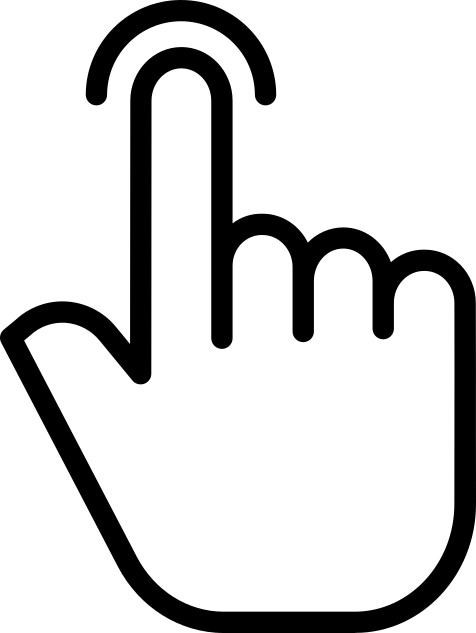
\includegraphics[width=0.10\textwidth]{static/dedo.png}} ;
    \node[const,below=of d] (nd) {\En{Hint}\Es{Pista}: $s \neq r$, $s \neq c$  } ;

    \node[latent, above=of d,yshift=-1.2cm, xshift=-1.3cm] (r) {
\includegraphics[width=0.12\textwidth]{static/regalo.png}} ;
    \node[const,above=of r] (nr) {\phantom{g}\En{Gift}\Es{Regalo}: $r$\phantom{g}} ;

    \node[latent, fill=black!30, above=of d,yshift=-1.2cm, xshift=1.3cm] (c) {
\includegraphics[width=0.12\textwidth]{static/cerradura.png}} ;
    \node[const,above=of c] (nc) {\phantom{g}\En{Election}\Es{Elección}: $c_1$\phantom{g}} ;

    \edge {r,c} {d};

         \node[factor, minimum size=0.8cm, xshift=-1.3cm, yshift=2.5cm] (p1) {
\includegraphics[width=0.075\textwidth]{static/cerradura.png}} ;
         \node[det, minimum size=0.8cm, yshift=2.5cm] (p2) {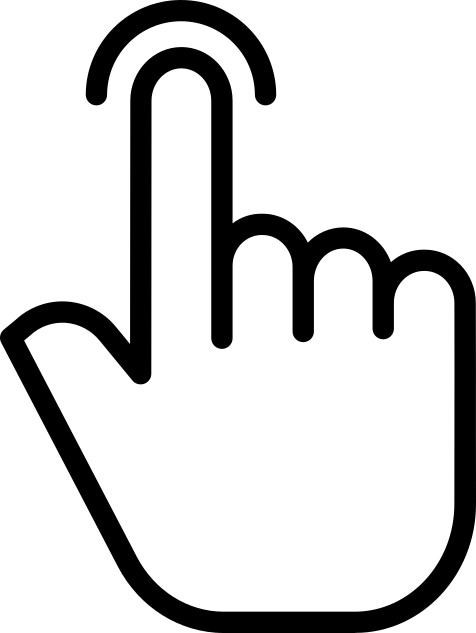
\includegraphics[width=0.085\textwidth]{static/dedo.png}} ;
         \node[factor, minimum size=0.8cm, xshift=1.3cm, yshift=2.5cm] (p3) {} ;
         \node[const, above=of p1, yshift=.05cm] (fp1) {$?$};
         \node[const, above=of p2, yshift=.05cm] (fp2) {$?$};
         \node[const, above=of p3, yshift=.05cm] (fp3) {$?$};
         \node[const, below=of p2, yshift=-.10cm, xshift=0.3cm] (dedo) {};

  }
  \caption{}
  \label{fig:modelo_causal}
  \end{subfigure}
 \begin{subfigure}[b]{0.32\textwidth}
\centering
\tikz{
\node[latent, draw=white, yshift=0.7cm] (b0) {$1$};
\node[latent,below=of b0,yshift=0.9cm, xshift=-1.5cm] (r1) {$r_1$};
{\color{black}\node[latent,draw=black,below=of b0,yshift=0.9cm] (r2) {$r_2$}; }
\node[latent,below=of b0,yshift=0.9cm, xshift=1.5cm] (r3) {$r_3$};
\node[latent, below=of r1, draw=white, yshift=0.7cm] (bc11) {$\frac{1}{3}$};
{\color{black}\node[latent, below=of r2, draw=white, yshift=0.7cm] (bc12) {$\frac{1}{3}$};}
\node[latent, below=of r3, draw=white, yshift=0.7cm] (bc13) {$\frac{1}{3}$};
\node[latent,below=of bc11,yshift=0.9cm, xshift=-0.5cm] (r1d2) {$s_2$};
{\color{black}\node[latent,draw=black,below=of bc11,yshift=0.9cm, xshift=0.5cm] (r1d3) {$s_3$};}
{\color{black}\node[latent, draw=black,below=of bc12,yshift=0.9cm] (r2d3) {$s_3$};}
\node[latent,below=of bc13,yshift=0.9cm] (r3d2) {$s_2$};

\node[latent,below=of r1d2,yshift=0.9cm,draw=white] (br1d2) {$\frac{1}{3}\frac{1}{2}$};
{\color{black}\node[latent,below=of r1d3,yshift=0.9cm, draw=white] (br1d3) {$\frac{1}{3}\frac{1}{2}$};}s
{\color{black}\node[latent,below=of r2d3,yshift=0.9cm,draw=white] (br2d3) {$\frac{1}{3}$};}
\node[latent,below=of r3d2,yshift=0.9cm,draw=white] (br3d2) {$\frac{1}{3}$};
\edge[-] {b0} {r1,r3};
\edge[-,draw=black] {b0} {r2};
\edge[-] {r1} {bc11};
\edge[-,draw=black] {r2} {bc12};
\edge[-] {r3} {bc13};
\edge[-] {bc11} {r1d2};
\edge[-,draw=black] {bc11} {r1d3};
\edge[-,draw=black] {bc12} {r2d3};
\edge[-] {bc13} {r3d2};
\edge[-] {r1d2} {br1d2};
\edge[-,draw=black] {r1d3} {br1d3};
\edge[-,draw=black] {r2d3} {br2d3};
\edge[-] {r3d2} {br3d2};
}
\caption{}
\label{fig:caminos_montyhall_compatibles}
\end{subfigure}
\
\begin{subfigure}[b]{0.34\textwidth}
\phantom{$P(s_j)$\hspace{0.7cm}g}$P(r_i, s_j)$\phantom{g}\hspace{0.9cm}$P(s_j)$
\centering
  \begin{tabular}{|c|c|c|c||c|} \hline  \setlength\tabcolsep{0.4cm}
 & \, $r_1$ \, &  \, $r_2$ \, & \, $r_3$ \, &  \\ \hline
  $\gray s_1$ & $\gray0$ & $\gray0$ & $\gray0$ &   $\gray 0$ \\ \hline
  $\bm{s_2}$ & $\bm{1/6}$ & $\bm{0}$ & $\bm{1/3}$ &  $\bm{1/2}$ \\  \hline
  $\gray s_3$ & $\gray1/6$ & $\gray1/3$ & $\gray0$ & $\gray1/2$ \\ \hline
  \end{tabular}

  \phantom{--}\\[0.1cm]

  \tikz{

         \node[factor, minimum size=0.8cm, xshift=-1.3cm] (p1) {
\includegraphics[width=0.075\textwidth]{static/cerradura.png}} ;
         \node[det, minimum size=0.8cm] (p2) {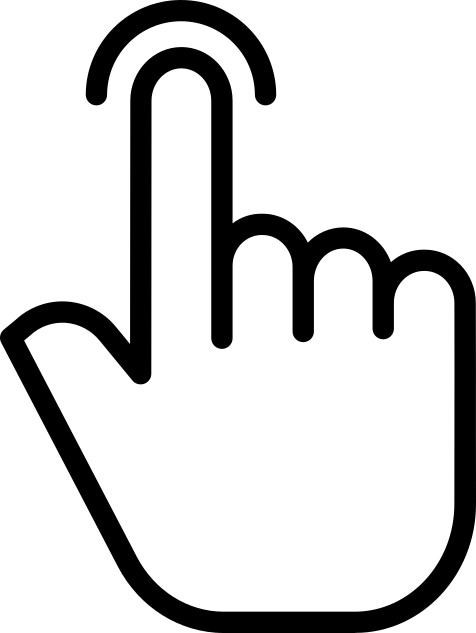
\includegraphics[width=0.085\textwidth]{static/dedo.png}} ;
         \node[factor, minimum size=0.8cm, xshift=1.3cm] (p3) {} ;
         \node[const, below=of p1, yshift=-.025cm] (fp1) {$1/3$};
         \node[const, below=of p2, yshift=-.025cm] (fp2) {$0$};
         \node[const, below=of p3, yshift=-.025cm] (fp3) {$2/3$};
         \node[const, above=of p2, yshift=.045cm] (title) {$P(r_i | s_2)=P(r_i,s_2)/P(s_2)$};

         \node[const, below=of p2, yshift=-.10cm, xshift=0.3cm] (dedo) {};

  }

\caption{}
\label{fig:f3}
\end{subfigure}
\caption{
Acuerdo intersubjetivo dada toda la información disponible (modelo causal y datos).
%
(\subref{fig:modelo_causal}) El modelo causal asegura que la pista $s$ no puede señalar la caja elegida $c$ (con la cerradura) ni la caja donde se encuentra el regalo $r$ (la hipótesis oculta): $s\neq c$ y $s\neq r$.
%
(\subref{fig:caminos_montyhall_compatibles}) Calculamos la creencia que maximiza la incertidumbre dado el modelo causal dividiendo la creencia en partes iguales en cada bifurcación de los universos paralelos.
%
(\subref{fig:f3}) La nueva creencia no es más que la creencia inicial (tabla) que sigue siendo compatible con el dato $s_2$ (renglón oscuro), expresada como 100\%
}
\label{fig:monty_hall}
\end{figure}

% Parrafo

A diferencia de los enfoques ad-hoc que seleccionan una única hipótesis (e.g.~por máxima verosimilitud), la aplicación estricta de las reglas de la probabilidad (enfoque bayesiano), considerando al mismo tiempo hipótesis mutuamente contradictorias (A y no A), permite que sea la sorpresa, única fuente de información, el filtro de las creencias previas.
%
En general, si tenemos $\text{Datos} = \{ \text{dato}_1, \text{dato}_2, \dots \}$,
%
\begin{equation} \label{eq:funcion_de_costo}
\underbrace{P(\text{\En{Hypothesis}\Es{Hipótesis}},\text{\En{Data}\Es{Datos}})}_{\hfrac{\text{\footnotesize\En{Initial belief compatible}\Es{Creencia compatible }}}{\text{\footnotesize \En{with the data}\Es{con los datos}}}} = \underbrace{P(\text{\En{Hypothesis}\Es{Hipótesis}})}_{\hfrac{\text{\footnotesize\En{Initial intersubjective}\Es{Acuerdo inter-}}}{\text{\footnotesize\En{agreement}\Es{subjetivo inicial}}}} \underbrace{P(\text{dato}_1 |\text{\En{Hypothesis}\Es{Hipótesis}})}_{\text{\footnotesize Predic\En{tion}\Es{ción} 1}} \, \underbrace{P(\text{dato}_2 | \text{dato}_1 , \text{\En{Hypothesis}\Es{Hipótesis}})}_{\text{\footnotesize Predic\En{tion}\Es{ción} 2}} \dots
\end{equation}

% Parrafo

\noindent
Si la predicción del dato observado es 1 (sorpresa nula), entonces preservamos toda nuestra creencia previa en esa hipótesis.
%
Si la predicción del dato observado es 0 (sorpresa total), entonces la hipótesis se hace falsa para siempre.
%
Le ocurre lo mismo que a las especies, de la extinción no se vuelve.


% Parrafo

Así como la evaluación de las hipótesis en probabilidad se hace a través de la secuencias de predicciones, la selección de las formas de vida en evolución también sigue un proceso de naturaleza multiplicativa, por secuencia de tasas de supervivencia y reproducción.
%
De hecho, el modelo estándar de evolución, conocido como \emph{replicator dynamic} \cite{taylor1978-replicatorDynamic}, es estructuralmente equivalente al teorema de Bayes, lo que llevó a autores reconocidos en ambas áreas a proponer el isomorfismo entre las teoría de la evolución y la inferencia bayesiana~\cite{czegel2019-bayesianEvolution, czegel2022-bayesDarwin}.
%
\begin{equation*} \footnotesize
\overbrace{P\Big(\hfrac{\text{Hipótesis o}}{\text{Forma de vida}}  \Big| \text{Datos}, \hfrac{\text{Modelo}}{\text{Causal}} \Big)}^{\hfrac{\text{\scriptsize Nueva proporción}}{\text{\scriptsize de la variante}}} = \frac{ \overbrace{P\Big(\text{Datos},  \Big|  \hfrac{\text{Hipótesis o}}{\text{Forma de vida}}  , \hfrac{\text{Modelo}}{\text{Causal}} \Big)}^{\hfrac{\text{\scriptsize Adaptabilidad de la}}{\text{\scriptsize variante a la realidad}}} \overbrace{P\Big(\hfrac{\text{Hipótesis o}}{\text{Forma de vida}} \Big|  \hfrac{\text{Modelo}}{\text{Causal}} \Big)}^{\hfrac{\text{\scriptsize Vieja proporción}}{\text{\scriptsize de la variante}}}}{\underbrace{P\Big(\text{Datos},  \hfrac{\text{\small Modelo}}{\text{\small Causal}} \Big)}_{\hfrac{\text{\scriptsize Proporción}}{\text{\scriptsize sobreviviente}}}}
\end{equation*}
%
Debido a que en los procesos multiplicativos los impactos de las pérdidas son más fuertes que los de las ganancias (por ejemplo, un único cero en la secuencia produce una extinción irreversible) veremos que existe una ventaja a favor de las variantes que reducen las fluctuaciones (sección ``\nameref{sec:propiedades_funcion_costo}''): por diversificación individual (\emph{propiedad epistémica}), por cooperación (\emph{propiedad evolutiva}), por especialización cooperativa (\emph{propiedad de especiación}), y por heterogeneidad cooperativa (\emph{propiedad ecológica}).
%
Durante mucho tiempo se creyó que la evolución de la cooperación estaba condicionada por un dilema.
%
En la siguiente sección veremos que no existe tal dilema debido a que en los procesos de selección multiplicativos, los individuos desertores aumentan las fluctuaciones de los cooperadores de quienes dependen, aumentando por lo tanto sus propias fluctuaciones y afectando negativamente su propia tasa de crecimiento de largo plazo (\emph{propiedad mayor}).

% Parrafo

\section{Propiedades de la función de costo epistémico-evolutiva} \label{sec:propiedades_funcion_costo}
Desde su origen, la vida adquirió una extraordinaria complejidad en términos de diversificación, cooperación, especialización y heterogeneidad.
%
Para ver por qué, veamos qué ocurre con un proceso multiplicativo.
%
Por ejemplo, supongamos que una casa de apuestas ofrece pagos $Q_c > 0$ y $Q_s > 0$ cuando una moneda sale Cara y Seca respectivamente y que los individuos se ven obligados a apostar en cada paso temporal todos sus recursos, asignando una proporción $b_c = b$ a Cara y $b_s = 1 - b$ a Seca (apostar solo un parte de los recursos puede mostrarse que tiene una solución equivalente).
%
Si nuestros recursos iniciales son $\omega_0$, los recursos que obtenemos con una apuestas $b \in [0,1]$ después de una Cara y una Seca es el producto de nuestros resultados.
%
 \begin{equation*}
\begin{split}
\omega_2(b) & = \underbrace{\omega_0 \, \overbrace{b \,  Q_c}^{\text{Cara}}}_{\omega_1(b)} \, \overbrace{(1-b) \, Q_s}^{\text{Seca}}
\end{split}
\end{equation*}
%
Las apuestas son entonces procesos multiplicativos.
%
Vamos a buscar las estrategias que maximizan la tasa de crecimiento de los recursos.

\subsection{Propiedad epistémica.}
Si comparamos los recursos de dos apuestas diferentes $b \neq d \in [0,1]$ luego de obtener $n_c$ Caras y $n_s$ Secas, en el tiempo $T = n_c + n_s$,
%
  \begin{equation}
\begin{split}
& \frac{\omega_T(b)}{\omega_T(d)} = \frac{\omega_0 \,  (b \,  \cancel{Q_c})^{n_c}  \,  ((1-b) \, \bcancel{Q_s})^{n_s}}{\omega_0 \,   (d \,  \cancel{Q_c})^{n_c}  \,  ((1-d) \, \bcancel{Q_s})^{n_s}}
\end{split}
\end{equation}
%
encontramos que el valor relativo de una apuesta respecto de la otra es independiente de los pagos $Q_c$ y $Q_s$ que ofrece la casa de apuestas!
%
Sí, lo que estamos diciendo es que podemos decidir la apuesta sin conocer los pagos.
%
En general, queremos la apuesta $b$ que maximiza la tasa de crecimiento $r(b)$,
%
\begin{figure}[ht!]
 \centering
 \begin{subfigure}[b]{0.50\textwidth}
  \begin{equation*}
\begin{split}
  \omega_0 \, r(b)^T &= \omega_0 \, (b \,  Q_c)^{n_c}  \,  ((1-b) \, Q_s)^{n_s}   \\
  r(b) &=(b \,  Q_c)^{n_c/T}  \,  ((1-b) \, Q_s)^{n_s/T}
\end{split}
\end{equation*}
 \end{subfigure}
 \begin{subfigure}[b]{0.49\textwidth}
  \begin{equation}
\begin{split}
\overbrace{\underset{b}{\text{arg max}} \phantom{T} r(b)}^{\hfrac{\text{\scriptsize \En{Optimal}\Es{Apuesta}}}{\text{\scriptsize \En{bet}\Es{óptima}}}} \ = \overbrace{n_c/T}^{\hfrac{\text{\scriptsize \En{Observed}\Es{Frecuencia}}}{\text{\scriptsize \En{frequency}\Es{observada}}}}
\end{split}
\end{equation}
 \end{subfigure}
\end{figure}

% Parrafo

\noindent
En efecto, no importa los pagos que ofrezca la casa de apuestas, la apuesta óptima  $b^{*}$ es la que divide los recursos en la misma proporción que la frecuencia observada, $b^{*} = n_c/T$, la que en el largo plazo tiende a la frecuencia típica $\lim_{T \rightarrow \infty} n_c/T = p$.
%
Ésta es la \emph{propiedad epistémica} que le permite a la teoría de la probabilidad adquirir conocimiento sobre el mundo, pues al evaluar las hipótesis individuales en base al producto de las sorpresas se produce una ventaja a favor de las hipótesis que diversifican la predicción en la misma proporción que la frecuencia observada.
%
Del mismo modo, el proceso de selección evolutiva por secuencias de tasas de crecimiento y reproducción, produce la emergencia de formas de vida que reducen las fluctuaciones a través de la diversificación individual.

% Parrafo

Por ejemplo, supongamos que la casa de apuestas ofrece $Q_c = 3$ por Caras y $Q_s = 1.2$ por Secas.
%
Si sabemos que la moneda es no sesgada, lo mejor que podemos hacer a largo plazo es dividir los recursos en partes iguales, $b = p = 0.5$.
% bien con estos parámetros el valor esperado es positivo, $( Q_c \, b \, p + Q_s \, (1-b) \, (1-p)) = 1.05$,
En este caso, sin embargo, no podemos ganar este juego individualmente debido a que las ganancias de 50\% con Caras ($1.5 = Q_c \, b$) no alcanza para compensar las caídas de 40\% que sufrimos con Secas ($0.6 = Q_s \, (1-b)$).
%
Incluso con el comportamiento óptimo, individualmente las trayectorias de los recursos caen a una tasa cercana a $5\%$, pues $r(b) \approx 0.95$ (figura~\ref{fig:coop}).

% Parrafo

\subsection{Propiedad evolutiva.}
A pesar de que la diversificación individual no es suficiente para ganar este juego, la vida encontró estrategias para florecer en casos como estos, reduciendo aun más las fluctuaciones individuales mediante cooperación~\cite{yaari2010-cooperationEvolution, peters-cooperation2019.03.04}.
%
Por ejemplo, si los individuos de un grupo de tamaño $N$ redistribuyen los recursos en partes iguales luego de apostar, la riqueza de cada uno pasa a ser el promedio de todos los recursos luego de que $m_c$ y $m_s$ individuos obtienen Cara y Seca respectivamente, con $m_c + m_s = N$.
%
\begin{equation}
\begin{split}
\omega_{T+1}(N,b) & = \frac{1}{N} \overbrace{\bigg( m_c \, \omega_{T}(N,b) \, Q_c  \, b + m_s \, \omega_{T}(N,b) \, Q_s  \, (1-b)  \bigg)}^{\hfrac{\text{\footnotesize \phantom{g}\En{Sum of all resources}\Es{Suma de todos los recursos}\phantom{g} }}{\text{\scriptsize (\En{with}\Es{con} $m_s$ \En{Heads}\Es{Caras} y $m_s$ \En{Tails}\Es{Secas})}}} \\
& =\omega_T(N,b) \, \underbrace{\left( \frac{m_c}{N}   Q_c  \, b + \frac{m_s}{N} \, Q_s  \, (1-b)  \right)}_{\text{\scriptsize\phantom{Tg} $r(N,b)$: \En{growth rate}\Es{Tasa de crecimiento}  \phantom{Tg}}} \\[0.3cm]
\end{split}
\end{equation}
%
Y la tasa de crecimiento de los individuos pasa a ser el promedio de todos los resultados del grupo.
%
La reducción de fluctuaciones que genera este simple acto de intercambio de recursos, hace que la tasa de crecimiento de todos los individuos se vuelve positiva.
%
Ésta es la \emph{propiedad evolutiva}.
%
A través de la cooperación podemos reducir aun más las fluctuaciones, aumentando así la tasa de crecimiento de todos sus miembros.
%
\begin{figure}[ht!]
\vspace{-0.1cm}
\centering
 \begin{subfigure}[c]{0.50\textwidth}
 \centering
  \begin{tabular}{|l|c|c|c|c|c|}
     \hline
         & {\small $\omega_0$} & {\small \  $\Delta$}  & {\small \, $\omega_1(b)$ } & {\small \  $\Delta$}  & {\small \,  $\omega_2(b)$ }  \\ \hline \hline
        A no-coop& $1$ & $1.5$ &  $1.5$ & $0.6$ & $\bm{0.9}$ \\ \hline
        B no-coop & $1$ & $0.6$ & $0.6$ & $1.5$ & $\bm{0.9}$ \\ \hline\hline
        A coop & $1$ & $1.5$ & $1.05$ & $0.6$ & $\bm{1.1}$ \\ \hline
        B coop & $1$ & $0.6$ & $1.05$ & $1.5$ & $\bm{1.1}$\\ \hline
\end{tabular}
 \end{subfigure}
 \begin{subfigure}[c]{0.45\textwidth}
\begin{flushright}
 \includegraphics[width=0.9\linewidth]{figures/pdf/ergodicity_individual_trayectories.pdf}
 \end{flushright}
 \end{subfigure}
 \caption{
 La cooperación le permite a los individuos alcanzar tasas de crecimiento que jamás obtendrían solos.
 %
 En la tabla (izquierda) $\Delta$ representa el cambio en los recursos que sufren los individuos de forma aleatoria, con $b=p=0.5$.
 %
 En la figura (derecha), las curvas de colores son las trayectoria de los recursos jugando individualmente, y la recta negra es la trayectoria de los recursos individuales jugando en grupos cooperativos grandes.
 }
 \label{fig:coop}
 \vspace{-0.1cm}
 \end{figure}

% Parrafo

\subsection{Propiedad de especiación.}
Si bien jugando individualmente nos veíamos obligados a apostar ignorando los pagos que ofrece la casa de apuestas, una vez que emerge la cooperación deja de ser necesario reducir las fluctuaciones por diversificación individual y aparece una ventaja a favor de la especialización cooperativa, que permite sacar provecho de la mejor opción disponible, aumentando aún más la tasa de crecimiento de todos los individuos del grupo cooperativo.
%
\begin{figure}[ht!]
\centering
  \begin{subfigure}[c]{0.45\textwidth}
\begin{flushright}
 \includegraphics[width=1\linewidth]{figures/tasa-temporal2.pdf}
 \end{flushright}
 \end{subfigure}
 \caption{
Tasa de crecimiento para grupos de tamaño 1 a 5 (colores), para todas las posibles apuestas (eje x). A medida que aumenta el tamaño del grupo, la apuesta óptima se va especializando hacia la opción mejor paga por la casa de apuesta.
 }
 \label{fig:esp}
 \vspace{-0.1cm}
 \end{figure}
%
A medida que el tamaño del grupo cooperativo crece, la apuesta óptima se va especializando hacia la mejor opción disponible (figura~\ref{fig:esp}).
%
Ésta es la \emph{propiedad de especiación}.
%
Cuando el tamaño del grupo tiende a infinito, la tasa de crecimiento pasa a ser la media aritmética de los posibles resultados de las apuestas.
%
\begin{equation}
\lim_{N \rightarrow \infty} r(N,b) = p \,  Q_c  \, b + (1-p) \, Q_s  \, (1-b)
\end{equation}
%
Y la puesta óptima es apostar todo a la mejor opción, $b^* =1$.

% Parrafo

\subsection{Propiedad ecológica.}
En este caso, todos los individuos están sujetos a procesos estocásticos que, si bien son independientes, tiene para todos ellos la misma probabilidad que no cambia en el tiempo.
%
En la naturaleza, por el contrario, estamos expuestos a variabilidades espacio-temporales, como las estaciones del año.
%
Para dar un ejemplo, supongamos que la moneda oscila entre dos probabilidades de que salga Cara, $p_1 = 0.2$ y $p_2 = 0.6$.
%
En los pasos temporales impares, la moneda tiene probabilidad $p_1$ en el hemisferio A y $p_2$ en el hemisferio B.
%
Y a la inversa en los pasos temporales pares.
%
En casos como estos la variabilidad del proceso produce una ventaja adicional en favor de los grupos con mayor heterogeneidad interna.
%
Ésta es la \emph{propiedad ecológica}.
%
Sea $h$ la proporción de individuos en el hemisferio A.
%
La tasa de crecimiento en un ejemplo simple, en el que el tamaño del grupo es infinito y en el que los individuos se especializan la apuesta correspondiente a la etapa del ciclo que experimentan, es
%
\begin{figure}[ht!]
\vspace{0cm}
\centering
 \begin{subfigure}[c]{0.44\textwidth}
 \begin{align*}
 r_{1}(h) = & \  \overbrace{(\underbrace{h \, (1-p_1) \, Q_s}_{\hfrac{\text{En hemisferio A se}}{\text{especializan en Secas}}} + \underbrace{(1-h) \, p_2 \, Q_c )}_{\hfrac{\text{En el hemisferio B se}}{\text{especializan en Caras}}} }^{\text{Tasa de crecimiento en tiempos 1}} \\
 r_{2}(h) = & \ \overbrace{ (\underbrace{h \ p_2 \ Q_c}_{\hfrac{\text{En  hemisferio A se}}{\text{especializan en Caras}}} + \, \underbrace{(1-h) \, (1-p_1) \, Q_s}_{\hfrac{\text{En  hemisferio B se}}{\text{especializan en Secas}}} )}^{\text{Tasa de crecimiento en tiempos 2}} \\
 r(h) = & \ \overbrace{r_{1}(h)^{1/2} \ r_2(h)^{1/2}}^{\text{Tasa de crecimiento}}
\end{align*}
 \end{subfigure}
 \hspace{0.2cm}
  \begin{subfigure}[c]{0.44\textwidth}
\begin{flushright}
 \includegraphics[width=1\linewidth]{figures/pdf/diversificacionCooperativa.pdf}
 \end{flushright}
 \end{subfigure}
 \caption{
 En la figura vemos la tasa de crecimiento de los individuos en función de la proporción de individuos en el hemisferio A. La tasa de crecimiento se maximiza cuando la heterogeneidad entre individuos es máxima.
 }
 \label{fig:divCoop}
 \vspace{-0.1cm}
 \end{figure}


Esta tasa de crecimiento se maximiza cuando la distribución entre hemisferios es en partes iguales, con $h=0.5$ (figura~\ref{fig:divCoop}).
%

\subsection{Propiedad mayor y menor.}
Durante mucho tiempo se creyó que para que la cooperación evolucione debía resolverse primero lo que se conoce como ``dilema del prisionero''.
%
En él, cooperar implica un costo $c$ para que el otro individuo reciba un beneficio de valor $v$, con $v > c$, y desertar significa negarse a cooperar y no conlleva ningún costo (ver matriz en figura~\ref{fig:desert}).
%
 \begin{equation*}
  \bordermatrix{ _{\text{\tiny Focal}}{\rotatebox{45}{\text{$\mid$}}}^{\text{\tiny \En{Other}\Es{Otro}}} \hspace{-0.5cm} & C & D \cr
      \ \ \   C & v-c & -c \cr
      \ \ \ D & v & 0 }
\end{equation*}
%
Este ejemplo es una dilema debido a que individualmente desertar siempre es mejor que cooperar, a pesar de que la mutua cooperación sea mejor que la mutua deserción.

% Parrafo

En nuestro ejemplo de las apuestas, habría una tentación por desertar: dejar de aportar al fondo común mientras se sigue recibiendo la cuota del fondo común.
%
Si la evolución estuviera sujeta a un dilema del prisionero, entonces desertar en grupos enteramente cooperativos debería ofrecer al individuo una tasa de crecimiento más alta que cooperar.
%
En la figura~\ref{fig:desert} mostramos la tasa de crecimiento de individuos en grupos cooperativos de tamaño 100 con 0, 1 y 2 desertores.
%
\begin{figure}[ht!]
\centering
 \begin{subfigure}[c]{0.45\textwidth} \centering
  \includegraphics[width=\linewidth]{figures/pdf/ergodicity_desertion.pdf}
  \end{subfigure}
 \caption{
Tasa de crecimiento de los individuos dentro de grupos cooperativos (colores) con 0, 1 y 2 desertores. Las curvas con mayor variabilidad son los individuos desertores, el resto son los cooperadores.}
 \label{fig:desert}
 \end{figure}
 %
Allí se puede observar que los desertores tienen una tasa de crecimiento menor que la tenían cuando cooperaban (\emph{propiedad mayor}), a pesar de que inicialmente obtienen un beneficio circunstancial (\emph{propiedad menor}).
%
El primer agente que decide desertar unilateralmente (grupo azul con 1 desertor) reduce su tasa de crecimiento y sus recursos están por debajo de los recursos que tenía previamente dentro del grupo enteramente cooperador (grupo verde con 0 desertores).
%
La reducción de recursos le ocurre incluso al segundo individuo que cambia de comportamiento cooperador a desertor.
%
Es decir, los bienes comunes no tiene la estructura del dilema del prisionero como habitualmente se afirma en la literatura.
%
Bajo procesos de selección multiplicativa no se puede sacar provecho mediante la deserción porque, al aumentar las fluctuaciones los cooperadores de quienes se depende, aumenta también las propias fluctuaciones afectando negativamente la propia tasa de crecimiento de largo plazo.
%
En todos los casos, la tasa de crecimiento se maximiza mediante mutua cooperación.


\section{Consecuencias de las propiedades epistémico-evolutivas}

Las propiedades de la función de costo epistémico-evolutiva no son solo teóricas, tiene consecuencia concretas para la vida y el conocimiento.

\subsection{Transiciones evolutivas mayores}

En el último tercio de la historia del Universo, hace aproximadamente 4000 millones de años, apareció en la tierra una organización de la materia capaz de auto-replicarse.
%
El crecimiento de estos linajes siguieron procesos multiplicativos y ruidosos: secuencias de tasas de supervivencia y reproducción.
%
Las mutaciones producidas durante la replicación diversificaron las formas de vida, y las tasas de crecimiento de las diferentes estrategias favorecieron a aquellas mejor adaptadas al ambiente.
%
Desde aquel momento hasta ahora la vida adquirió una extraordinaria complejidad.

%

\begin{figure}[ht!]
    \centering
    \begin{subfigure}[b]{0.65\textwidth}
    \includegraphics[width=\linewidth]{static/biomassBarOn.png}
    \end{subfigure}
    \caption{
	Distribución de la biomasa en la Tierra estimada por Bar-On et al.~\cite{barOn2018-biomass}.
    }
    \label{fig:biomass}
\end{figure}

% Parrafo

La complejidad actual de la vida es consecuencia de una serie de \emph{transiciones evolutivas mayores} en las que entidades capaces de autorreplicación luego de la transición pasan a formar parte de unidades cooperativas indisolubles~\cite{maynardSmith1995-majorTransitions, szathmary1995-evolutionaryTransitions, szathmary2015-evolutionaryTransitions} (figura \ref{fig:trans}).
%
De hecho, nuestra propia vida depende de varios niveles de cooperación con especialización heterogénea, sin los cuales no somos capaces de sobrevivir: la unión de nuestras células con las mitocondrias y la emergencia de la diferenciación celular; nuestro organismo multicelular y la emergencia de los órganos; nuestra sociedad y la emergencia de los roles y grupos; la coexistencia entre especies y la emergencia de los ecosistemas.
%
%La simbiosis entre entre plantas y hongos micorrízicos arbusculares (AM) es el mutualismo (cooperación entre especies) más extendida del mundo.
% %
% La gran mayoría de las plantas terrestres forman estas interacciones.
% %
% Las plantas suministran carbohidratos esenciales para la supervivencia y el crecimiento de los hongos AM \cite{parniske2008-arbuscularMycorrhiza}.
% %
% Y los hongos AM proporcionan a sus plantas hospedadoras nutrientes minerales, como fósforo o nitrógeno, y otros beneficios como protección contra el estrés biótico (patógenos y herbívoros) y abiótico (por ejemplo, sequía)~\cite{smith2010-arbuscularMycorrhizas}.
% %
% % Parrafo
% Esta asociación evolucionó mucho antes que los mutualismos animales, y habría sido una pieza clave para el poblamiento de las plantas en la tierra.
% %
% A diferencia de las economías humanas, que dependen de la cognición para tomar decisiones, los comerciantes de este mercado subterráneo regatean, piden prestado y hacen trampas, todo ello sin pensar.
% %
% En esta relación, ambas partes interactúan con múltiples socios y la cooperación se estabiliza en ambas direcciones a través de recompensas mutuas por servicios de mayor calidad~\cite{kiers2011-reciprocalRewards}.
%
\begin{figure}[ht!]
\centering
    \centering
  \scalebox{1}{
  \tikz{
      \node[accion] (i1) {} ;
      \node[accion, yshift=0.6cm, xshift=0.4cm] (i2) {} ;
      \node[accion, yshift=0.6cm, xshift=-0.4cm] (i3) {} ;
      \node[const, yshift=0.3cm, xshift=0.4cm] (i) {};

      \node[const, yshift=-0.65cm] (ni) {$\hfrac{\text{Individuos}}{\text{solitarios}}$};

      \node[const, yshift=0.65cm, xshift=1.5cm] (m1) {$\hfrac{\text{Formación}}{\text{de grupos}}$};

      \node[const, right=of i, xshift=2cm] (c) {};
      \node[accion, below=of c, yshift=0.35cm, xshift=0.4cm] (c1) {} ;
      \node[accion, above=of c, yshift=-0.35cm, xshift=0.6cm] (c2) {} ;
      \node[accion, above=of c, yshift=-0.35cm, xshift=0.2cm] (c3) {} ;
      \node[const, right=of c, xshift=0.6cm] (cc) {};

      \node[const, right=of ni, xshift=1.3cm] (nc) {$\hfrac{\text{Grupos}}{\text{cooperativos}}$};

      \node[const, right=of m1, xshift=1.2cm] (m2) {$\hfrac{\text{Transición}}{\text{mayor}}$};

      \node[const, right=of cc, xshift=2cm] (t) {};
      \node[accion, below=of t, yshift=0.35cm, xshift=0.4cm] (t1) {} ;
      \node[accion, above=of t, yshift=-0.35cm, xshift=0.6cm] (t2) {} ;
      \node[accion, above=of t, yshift=-0.35cm, xshift=0.2cm] (t3) {} ;

      \node[const, right=of nc, xshift=1.1cm] (nt) {$\hfrac{\text{Unidad de}}{\text{nivel superior}}$};

      \edge {i} {c};
      \edge {cc} {t};

      \plate {transition} {(t1)(t2)(t3)} {}; %
      }
  }

  \vspace{0.2cm}

 \begin{subfigure}[b]{0.25\textwidth} \centering
  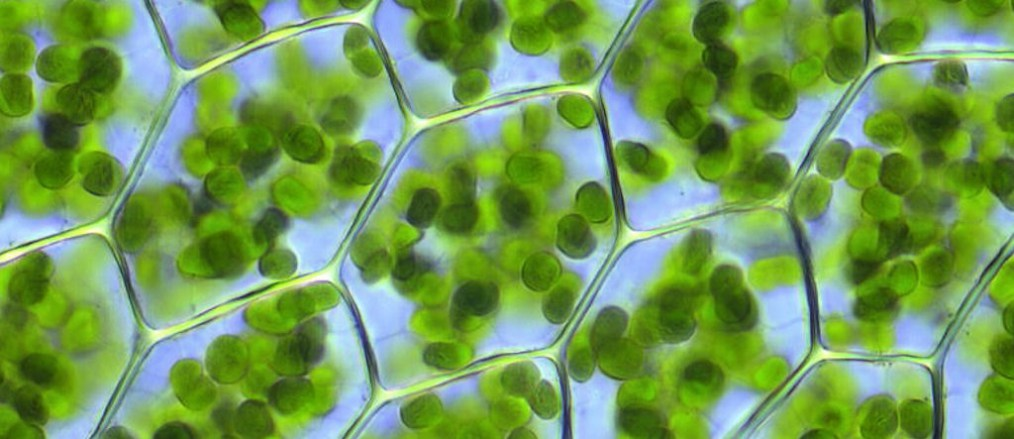
\includegraphics[width=\linewidth]{static/cloroplastos.jpg}
  \caption*{\En{Eukaryotic cells}\Es{Células eucariota}}
  \end{subfigure}
 \begin{subfigure}[b]{0.23\textwidth} \centering
  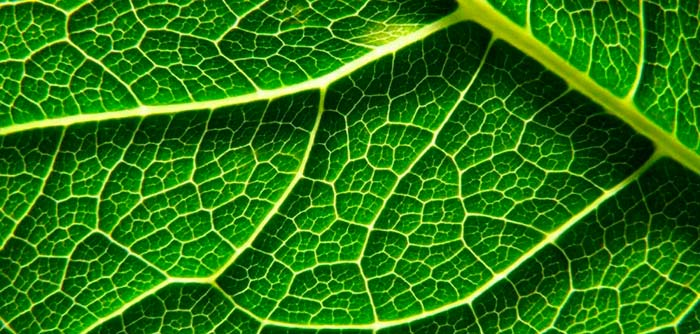
\includegraphics[width=\linewidth]{static/fotosintesis.jpg}
  \caption*{\En{Organisms}\Es{Organismos}}
  \end{subfigure}
  \begin{subfigure}[b]{0.235\textwidth} \centering
 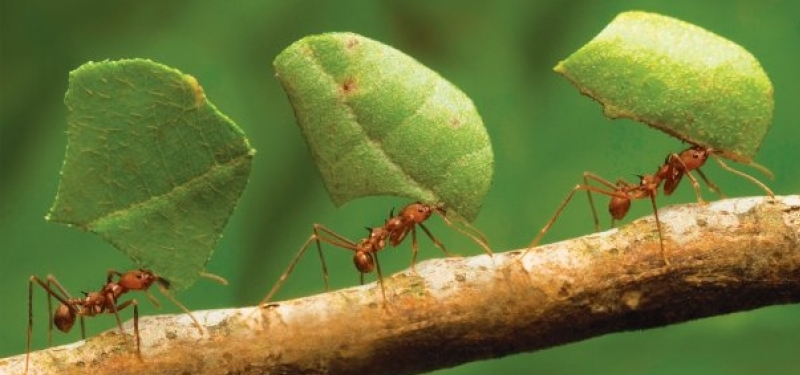
\includegraphics[width=\linewidth]{static/hormigas2.jpg}
  \caption*{\En{Societies}\Es{Sociedades}}
 \end{subfigure}
 \begin{subfigure}[b]{0.235\textwidth} \centering
 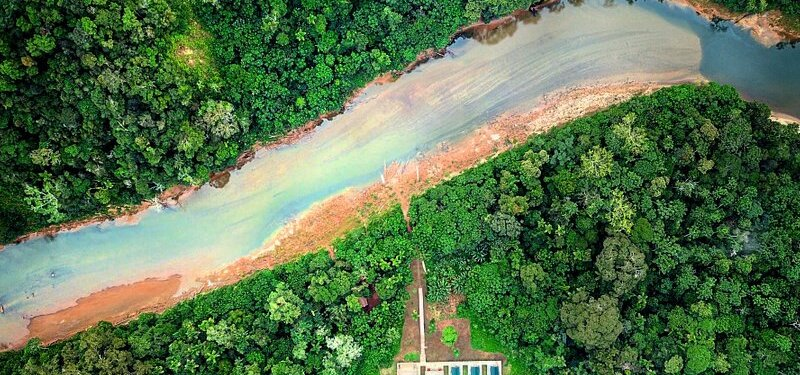
\includegraphics[width=\linewidth]{static/tsimane2.jpg}
  \caption*{\En{Ecosystems}\Es{Ecosistemas}}
 \end{subfigure}
 \caption{
Esquema de las transiciones evolutivas mayores (arriba) y ejemplos de transiciones evolutivas mayores (abajo).
 }
 \label{fig:trans}
 \vspace{-0.3cm}
 \end{figure}
¿Cómo se explica esta tendencia de la vida a favor de la diversificación y la especialización heterogénea cooperativa?

% Parrafo

La \emph{propiedad mayor} nos ofrece un argumento para explicar la emergencia permanente de las \emph{transiciones evolutivas mayores} a lo largo de la historia de la vida.
%
En la sección anterior hemos visto que en los procesos de selección epistémico-evolutivos existe una ventaja a favor de las variantes que reducen las fluctuaciones por diversificación o por especialización heterogénea cooperativa.
%
Si bien ciertas coyunturas pueden favorecer a la deserción en el corto plazo (\emph{propiedad menor}), a largo plazo afectan negativamente su propia tasa de crecimiento debido a que su propio comportamiento aumenta las fluctuaciones de los cooperadores de quienes dependen, aumentando al así sus propias fluctuaciones (\emph{propiedad mayor}).

% Parrafo

% Pero también permite explicar la emergencia de \emph{transiciones epistémicas mayores} en la historia del conocimiento, en las que hipótesis individuales se agregan para formar hipótesis de nivel superior a través del intercambio de conocimientos.
% %
% Por otro lado, la propiedad menor nos ofrece un argumento para explicar la ventaja circunstancial que las variantes desertoras pueden obtener individualmente en el corto plazo y las crisis que su emergencia produce a nivel global en el largo plazo.
%
%
% De forma similar, la propiedad mayor nos ofrece un argumento para explicar la emergencia permanente de las \emph{transiciones epistémicas mayores} en la historia del conocimiento.
%

De forma similar, la evaluación de hipótesis en la teoría de la probabilidad también produce la emergencia de unidades cooperativas de nivel superior: las hipótesis individuales forman variables, las variables forman modelos causales y los sistemas de modelos causales forman teorías.
%
Esto ocurre gracias a que las hipótesis de nivel superior reducen las fluctuaciones realizando las predicciones con el aporte de todas las hipótesis de nivel inferior que la componen.
%
Por la regla de la suma, la predicción que hace un modelo del próximo dato es
%
\begin{equation*}
\begin{split}
P(d_{n+1}|d_1 \dots d_n, \text{Model\Es{o}}) = \sum^{\text{\En{Hypothesis}\Es{Hipótesis}}}_h P(d_{n+1}| d_1 \dots d_n, h, \text{Model\Es{o}}) P(h|d_1 \dots d_n, \text{Model\Es{o}})
%\\ P(d_{n+1}|d_1 \dots d_n, \text{\En{Theory}\Es{Teoría}}) = \sum^{\text{\En{Models}\Es{Modelos}}}_m P(d_{n+1}| h, d_1 \dots d_n, \text{Model\Es{o}}) P(h|d_1 \dots d_n, \text{Model\Es{o}})
\end{split}
\end{equation*}
%
Al realizar la predicción con la contribución de todas las hipótesis de nivel inferior, los modelos reducen las posibilidades de introducir valores extremos (un cero) en los procesos de selección multiplicativo a los que están sujetos (ecuación \ref{eq:funcion_de_costo}), produciendo mejores resultados que los que se obtendrían con una de ellas individualmente.

% Parrafo

La emergencia de la cultural en evolución puede ser vista como una \emph{transición epistémica mayor}.
%
En la historia del ser humano la cooperación epistémica, por transmisión de conocimiento entre individuos, tuvo un efecto positivo radical para nuestra especie: antes estuvimos en grave peligro de extinción, luego fuimos capaces de ocupar todos los nichos ecológicos de la tierra.
%
Veremos que los eventos históricos en los que se produjeron pérdidas masivas de diversidad cultural estuvieron seguidos por graves crisis socio-ecológicas.
%
Actualmente, a pesar de todos los avances, la ciencia metropolitana sigue siendo incapaz de compensar la masiva pérdida de los conocimientos milenarios producida durante la colonial-modernidad, y la crisis ecológica actual no deja de profundizarse.
%
En definitiva, la ventaja a favor de la diversidad y la cooperación no es solo teórica, es fundamentalmente práctica.


\subsection{Coevolución genético-cultual y transición epistémica mayor}

Antes de la transición cultural, estábamos en grave peligro de extinción, lo que se evidencia en la baja diversidad del genoma humano, respecto incluso de los homininos más cercanos~\cite{hrdy2009-mothers}.
%
Pero cuando el conocimiento, que antes debía ser redescubierto individualmente, pasó a ser un recurso común transmitido de generación en generación, comenzamos a ser capaces de ocupar todos los nichos ecológicos de la tierra como ningún otro vertebrado terrestre lo había logrado antes.
%
Organizados en pequeñas sociedades nómadas, logramos llegar caminando de África hasta sud América (flechas de la figura~\ref{fig:poblamiento}).

% % Parrafo
%
% \begin{figure}[ht!]
%     \centering
%     \begin{subfigure}[b]{0.6\textwidth}
%      \includegraphics[width=\textwidth]{figures/agricultura.pdf}
%      \label{fig:agricultura}
%     \end{subfigure}
% %     \begin{subfigure}[b]{0.40\textwidth}
% %     \includegraphics[width=\textwidth]{static/polynesia.png}
% %     \caption{Poblamiento del oc\'eano Pac\'ifico}
% %     \label{fig:polynesia}
% %     \end{subfigure}
%     \caption{
%     Poblamiento humano (flechas) y surgimientos independientes de la agricultura (puntos).
%     Proyecci\'on poli\'edrica de la tierra que conserva los tama\~nos relativos de los continentes.
%     %Las felchas indican el poblamiento, desde África a Asia, y de Asia hacia Ocean\'ia y Am\'erica.
%     %Los puntos rojos indican surgimiento independiente de agricultura.
%     %El mapa de la figura~\ref{fig:polynesia}, desarrollado por Thorsby~\cite{thorsby2016-polynesiaAmerica}, muestra el poblamiento de la Polynesia y los contactos con Ámerica evidenciados en el material gen\'eticos.
%     }%
%     \label{fig:poblamiento}
% \end{figure}
%

% Parrafo

La cultura es información no-genética que se transmite por vía social, de un individuo a otro.
%
Estos sistemas de procesamiento de información distribuida no son exclusivos de los seres humanos.
% %
Muchos animales son capaces de transmitir información por vía social, lo que produce la emergencia de tradiciones simples.
% %
En algunas como las ballenas, delfines, primates y aves, las tradiciones pueden ser bastante complejas, llegando a desarrollar un conjunto amplio de conocimientos que se adquieren primero por experiencia individual y luego son imitados por el resto~\cite{aplin2022-birdsCulture}.
%
Todas ellas, sin embargo, son manifiestamente más simples que la cultura humana.

% Parrafo

A diferencia de otros animales, los humanos acumulamos adaptaciones culturales, modificaciones sucesivas persistentes en el tiempo, produciendo sistemas culturales cada vez más complejos.
%
Ciertamente existen muchas adaptaciones raras, que son particulares a ciertas especies.
%
Pero los elementos que son realmente buenos, como el ojo, han evolucionado repetidamente entre las millones de especies animales del mundo.
%
Entonces, dado que la cultura ha hecho a los humanos extraordinariamente exitosos, ¿Por qué las otras especies no han adquirido esas capacidades?
%
¿Por qué solo los humanos?

% Parrafo: Co-evolución.

Entre los hominoides, los humanos se distinguen por una serie de rasgos que incluyen prolongados períodos juveniles, intervalos cortos entre nacimientos y una prolongada vida posreproductiva~\cite{Jones2011}.
%
Para explicar la integraci\'on de los procesos biol\'ogicos, cognitivos y sociales que permite a los humanos desarrollar culturas complejas ha sido necesario un proceso extenso de \emph{coevoluci\'on gen\'etico-cultural}.
%
%Es un error creer que primero evolucionó la naturaleza humana y luego desarrollamos la cultura.
%
La evolución del lenguaje es un ejemplo claro.
%
Las características genética que nos permiten escuchar, hablar y aprender el lenguaje serían inútiles sin lenguajes complejos para aprender.
%
Y a la inversa, para que evolucionen estas características innatas es necesario la presencia previa de alguna lengua primitiva que proporcionara una entorno cultural que presionara a favor de la selección de mejores habilidades lingüísticas innatas.
%
A través de rondas repetidas de coevolución, surgieron lenguajes complejos y el costoso aparato necesario para operarlos.

% Parrafo: Origen de las caracterisitcas

Antes del surgimiento de los humanos anat\'omicamente modernos (masa cerebral actual) y de los humanos conductualmente modernos (lenguaje), surgi\'o en África una linaje emocionalmente moderno, con capacidades para el entendimiento mutuo~\cite{hrdy2020-emotionallyModern}.
%
A diferencia de nuestros parientes m\'as cercanos (chimpanc\'es, bonobos, gorilas y orangutanes), en los que la crianza está bajo supervisión estricta de la madre, hace aproximadamente 3.5 millones de años, nuestros ancestros comenzaron a desarrollar un tipo de crianza cooperativa.
%
Esta forma de crianza cooperativa produjo un ambiente que favoreci\'o la selecci\'on de j\'ovenes capaces de monitorear y comprender las intenciones de los dem\'as, y de trasmitir a sus cuidadadores sus propias necesidades, dando inicio a un largo proceso de coevoluci\'on gen\'etico-cultural~\cite{hrdy2020-emotionallyModern}.
%
Hoy la capacidades para desarrollar culturas complejas son parte de nuestra biología.

% Parrafo

La comprensi\'on mutua, la imitaci\'on y el lenguaje permitieron la transmisi\'on de conocimientos basados en la experiencia de otros (\emph{aprendizaje social}), dando inicio a un proceso inter-generacional de acumulación de innovaciones que permiti\'o a las poblaciones humanas adaptarse r\'apidamente a los cambiantes contextos ambientales.
%
Lo que antes debía ser redescubierto una y otra vez mediante costosa experiencia individual, ahora podía ser transmitido a la siguiente generación.
%
%$La capacidad de adquirir comportamientos basados en la experiencia de otros sin tener que re-construirlos cada vez por prueba y error conduce un proceso de evolución y acumulativa cultural que permite a las poblaciones humanas adaptarse rápidamente ante cambios bruscos en el ambiente o migraciones a nuevos entornos.
% Parrafo
En las culturas humanas, la acumulación de innovaciones produce un repertorio tecnológico que nadie es capaz de redescubrir individualmente en un período de vida, incluso en las sociedades cazadoras recolectoras aparentemente simples.

% Parrafo

En la breve historia del ser humano, la experiencia acumulada por comunidades alrededor del mundo condujo, de forma independiente, a una obligación universal de dar y de recibir~\cite{mauss1923-leDon}.
%
La ``obligación de reciprocidad'' se refiere a un fenómeno antropológico observado en todas las culturas alrededor del mundo mediante el cual las personas produce una necesidad de devolver favores, servicios o regalos recibidos.
%
Esta práctica es esencial para el sostenimiento de todos los sistemas económicos, desde las sociedades cazadoras recolectoras hasta las sociedades capitalistas.

% Parrafo

La teor\'ia de la probabilidad nace en 1648 justamente de un debate respecto del \emph{precio justo} en contextos de incertidumbre.
%
Pascal y Fermat concluyeron que para que el intercambio sea justo el valor de los favores debe ser inversamente proporcional a la probabilidad de hacer el favor.
%
Ofrecer pagos inversos a la probabilidad ($Q_x = p_x^{-1}$) tiene la propiedad de garantizar la coexistencia entre una casa de apuestas y un conjunto infinito de individuos cooperativos.
%
Sin importar la apuesta $b$ que se elija, la tasa de crecimiento de un grupo cooperativo de tamaño infinito es siempre 1.
%
En caso de que existan dos opciones $A$ y $B$, la tasa de crecimiento cooperativa es
\begin{equation}
\cancel{p_{\text{A}}} \,  \cancel{Q^*_{\text{A}}} \, b + \bcancel{p_{\text{B}}} \, \bcancel{Q^*_{\text{B}}}  \, (1-b) = b + (1-b)  = 1
\end{equation}

% Parrafo

Las tecnolog\'ias de reciprocidad ecol\'ogica produjeron la aparici\'on independiente de la domesticaci\'on de especies animales y vegetales, el desarrollo de caracteres gen\'eticos que surgen como resultado de una interacci\'on simbi\'otica prolongada entre las especies.
%
Así es cómo la agricultura surgi\'o de forma paralela e independiente en los seis grandes sistemas geogr\'aficos de la tierra: en África subsahariana, Oriente medio, China, Oceanía, América del Norte y América del Sur (puntos rojos de la figura~\ref{fig:poblamiento}).
%
All\'i se desarrollaron los principales centros poblacionales de la humanidad.
% %
El aumento de la poblaci\'on intensificó aun más los procesos de evolución cultural acumulativa, haciendo de estas regiones los principales centros tecnológicos de la humanidad.

% Parrafo

Los estudios comparados muestran que las instituciones capaces de administrar exitosamente los bienes comunes y establecer relaciones de largo plazo con los sistemas ecológicos emergen en comunidades autónomas con fuerte arraigo local.
%
Se han detectado una serie de características comunes a todas ellas tales como: la mayoría de los individuos involucrados en el sistema ecológico están autorizados a participar en la elaboración y modificación de sus normas; la supervisión de los comportamientos está a cargo de sus miembros; las sanciones son graduales y bajas~\cite{ ostrom2010}.
%
El elementos que garantiza la supervivencia de estas sociedades en el tiempo es justamente el desarrollo de tecnologías de reciprocidad que tienen la función de re-activar los vínculos comunitarios mediante ritos (festivos o coercitivos) de intercambios~\cite{zaffaroni2013-cuestionCriminal, segato2016-guerraContraLasMujeres}.

\begin{figure}[ht!]
\centering
 \begin{subfigure}[b]{0.145\textwidth} \centering
  \includegraphics[angle=90,origin=c,width=\linewidth]{figures/agricultura.pdf}
  \caption{}
  \label{fig:poblamiento}
  \end{subfigure}
 \begin{subfigure}[b]{0.45\textwidth} \centering
  \includegraphics[width=\linewidth]{static/polynesia.png}
  \caption{}
  \label{fig:pacifico}
  \end{subfigure}
 \begin{subfigure}[b]{0.24\textwidth} \centering
  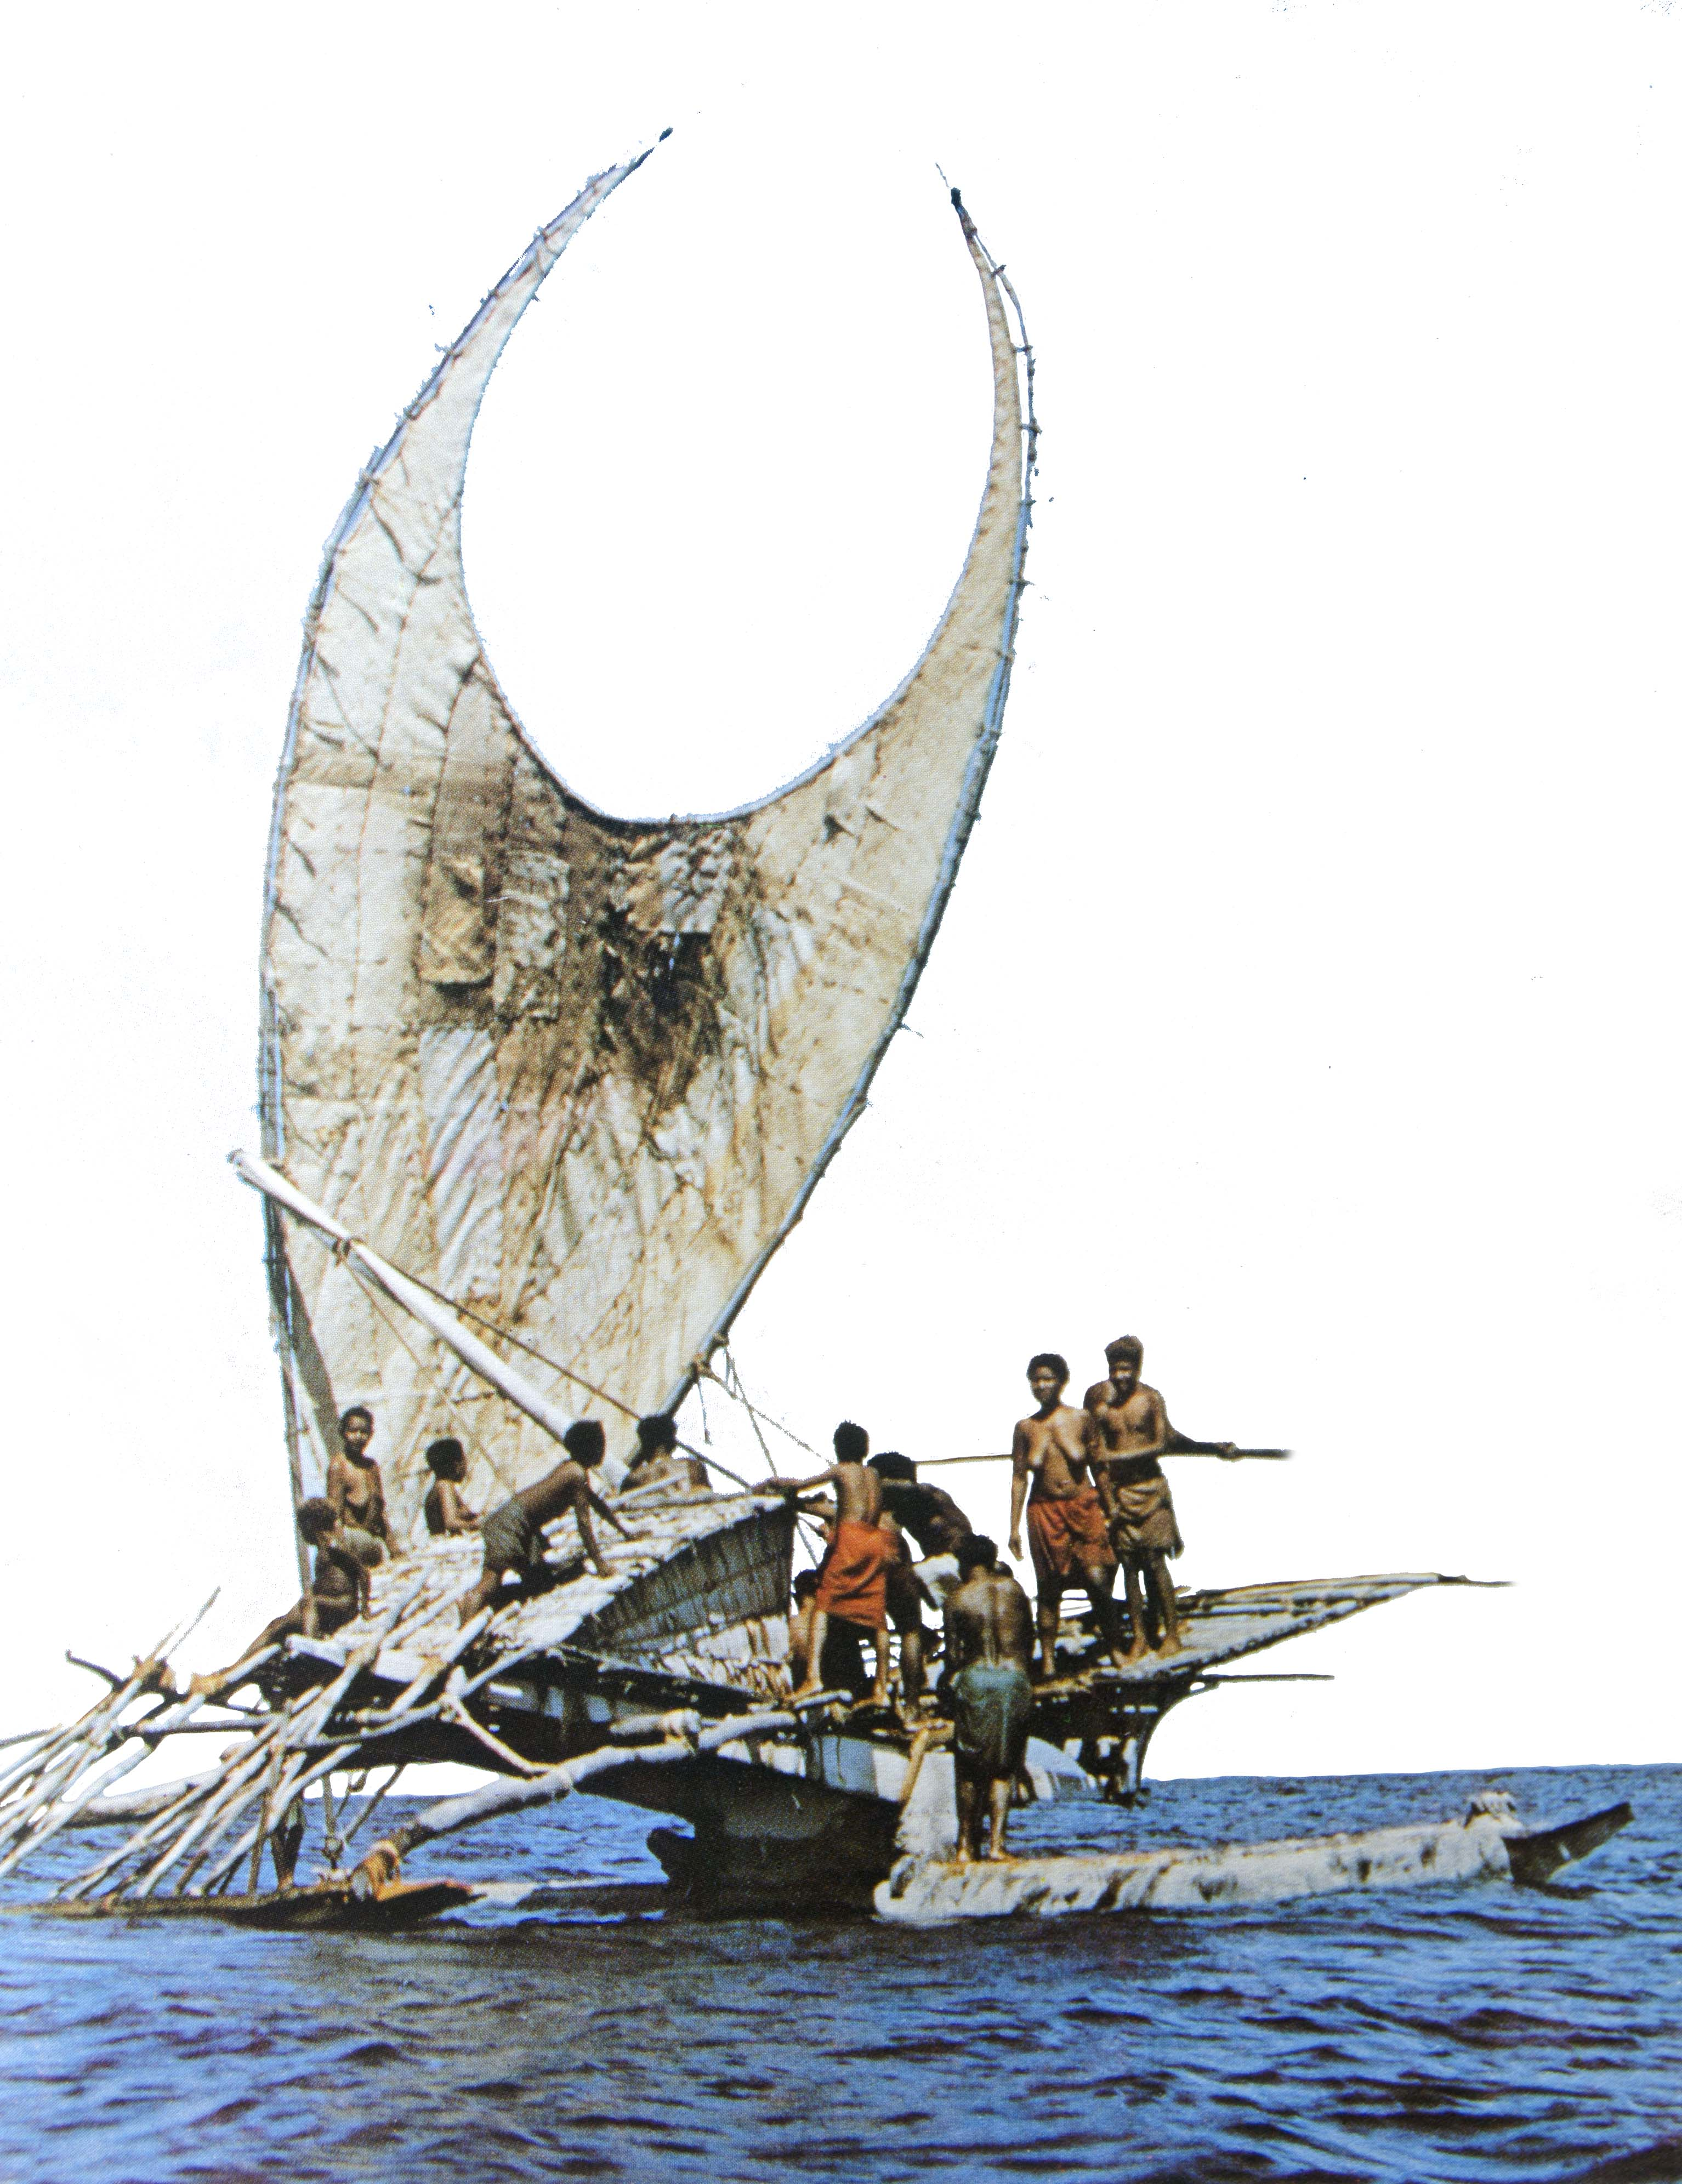
\includegraphics[width=\linewidth]{static/tonga_barco.jpg}
  \caption{}
  \label{fig:tecnologia}
  \end{subfigure}
 \caption{
(\subref{fig:poblamiento}): Poblamiento del mundo (flechas) y desarrollo independiente de la agricultura (puntos) en una proyección del mapamundi que preserva los tamaños relativos de los continentes. (\subref{fig:pacifico}): El aumento de la población hace de los centros agrícolas regiones ricas en innovaciones tecnológicas, y para el año 1300 ya se habían producido intercambios entre el Pacífico y América del sur. (\subref{fig:tecnologia}): Imagen de la extraordinaria tecnología de navegación utilizada en el Pacífico.
 }
 \label{fig:desert}
 \end{figure}


% Parrafo


% Durante el a\~no 1400 el mundo florec\'ia de sociedades ``pr\'osperas''~\cite{dussel2004-sistemaMundo}.
% %
% %El desarrollo tecnol\'ogico de todas estas sociedades fue extraordinario.
% %
% % El imperio de Tonga ocupaba hace siglos todo el oc\'eano Pac\'ifico (figura~\ref{fig:polynesia}) con tecnolog\'ias de navegaci\'on que le hab\'ian permitido tener intercambios con Am\'erica de Sur~\cite{thorsby2016-polynesiaAmerica, ioannidis2020-polynesiaAmerica}.
% % %
% % En Am\'erica del Sur se hab\'ia desarrollado un sistema de intercambios basado en la reciprocidad de trabajo (minka, ayni y mita) que le permit\'ia a las comunidades administrar eficientemente el uso de los bienes comunes y al Estado desarrollar la infrastructura en el vasto territorio monta\~noso~\cite{murra1978-organizacion}.
% % %
% % En la regi\'on Azteca se hab\'ia desarrollado un extenso mercado regional con ciudades de hasta 300.000 habitantes, tres veces la ciudad de Venecia en esa misma \'epoca.%~\cite{www7.uc.cl}. %http://www7.uc.cl/sw_educ/historia/conquista/parte1/html/h54.html
% % %
% % El mundo \'Arabe comerciaba productos desde el Oc\'eano Pac\'ifico, en las Filipinas, hasta el Oc\'eano Atl\'antico, en Marruecos, conectando las innovaciones culturales de distintos hemisferios del planeta~\cite{dussel2004-sistemaMundo}.
% % %
% África siempre fue el continente m\'as diverso cultural y gen\'eticamente, pero quiz\'as el centro m\'as innovador en t\'erminos cient\'ificos y tecnolog\'ias haya sido la regi\'on de China~\cite{needham2004-generalConclusionsAndReflections}.


Para el año 1400 el mundo florecían de sociedades prósperas.
%
En el mundo Árabe se comerciaban productos desde el océano Atlántico en España, hasta el océano Pacífico en las Filipinas.
%
El océano Pacífico estaba totalmente ocupado, y ya se habían producido intercambios entre Oceanía y América del Sur, que se refleja en la genética de las poblaciones actuales \cite{ioannidis2020-polynesiaAmerica} (figura~\ref{fig:pacifico}).
%
Y en el jardín de la diversidad genética y cultural humana, África subsahariana, se desarrollaba entre otras, la sociedad Bantu.
%
Pero China era para ese entonces el principal centro productivo y tecnológico del mundo después de 2 milenios.

% Parrafo

John Needham, el brit\'anico que dedic\'o su vida a recopilar la monumental historia cient\'ifica y t\'ecnica de China, reconoce que comenz\'o a estudiar el tema motivado por responder la pregunta de por qu\'e s\'olo Europa occidental hab\'ia logrado el avance cient\'ifico.
%
\begin{quotation}
When I first formed the idea, about 1938, (...) I regarded the essential problem as that of why modern science had not developed in Chinese civilisation (or Indian or Islamic) but only in that of Europe~\cite{needham2004-generalConclusionsAndReflections}.%
\end{quotation}
Luego de 60 a\~nos de investigaciones, Needham se ve obligado inviertir la pregunta.
\begin{quotation}
Why, between the -1th century and the 15th century, was Chinese civilisation much \emph{more} efficient than occidental in gaining natural knowledge and in applying it to practical human needs?~\cite{needham2004-generalConclusionsAndReflections}
\end{quotation}

% Parrafo

Desde Hegel hasta la fecha, las explicaciones euroc\'entricas intentan explicar la prosperidad actual de occidente a trav\'es de una causa interna: la ``\'etica protestante'' de Max Weber~\cite{weber1905-eticaProtestante}, la ``mentalidad burguesa'' de Jos\'e Luis Romero~\cite{romero1967-revolucionBurguesa}, o m\'as recientemente el ``sistema de parentesco'' de Joseph Henrich~\cite{henrich2020-weirdest}.
%
La paradoja que no puede responder es c\'omo una sociedad sumida en un proceso de involuci\'on cultural \'unico, como la sociedad feudal de la ``edad media'', pudo generar de repente el extraordinario proceso de desarrollo cient\'ifico y t\'ecnico de la modernidad.

\subsection{Coyuntura colonial-moderna}

As\'i como la cooperación favorece los proceso de innovaci\'on y acumulaci\'on cultural, el aislamiento está asociado a p\'erdidas masivas de informaci\'on cultural.
%
El ejemplo más paradigm\'atico es el aislamiento total que ocurrió con la separaci\'on de Tasmania del continente Australiano por la subida del nivel del mar a comienzos del Holonceno.
%
\begin{figure}[ht!]
  \centering
  \begin{subfigure}[c]{0.42\textwidth}
    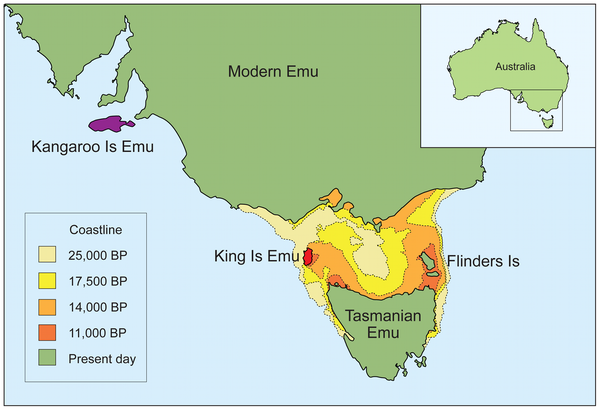
\includegraphics[width=\textwidth]{static/tasmania.png}
    \caption{Tasmania}
    \label{fig:tasmania}
  \end{subfigure}
%   \begin{subfigure}[c]{0.45\textwidth}
%     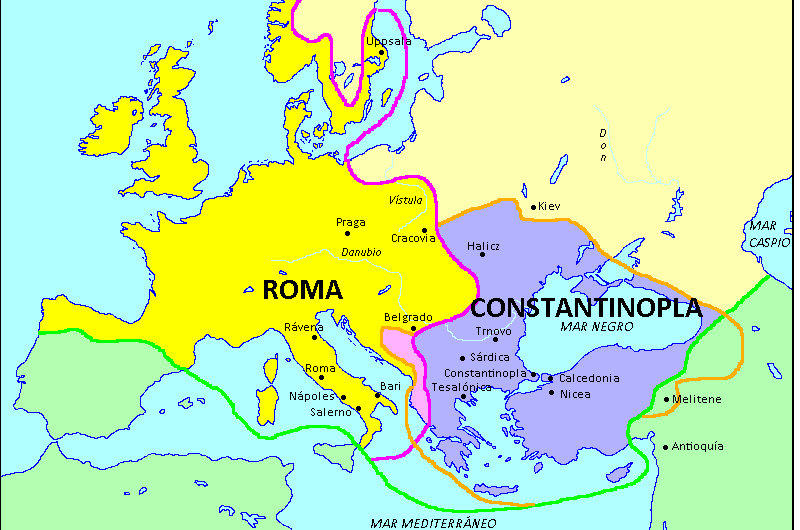
\includegraphics[width=\textwidth]{static/cisma.png}
%     \caption{Edad media}
%     \label{fig:cisma}
%   \end{subfigure}
  \caption{Ejemplo paradigmático de aislamiento e involución cultural}
  \label{fig:aislamiento}
\end{figure}
La evidencia indica que las sociedades que permanecieron en la isla de Tasmania perdieron gran parte de su cultura tecnol\'ogica.
%
La principal hip\'otesis sugiere que la reducci\'on del tama\~no efectivo de la poblaci\'on fue la causa de la p\'erdida cultural~\cite{Henrich2004}.
%
La capacidad de almacenamiento (e innovaci\'on) de tecnolog\'ias complejas requerir\'ia un tama\~no m\'inimo de la poblaci\'on, incluso en sociedades cazadoras-recolectoras.

% Parrafo

De forma similar, la masiva destrucción de la diversidad cultural al interior del imperio Romano y el conflicto permanente con las sociedades vecinas, generó el aislamiento parcial de Europa occidental del sistema mundo, conduciéndola a contramano del resto del mundo a un largo proceso de involución cultural y de violencia interna conocido como ``Edad media''.
%
% Arrinconada ya en el lejano occidente por el fr\'io polar al norte y la falta de tecnolog\'ias para navegar las aguas del oeste, Europa occidental comienza en el siglo octavo a quedar paulatinamente aislada del ``sistema mundo'' por la expansi\'on Árabe al sur y por la serie cismas con el Imperio Romano de Oriente~\cite{Dussel}.
%
% %
% Aislada parcialmente del sistema mundo, esta sociedad entra en un proceso de involuci\'on cultural que condujo a un deterioro extremo de las condiciones de vida.
En esta etapa, se generalizó al interior de la sociedad feudal el criterio de autoridad como fundamento del ``saber auténtico''.
%
Un nuevo sistema penal, sin límites, renació de los llamados \emph{libris terribilis} y las instituciones heredadas del imperio Romano de occidente comenzaron a regular las relaciones comunitaria de reproducción sexual de forma más detallada que la propiedad privada.
%
La guerra contra las mujeres se formaliza con la publicación del \emph{Malleus maleficarum} en 1484 (caza de brujas), que será el segundo best seller después de la Biblia durante los siguientes 200 años en Europa occidental~\cite{zaffaroni2013-cuestionCriminal}.


% Parrafo

Aunque exista una desventaja evolutiva de la deserción, ciertas coyunturas pueden producir su emergencia en el corto plazo (\emph{propiedad menor}).
%
Así es que la coincidencia de un conjunto de eventos, que se desencadenaron por la masiva migración feudal a América, puso de repente a esa sociedad, históricamente marginal, en una situación de privilegio mundial.
%
Las enfermedades transmitidas por los exploradores feudales eliminó, al menos, a 2/3 de la población americana.
%
Sin embargo, no se produce ningún giro geopolítico hasta que en 1546 los exploradores feudales descubren la montaña de plata de Potosí, metal que China había incorporado recientemente como una de sus monedas oficiales.
%
Gracias a ella, un cuarto de siglo después, Europa occidental comienza a romper su aislamiento (batalla de Lepanto 1571) y dar inicio a un largo ciclo de importación de tecnología extranjera, principalmente China.

% Parrafo

Cuando la sociedad feudal empieza a adquirir una posición de privilegio en el sistema mundo, comienza al interior de esta sociedad un nuevo debate sobre las fuentes de validación del conocimiento.
%
En esta época, el criterio de autoridad de la Edad Media como fundamento del saber auténtico comienza a ser reemplazado por los criterios de experiencia personal.
%
Algunos entendieron el concepto de experiencia como ``evidencia intelectual'' (racionalistas) y otros como ``evidencia sensible'' (empiristas), dos grupos de exigencias que se consideraron al principio incompatibles entre sí: el de universalidad y necesariedad por un lado, y el de acreditación empírica por otro~\cite{samaja1999-epistemologiaYMetodologia}.

% Parrafo

Al mismo tiempo, la posición de privilegio mundial permitió a la sociedad feudal trasladar parte de su estructura de dominación afuera de su frontera.
%
El argumento de superioridad moral que será empleado durante toda la colonial-modernidad hasta el presente, lo desarrolla por primera vez Ginés de Sepúlveda justo cuatro años después del descubrimiento de la plata de Potosí~\cite{dussel2020-primerDebate}.
%
\begin{quotation}
 Será siempre justo [...] que tales gentes [bárbaras] se sometan al imperio de príncipes y naciones más cultas y humanas [...] Y si rechazan tal imperio se les puede imponer por medio de las armas, y tal guerra será justa según el derecho natural lo declara [...] En suma: es justo, conveniente y conforme a la ley natural que los varones probos, inteligentes, virtuosos y humanos dominen sobre todos los que no tienen estas cualidades.%~\cite{GinesdeSepulveda1967p87}.
\end{quotation}
%
El sujeto masculino blanco se coloca a sí mismo como modelo del interés general y valor universal, reduciendo al resto de los seres vivos a meros objetos de uso.
%
La sociedad colonial-moderna, y su ciencia, repite la estructura verticalista y punitivista de la sociedad feudal, ahora con un alcance global.
%
Todos los conocimientos que la nueva sociedad colonial-moderna va incorporando del resto de comunidades del mundo se les borra su verdadero origen histórico y se las enaltecen como surgimientos espontáneos internos~\cite{dussel1992-encubrimiento}.

% Parrafo

La plata de Am\'erica fluy\'o en todas las direcciones, principalmente hacia China.
% %
Más de dos siglos después del acceso a la plata americana, Europa occidental segu\'ia consumiendo más productos asi\'aticos de los que pod\'ia exportar a Asia.
% %
% El comercio internacional de opio comenz\'o como respuesta a una crisis del comercio internacional europeo, especialmente brit\'anico.
% %
Todavía a comienzos del 1800 Europa occidental seguía teniendo déficit comercial con China, que desde mediados de 1700 financiaba mediante el narcotráfico de opio a pesar de la prohibición China.
%
El opio, un producto lujoso utilizado en China como medicina (raramente como estupefaciente), fue prohibido por los emperadores chinos en 1729 debido a que su abundancia hac\'ia crecer lentamente la cantidad de adictos~\cite{pomeranz2018-tradeCreated}.
%
Las consecuencias fueron más graves cuando, después de las independiencias americanas, en 1818, los británicos comienzan a comercializar una mezcla de opio más barata y potente.
%
El número de adictos llegó a ser lo suficientemente alarmante, y en 1839 China comete el error de declarar la guerra al Narco-Estado británico en su propio territorio.
%
Los resultados fueron terribles: China pierde 1/5 de su población y queda sumida durante un siglo por invasiones extranjeras.

\begin{figure}[ht!]
\centering
 \begin{subfigure}[b]{0.45\textwidth} \centering
  \includegraphics[width=\linewidth]{figures/china.pdf}
  \caption{}
  \label{fig:china}
  \end{subfigure}
  \begin{subfigure}[b]{0.27\textwidth} \centering
  \includegraphics[width=\linewidth]{static/africa.png}
  \caption{}
  \label{fig:africa}
  \end{subfigure}
 \caption{
 \en{(\subref{fig:china}): China's defeat against the British narco-state on its own territory had terrible consequences. (\subref{fig:africa}): It was not until 1850 that the colonization of continental Africa and the vast territories of the still autonomous Americas began.}%
 \es{(\subref{fig:china}): La derrota de China contra el narco-estado británico en su propio territorio tuvo consecuencias terribles. (\subref{fig:africa}): Recién a partir de 1850 comienza la colonización de África continental y los extensos territorios de América todavía autónomos.}%
 }
 \label{fig:eraDeGenocidios}
 \end{figure}

% Cuando Europa occidental finalmente se establece como el centro geopolítico global, luego de la derrota China, comienza la era de genocidios y masiva pérdida de diversidad cultural global: la ocupación violenta de África continental y de los territorios de América todavía autónomos, entre los principales.
%
Luego de la derrota de China por parte del narco-estado brit\'anico, se establece por primera vez la hegemon\'ia de Europa occidental en el sistema mundo y comienza el proceso de colonizaci\'on de África continental y de los extensos territorios americanos que todav\'ia segu\'ian en manos de comunidades locales, entre los principales.
%
Comienza la era de genocidios.
%
En todas las partes del globo, los exploradores y etn\'ografos fueron documentando la perdida completa de culturas debida al avance del frente colonial-moderno, estatal o privado, sobre las autonom\'ias locales.
% %
Es una época de avances cient\'ificos y tecnol\'ogicos por un lado, pero es al mismo tiempo la era masiva pérdida de diversidad cultural global.
%
% El criterio de autoridad globalizado durante la colonial-modernidad como criterio de universalidad limitado a los varones blancos abrió la puerta a la arbitrariedad cultural y ecológica.
%
%
En un mundo de comunidades debilitadas, se expande la cosmovisión individualista e instrumental de nuestro tiempo, la naturaleza como cosa, las personas como cosas, y se desencadena así la masiva p\'erdida de biodiversidad actual.

% Parrafo

La ventaja a favor de la diversificación y la cooperación no es solo teórica, su ruptura tiene consecuencia para la vida y el conocimiento.
%
A pesar de todos los avances, la ciencia metropolitana no fue capaz de compensar la pérdida de conocimientos milenarios provocada por la colonial-modernidad, y como consecuencia de la masiva pérdida de la diversidad cultural global vivimos en la actualidad una grave crisis ecológica que no deja de profundizarse.
% El remplazo repentino de estos sistemas culturales locales por instituciones externas, estatales o de mercado, que exhiben lógicas ``singulares y definitvas'', ha producido devastadoras consecuencias culturales y ecológicas~\cite{segato2013-colonialidad}.
% % %
Del mismo modo que seleccionar una única hipótesis tiene consecuencias negativas conocidas en probabilidad (overfitting), la imposición de un único tipo de sociedad ha mostrado tener consecuencia ecológicas cada vez más negativas.

% Parrafo

Los estudios comparados muestran que las instituciones humanas capaces de administrar exitosamente los bienes comunes y establecer relaciones de largo plazo con los sistemas ecológicos emergen en comunidades autónomas con fuerte arraigo local.
%
Por ello es indispensable una coexistencia intercomunitaria que reconozca las autonomías jurisdiccionales locales, para que cada pueblo pueda desarrollar, a lo largo de su historia, su propio ordenamiento normativo, cultural y político.

\section{Objetivos}

% Parrafo: El objetivo subyacente de esta tesis. Interdisciplina entre la computación y las ciencias sociales.


No toda verdad es igualmente relevante.
%
Los problemas de conocimiento están, directamente o indirectamente, en función de un conjunto de problemas reales, y de ellos obtiene su relevancia y jerarquía.
%
Si bien los problemas científicos suelen exprese sólo en relación a sus aspectos teóricos, es de gran importancia poner al descubierto el sistema de relaciones que conducen hasta su base real.
%
%El concepto mismo de ``problema'' sólo adquiere sentido en relación a alg\'un sistema vivo.
%
Los problemas de la física y la química existen en tanto se subsumen como relevantes para la reproducción de la vida, ligada a un contexto histórico y evolutivo.
%
El modo de formular los problemas orienta desde el origen el tipo de preguntas, los datos que se seleccionan, los modelos causales que se consideran, y por lo tanto el espacio posible de respuestas.
%
Por lo tanto, examinar los contextos constituye una tarea decisiva para determinar la relevancia de los problemas de conocimiento.

% Parrafo

El objeto de estudio que motivó el plan fue entender el comportamiento del la cultura humana: un sistemas natural de procesamiento distribuido de información.
%
Debido a que la cultura es un fen\'omeno poblacional que emerge como consecuencia del intercambio de informaci\'on entre individuos, en esta tesis nos propusimos estudiar el efecto que las interacciones sociales (su contexto, dinámica y estructura) tiene sobre el aprendizaje individual.

% Parrafo

Entender cómo cambia la cultura en el tiempo no solo es uno de los problemas fundamentales de la antropología, es también uno de los problemas que las ciencias de la computación deberá responder en los próximos años.
%
En los últimos años las empresas Deep Mind y Meta abrieron nuevas líneas de investigación en lo que se ha dado a llamar \emph{cooperative AI}~\cite{dafoe2020-coopAI, dafoe2021-coopAIcomment}.
%
Solo recién durante la escritura de esta tesis, han comenzado a surgir los primeros resultados de nivel humano en un juego de estrategia ``Diplomacy'', que involucra negociación entre varios jugadores~\cite{kramar2022-deepMindDiplomacy, meta2022-diplomacy}
%
Sin embargo, todavía no ha madurado lo suficiente la inteligencia artificial multi-agente, que permitiría comprender el comportamiento de los sistemas de culturales.

% Parrafo

Hasta ahora, las respuestas con mayor influencia se han propuesto a través de modelos matemáticos de evolución cultural.
%
Basada en los principios de la teor\'ia de la evoluci\'on (descendencia, modificaci\'on y selecci\'on), se ha desarrollado un marco te\'orico de \emph{evoluci\'on cultural} que intenta explicar c\'omo cambia la cultura en el tiempo~\cite{boyd1985-evolutionaryProcess, boyd2005-origin}.
%
Ella no es más que una aplicación de la teoría de juegos evolucionaria \cite{taylor1978-replicatorDynamic, maynardSmith1982-evolutionGameTheory}, que modela los equilibrios evolutivos que se producen entre estrategias en competencia, en el que la adaptabilidad de cada variante depende de las frecuencias de las otras variantes en la población.
%
%Estos trabajos son, esencialmente, modelos teóricos destinados a comprender las consecuencias que ciertas relaciones causales podrían tener en fenómenos naturales en caso de que sus estructuras sean análogas.
%
%Este es un abordaje útil para ganar intuición de procesos complejos, como son las propiedades que emergen en los sistemas a partir de la interacción de sus partes.
%
Si bien estos modelos sirven para ganar intuición de procesos complejos, sus resultados son analogías que no están destinadas a realizar predicciones y por lo tanto poseen una débil corroboración empírica.

% Parrafo

Esta es una tesis interdisciplinaria que, desde su concepción, ha tenido como objetivo sacar provecho de la relación entre las ciencias de la computación y las ciencias sociales.
%
Durante el transcurso del doctorado emergió con fuerza una área conocida como Ciencias Sociales Computacionales~\cite{lazer2009-computationalSocialScience, lazer2020-computationalSocialScience}, que tiene en la actualidad reconocimiento tanto en institutos de primer nivel de ciencias de la computación como en los gigantes tecnológicos relacionados a la industria del software.
%
%Bajo esta categoría quedaron enmarcadas una gran variedad de actividades, a veces bastante diferentes entre sí, desde aquellas que usan la computación como una herramienta para analizar datos de origen sociales, hasta aquellas que usan problemas de ciencias sociales para motivar desarrollos en la frontera del conocimiento en las ciencias de la computación~\cite{lazer2020-computationalSocialScience}.
%
%Pero la emergencia de la interdisciplina es un fenómeno más general.
%
En la última década, las ciencias de la computación han tenido un impacto profundo en casi todas las disciplinas científicas.%, impulsadas por los avances en el área de la inteligencia artificial y la masificación datos y métodos de aprendizaje automático.
%
Una de sus consecuencias más contundentes es la emergencia e institucionalización de la Ciencia de Datos, un área científica que ha nacido interdisciplinaria por definición.

% Parrafo

En nuestro contexto, decidimos enfocarnos en el análisis del comportamiento de los individuos en comunidades de video juegos en línea.
%
Si bien las comunidades virtuales determina el contexto de los actos y limitan el conjunto de acciones y se\~nales que las personas pueden ejecutar, ellas ofrecen nuevos horizontes en la investigaci\'on cient\'ifica sobre comportamientos sociales pues re\'unen al mismo tiempo la posibilidad de estudiar poblaciones suficientemente grandes con un alto grado de detalle.
%
En particular, los videojuegos aparecen como un lugar privilegiado para estudiar cómo cambian las estrategias en el tiempo en un escenario social relativamente simplificado, donde las reglas se mantienen estables.
%
Ninguna de las metodolog\'ias cl\'asicas de las ciencias sociales (censo, encuesta, etnograf\'ia) ofrecen simult\'aneamente ambos niveles de análisis.

% Parrafo

En la última década se a producido una enorme cantidad de investigaciones sobre comportamientos humanos basados en comunidades virtuales.
%
En particular, esta ha sido una línea de investigación exitosa de mi co-director Diego Fernández Slezak~\cite{slezak2012-doNotFearYourOpponent} quien estudió el efecto del miedo en una base de datos de ajedrez rápido.
%
Además, la comunidad de evolución cultural ha estado especialmente interesada en este campo.
%
Por ejemplo, Bret Beheim~\cite{Beheim2014} pone a prueba las predicciones sobre los tipos de estrategias de aprendizaje social, así como la poblacional, analizando los movimientos de apertura de los jugadores profesionales del juego de Go.
%
Otro ejemplo, Elena Miu~\cite{miu2018-cumulativeCultureOnlineProgrammingContests} estudió la dinámica de acumulación cultural en competencias de programación en línea.
%
Otros trabajos estudian aspectos relacionales a la evolución cultural en las letras de canciones pop \cite{brand2019-songLyrics} y las estrategias del football~\cite{mesoudi2020-footballTactics}.

% Parrafo

El plan de tesis tiene como objetivo particular poner a prueba algunas de las hipótesis propuestas por los modelos te\'oricos, evaluándolas en los datos generados por comunidades virtuales de juegos en l\'inea multijugador de tipo estrat\'egico de mediana y larga duraci\'on.
%
Conocer c\'omo las personas aprendemos es un problema importante para muchos \'ambitos de la vida, como la educaci\'on, el trabajo y el deporte.
%
En general las investigaciones se han enfocado principalmente en los factores cognitivos individuales del aprendizaje.
%
Esta tesis estudia el impacto que ciertos factores sociales que afectan el aprendizaje individual esperado por el simple experiencia individual.
%
¿Cuál es la relaci\'on entre la formación de equipos y el aprendizaje individual a largo plazo?
%
¿Cuál es la mejor forma de medir el aprendizaje de un individuo en el tiempo?
%
¿Cu\'al es el efecto que la posici\'on topol\'ogica de un individuo en la red de intercambios dinámica tiene sobre el aprendizaje individual?

% Parrafo

El plan utiliza metodologías computacionales e informáticas para evaluar estas y otras hipótesis en base a los datos.
%
Las reglas de la probabilidad se conocen desde finales del siglo 18 y desde entonces se las ha adoptado como sistema de razonamiento en todas las ciencias con datos.
%
Sin embargo, la aplicación estricta de las reglas de la probabilidad (enfoque bayesiano) ha estado históricamente limitada debido al costo computacional asociado a la evaluación de todo el espacio de hipótesis.
%
Solo recientemente, luego de que se produce el enorme crecimiento en la capacidad de cómputo, comienza por primera vez a ser posible computar la incertidumbre óptima dada la información disponible en todos los campos de la ciencia.

\subsection{Estructura de la tesis}

Los resultados de esta tesis están ordenados siguiendo el recorrido temporal.
%
En el capítulo \ref{} se presenta la metodología bayesiana y el estimador de habilidad bayesiano más utilizado en la industria del video juego al inicio de esta tésis.
%
En el capítulo \ref{} reportamos el primer resultado, donde usamos ese estimador bayesiano de habilidad para estudiar una comunidad en el que las personas podían jugar individualmente o en equipos.
%
Allí encontramos que jugar en equipo está asociado a mayor aprendizaje a largo plazo, y que mantener un equipo estable está asociado a mayor velocidad de aprendizaje.
%
En el capítulo \ref{} implementamos el modelo de habilidad estado del arte (disponible hoy en Julia, Python y R) que, al propagar correctamente la información histórica en una única red causal, es capaz de proporcionar estimaciones con baja incertidumbre en todo momento, asegurando la comparabilidad en el tiempo y el espacio.
%
En el capítulo \ref{} reportamos el tercer resultado, donde estudiamos la evolución de una red de partidas en el juego de Go durante un periodo de ocho años.
%
Allí encontramos, con el nuevo estimador, que la posici\'on de los individuos en la red tiene un efecto de segundo orden sobre el aprendizaje en los personas que están en el medio del proceso de aprendizaje, ausente entre novatas y expertas.





















































\chapter{Metodología: incertidumbre e información.}


% La ciencia es una institución que tiene pretensión de verdad: alcanzar acuerdos intersubjetivos con validez universal.
% %
% Las ciencias formales (matemática, lógica) alcanzan estos acuerdos derivando teoremas dentro de sistemas axiomáticos cerrados.
% %
% Sin embargo, las ciencias empíricas (desde la física hasta las ciencias sociales) deben validar sus proposiciones en sistemas abiertos que contienen siempre algún grado de incertidumbre.
% %
% ¿Es posible entonces alcanzar acuerdos intersubjetivos ("verdades") en las ciencias empíricas en las que es inevitable decir "no sé"? Sí.
% %
% Podemos evitar mentir: maximizando incertidumbre (no afirmar más de lo que se sabe) dada la información disponible (sin ocultar lo que sí se sabe)~\cite{Jaynes2003}.

% Parrafo

Las reglas de la probabilidad se conocen desde finales del siglo 18 y desde entonces se las ha adoptado como sistema de razonamiento en todas las ciencias empíricas.
%
Estas reglas son conceptualmente intuitivas: preservar la creencia previa que sigue siendo compatible con los datos (regla del producto) y predecir con la contribución de todas las hipótesis (regla de la suma).
%
A lo largo de todos estos siglos, las reglas de la probabilidad han sido derivadas repetidas veces a partir de diversos sistemas axiom\'aticos~\cite{halpern2017}.
%
Si bien en todo este tiempo no se ha propuesto nada mejor en términos prácticos, el costo computacional asociados a la evaluación de todo el espacio de hipótesis ha limitado históricamente la aplicación estricta de las reglas de la probabilidad.
%
Por ello, a lo largo de los siglos se fueron desarrollando técnicas para resolver este problema.

% Parrafo

El primer ciclo de soluciones llega de la mano de física estadística, en la segunda mitad del siglo 19.
%
En esta época se desarrollan métodos analíticos para estimar la probabilidad de los microestados dada alguna información macro, como la energía, la temperatura, o algún promedio.
%
Conceptualmente se ha mostrado que las soluciones que ofrece la física estadística son equivalentes a las que se obtiene con el enfoque bayesiano a través del principio de ``no mentir'' (maximizar entropía dada la información disponible)~\cite{jaynes1957-informationTheoryAndStatisticalMechanics, jaynes2003-bookProbabilityTheory}.

% Parrafo

Durante el siglo 20 se deja de lado la pretensión de evaluar todo el espacio de hipótesis y se comienzan a desarrollar métodos que seleccionan una única hipótesis mediante alguna función de costo ad-hoc (e.g~como máxima verosimilitud).
%
Estas aproximaciones puntuales, al evitar evaluar todo el espacio de hipótesis, permitieron en la práctica extender el campo de aplicaciones de la teoría de la probabilidad~\cite{friedman2001-elementsOfStatisticalLearning}.
%
Sin embargo, debido a que las técnicas de selección de hipótesis puntuales muestra todavía inestabilidades (e.g.~overfitting), buena parte del trabajo durante esta época estuvo dedicado a desarrollar métodos robustos.

% Parrafo

En las vísperas del siglo 21, el crecimiento en la capacidad de cómputo levantó finalmente el principal obstáculo que pesaba sobre la aplicabilidad de las reglas de la probabilidad.
%
En esta época se desarrollan los métodos numéricos de aproximación por muestreo (basados en Cadenas de Markov) y los métodos analíticos basados en minimización de divergencias entre distribuciones de probabilidad~\cite{bishop2006-PRML}.
%
Por primera vez desde el descubrimiento de la teoría de la probabilidad, comienza a ser posible en todos los campos de las ciencia resolver la inferencia de los modelos probabilísticos aplicando estrictamente las reglas de la probabilidad, evaluando todo el espacio de hipótesis (aka~enfoque bayesiano).

% Parrafo

Si bien en la actualidad el crecimiento del enfoque bayesiano es un fenómeno mundial que se está acelerando, su desarrollo sigue siendo incipiente.
%
Luego de superados estos obstáculos, la inercia histórica aparece ahora como una de las limitaciones principales, a la que nuestra casa de estudios no está exenta.
%
Por ello, antes de presentar los modelos básicos de estimación de habilidad, introducimos los fundamentos epistemológicos de la construcción de conocimiento en contextos de incertidumbre (secci\'on \ref{sec:principios_interculturales}), y revisamos el enfoque bayesiano de la probabilidad (seccón \ref{sec:reglas_de_la_probabilidad}).

% Parrafo

La evaluación de modelos causales alternativos y la construcción de datos son dos tareas centrales a resolver en ciencias emp\'iricas.
%
Los métodos frecuentistas no ofrecen soluciones a estos dos problemas.
%
Por ello, mostraremos cómo la aplicación estricta de las reglas de la probabilidad permiten: evaluar naturalmente modelos causales alternativos (secci\'on \ref{sec:modelos_alternativos}); y construir sistemas de información óptimos (datos) que sirvan como base emp\'irica para evaluar nuevas hip\'otesis (secci\'on \ref{sec:base_empirica_metodo}).
% Parrafo
En la sección \ref{sec:trueskill} mostramos en detalle el modelo de estimación de habilidad bayesiano más utilizados en el industria del video juego.
%que utilizaremos para construir base empírica en uno de nuestros trabajos, y que evalupara aanlizar los factores de aprendizaje social el siguiente capítulo.
%

%

\section{Razonamiento bajo incertidumbre}\label{sec:principios_interculturales}

Las reglas de la probabilidad constituyen el principal sistema de razonamiento bajo incertidumbre.
%
Estas reglas puede derivarse de principios filos\'oficos con validez intercultural.
%
El ``principio de integridad'' garantiza que no exista ni p\'erdida ni creaci\'on espontánea de creencias cuando la distribuimos entre las hip\'otesis alternativas.
%
El ``principio de no mentir'' garantiza un primer acuerdo intersubjetivo en contextos de incertidumbre (máxima incertidumbre dada informaci\'on disponible).
%
Finalmente, el ``principio de coherencia'' garantiza la continuidad del acuerdo intersubjetivo mediante la preservaci\'on de la creencia que sigue siendo compatible con los datos de base emp\'irica.

\subsection{Incertidumbre}

La idea de que \emph{todo} lo que ocurre en la naturaleza tiene una causa previa que lo genera se conoce en la historia de la filosof\'ia como el principio de \emph{raz\'on suficiente} y ha estado presente en los debates que anteceden el desarrollo de la teoría de la probabilidad.
%
%Leibniz (1646-1716),  \cite{Leibniz and China: A Commerce of Light}
%La Monadolog\'ia (escrita en franc\'es en 1714 y publicada en alem\'an en 1720)  \cite{leibniz1714-monadologie}.
%
Esta idea parece está relacionada con la imposibilidad de crear azar, de crear un ``método efectivo'' capaz de generar a veces un resultado y a veces otro dadas exactamente las mismas condiciones iniciales.
%
Antes del desarrollo de las ciencias de la computación existía una intuición respecto de su imposibilidad.

% Parrafo

En teor\'ia de la computabilidad, la tesis de Church-Turing afirma que toda funci\'on sobre los n\'umeros naturales puede ser calculada por un ``m\'etodo efectivo'' si y s\'olo si es computable por una m\'aquina de Turing.
%
Debido a que todos las definiciones alternativas del concepto de ``m\'etodo efectivo'' resultaron ser equivalentes a una maquina de Turing, actualmente se supone que la hip\'otesis Church-Turing es cierta.
%
La imposibilidad de crear números aleatorios está determinada por la definición misma de función, $f(x) = y$, pues las mismas condiciones iniciales $x$, luego de aplicado un ``método efectivo'' $f$, debe producir siempre el mismo resultado $y$.

% Parrafo

El fundador de la teoría de la probabilidad moderna, Pierre-Simon Laplace (1749-1827), ten\'ia la convicci\'on de que no existían eventos aleatorios en la naturaleza.
%
Que si tuviéramos conocimiento completo (infinitamente preciso) del estado del mundo $x$ en un instante de tiempo, y el modelo causal correcto que rige el comportamiento del mundo $f$, entonces tendr\'iamos conocimiento completo del estado del mundo en cualquier instante posterior $y$.

\begin{quotation}
Les événemens actuels ont, avec les précédens, une liaison fondée sur le principe évident, qu’une chose ne peut pas commencer d’être, sans une cause qui la produise. [\dots] Une intelligence qui, pour un instant donné, connaîtrait toutes les forces dont la nature est animée [\dots] rien ne serait incertain pour elle, et l’avenir comme le passé, serait présent à ses yeux~\cite{laplace1816-philosophique}. \end{quotation}

Vivir en un mundo determinista no nos libera, sin embargo, de la incertidumbre.
%
Conocer las condiciones iniciales con precisi\'on \emph{finita} ha mostrado ser suficiente para impedir predecir el comportamiento de modelos causales, incluso en el corto plazo.
%
Un ejemplo de sistema determinista capaz de adquirir comportamientos imprevisibles es el siguiente modelo ``poblacional''.
%
\begin{equation}
 \text{Poblaci\'on}(t+1) = r \cdot \text{Poblaci\'on}(t)\cdot (1-\text{Poblaci\'on}(t))
\end{equation}
%
El modelo establece que el tama\~no de una poblaci\'on, medida como proporci\'on respecto de la capacidad m\'axima de un sistema, depende exclusivamente de su tama\~no en el tiempo anterior y de un factor de reproducci\'on $r$.
%
Las relaciones causales se suelen expresar en t\'erminos gr\'aficos.

% Parrafo

\begin{figure}[ht!]
\centering
\tikz{
    \node[latent, minimum size=1.25cm] (n1) {$\text{pob}_n$} ;

    \node[latent, right=of n1, xshift=3cm, minimum size=1.25cm] (n2) {$\text{pob}_{n+1}$} ;

     \path[->] (n1) edge node [yshift=0.5cm] {$r \cdot \text{pob}_n \cdot (1-\text{pob}_n)$} (n2);

}
\caption{Modelo causal expresado gr\'aficamente. Las flechas representan la relaci\'on causal entre las variables. }
\label{fig:modelo_poblacional}
\end{figure}

% Parrafo

Dependiendo del factor de reproducci\'on $r$ y de la poblaci\'on inicial pop$_0$, podemos observar diferentes tipos de comportamientos.
%
Por ejemplo, dada una poblaci\'on inicial $\text{pop}_0 = 0.5$, cuando el valor del par\'ametro $r$ es bajo (figura~\ref{fig:poblacion_punto_fijo}) la poblaci\'on tiende a un valor fijo;
cuando es intermedio (figura~\ref{fig:poblacion_periodico}) la poblaci\'on oscila en un per\'iodo;
y cuando llega a su l\'imite m\'aximo (figura~\ref{fig:poblacion_caotico}) la poblaci\'on tiene un comportamiento denominado ``ca\'otico''.
%
\begin{figure}[ht!]
    \centering
    \begin{subfigure}[b]{0.32\textwidth}
    \includegraphics[page=3,width=\linewidth]{figures/poblacion.pdf}
    \caption{Punto fijo}
    \label{fig:poblacion_punto_fijo}
    \end{subfigure}
    \begin{subfigure}[b]{0.32\textwidth}
    \includegraphics[page=9,width=\linewidth]{figures/poblacion.pdf}
    \caption{Peri\'odico}
    \label{fig:poblacion_periodico}
    \end{subfigure}
    \begin{subfigure}[b]{0.32\textwidth}
    \includegraphics[page=11,width=\linewidth]{figures/poblacion.pdf}
    \caption{Ca\'otico}
    \label{fig:poblacion_caotico}
    \end{subfigure}
    \caption{
    Tipos de atractores del modelo causal no-lineal
    }
    \label{fig:poblacion}
\end{figure}
%
Bajo un r\'egimen ca\'otico no se observan per\'iodos de ninguna longitud, el sistema produce trayectorias que nunca pasan por los mismos puntos.
%
En la figura \ref{fig:pseudo_aleatorio} vemos que los primeros 2000 puntos de la trayectoria determinista que comienza con $r=3.99$ y $\text{pop}_0 = 0.5$ se parece a una variable aleatoria.
%
Otra de las propiedades del atractor ca\'otico es la sensibilidad a las condiciones iniciales.
%
En la figura~\ref{fig:poblacion_caotico} hacemos zoom en los primeros 30 pasos temporales y observamos que si modificamos levemente las condiciones iniciales las trayectoria r\'apidamente divergen hasta volverse completamente diferentes.
%
\begin{figure}[ht!]
    \centering
    \begin{subfigure}[b]{0.4\textwidth}
    \centering
    \includegraphics[page=14,width=\linewidth]{figures/poblacion}
    \caption{Comportamiento que parece aleatorio}
    \label{fig:pseudo_aleatorio}
    \end{subfigure}
    \begin{subfigure}[b]{0.4\textwidth}
    \centering
    \includegraphics[page=13,width=\linewidth]{figures/poblacion}
    \caption{Sensibilidad a condiciones iniciales}
    \label{fig:sensibilidad}
    \end{subfigure}
    \caption{Comportamiento del modelo causal no lineal con $r=3.99$ y $\text{pop}_0 = 0.5$.
    (\subref{fig:pseudo_aleatorio}): primeros 2000 puntos.
    (\subref{fig:sensibilidad}): primeros 30 puntos. La linea roja comienza con $\text{pop}_0 = 0.499$.}
    \label{fig:propiedades_caoticas}
\end{figure}

%

La sensibilidad a las condiciones iniciales impone un l\'imite a la capacidad predictiva.
%
Por m\'as que la naturaleza sea determinista y conozcamos el mecanismo subyacente, si el sistema se encuentra bajo un atractor ca\'otico, jam\'as vamos a poder predecir el destino inevitable m\'as all\'a de cierto tiempo debido a que en ning\'un sistema natural podremos medir con infinita precisi\'on las condiciones iniciales.
%
La imposibilidad de determinar si estamos en presencia de \emph{exactamente} las mismas condiciones iniciales constituye ya una fuente de incertidumbre para las ciencias emp\'iricas.

% Parrafo

Si bien los sistemas sociales, al igual que el clima, se los considera sistemas caóticos sensibles a las condiciones iniciales, desde las ciencias sociales, al igual que la f\'isica cu\'antica, se suele afirmar que el mundo no tiene forma de funci\'on determinista.
%
Justamente, el concepto de libre albedr\'io afirma que una persona expuesta ante un estado del universo determinado, bajo exactamente las mismas condiciones iniciales, tiene todav\'ia la capacidad de elegir una acci\'on.

% Parrafo

Sea porque el mundo natural admite la posibilidad de que un efecto surja sin su propia causa, sea por nuestra incapacidad de conocer los modelos causales correctos o de conocer las condiciones iniciales con infinita precisi\'on, nuestro conocimiento sobre el mundo natural contiene siempre un grado de incertidumbre.

% Parrafo

\subsection{Principio de integridad}\label{sec:principio_integridad}

% Parrafo

Cuando la incertidumbre nos impide describir el mundo mediante funci\'on deterministas, podemos todav\'ia expresar nuestra incertidumbre utilizando funciones de probabilidad, que a cada hip\'otesis $h$ le asigne una proporci\'on $p$ de nuestra creencia, $P(h) = p$.
%
Por ejemplo, cuando una persona elije una caja entre tres para esconder un regalo, se abren tres posibles ``universos paralelos'', uno por cada una de las posibles elecciones (figura~\ref{fig:libre_albedrio}).
%
En este caso, el conjunto de acciones posibles (esconder el regalo detr\'as de una de las tres cajas) representan nuestro \emph{espacio de hip\'otesis} (figura~\ref{fig:espacio_de_hipotesis}).
%
Y las diferentes formas de dividir la creencia le vamos a llamar \emph{distribuci\'on de creencias}.


\begin{figure}[ht!]
\centering
\begin{subfigure}[b]{0.48\textwidth}
\centering
    \scalebox{1}{
 \tikz{ %
        \node[estado] (s) {};
        \node[const, above=of s] {$s$};
        \node[accion, below=of s, xshift=-1cm] (a1) {} ; %
	\node[accion, below=of s, xshift=0cm] (a2) {} ; %
	\node[accion, below=of s, xshift=1cm] (a3) {} ; %
	\node[const, right=of a3] {$a$};
        \edge[-] {s} {a1,a2,a3};

	\node[estado, below=of a1,xshift=0cm] (s1a) {}; %

	\node[estado, below=of a2,xshift=0cm] (s2a) {}; %

	\node[estado, below=of a3,xshift=0cm] (s3a) {}; %

	\node[const, right=of s3a] {$s^{\prime}$};
	\edge[-] {a1} {s1a};
	\edge[-] {a2} {s2a};
	\edge[-] {a3} {s3a};
        }

    }
    \caption{Libre albedr\'io}
    \label{fig:libre_albedrio}
\end{subfigure}
\begin{subfigure}[b]{0.48\textwidth}
 \centering
 \tikz{
    \node[factor, minimum size=0.8cm] (p1) {} ;
    \node[factor, minimum size=0.8cm, xshift=1.5cm] (p2) {} ;
    \node[factor, minimum size=0.8cm, xshift=3cm] (p3) {} ;

    \node[const, above=of p1, yshift=.15cm] (fp1) {$P(r_1)$};
    \node[const, above=of p2, yshift=.15cm] (fp2) {$P(r_2)$};
    \node[const, above=of p3, yshift=.15cm] (fp3) {$P(r_1)$};
    }
   \caption{Espacio de hip\'otesis}
   \label{fig:espacio_de_hipotesis}
\end{subfigure}
    \caption{(a) El concepto te\'orico de libre albedr\'io afirma que una persona, ante un estados $s$ del universo, es capaz de elegir acciones $a$ mutuamente excluyentes, como por ejemplo el lugar donde esconder el regalo $a \in \{r_1, r_2, r_3\}$. Por definición, no es posible describir el mundo mediante funciones porque las condiciones iniciales no determinan un único universo posible.
    (b) Las funciones de probabilidad sobre los universos paralelos (e.g.~espacio de hip\'otesis) nos permiten expresar nuestra incertidumbre respecto de la posición del regalo.}
\end{figure}


El ``principio de integridad'' establece la conservaci\'on de la creencia, de modo que no haya ni perdidas ni generaci\'on espont\'anea de creencia.
%
Esto es, que la suma de las proporciones de creencias asignadas a cada una de los universos paralelos (o hip\'otesis) sea siempre $1$.
%
\begin{equation}
\sum_{i} P(\text{hip\'otesis}_i) = 1
\end{equation}
%
Bajo este principio hay infinitas distribuciones de creencias posibles.
%
Por ejemplo, podemos tener el presentimiento de que el regalo est\'a en la caja del medio.
%
Podemos expresar la certeza asignado toda la creencia a la caja del medio (figura~\ref{fig:preferencia_total}) o podemos representar una preferencia parcial que mantiene todav\'ia cierta duda asignando mayor proporción a la del medio que a la de los costados (figura~\ref{fig:preferencia_parcial}).

% Parrafo

\begin{figure}[ht!]
 \centering
 \begin{subfigure}[b]{0.48\textwidth}
 \centering
  \tikz{ %
         \node[factor, minimum size=0.8cm] (p1) {} ;
         \node[factor, minimum size=0.8cm, xshift=1.5cm] (p2) {} ;
         \node[factor, minimum size=0.8cm, xshift=3cm] (p3) {} ;

         \node[const, above=of p1, yshift=.15cm] (fp1) {$0$};
         \node[const, above=of p2, yshift=.15cm] (fp2) {$1$};
         \node[const, above=of p3, yshift=.15cm] (fp3) {$0$};
        }
    \caption{Preferencia total}
    \label{fig:preferencia_total}
 \end{subfigure}
 \begin{subfigure}[b]{0.48\textwidth}
 \centering
  \tikz{ %
         \node[factor, minimum size=0.8cm] (p1) {} ;
         \node[factor, minimum size=0.8cm, xshift=1.5cm] (p2) {} ;
         \node[factor, minimum size=0.8cm, xshift=3cm] (p3) {} ;

         \node[const, above=of p1, yshift=.15cm] (fp1) {$1/10$};
         \node[const, above=of p2, yshift=.15cm] (fp2) {$8/10$};
         \node[const, above=of p3, yshift=.15cm] (fp3) {$1/10$};
        }
    \caption{Preferencia parcial}
    \label{fig:preferencia_parcial}
 \end{subfigure}
\caption{Dos distribuci\'on de creencias que tienen preferencia por una de las hip\'otesis.}
 \label{fig:distribucion_de_creencias}
\end{figure}

% Parrafo

¿Pero cu\'al de todas las infinitas posibles distribuciones de creencias tiene validez intersubjetiva?

\subsection{Principio de no mentir}\label{sec:principio_indiferencia}

El ``principio de no mentir'' es el fundamento intercultural de los acuerdos intersubjetivos en contextos de incertidumbre.
%
Para no mentir en contextos de incertidumbre debemos no afirmar más de lo que sabemos (maximizar incertidumbre) sin dejar de decir todo lo que sí sabemos (dada la información disponible).
%
Este principio se lo conoce como ``máxima entropía dadas restricciones'' o MaxEnt.

% Parrafo

El caso que estamos analizado, donde sólo conocemos el espacio de hip\'otesis (las posibles posiciones del regalo) y no tenemos m\'as informaci\'on que nos permita tener preferencia por ninguna de las opciones, vamos a estar de acuerdo en la necesidad de dividir la creencia en partes iguales.
%
\begin{figure}[ht!]
\begin{subfigure}[b]{0.2\textwidth}
  \centering \vskip 0pt
  \tikz{
    \node[latent] (r) {
\includegraphics[width=0.24\textwidth]{static/regalo.png}} ;
    \node[const,above=of r, yshift=.15cm] (nr) {$r \in \{1,2,3\}$} ;
    \node[const, below=of r, yshift=-0.8cm] (title) {(a) Modelo causal};
   }

\end{subfigure}
\begin{subfigure}[b]{0.44\textwidth}
    \centering \vskip 0pt
    \tikz{
    \node[latent, draw=white, yshift=0.6cm] (b0) {$1$};

    \node[latent,below=of b0,yshift=0.6cm, xshift=-1.6cm] (r1) {$r_1$};
    \node[latent,below=of b0,yshift=0.6cm] (r2) {$r_2$};
    \node[latent,below=of b0,yshift=0.6cm, xshift=1.6cm] (r3) {$r_3$};

    \node[latent, below=of r1, draw=white, yshift=0.6cm] (br1) {$\frac{1}{3}$};
    \node[latent, below=of r2, draw=white, yshift=0.6cm] (br2) {$\frac{1}{3}$};
    \node[latent, below=of r3, draw=white, yshift=0.6cm] (br3) {$\frac{1}{3}$};
    \edge[-] {b0} {r1,r2,r3};
    \edge[-] {r1} {br1};
    \edge[-] {r2} {br2};
    \edge[-] {r3} {br3};

    \node[const, below=of br2, yshift=-0.1cm] (title) {(b) Caminos del modelo causal};
    }
\end{subfigure}
\begin{subfigure}[b]{0.32\textwidth}
\centering\vskip 0pt
\tikz{ %

         \node[factor, minimum size=1cm] (p1) {} ;
         \node[factor, minimum size=1cm, xshift=1.5cm] (p2) {} ;
         \node[factor, minimum size=1cm, xshift=3cm] (p3) {} ;
         \node[const, above=of p1, yshift=.15cm] (fp1) {$1/3$};
         \node[const, above=of p2, yshift=.15cm] (fp2) {$1/3$};
         \node[const, above=of p3, yshift=.15cm] (fp3) {$1/3$};
         \node[const, below=of p2, yshift=-0.8cm] (title) {(c) Creencia honesta};

        }
\end{subfigure}
\caption{Principio de indiferencia. Figura (a): el modelo causal tiene una \'unica variable $r$ que puede tomar tres valores posibles. Figura (b): el modelo causal induce tres caminos paralelos por los que dividimos la creencia en partes iguales. Figura (c): como resultado obtenemos una creencia honesta que garantiza los acuerdos intersubjetivos dado el modelo causal.
}
\label{fig:principio_de_indiferencia}
\end{figure}
%
Esta distribución de creencias maximiza la incertidumbre (dividiendo la creencia en partes iguales), incorporando la información disponibles (al no asignar creencia por fuera de las tres cajas).
%
A las distribuciones de creencias que permiten alcanzar acuerdos intersubjetivos las vamos a llamar \emph{creencia honesta}.

% Parrafo

El principio de no mentir puede generalizarse a modelos causales multidimensionales.
%
Para ejemplificar, supongamos que nos permiten elegir una caja $c$ y que despu\'es alguien nos da una pista, señala una caja $s$ y nos muestra que en su interior no está el regalo.
%
En este caso tenemos tres variables y al menos una dependencia causal, la pista $s$ no puede señalar la caja donde está el regalo $r$, $s \neq r$.
%
¿Pero ser\'a que nuestra elecci\'on $c$ tambi\'en afecta la pista $s$?
%
Es decir, otra opci\'on es que la pista adem\'as de no se\~nalar la caja donde est\'a el regalo, $s \neq r$, tampoco se\~nale la caja elegida, $s \neq c$, para dejarnos siempre con la duda.
%
Estos son dos modelos causales multidimensionales alternativos: en el primero hay s\'olo una dependencia causal (figura~\ref{fig:modelo_causal_1}) y en el segundo hay dos dependencias causales (figura \ref{fig:modelo_causal_2}).
%
Para simplificar el problema, consideraremos que la caja elegida es $c=1$.

% Parrafo

\begin{figure}[ht!]
  \centering
  \begin{subfigure}[b]{0.48\textwidth}
  \centering
  \tikz{
    \node[latent,] (r) {
\includegraphics[width=0.12\textwidth]{static/regalo.png}} ;
    \node[const,left=of r] (nr) {\Large $r$} ;


    \node[latent, below=of r] (d) {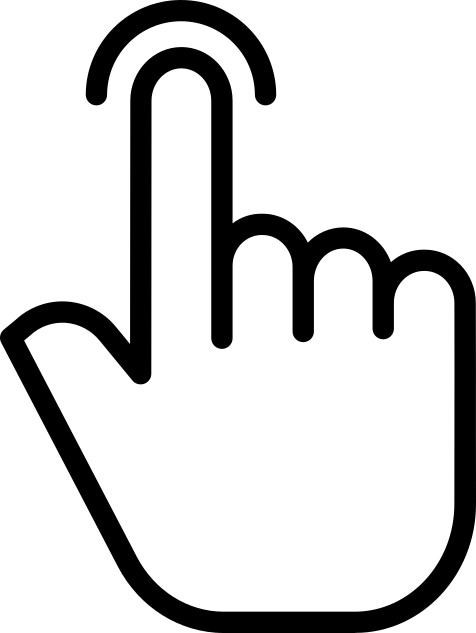
\includegraphics[width=0.10\textwidth]{static/dedo.png}} ;
    \node[const, left=of d] (nd) {\Large $s$};

    \edge {r} {d};
  }
  \caption{Modelo A: $s \neq r$}
  \label{fig:modelo_causal_1}
  \end{subfigure}
  \begin{subfigure}[b]{0.48\textwidth}
  \centering
  \tikz{

    \node[latent] (d) {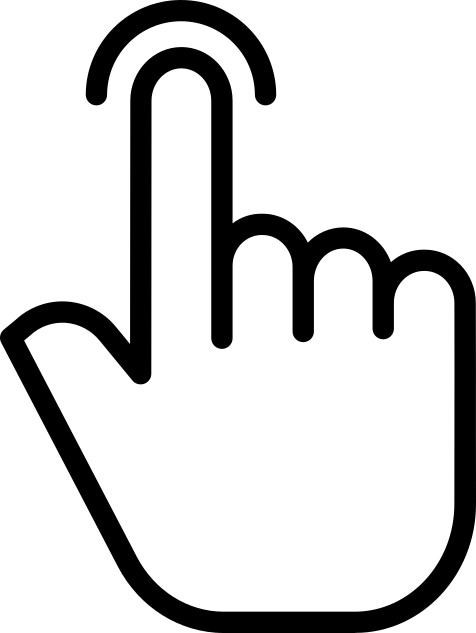
\includegraphics[width=0.10\textwidth]{static/dedo.png}} ;
    \node[const,above=of d] (nd) {\Large $s$} ;

    \node[latent, above=of d, xshift=-1.5cm] (r) {
\includegraphics[width=0.12\textwidth]{static/regalo.png}} ;
    \node[const,above=of r] (nr) {\Large $r$} ;

    \node[latent, fill=black!30, above=of d, xshift=1.5cm] (c) {
\includegraphics[width=0.12\textwidth]{static/cerradura.png}} ;
    \node[const,above=of c] (nc) {\Large $c=1$} ;

    \edge {r,c} {d};
  }
  \caption{Modelo B: $s \neq r$ y $s \neq c$}
  \label{fig:modelo_causal_2}
  \end{subfigure}
  \caption{Modelos causales alternativos. Figura~\ref{fig:modelo_causal_1}: la pista s\'olo depende de la posici\'on del regalo. Figura~\ref{fig:modelo_causal_2}: la pista depende de la posici\'on del regalo y la caja elegida previamente.
  Los c\'irculos representan las variables y la flecha representa la relaci\'on causa $\rightarrow$ efecto.
  %A su vez, $r=i$ representa la proposici\'on ``el regalo se encuentra en la posici\'on $i$'', y $s=i$ representa la proposici\'on ``la pista se\~nala la posici\'on $i$''.
  }
  \label{fig:modelos_causales}
\end{figure}

% Parrafo
% %
% Por \'ultimo, lo que aparece del lado izquierdo del operador \emph{condicional} ($\cdot \mid \cdot$) son las proposiciones sobre las que computamos la creencia en los casos en los que las proposiciones que aparecen del lado derecha sean ciertas.
% %
% Es decir, la $\text{Creencia}(s=i|r=i,\text{Modelo}) = 0$ se lee como ``es imposible que la pista se\~nale la posici\'on $i$ cuando el regalo est\'a en la posici\'on $i$ y el modelo causal es cierto''.
%

% % Parrafo

Cada uno de los modelos causales alternativos tiene su propio conjunto finito de universos paralelos.
%
Siguiendo con el principio de maximizar incertidumbre dada la información disponible, definimos la distribución de creencia honesta dividiendo la creencia en partes iguales en cada una de las bifurcaciones de los caminos paralelos del modelo causal.
%
En la figura~\ref{fig:caminos} mostramos los caminos paralelos que generan ambos modelos causales sobre los cuales se divide la creencia.

% Parrafo

En el modelo A, por cada posici\'on del regalo, se abren otros dos universos paralelos que se corresponden con las cajas hacia las que puede se\~nalar la pista, en las que no est\'a el regalo en ese universo.
%
En cambio, en el modelo B, la pista genera dos universos s\'olo cuando el regalo est\'a en la misma caja que elegimos, $r=c=1$.
%
% Podemos recibir una pista tanto en la puerta 2, $s_2$, como en la puerta 3, $s_3$.
% %
% Cuando el regalo est\'a en otra caja, $r\neq 1$, la pista puede se\~nalar \'unicamente a una de las cajas, la que no tiene el regalo y la que no fue elegida.
% %
% Por ejemplo, si el regalo est\'a en la puerta 2, $r_2$, la pista s\'olo puede se\~nalar la puerta 3, $s_3$.
%
\begin{figure}[H]
\centering
\begin{subfigure}[b]{0.48\textwidth}
\centering
\tikz{
\node[latent, draw=white, yshift=0.7cm] (b0) {$1$};

\node[latent,below=of b0,yshift=0.7cm, xshift=-2cm] (r1) {$r_1$};
\node[latent,below=of b0,yshift=0.7cm] (r2) {$r_2$};
\node[latent,below=of b0,yshift=0.7cm, xshift=2cm] (r3) {$r_3$};

\node[latent, below=of r1, draw=white, yshift=0.7cm] (br1) {$\frac{1}{3}$};
\node[latent, below=of r2, draw=white, yshift=0.7cm] (br2) {$\frac{1}{3}$};
\node[latent, below=of r3, draw=white, yshift=0.7cm] (br3) {$\frac{1}{3}$};
\node[latent,below=of br1,yshift=0.7cm, xshift=-0.5cm] (r1d2) {$s_2$};
\node[latent,below=of br1,yshift=0.7cm, xshift=0.5cm] (r1d3) {$s_3$};

\node[latent,below=of r1d2,yshift=0.7cm,draw=white] (br1d2) {$\frac{1}{3}\frac{1}{2}$};
\node[latent,below=of r1d3,yshift=0.7cm, draw=white] (br1d3) {$\frac{1}{3}\frac{1}{2}$};
\node[latent,below=of br2,yshift=0.7cm, xshift=-0.5cm] (r2d1) {$s_1$};
\node[latent,below=of br2,yshift=0.7cm, xshift=0.5cm] (r2d3) {$s_3$};
\node[latent,below=of br3,yshift=0.7cm, xshift=-0.5cm] (r3d1) {$s_1$};
\node[latent,below=of br3,yshift=0.7cm, xshift=0.5cm] (r3d2) {$s_2$};

\node[latent,below=of r2d1,yshift=0.7cm, draw=white] (br2d1) {$\frac{1}{3}\frac{1}{2}$};
\node[latent,below=of r2d3,yshift=0.7cm,draw=white] (br2d3) {$\frac{1}{3}\frac{1}{2}$};
\node[latent,below=of r3d1,yshift=0.7cm, draw=white] (br3d1) {$\frac{1}{3}\frac{1}{2}$};
\node[latent,below=of r3d2,yshift=0.7cm,draw=white] (br3d2) {$\frac{1}{3}\frac{1}{2}$};
\edge[-] {b0} {r1,r2,r3};
\edge[-] {r1} {br1};
\edge[-] {r2} {br2};
\edge[-] {r3} {br3};
\edge[-] {br1} {r1d2,r1d3};
\edge[-] {r1d2} {br1d2};
\edge[-] {r1d3} {br1d3};
\edge[-] {br2} {r2d1, r2d3};
\edge[-] {br3} {r3d1,r3d2};
\edge[-] {r2d1} {br2d1};
\edge[-] {r2d3} {br2d3};
\edge[-] {r3d1} {br3d1};
\edge[-] {r3d2} {br3d2};
}
\caption{Modelo A}
\label{fig:caminos_pre_montyhall}
\end{subfigure}
\begin{subfigure}[b]{0.48\textwidth}
\centering
\tikz{
\node[latent, draw=white, yshift=0.7cm] (b0) {$1$};
\node[latent,below=of b0,yshift=0.7cm, xshift=-2cm] (r1) {$r_1$};
\node[latent,below=of b0,yshift=0.7cm] (r2) {$r_2$};
\node[latent,below=of b0,yshift=0.7cm, xshift=2cm] (r3) {$r_3$};

% \node[latent, below=of r1, draw=white, yshift=0.8cm] (br1) {$\frac{1}{3}$};
% \node[latent, below=of r2, draw=white, yshift=0.8cm] (br2) {$\frac{1}{3}$};
% \node[latent, below=of r3, draw=white, yshift=0.8cm] (br3) {$\frac{1}{3}$};
% \node[latent,below=of br1,yshift=0.8cm] (c11) {$c_1$};
% \node[latent,below=of br2,yshift=0.8cm] (c12) {$c_1$};
% \node[latent,below=of br3,yshift=0.8cm] (c13) {$c_1$};

\node[latent, below=of r1, draw=white, yshift=0.7cm] (bc11) {$\frac{1}{3}$};
\node[latent, below=of r2, draw=white, yshift=0.7cm] (bc12) {$\frac{1}{3}$};
\node[latent, below=of r3, draw=white, yshift=0.7cm] (bc13) {$\frac{1}{3}$};
\node[latent,below=of bc11,yshift=0.7cm, xshift=-0.5cm] (r1d2) {$s_2$};
\node[latent,below=of bc11,yshift=0.7cm, xshift=0.5cm] (r1d3) {$s_3$};
\node[latent,below=of bc12,yshift=0.7cm] (r2d3) {$s_3$};
\node[latent,below=of bc13,yshift=0.7cm] (r3d2) {$s_2$};

\node[latent,below=of r1d2,yshift=0.7cm,draw=white] (br1d2) {$\frac{1}{3}\frac{1}{2}$};
\node[latent,below=of r1d3,yshift=0.7cm, draw=white] (br1d3) {$\frac{1}{3}\frac{1}{2}$};
\node[latent,below=of r2d3,yshift=0.7cm,draw=white] (br2d3) {$\frac{1}{3}$};
\node[latent,below=of r3d2,yshift=0.7cm,draw=white] (br3d2) {$\frac{1}{3}$};
\edge[-] {b0} {r1,r2,r3};
% \edge[-] {r1} {br1};
% \edge[-] {r2} {br2};
% \edge[-] {r3} {br3};
% \edge[-] {br1} {c11};
% \edge[-] {br2} {c12};
% \edge[-] {br3} {c13};
\edge[-] {r1} {bc11};
\edge[-] {r2} {bc12};
\edge[-] {r3} {bc13};
\edge[-] {bc11} {r1d2,r1d3};
\edge[-] {bc12} {r2d3};
\edge[-] {bc13} {r3d2};
\edge[-] {r1d2} {br1d2};
\edge[-] {r1d3} {br1d3};
\edge[-] {r2d3} {br2d3};
\edge[-] {r3d2} {br3d2};
}
\caption{Modelo B}
\label{fig:caminos_montyhall}
\end{subfigure}
\caption{Los caminos paralelos que se generan a partir de los modelos causales alternativos. El principio de m\'axima incertidumbre dada la información disponible divide la creencia en partes iguales en cada una de las bifurcaciones de los caminos paralelos del modelo causal.}
\label{fig:caminos}
\end{figure}
%
La creencia en las hojas de los universo paralelo del modelo causal representa la \emph{creencia conjunta} honesta de que el regalo se encuentre en la caja $i$ y la pista se\~nale la caja $j$, $P(r=i, s=j|\text{Modelo})$.
%
\begin{table}[ht!]
\centering
$P(r=i, s=j | \text{Modelo A})$ \hspace{1.8cm} $P(r=i, s=j | \text{Modelo B})$ \\[0.1cm]
 \begin{tabular}{|c|c|c|c|} \hline \setlength\tabcolsep{0.4cm}
       & \, $r_1$ \, &  \, $r_2$ \, & \, $r_3$ \, \\ \hline
  $s_1$ & $0$ & $1/6$ & $1/6$  \\ \hline
  $s_2$ & $1/6$ & $0$ & $1/6$  \\ \hline
  $s_3$ & $1/6$ & $1/6$ & $0$ \\ \hline
  \end{tabular}
  \hspace{1.5cm}
  \begin{tabular}{|c|c|c|c|} \hline  \setlength\tabcolsep{0.4cm}
 & \, $r_1$ \, &  \, $r_2$ \, & \, $r_3$ \,  \\ \hline
  $s_1$ & $0$ & $0$ & $0$ \\ \hline
  $s_2$ & $1/6$ & $0$ & $1/3$ \\ \hline
  $s_3$ & $1/6$ & $1/3$ & $0$  \\ \hline
  \end{tabular}
  \caption{Creencia conjunta honesta para cada uno de los modelos causales. Las celdas representan universos paralelos y el valor la creencia asignada a cada uno de ellos.}
  \label{tab:creencia_conjunta}
\end{table}
%
%La conjunci\'on l\'ogica la expresamos con una simple coma ($,$), y colocamos del lado derecho del condicional ($\cdot|\cdot$) las proposiciones que momentáneamente consideramos ciertas.
%
Cada una de las celdas de la tabla representa una de las terminales de los universos paralelos representados en la figura \ref{fig:caminos}.

% Parrafo

Por el ``principio de integridad'', la creencia asignada a una variable individual (creencia marginal) es la suma de todos los caminos paralelos (creencia conjunta) en los que esa variable est\'a presente.
%
\begin{equation}
\begin{split}
P(s_j|\text{Modelo A}) = \sum_i P(r_i, s_j|\text{Modelo A}) = 1/3 \\  P(s_j|\text{Modelo B}) = \sum_i P(r_i, s_j|\text{Modelo B}) = 1/2
\end{split}
\end{equation}

% Parrafo

Lo mismo ocurre con cualquiera de las variables de un modelo multidimensional.
% \begin{table}[H]
% \centering
% Modelo A  \hspace{4.5cm}  Modelo B \\[0.1cm]
%  \begin{tabular}{|c|c|c|c||c|} \hline \setlength\tabcolsep{0.4cm}
%        & \, $r_1$ \, &  \, $r_2$ \, & \, $r_3$ \, & \\ \hline
%   $s_1$ & $0$ & $1/6$ & $1/6$ & $1/3$ \\ \hline
%   $s_2$ & $1/6$ & $0$ & $1/6$ & $1/3$ \\ \hline
%   $s_3$ & $1/6$ & $1/6$ & $0$ & $1/3$ \\ \hline \hline
%    & $1/3$ & $1/3$ & $1/3$ & $1$ \\ \hline
%   \end{tabular}
%   \hspace{1.5cm}
%   \begin{tabular}{|c|c|c|c||c|} \hline  \setlength\tabcolsep{0.4cm}
%  & \, $r_1$ \, &  \, $r_2$ \, & \, $r_3$ \, & \\ \hline
%   $s_1$ & $0$ & $0$ & $0$ & $0$\\ \hline
%   $s_2$ & $1/6$ & $0$ & $1/3$ & $1/2$ \\ \hline
%   $s_3$ & $1/6$ & $1/3$ & $0$ & $1/2$ \\ \hline \hline
%    & $1/3$ & $1/3$ & $1/3$ & $1$  \\ \hline
%   \end{tabular}
%   \caption{Creencia marginal honesta obtenida mediante el principio de integridad, como la suma de la creencia asignada a todos los universos en los que esa variable est\'a presente.}
%   \label{tab:creencia_marginal}
% \end{table}
En ambos modelos la creencia marginal honesta sobre el regalos es $1/3$
%
\begin{figure}[H]
\centering
\tikz{ %
         \node[factor, minimum size=1cm] (p1) {
\includegraphics[width=0.025\textwidth]{static/cerradura.png}} ;
         \node[factor, minimum size=1cm, xshift=1.5cm] (p2) {} ;
         \node[factor, minimum size=1cm, xshift=3cm] (p3) {} ;

         \node[const, above=of p1, yshift=.15cm] (fp1) {$1/3$};
         \node[const, above=of p2, yshift=.15cm] (fp2) {$1/3$};
         \node[const, above=of p3, yshift=.15cm] (fp3) {$1/3$};
         \node[const, below=of p2, yshift=-.10cm, xshift=0.3cm] (dedo) {};
        }
\caption{Creencia marginal honesta sobre el regalo en ambos modelos causales. }
\end{figure}

\subsection{Principio de coherencia} \label{sec:principio_choerencia} % (dados los datos de base emp\'irica)

El principio de no mentir nos permiti\'o definir la creencia conjunta honesta inicial, y el principio de integridad nos permiti\'o derivar de ella la creencia marginal honesta.
%
¿Pero c\'omo para preservar los acuerdos intersubjetivos cuando recibimos nueva informaci\'on?
%
El principio de coherencia establece que la nueva creencia honesta, despu\'es de haber visto un nuevo dato, es la creencia previa que sigue siendo compatible con ese dato.

% Parrafo

Supongamos que alguien nos indica con certeza que el regalo no est\'a en la caja del medio.
%
¿Cu\'al es la nueva creencia marginal honesta sobre el regalo despu\'es de haber visto esta pista?

% Parrafo

\begin{figure}[ht!]
\centering
\tikz{ %

         \node[factor, minimum size=1cm] (p1) {
\includegraphics[width=0.025\textwidth]{static/cerradura.png}} ;
         \node[det, minimum size=1cm, xshift=1.5cm] (p2) {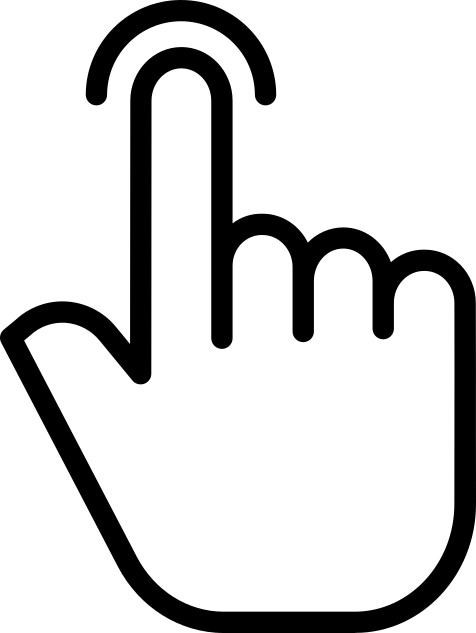
\includegraphics[width=0.03\textwidth]{static/dedo.png}} ;
         \node[factor, minimum size=1cm, xshift=3cm] (p3) {} ;
         \node[const, above=of p1, yshift=.15cm] (fp1) {$?$};
         \node[const, above=of p2, yshift=.15cm] (fp2) {$?$};
         \node[const, above=of p3, yshift=.15cm] (fp3) {$?$};
         \node[const, below=of p2, yshift=-.10cm, xshift=0.3cm] (dedo) {};

        }
\end{figure}

% Parrafo
%
% Para actualizar las creencias posiblemente nos veamos tentados a aplicar el principio de indiferencia nuevamente, asignando $0.5$ a las dos cajas restantes.
% %
% Aunque esa propuesta coincida con la soluci\'on correcta que obtendremos para el modelo A, esa
% decisi\'on conduce a errores en t\'erminos generales.
% %
% El principio de indiferencia s\'olo se aplica una \'unica vez, al inicio.
% %
% Despu\'es s\'olo actualizaremos esa creencia en funci\'on de la nueva informaci\'on que vayamos incorporando.
%
% % Parrafo

Para actualizar las creencias simplemente nos quedamos con la creencia previa que es compatible con el dato.
%
Para ello nos quedamos con los caminos paralelos del modelo causal que siguen siendo compatible con el observable, $P(r_i, s_2)$.
%
\begin{table}[ht!]
\centering
$P(r=i, s=2 | \text{Modelo A})$ \hspace{2.7cm} $P(r=i, s=2 | \text{Modelo B})$ \\[0.1cm]
\begin{tabular}{|c|c|c|c||c|} \hline \setlength\tabcolsep{0.4cm}
       & \, $r_1$ \, &  \, $r_2$ \, & \, $r_3$ \, & \\ \hline
  $s_2$ & $1/6$ & $0$ & $1/6$ & $1/3$ \\ \hline
  \end{tabular}
  \hspace{1.5cm}
  \begin{tabular}{|c|c|c|c||c|} \hline  \setlength\tabcolsep{0.4cm}
 & \, $r_1$ \, &  \, $r_2$ \, & \, $r_3$ \, & \\ \hline
  $s_2$ & $1/6$ & $0$ & $1/3$ & $1/2$ \\ \hline
  \end{tabular}
  \caption{La creencia conjunta y marginal que sobrevive luego de ver el dato.}
  \label{tab:creencia_compatible}
\end{table}

En la tabla~\ref{tab:creencia_compatible} nos quedamos con la creencia conjunta y marginal que sigue siendo compatible con el dato.
%
Esto es exactamente lo mismo que quedarnos con los caminos del modelo causal que son posibles dado el modelo causal y el observable.
%
En la figura~\ref{fig:caminos_compatibles} mostramos los caminos que son compatibles en negro y los incompatibles en gris.

\begin{figure}[ht!]
\centering
\begin{subfigure}[b]{0.48\textwidth}
\centering
\tikz{
\node[latent, draw=white, yshift=0.7cm] (b0) {$1$};

\node[latent,below=of b0,yshift=0.7cm, xshift=-2cm] (r1) {$r_1$};
{\color{gray}\node[latent,draw=gray,below=of b0,yshift=0.7cm] (r2) {$r_2$};}
\node[latent,below=of b0,yshift=0.7cm, xshift=2cm] (r3) {$r_3$};

\node[latent, below=of r1, draw=white, yshift=0.7cm] (br1) {$\frac{1}{3}$};
{\color{gray}\node[latent, below=of r2, draw=white, yshift=0.7cm] (br2) {$\frac{1}{3}$};}
\node[latent, below=of r3, draw=white, yshift=0.7cm] (br3) {$\frac{1}{3}$};
\node[latent,below=of br1,yshift=0.7cm, xshift=-0.5cm] (r1d2) {$s_2$};
{\color{gray}\node[latent,draw=gray,below=of br1,yshift=0.7cm, xshift=0.5cm] (r1d3) {$s_3$};}

\node[latent,below=of r1d2,yshift=0.7cm,draw=white] (br1d2) {$\frac{1}{3}\frac{1}{2}$};
{\color{gray} \node[latent,draw=gray,below=of r1d3,yshift=0.7cm, draw=white] (br1d3) {$\frac{1}{3}\frac{1}{2}$}; }
{\color{gray}\node[latent,draw=gray,below=of br2,yshift=0.7cm, xshift=-0.5cm] (r2d1) {$s_1$}; }
{\color{gray} \node[latent,draw=gray,below=of br2,yshift=0.7cm, xshift=0.5cm] (r2d3) {$s_3$}; }
{\color{gray} \node[latent,draw=gray,below=of br3,yshift=0.7cm, xshift=-0.5cm] (r3d1) {$s_1$}; }
\node[latent,below=of br3,yshift=0.7cm, xshift=0.5cm] (r3d2) {$s_2$};

{\color{gray}\node[latent,below=of r2d1,yshift=0.7cm, draw=white] (br2d1) {$\frac{1}{3}\frac{1}{2}$};}
{\color{gray}\node[latent,below=of r2d3,yshift=0.7cm,draw=white] (br2d3) {$\frac{1}{3}\frac{1}{2}$};}
{\color{gray}\node[latent,below=of r3d1,yshift=0.7cm, draw=white] (br3d1) {$\frac{1}{3}\frac{1}{2}$};}
\node[latent,below=of r3d2,yshift=0.7cm,draw=white] (br3d2) {$\frac{1}{3}\frac{1}{2}$};
\edge[-] {b0} {r1,r3};
\edge[-,draw=gray] {b0} {r2};
\edge[-] {r1} {br1};
\edge[-,draw=gray] {r2} {br2};
\edge[-] {r3} {br3};
\edge[-] {br1} {r1d2};
\edge[-,draw=gray] {br1} {r1d3};
\edge[-] {r1d2} {br1d2};
\edge[-,draw=gray] {r1d3} {br1d3};
\edge[-, draw=gray] {br2} {r2d1, r2d3};
\edge[-] {br3} {r3d2};
\edge[-, draw=gray] {br3} {r3d1};
\edge[-, draw=gray] {r2d1} {br2d1};
\edge[-, draw=gray] {r2d3} {br2d3};
\edge[-, draw=gray] {r3d1} {br3d1};
\edge[-] {r3d2} {br3d2};
}
\caption{Modelo A}
\label{fig:caminos_pre_montyhall_compatibles}
\end{subfigure}
\begin{subfigure}[b]{0.48\textwidth}
\centering
\tikz{
\node[latent, draw=white, yshift=0.7cm] (b0) {$1$};
\node[latent,below=of b0,yshift=0.7cm, xshift=-2cm] (r1) {$r_1$};
{\color{gray}\node[latent,draw=gray,below=of b0,yshift=0.7cm] (r2) {$r_2$}; }
\node[latent,below=of b0,yshift=0.7cm, xshift=2cm] (r3) {$r_3$};

% \node[latent, below=of r1, draw=white, yshift=0.8cm] (br1) {$\frac{1}{3}$};
% \node[latent, below=of r2, draw=white, yshift=0.8cm] (br2) {$\frac{1}{3}$};
% \node[latent, below=of r3, draw=white, yshift=0.8cm] (br3) {$\frac{1}{3}$};
% \node[latent,below=of br1,yshift=0.8cm] (c11) {$c_1$};
% \node[latent,below=of br2,yshift=0.8cm] (c12) {$c_1$};
% \node[latent,below=of br3,yshift=0.8cm] (c13) {$c_1$};

\node[latent, below=of r1, draw=white, yshift=0.7cm] (bc11) {$\frac{1}{3}$};
{\color{gray}\node[latent, below=of r2, draw=white, yshift=0.7cm] (bc12) {$\frac{1}{3}$};}
\node[latent, below=of r3, draw=white, yshift=0.7cm] (bc13) {$\frac{1}{3}$};
\node[latent,below=of bc11,yshift=0.7cm, xshift=-0.5cm] (r1d2) {$s_2$};
{\color{gray}\node[latent,draw=gray,below=of bc11,yshift=0.7cm, xshift=0.5cm] (r1d3) {$s_3$};}
{\color{gray}\node[latent, draw=gray,below=of bc12,yshift=0.7cm] (r2d3) {$s_3$};}
\node[latent,below=of bc13,yshift=0.7cm] (r3d2) {$s_2$};

\node[latent,below=of r1d2,yshift=0.7cm,draw=white] (br1d2) {$\frac{1}{3}\frac{1}{2}$};
{\color{gray}\node[latent,below=of r1d3,yshift=0.7cm, draw=white] (br1d3) {$\frac{1}{3}\frac{1}{2}$};}
{\color{gray}\node[latent,below=of r2d3,yshift=0.7cm,draw=white] (br2d3) {$\frac{1}{3}$};}
\node[latent,below=of r3d2,yshift=0.7cm,draw=white] (br3d2) {$\frac{1}{3}$};
\edge[-] {b0} {r1,r3};
\edge[-,draw=gray] {b0} {r2};
% \edge[-] {r1} {br1};
% \edge[-] {r2} {br2};
% \edge[-] {r3} {br3};
% \edge[-] {br1} {c11};
% \edge[-] {br2} {c12};
% \edge[-] {br3} {c13};
\edge[-] {r1} {bc11};
\edge[-,draw=gray] {r2} {bc12};
\edge[-] {r3} {bc13};
\edge[-] {bc11} {r1d2};
\edge[-,draw=gray] {bc11} {r1d3};
\edge[-,draw=gray] {bc12} {r2d3};
\edge[-] {bc13} {r3d2};
\edge[-] {r1d2} {br1d2};
\edge[-,draw=gray] {r1d3} {br1d3};
\edge[-,draw=gray] {r2d3} {br2d3};
\edge[-] {r3d2} {br3d2};
}
\caption{Modelo B}
\label{fig:caminos_montyhall_compatibles}
\end{subfigure}
\caption{Los caminos paralelos compatibles (negro) e incompatibles (gris) con el dato $s=2$. }
\label{fig:caminos_compatibles}
\end{figure}
% Cuando aplicamos por primera vez el principio de indiferencia en la figura \ref{fig:principio_de_indiferencia}, el espacio de hip\'otesis se reduc\'ia a tres opciones, una por caja.
% %
% En este caso, en el que estamos considerando una variable nueva (la se\~nal $s$) que representa la pista, el espacio de hip\'otesis es otro, m\'as grande, por lo que esta creencia a priori no nos sirve.
% %

Es decir, para actualizar nuestra creencia nos quedamos con la creencia a priori que es compatible con los datos.
%
Lo que nos permitir\'a cumplir el objetivo que nos hab\'iamos propuesto, actualizar la creencia sobre el regalo luego de haber visto la pista.
%
\textbf{La creencia que sobrevive}, $P(r_i, s_2)$, es ahora nuestra nueva creencia total.
%
Para expresarla nuevamente como tal, la normalizamos para que vuelva a sumar 1.
%
\begin{equation}
P(r_i| s_2, \text{Modelo} ) = \frac{P(r_i, s_2| \text{Modelo})}{P(s_2| \text{Modelo})}
\end{equation}
%
La concusi\'on a la que llegamos depende del modelo causal elegido.
\begin{figure}[ht!]
\centering
\begin{subfigure}[b]{0.48\textwidth}
\centering
\tikz{ %

         \node[factor, minimum size=1cm] (p1) {
\includegraphics[width=0.05\textwidth]{static/cerradura.png}} ;
         \node[det, minimum size=1cm, xshift=1.5cm] (p2) {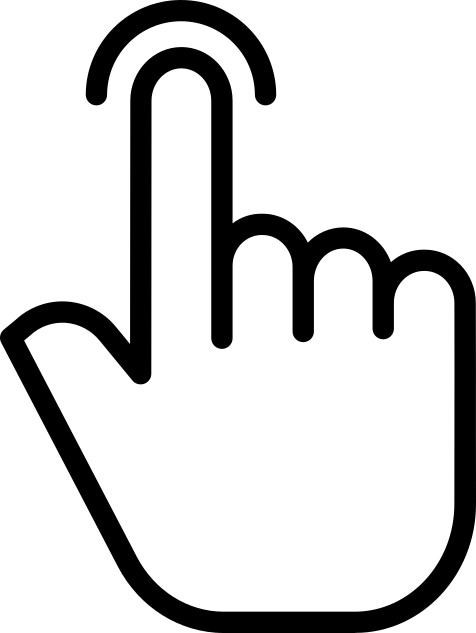
\includegraphics[width=0.06\textwidth]{static/dedo.png}} ;
         \node[factor, minimum size=1cm, xshift=3cm] (p3) {} ;

         \node[const, above=of p1, yshift=.15cm] (fp1) {$1/2$};
         \node[const, above=of p2, yshift=.15cm] (fp2) {$0$};
         \node[const, above=of p3, yshift=.15cm] (fp3) {$1/2$};
         \node[const, below=of p2, yshift=-.10cm, xshift=0.3cm] (dedo) {};
}
\caption{Modelos A}
\end{subfigure}
\begin{subfigure}[b]{0.48\textwidth}
\centering
\tikz{ %

         \node[factor, minimum size=1cm] (p1) {
\includegraphics[width=0.05\textwidth]{static/cerradura.png}} ;
         \node[det, minimum size=1cm, xshift=1.5cm] (p2) {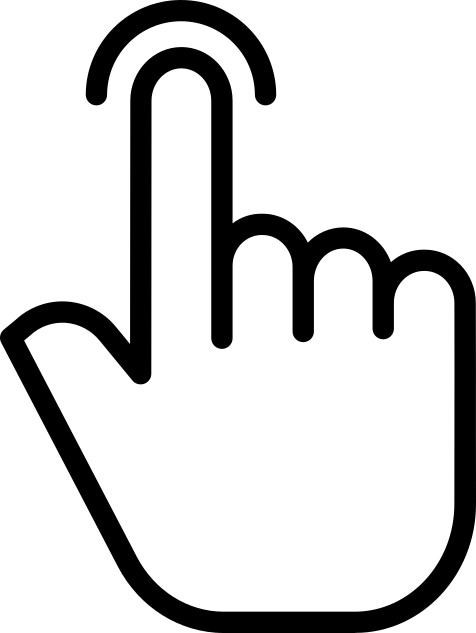
\includegraphics[width=0.06\textwidth]{static/dedo.png}} ;
         \node[factor, minimum size=1cm, xshift=3cm] (p3) {} ;

         \node[const, above=of p1, yshift=.15cm] (fp1) {$1/3$};
         \node[const, above=of p2, yshift=.15cm] (fp2) {$0$};
         \node[const, above=of p3, yshift=.15cm] (fp3) {$2/3$};
         \node[const, below=of p2, yshift=-.10cm, xshift=0.3cm] (dedo) {};
        }
\caption{Modelo B}
\end{subfigure}
\caption{Nueva creencia honesta dada el dato y el modelo}
\end{figure}
%
Si bien ambas respuesta son diferentes, ambas comparten la propiedad de ser la distribuci\'on de creencias que maximiza la incertidumbre dada la evidencia formal (modelo causal) y emp\'irica (datos), el acuerdo intersubjetivo si el modelo causal y los datos fueran ciertos.

\section{Las reglas de la probabilidad}\label{sec:reglas_de_la_probabilidad}

La teor\'ia de la probabilidad es actualmente el enfoque más utilizado para representar incertidumbre asociada al conocimiento emp\'irico.
%
La teor\'ia de la probabilidad puede resumirse en dos reglas, conocidas como la regla de la suma y la regla del producto.
%
La regla de la suma proviene del principio de integridad y establece que cualquier creencia marginal puede ser obtenida integrando la creencia conjunta.
%
\begin{equation}
P(r_i) = \sum_j P(r_i, s_j)
\end{equation}
%
La segunda regla proviene del principio de coherencia y, expresada como producto, establece que cualquier distribuci\'on conjunta puede ser expresada como el producto de distribuciones condicionales uni-dimensionales.
%
\begin{equation}
P(s_j)P(r_i|s_j) = P(r_i, s_j)
\end{equation}

% Parrafo

Las reglas de la probabilidad han sido derivadas formalmente a partir de varios sistemas axiom\'aticos conceptualmente distintos e independientes entre si, lo cual es uno de los puntos fuertes a su favor~\cite{halpern2017}.
%
El sistema axiom\'atico de Cox~\cite{cox} las deriva a partir de axiomas del ``sentido común''.
%
El sistema axiom\'atico de Ramsey~\cite{ramsey} las deriva haciendo una analog\'ia con los pagos que aceptar\'iamos en una apuesta.
%
El sistema axiom\'atico de Kolmogorov~\cite{kolmogorov} la regla de la suma forma parte de los axiomas y la regla del producto de una definici\'on complementaria.
%
Este sistema axiomático es el más utilizado y en su versión original dice,
\begin{quotation}
Sea $E$ un conjunto de elementos y $F$ un conjunto de subconjuntos de $E$.
%
\begin{enumerate}\itemsep-0.05cm
\item $F$ est\'a cerrada bajo complementos, uniones e intersecciones contables.
\item $F$ contiene al conjunto $E$
\item Todo conjunto $S \in F$ se le asigna una n\'umero real no negativo, $P(S)$.
\item $P(E) = 1$
\item Si $S_1, S_2, \dots$ son conjuntos mutuamente excluyente, luego
\begin{equation}
P(S_1 \cup S_2 \cup \dots ) = \sum P(S_i)
\end{equation}
\end{enumerate}
\end{quotation}
%
% La regla de la suma se deriva inmediatamente del axioma 5 dado que siempre podemos expresar cualquier conjunto como $A = A \cap (B \cup \neg B)$.
% %
La probabilidad condicional (o regla del producto) se incluye en el sistema como una definici\'on que cumple con los axiomas de la probabilidad.

% %Ciertamentese ha dedicado mucho m\'as esfuerzo a justificar la teor\'ia de la probabilidad que cualquier otro enfoque para representar la incertidumbre y el tiempo dir\'a si se pueden se pueden desarrollar otros enfoques superadores.
% Pero quiz\'as m\'as importante es que su aplicaci\'on estricta (lo que llamamos inferencia Bayesiana) garantiza los acuerdos intersubjetivos a trav\'es de la maximizaci\'on de la incertidumbre (entrop\'ia) dada la informaci\'on emp\'irica y formal (datos y modelos causales)~\cite{Jaynes2003}.
% %

% Parrafo

% As\'i expresada, la teor\'ia de la probabilidad est\'a basada en s\'olo dos de los cuatro principios vistos anteriormente, y carece de criterio para definir distribuciones de creencias iniciales (inferencia Bayesiana) y para expresar relaciones causales (inferencia causal).

\subsection{Teorema de Bayes}

El teorema de Bayes no es m\'as que un corolario de las reglas de las probabilidad, que surge de aplicar dos veces la regla del producto.
%
Usando las variables vistas en la secci\'on anterior, el teorema de Bayes puede expresarse como,
%
\begin{equation}
\begin{split}
P(r_i|s_2) = \frac{P(r_i, s_2)}{P(s_2)} = \frac{P(s_2|r_i)P(r_i)}{P(s_2)}
\end{split}
\end{equation}
%
Es una pr\'actica muy com\'un dejar impl\'icita la dependencia respecto del modelo causal.
%
Lo correcto ser\'ia incluirlo en el condicional.
%
Notar adem\'as que escribimos a $r$ con un sub\'indice $i$ y a $s$ con un sub\'indice $2$.
%
Con esto queremos connotar la idea de que $r_i$ es una variable libre, que queremos evaluar para los diferentes valores (la hip\'otesis), y $s_2$ es un valor constante (el dato observado).
%
En l\'inea con esta interpretaci\'on, volvemos a expresar el teorema de Bayes de la siguiente manera.
% %
% \begin{equation*}
% \underbrace{P(\text{Hip\'otesis }|\text{ Datos})}_{\text{\scriptsize Posteriori}} = \frac{\overbrace{P(\text{Datos }|\text{ Hip\'otesis})}^{\text{\scriptsize Verosimilitud}} \overbrace{P(\text{Hip\'otesis})}^{\text{\scriptsize Priori}} }{\underbrace{P(\text{Datos})}_{\text{\scriptsize Evidencia}}}
% \end{equation*}
%
\begin{equation*}
\underbrace{P(\text{Hip\'otesis }|\text{ Datos, Modelo})}_{\text{\scriptsize Posterior}} = \frac{\overbrace{P(\text{Datos }|\text{ Hip\'otesis, Modelo})}^{\text{\scriptsize Verosimilitud}} \overbrace{P(\text{Hip\'otesis }|\text{ Modelo})}^{\text{\scriptsize Prior}} }{\underbrace{P(\text{Datos }|\text{ Modelo})}_{\text{\scriptsize Evidencia}}}
\end{equation*}
%
Los diferentes factores del teorema de Bayes han recibido nombres a lo largo de la historia, que revisemos a continuaci\'on.

\subsection{Prior}

El \emph{prior} es la distribuci\'on de creencia inicial de las hip\'otesis dado el modelo causal antes de ver los datos.
%
En la secci\'on \emph{\nameref{sec:principio_indiferencia}} hemos visto un criterio intercultural que nos permite alcanzar un primer acuerdo intersubjetivo en contextos de incertidumbre.
%
El enfoque ``frecuentista'' de la teor\'ia de la probabilidad, al rechazar todo criterio para definir distribuciones de creencias iniciales, se ve impedido de utilizar el teorema de Bayes.
%
Como consecuencia, en vez de ofrecer distribuciones de probabilidad sobre todo el espacio de hip\'otesis, este enfoque suele seleccionar una \'unica hip\'otesis (estimaci\'on puntual) en base a funciones de costo ad-hoc, siendo las m\'as com\'un la maximizaci\'on de la verosimilitud.

\subsection{Verosimilitud}

La \emph{verosimilitud} es la predicci\'on del dato observado cuando suponemos que la hip\'otesis que estamos evaluando es cierta.
%
Veamos cu\'al es la verosimilitud, $P(s2|r_i, \text{Modelo B})$, la probabilidad de que la pista haya se\~nalado la caja $2$ en el modelo de Monty Hall para las diferentes posibles posiciones del regalo $r_i$.
%
\begin{figure}[ht!]
\begin{subfigure}[b]{0.7\textwidth}
\centering
\tikz{
\phantom{\node[latent, draw=white, yshift=0.8cm] (b0) {$1$};}
\node[latent,below=of b0,yshift=0.8cm, xshift=-2.5cm] (r1) {$r_1$};
\node[latent,below=of b0,yshift=0.8cm] (r2) {$r_2$};
\node[latent,below=of b0,yshift=0.8cm, xshift=1.8cm] (r3) {$r_3$};

\node[latent, below=of r1, draw=white, yshift=0.8cm] (br1) {$1$};
\node[latent, below=of r2, draw=white, yshift=0.8cm] (br2) {$1$};
\node[latent, below=of r3, draw=white, yshift=0.8cm] (br3) {$1$};

\node[latent,below=of br1,yshift=0.8cm, xshift=-0.7cm] (r1d2) {$s_2$};
\node[latent,below=of br1,yshift=0.8cm, xshift=0.7cm] (r1d3) {$s_3$};
\node[latent,below=of br2,yshift=0.8cm] (r2d3) {$s_3$};
\node[latent,below=of br3,yshift=0.8cm] (r3d2) {$s_2$};

\node[latent,below=of r1d2,yshift=0.8cm,draw=white] (br1d2) {$\frac{1}{2}$};
\node[latent,below=of r1d3,yshift=0.8cm, draw=white] (br1d3) {$\frac{1}{2}$};
\node[latent,below=of r2d3,yshift=0.8cm,draw=white] (br2d3) {$1$};
\node[latent,below=of r3d2,yshift=0.8cm,draw=white] (br3d2) {$1$};
\phantom{\edge[-] {b0} {r1,r2,r3};}
\edge[-] {r1} {br1};
\edge[-] {r2} {br2};
\edge[-] {r3} {br3};
\edge[-] {br1} {r1d2,r1d3};
\edge[-] {br2} {r2d3};
\edge[-] {br3} {r3d2};
\edge[-] {r1d2} {br1d2};
\edge[-] {r1d3} {br1d3};
\edge[-] {r2d3} {br2d3};
\edge[-] {r3d2} {br3d2};
}
\caption{Modelos causales B cuando conocemos la posici\'on del regalo.}
\end{subfigure}
\begin{subfigure}[b]{0.29\textwidth}
\centering
 $P(s_2|r_i,\text{Modelo B})$

 \begin{tabular}{c|c|c|c} \setlength\tabcolsep{0.4cm}
          & \, $r_1$ \, &  \, $r_2$ \, & \, $r_3$ \, \\ \hline
   $s_2$ & $1/2$ & $0$ & $1$  \\ \hline
\end{tabular}
\vspace{1cm}
\caption{Verosimilitud}
\end{subfigure}
\caption{Predicci\'on del dato observado dado que el modelo causal B y la hip\'otesis son ciertas. }
\end{figure}

% Parrafo

Cuando el regalo est\'a en la misma posici\'on que la caja elegida $r=c=1$, el modelo causal permite que la pista se\~nale cualquiera de la otras dos cajas, por lo que la creencia a priori de que la caja se\~nalada sea la $s=2$ es $1/2$.
%
Cuando el regalo est\'a en una caja distinta a la elegida $r\neq c$, el modelo causal limita la pista a una \'unica caja.
%
Si el regalo est\'a en la caja $r=2$, la creencia a priori de que la caja se\~nalada sea la $s=2$ es $0$.
%
Y si el regalo est\'a en la caja $r=3$, la creencia a priori de que la caja se\~nalada sea la $s=2$ es $1$.

\subsection{Posterior}

En la secci\'on \emph{\nameref{sec:principio_choerencia}} vimos que la nueva creencia no es m\'as que la creencia previa que sigue siendo compatible con el dato.
%
El teorema de Bayes nos permite ahora reconocer que la sorpresa que produce el dato observado es lo que act\'ua como filtro de las creencias previas.
%
Debido a que el denominador del teorema de Bayes es constante, la distribuci\'on de creencias a posteriori es proporcional al producto entre el prior y la verosimilitud.
%
\begin{table}[ht!]
\centering

$P(r_i|s_2, \text{M}_B) \propto P(r_i| \text{M}_B) P(s_2|r_i, \text{M}_B) $ \\[0.2cm]

\begin{tabular}{l|c|c|c} \setlength\tabcolsep{0.4cm}
          & \, $r_1$ \, &  \, $r_2$ \, & \, $r_3$ \, \\ \hline
   $P(s_2|r_i,\text{M}_B)$ & $1/2$ & $0$ & $1$  \\ \hline
   $P(r_i,\text{M}_B)$ & $1/3$ & $1/3$ & $1/3$  \\ \hline
   $P(r_i|s_2,\text{M}_B) \propto$ & $1/6$ & $0$ & $1/3$\\ \hline
\end{tabular}
\end{table}

% Parrafo

Como las verosimilitudes son predicciones, sus valores van entre $0$ y $1$.
%
Si la hip\'otesis $r=2$ fuera cierta, la sorpresa producida cuando observamos que la pista se\~nala la caja $s=2$ ser\'ia total.
%
En ese caso, como la predicci\'on del dato observado es $0$, nada del la creencia priori sobre $r=2$ pasa a la creencia a posteriori.
%
So la hip\'otesis $r=3$ fuera cierta, la sorpresa producida cuando observamos que la pista se\~nala la caja $s=2$ es nula.
%
En ese caso, como la predicci\'on del dato observado es $1$, toda la creencia priori sobre $r=2$ pasa a la creencia a posteriori.

% Parrafo

En inferencia Bayesiana entonces, el complemento de la verosimilitud (la sorpresa) funciona como el filtro de las creencias previas.

\subsection{Evidencia}

De forma similar a la verosimilitud, la evidencia es una predicci\'on a priori del dato observado, pero que est\'a hecha con la contribuci\'on de todas las hip\'otesis.
%
Por la reglas de la probabilidad, el denominador del teorema de Bayes puede expresarse como una suma sobre todos los posibles valores del numerador, uno por cada hip\'otesis.
%
Esto hace que la evidencia sea constante para las diferentes hip\'otesis, por lo que puede ser ignorado cuando se comparan hip\'otesis alternativas.
%
Sin embargo, la evidencia va a ser distinta para los diferentes modelos.
%
En el modelo B la predicci\'on a priori de que la caja se\~nalada sea $s=2$, integrando todas las hip\'otesis, es $1/2$.
%
\begin{equation}
P(s_2|M_B) = \sum_i P(s_2|r_i, M_B) P(r_i, M_B) = \frac{1}{2} \frac{1}{3} + 0 \frac{1}{3} + \frac{1}{1} \frac{1}{3} = 1/2
\end{equation}
%
Mientras que en el modelo A la predicci\'on a priori de que la caja se\~nalada sea $s=2$, integrando todas las hip\'otesis, es $1/3$.
%
\begin{equation}
P(s_2|M_A) = \sum_i P(s_2,r_i| M_A) = 1/3
\end{equation}
%
Lo que ya hab\'ia sido calculado previamente en las marginales de la tabla \ref{tab:creencia_marginal}.

% Parrafo

La evidencia ser\'a de inter\'es cuando queramos evaluar modelos causales alternativos (ver secci\'on \ref{sec:modelos_alternativos}).

%
% \subsection{Las interpretaciones de la contradicci\'on en la teor\'ia probabilidad}
% %
% % \subsection{La escuela naturalista (frecuentista)}
% %
% % \subsection{La escuela epist\'emica (Bayesiana)}
%
% Incluso las ciencias matem\'aticas, en contacto con problemas emp\'iricos, produjo diversas escuelas de pensamiento a pesar de estar regidas supuestamente bajo las mismas reglas te\'oricas.
% %
% La justificaci\'on axiom\'atica de la teor\'ia de la probabilidad no ha sido suficiente para unificar su interpretaci\'on.
% %
% El debate filos\'ofico de fondo respecto de las interpretaciones de la probabilidad tiene que ver con la soluci\'on que las dos principales escuelas le dieron al problema de la contradicci\'on: la soluci\'on epist\'emica (bayesiana) y la ontol\'ogica (frecuentista).
%
% % Parrafo
%
% En el siglo 18 el concepto de probabilidad comenz\'o a usarse en Europa para expresar creencias contradictorias en contextos de incertidumbre.
% %
% Por ejemplo, Laplace, qui\'en ten\'ia la convicci\'on de que el mundo era determinista, no pod\'ia m\'as que utilizar la probabilidad para expresar grados de creencia a hip\'otesis mutuamente contradictorias.
% %
% La estructura funcional de un mundo determinista impide por definici\'on que A y no A ocurran dadas exactamente las mismas condiciones iniciales del mundo.
% %
% M\'as all\'a de la creencia particular de Laplace, bajo este marco la contradicci\'on de creer simultanemente en A y no A es s\'olo una expresi\'on de nuestra incertidumbre, y nada dice de la naturaleza (u ontolog\'ia) del mundo.
%
% % Parrafo
%
% La soluci\'on epist\'emica, que propon\'ia creer simultaneamente en hip\'otesis mutuamente contradictorias, fue el motivo por el cual la corriente bayesiana de la teor\'ia de la probabilidad fue tan combatida a finales del siglo 19 y durante casi todo el siglo 20.
% %
% A diferencia de las tradiciones filos\'oficas de origen oriental y americano, que ya admit\'ian alg\'un tipo de contradicci\'on en su sistema de creencias, la tradici\'on filos\'ofica Europea la rechazaba por completo.
%
% % Parrafo
%
% La escuela frecuentista, tal como se ense\~na en la materia probabilidad y estad\'isitica de la facultad de ciencias exactas y naturales, define a la probabilidad como el n\'umero al que tiende una frecuencia obtenida luego de realizar varios ``experimentos independientes'' bajo ``las mismas condiciones''.
% %
% Seg\'un esta corriente la probabilidad de eventos deterministas, por ejemplo de que exista un planeta no detectado en el sistema solar, es 0 o 1 aunque no conozcamos su valor.
% %
% S\'olo los objetos no deterministas, que llaman ``variables aleatorias'', pueden adquirir valores intermedios que representan la frecuencia en la que los diferentes estado del universo se producen a partir de exactamente las mismas condiciones inciales.
% %
% De esta forma, la contradicci\'on se propone como una propiedad externa al sistema l\'ogico, propia de la naturaleza del mundo.
% %
% La escuela frecuentista, para evitar la contradicci\'on en sus sistema l\'ogico, se ve obligada a afirmar la naturaleza aleatoria del mundo, lo que representa una la soluci\'on ont\'ol\'ogica de la contracci\'on.

% \subsection{La propiedad epistémica}
%
% % Lo que veremos en esta secci\'on es que la natrualeza multiplicativa de los procesos de selecci\'on evolutiva y probabilistica tiene una serie de propiedades que garantizan la adquisici\'on de conocimiento emp\'irico.
% %
% % % Parrafo
% Todas las axiomatizaciones alternativas de la teor\'ia de la probabilidad llegan a la conclusi\'on de que la forma natural de evaluar las hip\'otesis es a trav\'es de un proceso multiplicativo, la ``regla del producto''.
% %
% Por el teorema de Bayes, la probabilidad de una hip\'otesis $h$ dado un conjunto de observables $\{d_1, \dots, d_n \}$ y un modelo causal $M$ es,
% %
% \begin{equation}
% P(h|d_1, \dots, d_n, M) = \frac{P(d_1, \dots, d_n|h, M) P(h|M)}{P(d_1, \dots, d_n| M)} \propto \overbrace{P(d_1, \dots, d_n|h, M)}^{\text{Verosimilitud conjunta}} \overbrace{P(h|M)}^{\text{Prior}}
% \end{equation}
% %
% La proporcionalidad vale debido a que el denominador es constante para las diferentes hip\'otesis.
% %
% Además, por la regla del producto la verosimilitud conjunta puede ser expresada como el producto de las predicciones a priori.
% %
% Luego, la probabilidad de una hip\'otesis a posteriori es proporcional a la probabilidad a priori multiplicada por las predicciones a priori de los datos observados.
% %
% \begin{equation}
% P(h|d_1, \dots, d_n, M) \propto P(h|M) \overbrace{P(d_1|h,M) P(d_2|h,M,d_1) \dots }^{\text{Predicciones a priori}}
% \end{equation}
% %
% A diferencia de otras funciones de costo ad-hoc, los procesos multiplicativos garantizan que la hip\'otesis que apuestan (predicen a priori) en la misma proporci\'on que la frecuencia t\'ipica, se quedar\'a a largo plazo con todos los recursos.
% %
% Por ello, los procesos multiplicativos actúan como la funci\'on de costo epistémica universal.
%
% % Parrafo
%
% Para ejemplificar, veamos lo que ocurre en un juego de apuestas, en el que una casa de apuestas ofrece pagos $Q_c$ y $Q_s$ por Cara y Seca sobre una moneda con frecuencia $p$ e individualmente nos vemos obligados a apostar todos los recursos asignando una propoci\'on $b$ a Caras y el resto a Seca $(1-b)$.
% %
% No es dif\'icil demostrar que la soluci\'on \'optima en ambas es equivalente.
% %
% Por ello, de aqu\'i en adelante analizaremos \'unicamente la forma de apostar que utiliza todos los recursos en cada vuelta.
% %
% En este caso la riqueza se actualiza como,
% %
% \begin{equation} \label{eq:kelly_paraconsistente}
% \omega_T = \underbrace{\overbrace{(\omega_0 \, b \, Q_c)}^{\omega_1} \,  (1-b) \, Q_s}_{\omega_2} \dots = \omega_0 (b \, Q_c)^{n_c} ((1-b) \, Q_s )^{n_s}
% \end{equation}
% %
% En general, la casa de apuestas puede ofrecer cualquier tipo de pago.
% %
% La tasa de crecimiento individual para cualquier pago no negativo, $Q_c > 0$ y $Q_s > 0$ es
% %
% \begin{equation}
% \begin{split}
% \lim_{T \rightarrow \infty } \omega_0 \, r^T &= \lim_{T \rightarrow \infty } \omega_0 (b \, Q_c)^{n_c} ((1-b) \, Q_s )^{n_s} \\
% r &= \lim_{T \rightarrow \infty } (b \, Q_c)^{\frac{n_c}{T}} ((1-b) \, Q_s )^{\frac{n_s}{T}} = (b \, Q_c)^{p} ((1-b) \, Q_s )^{1-p}
% \end{split}
% \end{equation}
% %
% Donde $p = \lim_{T \rightarrow \infty} \frac{n_s}{T}$ es la frecuencia.
% %
% ¿Cuál es la apuesta $b$ \'optima?
% %
% Para responder esta pregunta, necesitamos maximizar la tasa de crecimiento $r$.
% %
% En primer lugar podemos ver que la relaci\'on entre las tasa de crecimiento de dos apuestas $b_1$ y $b_2$,
% %
% \begin{equation}
% \frac{r_1}{r_2} = \frac{(b_1 \  Q_c)^{p}  \,  ((1-b_1) \, Q_s \, )^{1-p} }{(b_2 \  Q_c)^{p}  \,  ((1-b_2) \, Q_s \, )^{1-p}  } = \frac{b_1^{p}  \,  (1-b_1)^{1-p} }{b_2^{p}  \,  (1-b_2)^{1-p} }
% \end{equation}
% %
% no depende de los pagos que ofrece la casa de apuesta!
% %
% Como el proceso es multiplicativo y los pagos son los mismos en el denominador y el numerador (no dependen de la apuesta que se elija), los pagos se cancelan y la relaci\'on entre las distintas apuestas queda determinada \'unicamente por la asignaci\'on de recursos $b$ de cada una de las apuestas.
% %
% Si graficamos c\'omo cambia el proporcional de la tasa de crecimiento, $r\propto b^p (1-b)^{1-p}$ vemos que se maximiza con
% %
% \begin{figure}[ht!]
%     \centering
%     \begin{subfigure}[b]{0.49\textwidth}
%     \includegraphics[width=\linewidth,page=6]{figures/tasa-temporal2.pdf}
%     \end{subfigure}
%     \caption{Tasa de crecimiento proporcional de diferentes apuestas $b$. Sin importar el pago que ofrezca la casa de apuestas, la apuesta que maximiza la tasa de crecimiento siempre es la que divide los recursos en la misma proporci\'on que la frecuencia observada $p$. }
% \end{figure}
% %
% la apuesta que divide los recursos en la misma proporci\'on que los frecuencia t\'ipica $p$, $b = p$.
% %
% Para maximizar la tasa de crecimiento $r$ tomamos el logaritmo de ambos lados, y buscamos el punto cr\'itico de esta funci\'on c\'oncava,
% %
% \begin{equation}
% \begin{split}
% 0 &= \frac{d}{db} p \log (b \, Q_c) + (1-p) \log ((1-b) \, Q_s) \\
% 0 &= \frac{p}{b} + \frac{1-p}{1-b} \\
% p &= b
% \end{split}
% \end{equation}
% %
% Los procesos multiplicativos, jugados individualmente, se maximiza dividiendo los recursos en la misma proporci\'on que la frecuencia t\'ipica $p$.
% %
% \begin{equation}
% \underset{b}{\text{arg max}} b^p (1-b)^{1-p} = p
% \end{equation}
% %
% Es decir, a trav\'es de los resultados obtenidos en un juegos de apuestas podemos realizar ``inferencia'', descubrir la verdadera probabilidad a partir de la ignorancia, sin necesidad de que nadie conozca la probabilidad real.
% %
% De hecho, la probabilidad puede ser vista como los recursos que cada una de las hip\'otesis tiene como el resultado de un juego de apuestas: el prior representa los recursos iniciales; las predicciones a priori son las apuestas $b$, la asignaci\'on de recursos que hace cada una de las hip\'otesis antes de observar el dato; y el pago de la casa de apuestas es nulo, $Q_{d_i} = 1$.
% %
% Gracias a la propiedad de los procesos multiplicativos, un juego de apuestas de este tipo garantiza que la hip\'otesis que asigna los recursos en la misma proporci\'on que la frecuencia t\'ipica $p$ tiene la mayor tasa de crecimiento y por lo tanto se quedará con todos los recursos (probabilidad) a largo plazo.
%
% % % Parrafo
% %
% % La interpretaci\'on ontol\'ogica de la teor\'ia de la probabilidad, al rechazar la contradicci\'on epist\'emica, se ve impedida de definir probabilidades iniciales (prior), y por lo tanto de utilizar el teorema de Bayes y resolver la inferencia usando el proceso multiplicativo como un juego de apuestas.
% % %
% % Como consecuencia, en vez de ofrecer distribuciones de probabilidad sobre todo el espacio de hip\'otesis, el enfoque frecuentista suele seleccionar una \'unica hip\'otesis (estimaci\'on puntual) en base a funciones de costo ad-hoc.
% % % %
% % % John Larry Kelly (Jr), quien trabajando con Shannon para los laboratorios Bell descubri\'o la propiedad epistémica de los procesos multiplicativos, comienza su art\'iculo ``A New Interpretation of Information Rate'' para los laboratorios Bell (1956) diciendo,
% % % %
% % % \begin{quotation}
% % % The author believes that [the cost function approach] it is too general to shed any light on the specific problems of communication theory. (...). The point here is that an arbitrary combination of a statistical transducer (i.e., a channel) and a cost function does not necessarily constitute a communication system. (...). The situation which will be chosen here is one in which a gambler uses knowledge of the received symbols of a communication channel in order to make profitable bets on the transmitted symbols.
% % % \end{quotation}
% % % %
% % % En otras palabras, no toda funci\'on de costo garantiza la adquisici\'on de conocimiento emp\'irico.
% % % %
% % % El problema general del enfoque basado en funciones de costo ad-hoc tiene que ver con la influencia no deseada que decisiones arbitrarias tienen sobre las distribuci\'on de los recursos entre las hip\'otesis y por lo tanto sobre el resultado final de la inferencia.
% % % Parrafo
% % La funci\'on de costo m\'as utilizada por la corriente frecuentista es la maximizaci\'on de la verosimilitud.
% % %
% % Este enfoque a mostrado tener una serie de problemas siendo el m\'as conocido el problema del sobreajuste (u overfitting).
% % %
% % Para corregir este problema se han desarrollado otras funciones de costo ad-hoc que incluyen la penalizaci\'on por complejidad del modelo, y la separaci\'on de los datos con objetivos de ``entrenamiento'' y ``validaci\'on''.
% % %
% % A pesar de que estas metodolog\'ias se utilizan para entrenar redes neuronales modernas, ellas sufren en general de problemas de calibraci\'on: la predicci\'on ofrecida por los modelos no se corresponde con la frecuencia observada.
%
% % Parrafo

\section{Sorpresa: el problema de la comunicación con la realidad}

El problema fundamental de la teoría de la información es el de la comunicación con la realidad: quisiéramos que el mensaje recibido sea igual al enviado.
%
Podríamos dividir las soluciones en dos tipos.
%
Una solución física, por ejemplo acercarme para escuchar mejor.
%
Y una solución inferencial, interpretar la señal que recibimos con ruido.
%
Sin embargo, veremos que la solución física requiere de una proceso de inferencia.
%
En definitiva, ¿cuál es el conjunto de elementos del mundo que sirven de evidencia indubitable de la realidad (dato)?.

\subsection{Base emp\'irica y datos T-te\'oricos}

Llamamos \emph{base emp\'irica} a la porci\'on del ``mundo'' que es aceptada como verdad por una comunidad, al menos por un cierto momento.
%
Para aceptar la entidad de nuestros objetos m\'as cotidianos, como por ejemplo el precio al que ayer nos vendieron los tomates en la verduler\'ia, o el resultado de la final de los \'ultimos mundiales de f\'utbol, son suficientes los supuestos del sentido com\'un.
%
A pesar de que existan c\'irculos filos\'oficos que pretendan poner en duda las percepciones y supuestos más básicos, reduciendo la base emp\'irica a un conjunto vac\'io (base emp\'irica \emph{filos\'ofica}), en la vida cotidiana no hay mayor controversia al respecto.
%
Los objetos que cualquier persona tomar\'ia por ciertos en su vida cotidiana constituyen una base emp\'irica significativamente más amplia, que Klimovsky llama base emp\'irica \emph{epistemol\'ogica}, pues son la base inicial de toda actividad cient\'ifica normal.
%
Sin embargo, a medida que la ciencia y la técnica se desarrollan, nuevos datos comienzan a tener una aceptaci\'on general debido que las hip\'otesis o teor\'ias sobre los que están construido dejan de estar en duda al interior de cierta comunidad cient\'ifica.
%
El conjunto de objetos que incluye aquellos objetos derivados de los nuevos acuerdos cient\'ificos se lo conoce como base emp\'irica \emph{metodol\'ogica}~\cite{klimovsky1994-desventuras}.

% Parrafo

Es cualquier caso, todos los datos est\'an cargados de hip\'otesis.
%
Visto de esta manera, la base emp\'irica depende del conjunto de supuestos que una comunidad esté dispuesta a admitir sin poner en duda.
%
Las diferentes niveles de bases emp\'iricas formar\'ian una estructura en ``capas de cebolla'', con un n\'ucleo de base emp\'irica epistemol\'ogica y capas sucesivas $i$ de bases emp\'iricas metodol\'ogicas, BEM$_i$.
%
Para que ellos puedan actuar como base emp\'irica sobre la que se eval\'uan las teor\'ias cient\'ificas es necesario que sus supuestos queden, al menos por un cierto momento, fuera de toda duda.
%
\begin{figure}[ht!]
    \centering
    \begin{subfigure}[b]{0.48\textwidth}
    \includegraphics[page=4,width=\linewidth]{figures/baseEmpirica.pdf}
    \end{subfigure}
    \caption{Niveles de base emp\'irica. En negro la base emp\'irica epistemol\'ogica, en gris las bases emp\'iricas metodol\'ogicas, y en blanco los datos que todav\'ia no han alcanzado un acuerdo intersubjetivo amplio, que dependen de la aceptaci\'on de una nueva teor\'ia T. }
\end{figure}

% Parrafo

Si los datos son una construcci\'on te\'orica entonces, concluyen los cr\'iticos, la actividad pierde todo control externo y la ciencia no ser\'ia más que un juego de auto justificaci\'on.
%
Sin embargo, es el concepto mismo de base emp\'irica como construcci\'on relativa a supuestos lo que permite superar esa cr\'itica pertinente.
%
La actividad cient\'ifica mantiene su control externo en tanto existe siempre un conjunto de datos que si bien están cargados de supuestos, no lo están de los supuestos de la teor\'ia para los que son datos.
%
En palabras de D\'iez y Lorenzano~\cite{lorenzano2002-concepcionEstructuralista},
%
\begin{quotation}
Un término, un concepto, o una entidad, no es te\'orico o no te\'orico sin más, sino relativamente a una teor\'ia dada.
Por eso no se debe hablar tanto de teoricidad cuanto de T-teoricidad, teoricidad relativa a la teor\'ia T. (...).
La idea es que un concepto es T-te\'orico si no se puede determinar sin presuponer la aplicabilidad de T, si todo procedimiento para su determinaci\'on la presupone; y puede obtenerse sin presuponer tal teor\'ia, si tiene alg\'un procedimiento de determinaci\'on T-independiente, por más que también tenga otros T-dependientes.
\end{quotation}
%
Los datos T-no te\'oricos son la base emp\'irica de control para una teor\'ia T pues pueden ser construidos mediante teor\'ias independientes, previamente aceptadas.
%
% En la secci\'on ``\nameref{sec:modelos_alternativos}'' hemos visto c\'omo garantizar los acuerdos intersubjetivos en la evaluaci\'on de los modelos causales alternativos.
% %
% En el cap\'itulo \ref{ch:ttt} seleccionamos el modelo de estimaci\'on de habilidad estado-del-arte en la industria del video juego, conocido como TrueSkill Through Time (TTT).



\subsection{La estructura invariante del dato emp\'irico}

Los datos cient\'ificos son funciones proposiciones, $f(x)=y$, donde la $x$ representa la unidad de análisis, $f$ la variable, y la $y$ el valor de la variable.
%
%La estructura funcional de las proposiciones emp\'iricas obliga que se cumpla la propiedad de replicabilidad: cada vez que se vuelve a medir la misma variable sobre la misma unidad de análisis debemos obtener el mismo resultado.
%
Al conversar informalmente usamos estas estructuras funcionales para expresar, por ejemplo, que la habilidad de Maradona fue superior a la de Messi, o que la ideología del partido comunista es comunista.
%
\begin{align*}\label{eq:opiniones}
& \emph{Habilidad}(\text{Maradona}) > \emph{Habilidad}(\text{Messi}) \\[0.0cm]
& \textit{Ideología}(\text{Partido Comunista}) = \text{Comunista}
\end{align*}
%
Las funciones \emph{Habilidad} e \emph{Ideología} representa variable o caracter\'istica que aplicada sobre una unidad de an\'alisis particular, un jugador de futbol o un partido político, tienen un valor determinado por la realidad a pesar de que a veces no lo conozcamos.

% Parrafo

Cuando conversamos constantemente nos expresamos usando funciones proposiciones de este tipo.
%
Sin embargo nos referimos a ellas en términos abstractos y no hacemos expl\'icita la definici\'on precisa de la funci\'on, por lo que dos personas pueden usar la misma palabra para expresar conceptos que en el fondo son distintos.
%
Ah\'i radica el origen de muchos de los desacuerdos que se producen en ciencia y en la vida cotidiana pues el significado preciso del dato depende de su ``operacionalizaci\'on'', del procedimiento de determinaci\'on, de la funci\'on precisa que una vez aplicada sobre una unidad de análisis nos devuelve el valor de la variable.
% %
%
% %
% All\'i donde identificamos, en la secci\'on anterior, el lugar que debemos conocer en detalle para saber respecto de qué teor\'ias T depende el dato, y por lo tanto su nivel de base emp\'irica metodol\'ogica.

% Parrafo

La estructura funcional $f(x)=y$ es solo la parte más abstracta del dato, su parte formal.
%
Esto permite que mediante las simulaci\'on computacionales, artefactos pruamente formales, se pueda representar el comportamiento de sistemas naturales.
%
Sin embargo, los dato emp\'iricos tiene una subestructura invariante que justifica los valores abstractos a través de la praxis: el esquema indicador.
%
Debemos esta propuesta al epistem\'ologo Argentino, contemporáneo de Gregorio Klimovsky y Rolando Garc\'ia, el profesor Juan Samaja.
%
Seg\'un la hip\'otesis de Samaja~\cite{samaja} (que él desaf\'ia a que encuentren un contra-ejemplo), todo esquema indicador se compone de dimensiones (D), que son especificaciones de la variable (V), y de procedimientos (P) protocolos, acciones que efectuadas sobre cierta fuente de datos (F) producen señales o indicadores (I), objetos perceptibles desde el sentido com\'un, que interpretados con alguna hip\'otesis indicadora definen los resultados (R).
%
\begin{table}[ht!]
\centering \footnotesize
\begin{tabular}{cccc}
$f$ & \normalsize $x$ &\normalsize  = & $y$    \\
  \normalsize  Variable (V) & \normalsize  Unidad de An\'alisis (UA) &\normalsize   &\normalsize  Resultado (R)    \\ \hline
 $\downarrow$ &$\downarrow$&&$\uparrow$ \\
 Examen de representatividad &Examen de viabilidad & & Hip\'otesis indicadora \\
 $\downarrow$ &$\downarrow$&&$\uparrow$ \\
 \normalsize Dimensiones (D) & \normalsize Fuente de datos (F) &  & \normalsize Indicador (I) \\
 $\downarrow$ &$\downarrow$&&$\uparrow$ \\
 \multicolumn{2}{c}{Examen de confiabilidad} & & Sentido com\'un \\
 \multicolumn{2}{c}{$\downarrow$} & &$\uparrow$ \\
 \multicolumn{2}{c}{\normalsize Procedimiento (P)} & $\rightarrow$ & \normalsize Percepci\'on \\
\end{tabular}
\caption{Estructura invariante del todo dato emp\'irico propuesta por Juan Samaja.}
\label{tab:matriz_datos}
\end{table}
%
El contenido de cada uno de sus elementos depende de una serie de supuestos.

% Parrafo

La selecci\'on de las dimensiones (D) depende de que estas expresen el concepto de la variable a través de alg\'un modelo causal en el que exista con la variable (V) una relaci\'on, directa o indirecta, que permita eventualmente realizar un flujo de inferencia entre ellas, actualizando as\'i la distribuci\'on de creencias sobre el valor de la variable (R) una vez que todas las dimensiones elegidas hayan sido observadas.
%
A esta etapa se la conoce como examen de \emph{representatividad}.
%
Por ejemplo, si la variable es la \emph{Habilidad$(\cdot)$}, una dimensi\'on posible a ser observada, especifica el concepto de la variable, son los resultados de los eventos deportivos (ganar/perder), pues en cualquier modelo causal que elijamos existirá un relaci\'on, directa o indirecta, entre ellas.
%
Durante la selecci\'on de la fuente de datos (F), el examen de \emph{viabilidad}, se eval\'ua la autenticidad y accesibilidad de la informaci\'on.
%
Por ejemplo, podemos utilizar la p\'agina oficial de la federación internacional de futbol asociado, \texttt{fifa.com} como fuente de datos.
%
La definici\'on de los protocolos (P), el examen de \emph{confiabilidad}, se eval\'ua que los procedimientos detecten s\'olo esa dimensi\'on de la fuente y no otros est\'imulos asociados, y de discriminar m\'inimas cantidades.
%
Por ejemplo, un \emph{scraper} nos permite extraer de forma segura los resultados de las partidas de la página oficial, generando en cada caso un indicador binario (verdadero/falso) que se obtiene desde el sentido com\'un.
%
\begin{itemize} \itemsep-0.05cm
\item[$\bullet$] Dimensiones (D): Ganar/Perder
\item[$\bullet$] Fuente de datos (F): \texttt{atptour.com}
\item[$\bullet$] Procedimiento (P): Scraper
\item[$\bullet$] Indicador (I): True/False
\end{itemize}
%
Ahora bien, ¿c\'omo hacemos para pasar del indicador al valor de la variable?.
%
Para ello necesitamos determinar cual es la hip\'otesis indicadora.
%
En la siguiente secci\'on veremos una hip\'otesis indicadora ad-hoc, propuesta a mediados del siglo 20, que sigue siendo utilizada por la federaci\'on internacional de ajedrez para determinar la habilidad de los ajedrecistas profesionales.
%
Sin embargo, la teoría de la información adhiere a la aplicación estricta de las reglas de la probabilidad como hipótesis indicadora universal~\cite{mackay}.
%
En la subsiguiente secci\'on veremos que existe una hip\'otesis indicadora general que nos permite incorporar informaci\'on de los observables en nuestras distribuciones de creencia garantizando los acuerdos intersubjetivos.




La estructura invariante del dato propuesta por Samaja contiene los mismo elementos que el esquema emisor receptor de la teoría de la información.
%
% En nuestro caso particular, debemos computar la probabilidad hip\'otesis de habilidades dado el resultado observado y el modelo causal.


\begin{figure}[H]
    \centering
\tikz{

\node[det] (fuente) {};
\node[const, left=of fuente] (fx) {$f(x)$};
\node[const, above=of fuente] (n_fuente) {$\hfrac{\text{Fuente de}}{\text{información}}$};
\node[const, right=of fuente, yshift=-0.35cm, xshift=0.05cm] (mensaje_enviado) {$\hfrac{\text{Mensaje}}{\text{enviado}}$};


\node[det, right=of fuente, xshift=0.6cm ] (transmisor) {};
\node[const, above=of transmisor] (n_transmisor) {\scriptsize Transmisor};
\node[const, right=of transmisor, yshift=-0.35cm, xshift=0.05cm] (senal_enviada) {$\hfrac{\text{Señal}}{\text{enviada}}$};


\node[det, right=of transmisor, xshift=0.7cm , minimum size=6pt] (perceptor) {};
\node[const, above=of perceptor] (n_perceptor) {\scriptsize Perceptor};
\node[const, right=of perceptor, yshift=-0.35cm, xshift=0.05cm] (senal_recibida) {$\hfrac{\text{Señal}}{\text{recibida}}$};

\node[det, below=of perceptor, yshift=0.2cm] (ruido) {};
\node[const, below=of ruido] (n_ruido) {\scriptsize Rudio};

\node[det, right=of perceptor, xshift=0.7cm] (receptor) {};
\node[const, above=of receptor] (n_receptor) {\scriptsize Receptor};
\node[const, right=of receptor, yshift=-0.35cm, xshift=0.05cm] (mensaje_recibido) {$\hfrac{\text{Mensaje}}{\text{recibido}}$};


\node[det, right=of receptor, xshift=0.6cm ] (destino) {};
\node[const, above=of destino] (n_destino) {$\hfrac{\text{Destino de}}{\text{información}}$};

\node[const, right=of destino] (y) {$y$};


\node[invisible, above=of fuente, yshift=0.5cm] (ia) {};
\node[invisible, left=of fuente, xshift=-0.5cm] (il) {};
\node[invisible, right=of destino, xshift=0.5cm] (ir) {};


\edge {fuente} {transmisor};
\edge {transmisor, ruido} {perceptor};
\edge {perceptor} {receptor};
\edge {receptor} {destino};
}
 \end{figure}




\noindent \textbf{Fuente}: el estado \textit{real} de la variable \hfill
\textit{habilidad}(Messi)\\
\textbf{Mensaje, señal enviada y señal recibida}: la dinámica del mundo. \hfill
Realidad Causal \\
\textbf{Transmisor}: dimensiones perceptibles de la variable \hfill
Ganar/Perder\\
\textbf{Perceptor}: el cuerpo o instrumento de medición \hfill
\textit{Scraper} de \texttt{fifa.com}  \\
\textbf{Señal recibida}: el indicador, lo efectivamente observado \hfill
True/False \\
\textbf{Receptor}: la hipótesis indicadora \hfill
Reglas de la probabilidad \texttt{+} Modelo Causal\\
\textbf{Mensaje recibido}: la inferencia \hfill
Verosimilitud: $P(\text{Indicador}|h, \text{M})$ \\
\textbf{Destino}: la estimación  \hfill
Posterior: $P$(\textit{habilidad}(Messi) $= h|$I, M) \\




\subsection{Evaluaci\'on de modelos causales alternativos}\label{sec:modelos_alternativos}

Los modelos causales tambi\'en son hip\'otesis, y por lo tanto, pueden ser evaluadas calculando su probabilidad dados los datos.
%
Usando el teorema de Bayes, la probabilidad de un modelo es
%
\begin{equation}\label{eq:p_modelo_|_datos}
 P(\text{Model\es{o}}|\text{Dat\en{a}\es{os}}) = \frac{\overbrace{P(\text{Dat\en{a}\es{os}}|\text{Model\es{o}})}^{\text{Evidencia}}P(\text{Model\es{o}})}{P(\text{Dat\en{a}\es{os}})}
\end{equation}
%
La verosimilitud de los modelos es lo que antes vimos como la evidencia, el denominador del posterior de las hip\'otesis de un modelo.
%
La evidencia es la predicci\'on a priori del dato observado con la contribuci\'on de todas las hip\'otesis.
%
Por la regla del producto, podemos expresar la evidencia como una productoria de predicciones a priori
%
\begin{equation}
\begin{split}
P(\text{Dat\en{a}\es{os}}|\text{Model\es{o}}) & = P(d_1|\text{Model\es{o}})P(d_2|d_1,\text{Model\es{o}}) \dots \\
& = \text{geometric mean}(P(\text{Dat\en{a}\es{os}}|\text{Model\es{o}}))^{|\text{Dat\en{a}\es{os}}|}
\end{split}
\end{equation}
%
La probabilidad conjunta de todos los datos dado el modelo es igual a la probabilidad del primer dato $d_1$ dado el modelo, por la probabilidad del segundo dato $d_2|d_1$ dado el primero y el modelo, y as\'i sucesivamente.
%
La media geom\'etrica representa la predicci\'on ``t\'ipica''.
%
Notar que si alguna de las predicciones es $0$, toda la productoria se anula y la predicci\'on t\'ipica ser\'ia $0$.

% Parrafo

Esta naturaleza multiplicativa de los procesos de selecci\'on de los modelos hace que sea importante la reducci\'on de fluctuaciones.
%
Los modelos causales reducen fluctuaciones realizando las predicciones con la contribuci\'on de todas las hip\'otesis.
%
Por la regla de la suma, podemos expresar la evidencia como una suma de las predicciones conjuntas realizadas individualmente por cada una de sus hip\'otesis.
%
\begin{equation}
\begin{split}
P(\text{Dat\en{a}\es{os}}|\text{Model\es{o}}) & = \sum^{\text{Hip\'otesis}}_h P(\text{Dat\en{a}\es{os}}|h,\text{Model\es{o}}) P(h|\text{Model\es{o}}) \\
& = \text{arithmetic mean}_h(P(\text{Dat\en{a}\es{os}}|\text{Hip\'otesis},\text{Model\es{o}}))
\end{split}
\end{equation}
%
Notar que la media geom\'etica de la evidencia es igual a la media aritm\'etica de la contribuci\'on de todas las hip\'otesis.
%
Con que una \'unica hip\'otesis asigne a los datos probabilidad mayor a $0$, la evidencia tambi\'en ser\'a mayor a $0$, evitando as\'i el peor caso.
%
De esta forma, las hip\'otesis de un mismo modelo cooperan en la predicci\'on a priori de los datos observados, evitando los problemas de sobreajuste asociados a los enfoque frecuentista que seleccionan una \'unica hip\'otesis del espacio.
%
Combinando la regla del producto y de la suma podemos expresar la evidencia como una productoria de sumatorias.
%
 \begin{equation}
\begin{split}
P(\text{Dat\en{a}\es{os}}|\text{Model\es{o}}) & = P(d_1|\text{Model\es{o}})P(d_2|d_1,\text{Model\es{o}}) \dots \\
& = \left( \sum^{\text{Hipo}}_h P(d_1|h,\text{M}) P(h|\text{M}) \right) \left( \sum^{\text{Hipo}}_h P(d_2|d_1,h,\text{M}) P(h|d_1,\text{M}) \right)  \dots \\\end{split}
\end{equation}
%
Cada predicci\'on individual de la productoria es una en el fondo una media aritm\'etica.
%
As\'i, el modelo reduce fluctuaciones en cada una de las predicciones individuales a trav\'es de la contribuci\'on que realiza el conjunto de sus hip\'otesis.

% Parrafo

El denominador de la ecuaci\'on \ref{eq:p_modelo_|_datos} es la predicci\'on a priori del dato observado con la contribuci\'on de todos los modelos (y todas sus hip\'otesis).
%
Cuando no conocemos el espacio completo de modelos alternativos, no vamos a poder computar la probabilidad de ning\'un modelo.
%
Pero al menos, vamos a poder comparar la probabilidad relativa entre modelos.
%
 \begin{equation}
\begin{split}
 \frac{P(\text{Modelo A}|\text{Datos})}{P(\text{Modelo B}|\text{Datos})} = \frac{P(\text{Data}|\text{Modelo A})\cancel{P(\text{Modelo A})}}{P(\text{Data}|\text{Modelo B})\cancel{P(\text{Modelo B })}}
\end{split}
\end{equation}
%
Cuando el prior de ambos modelos es igual, la probabilidad relativa entre modelos depende de sus predicciones a priori.
%
A esta expresi\'on se la conoce como Bayes Factor.
%
Para preferir un modelo sobre otro es importante que la diferencia relativa sea de varios \'ordenes de magnitud.
%
En general es preferible expresarla en escala logar\'itmica porque hace que esta expresi\'on se vuelva sim\'etrica (qui\'en est\'a en el numerador y en el denominador solo modifica el signo) y porque expresa la diferencia en \'ordenes de magnitud.

% Parrafo

En el siguiente ejemplo haremos selecci\'on de los modelos vistos al inicio de este cap\'itulo.
%
Supongamos que los datos se generan siguiendo el modelo causal Monty Hall, 32 veces.
%
Alrededor de una de cada tres veces el regalo estar\'a escondido detr\'as de la caja 1, $r=1$.
%
\begin{lstlisting}[backgroundcolor=\color{all}]
regaloEn1 = [ rand(1:3) == 1 ? 1 : 0 for _ in 1:32]
\end{lstlisting}
%
Supongamos que siempre elegimos la caja 1, $c=1$.
%
Seg\'un el modelo Monty Hall la pista s\'olo se\~nalara a la caja 2 o la caja 3, $s \in \{2,3\}$.
%
Los datos que vamos a mostrarle a los modelos son primero la pista, y despu\'es la posici\'on real del regalo.
%
La evidencia (predicci\'on a priori) de cada una de las pistas individuales va a ser $1/3$ para el modelo A y $1/2$ para el modelo B.
%
Y evidencia (predicci\'on a priori) de cada una de las posiciones de individuales de los regalos va a ser $1/2$ para el modelo A y para el modelo B va a ser $1/3$ cuando el regalo est\'e en la caja 1 y $2/3$ cuando est\'e en otra.
%
\begin{lstlisting}[backgroundcolor=\color{all}]
evidencia_A = cumprod([(1/3)*(1/2) for _ in regaloEn1])
evidencia_B = cumprod([(1/2)*( (1/3)^(r1)*(2/3)^(1-r1) ) for r1 in regaloEn1])
\end{lstlisting}
%
Tomamos la productoria acumulada para mostrar gr\'aficamente c\'omo se actualizan las probabilidades a medida que observamos datos nuevos (Figura~\ref{fig:modelos_alternativos}).
%
Considerando priors iguales, la probabilidad de los modelos es,
%
\begin{lstlisting}[backgroundcolor=\color{all}]
prior = 1/2
p_datos = (evidencia_A .* prior) .+ (evidencia_B .* prior)
p_modelo_A = evidencia_A .* prior ./ p_datos
p_modelo_B = evidencia_B .* prior ./ p_datos
\end{lstlisting}
%
R\'apidamente, con menos de 32 observaciones, es casi seguro que el modelo causal B es el que representa el que mejor captura el comportamiento de la naturaleza.
%
\begin{figure}[H]
    \centering
    \begin{subfigure}[b]{0.5\textwidth}
    \includegraphics[width=\linewidth]{figures/monty_hall_selection.pdf}
    \end{subfigure}
    \caption{
    Selecci\'on de modelos alternativos
    }
    \label{fig:estrategias_individuales}
\end{figure}
%
Este mismo m\'etodo ser\'a usado en para evaluar el modelo de estimaci\'on de habilidad que utilizaremos para analizar datos de comunidades virtuales.

\section{Estimadores de habilidad en la industria del videojuego} \label{sec:base_empirica_metodo}

La ciencia, como proyecto de construcci\'on de conocimiento universalizable, nos obliga a poner en correspondencia un\'ivoca los fen\'omenos percibidos por nuestras conciencias con alg\'un esquema de operaci\'on que sea p\'ublicamente inteligible y reproducible.

\subsection{El estimadores de habilidad Elo}

El modelo probabil\'istico propuesto por Elo.
%
\begin{figure}[ht!]
\centering \small
    \tikz{
    \node[det, fill=black!10] (r) {$r$} ;
    \node[const, left=of r, xshift=-1.35cm] (r_name) {\small Resultado:};
    \node[const, right=of r] (dr) {\normalsize $ r = (d > 0)$};
    \node[latent, above=of r, yshift=-0.45cm] (d) {$d$} ; %
    \node[const, right=of d] (dd) {\normalsize $ d = p_i-p_j$};
    \node[const, left=of d, xshift=-1.35cm] (d_name) {\small Diferencia:};
    \node[latent, above=of d, xshift=-0.8cm, yshift=-0.45cm] (p1) {$p_i$} ; %
    \node[latent, above=of d, xshift=0.8cm, yshift=-0.45cm] (p2) {$p_j$} ; %
    \node[const, left=of p1, xshift=-0.55cm] (p_name) {\small Desempeño:};
    \node[accion, above=of p1,yshift=0.3cm] (s1) {} ; %
    \node[const, right=of s1] (ds1) {$s_i$};
    \node[accion, above=of p2,yshift=0.3cm] (s2) {} ; %
    \node[const, right=of s2] (ds2) {$s_j$};
    \node[const, right=of p2] (dp2) {\normalsize $p \sim \N(s,\beta^2)$};
    \node[const, left=of s1, xshift=-.85cm] (s_name) {\small Habilidad:};
    \edge {d} {r};
    \edge {p1,p2} {d};
    \edge {s1} {p1};
    \edge {s2} {p2};
}
     \caption{
    Modelo generativo en el que las habilidades causan los resultados observables a trav\'es de la diferencia de rendimientos ocultos, $d=p_i-p_j$, ambas variables aleatorias centradas en la verdadera habilidad, $p \sim \N(s,\beta^2)$.
    %
    Quien haya obtenido mayor rendimiento gana, $r = (d > 0)$.
    %
    Las variables observables se pintan de gris, las ocultas en blanco, y las constantes se muestran como puntos negros.
    }
    \label{fig:generative_model}
\end{figure}
%
La figura~\ref{fig:generative_model} ofrece un modelo causal en el que las habilidades generan el resultado observable.
%
Los agentes exhiben distintos desempe\~nos en cada evento, que var\'ian alrededor de su verdadera habilidad, $\N(p\,|\,s,\beta^2)$.
%
El modelo supone que gana el agente con mayor rendimiento, $r = (p_i > p_j)$.
%
El parámetro $\beta^2$, al ser el mismo para todos los agentes, act\'ua como la escala de las estimaciones: habilidades a una distancia de un $\beta$ implica 76\% probabilidad de ganar, independiente del valor absoluto de las estimaciones%

% Parrafo

A partir de este modelo causal podemos derivar la probabilidad de ganar a priori, $P(r|s_i^{\text{old}},s_j^{\text{old}})$.
%
En términos gráficos, podemos representar esa probabilidad como el volumen indicado en la figura \ref{fig:probaOfWin_2D}.
%
\begin{figure}[ht!]
\centering \small
\begin{subfigure}[c]{0.49\textwidth}
       \includegraphics[width=1\textwidth]{figures/probaOfWin_2D.pdf}
     \label{fig:probaOfWin_2D}
    \end{subfigure}
\caption{}
\label{fig:elo}
\end{figure}
%
El complemento de la predicci\'on lo vamos a llamar sorpresa.
%
\begin{equation*}
 \Delta = \underbrace{(1 - P(r|s_i^{\text{old}},s_j^{\text{old}}))}_{\hfrac{\textbf{Sorpresa}}{\text{del resultado}}}
\end{equation*}
%
La idea es que la magnitud de la sorpresa $\Delta$ est\'a relacionada con cuan buenas son las estimaciones previas, y por lo tanto puede usarse para actualizarlas.
%
Resultados inesperados indicar\'ian que las estimaciones actuales no son del todo correctas y deber\'ian actualizarse en mayor medida que si hubieran ocurrido como se esperaba.
%
La propuesta de Elo fue entonces utilizar la sorpresa como factor de correcci\'on de las estimaciones previas.
%
\begin{equation}\label{eq:elo_update}
 s_{\text{winner}_\text{new}} = s_{\text{winner}_\text{old}} + \Delta \ \ \ \ \ s_{\text{loser}_\text{new}} = s_{\text{loser}_\text{old}} - \Delta
\end{equation}
%
Esta es la hip\'otesis indicadora de Elo.
%
Esta soluci\'on es capaz de recuperar la escala relativa de los agentes, partiendo de valores iniciales arbitrarios.
%
\begin{center}
\tikz{ %
        \node[const] (e) {Estimaci\'on};

        \node[const, xshift=3cm] (p) {Predicci\'on};
        \node[const, xshift=1.5cm, yshift=-1cm] (s) {Sorpresa};

         \edge {e} {p};
         \edge {p} {s};
         \edge {s} {e};
}
\end{center}
%
Esta definici\'on de habilidad es usada todav\'ia hoy por la federaci\'on internacional de ajedrez (FIDE).
%
Sin embargo, el sistema Elo tiene algunas debilidades importantes.
%
La regla de actualizaci\'on (Ec.~\eqref{eq:elo_update}) es sim\'etrica, as\'i que lo que gana un agente el otro lo pierde.
%
Debido a que a los agentes nuevos comienzan con estimaciones arbitrarias (el mismo valor inicial para cualquier individuo), ellas tienden a generan alta sorpresa y por lo tanto pueden modificar bruscamente las estimaciones de sus oponentes a pesar de que ya hubieran convergido.
%
Esta debilidad ocurre por no tener en cuenta la incertidumbre sobre las estimaciones de los agentes.
%
Para resolver este problema se propuso reducir el impacto de la sorpresa en funci\'on de la cantidad de veces que el agente ha participado previamente.
%
Ese es rol que desempe\~na el K-factor usado por la FIDE, $\Delta_i = \Delta \cdot K_i$.
%
A medida que la persona tiene más cantidad de partidas jugadas, el valor de K es menor.
%
De esa forma se rompe la simetr\'ia y se preserva las estimaciones de las personas que se consideran conocidas.


\subsection{TrueSkill, estimación mediante la hipótesis indicadora universal} \label{sec:trueskill}


%El teorema de Bayes, que se deriva de las reglas de la probabilidad, es en este sentido la hip\'otesis indicadora general, la que permite actualizar la distribuci\'on de creencia a priori de forma \'optima.


Los problemas asociados al algoritmo Elo se generan debido a que la hip\'otesis indicadora utilizada no esta justificada correctamente.
%
%En este cap\'itulo hemos introducido los principios interculturales de acuerdos intersubjetivos a partir de los que derivamos las reglas de la probabilidad.
%
Por ello, para corregir los problemas del algoritmo Elo, en vez de seleccionar una \'unica hip\'otesis de habilidad (estimaci\'on puntual) a través de un método ad-hoc, debemos aplicar estrictamente las reglas de la probabilidad y calcular la distribuci\'on de creencia sobre todo el espacio de hip\'otesis.



% Parrafo

El método TrueSkill~\cite{herbrich2006-trueskill} fue presentado en 2006 por Ralf Herbrich y tiene dos patentes~\cite{trueskill_patent_06, trueskill_patent_09}.
%
TrueSkill comparte el modelo de dependencia del sistema de calificación Elo entre habilidad, desempeño y probabilidad de ganar.
%
Lo extiende a través de un modelo bayesiano que incorpora una distribución de creencias de habilidades (el prior), y una función de actualización no arbitraria (el posterior).

% Parrafo


Además, se extiende el modelo causal, permitiendo estimar la habilidad de los jugadores cuando participan en equipo, algo que no estaba incluido en el modelo causal original.


\subsection{Predicción bayesiana (verosimilitud marginal)}

Una de las novedades de TrueSkill es la noción de incertidumbre de la estimación de la habilidad.
%
La estimación de habilidad $s_i$, anteriormente representada por un escalar, ahora se representa mediante una distribución de creencias gaussiana.
%
\begin{equation}
p(s_i) = \N(s_i | \mu_i, \sigma_i^2)
\end{equation}
%
para definir el valor a priori de la media, $\mu$, hay que recordar que lo que importa no es su valor absoluto sino la diferencia con otros jugadores (un $\beta$ de diferencia equivale a 76\% de probabilidad de ganar).
%
la incertidumbre a priori, $\sigma$, tiene ue ser lo suficientemente grande para asegurarnos de cubrir todas las posibles valores de habilidad que la persona puede tener.
%
Este valor depende del contexto.
%
En general se usa una incertidumbre que es 3 veces el desvío estandar del desempeño.

% Parrafo

Al igual que en el sistema Elo, se supone que el resultado final del juego depende del rendimiento $p_i$ de los jugadores.
%
Sin embargo, en el modelo TrueSkill tenemos la definición del desempeño condicional.
%
\begin{equation}
p(p_i|s_i) = \N(p_i | s_i, \beta^2)
\end{equation}
%
Para calcular el desempeño tenemos que integrar todos los posibles valores de habilidad,
%
\begin{equation}\label{p.p_i}
p(p_i) = \int \N(p_i | s_i, \beta^2) \N(s_i | \mu_i,\sigma_i^2) ds_i
\end{equation}
%
Entonces, para calcular la probabilidad de un desempeño, $p_i$, debemos integrar el área debajo de la línea sólida en la Fig.~\ref{paso_1_multiplicacion_normales}.
%
\begin{figure}[ht!]
\centering
\includegraphics[width=.4\linewidth]{figures/Fig8}
\caption{Distribución conjunta de habilidades y desempeños, calculada como el producto de la distribución de priori de las habilidad, $\N(s_i \, | \, \mu_i, \sigma_i^2)$, por la distribución condicional del desempeño, $\N(p_i \, | \, s_i, \beta^2)$.
%
El área debajo de la línea sólida representa representa la probabilidad marginal de un cierto desempeño $p_i$.
%
La línea punteada representa el valor máximo.
}
\label{paso_1_multiplicacion_normales}
\end{figure}
%
Por las propiedades de la distribución gaussiana, esta integral se puede parametrizar usando otra gaussiana, centrada en la distribución de creencias a priori de la habilidad, $\mu$, y con la suma de incertidumbres del priori y del desempeño, $\N(s_i | \mu_i, \beta^2 +\sigma_i^2)$.

% Parrafo


\noindent{}The difference teams' performances are what determines the outcome of the game.
\begin{equation}
d_{ab}=t_a - t_b
\end{equation}
%
% In the same way, as in the Fig.~\ref{probaOfWin_2D}, the difference of performance isobars are the lines parallel to the diagonal of zero difference.
% To compute the probability of a given difference of performance $d_ {ab}$ is:
% \begin{align}
%  P(d_{ab}|A_a,A_b) = \iint & \mathbb{I}(d_{ab}=t_a -t_b)\cdot N(t_a;\sum_{i\in A_a} \mu_i,\sum_{i\in A_a} \beta^2 + \sigma_i^2) \cdot \nonumber \\
%  & N(t_b;\sum_{i\in A_b} \mu_i,\sum_{i\in A_b} \beta^2 + \sigma_i^2) \, dt_a dt_b
% \end{align}
%
% It can be shown (S2 File) that them probability of a given difference of performance $d_ {ab} $ is:
% \begin{equation}
% P(d_{ab}|A_a,A_b) = N\Bigg(d_{ab} \ ; \  \underbrace{\sum_{i\in A_a} \mu_i - \sum_{i\in A_b} \mu_i}_{\text{Expected difference }(\delta)},\underbrace{\sum_{i\in A_a\cup A_b} \beta^2 + \sigma_i^2}_{\text{Total variance }(\vartheta)}\Bigg) = N(d_{ab} \ ; \  \delta, \vartheta )
% \end{equation}
%
% \noindent{}A win of a team $ a $ over another team $ b $ is modeled as:
% \begin{equation}
% r_{ab} = d_{ab} > 0
% \end{equation}
%
% Then, the probability of victory of a team over another is computed as:
% \begin{equation}
%  P(r_{ab}=\text{True}|A_a,A_b) = P(d_{ab} > 0 | A_a,A_b) = \Phi\left( \frac{\delta}{\sqrt{\vartheta} } \right)
% \end{equation}



A modo de ejemplo, consideremos un caso ganador ($p_i > p_j$) usando priors gaussianos, $\N(\,s\,|\,\mu, \sigma^2)$.
%
En la secci\'on~\ref{sec:2vs2} veremos en detalle c\'omo todas estas ecuaciones surge de aplicar las reglas de las suma y el producto sobre el modelo.
%
Aqu\'i las presentamos las conclusiones finales.
%
Nuestra creencia a priori respecto de la diferencia de desempe\~nos, $d=p_i-p_j$, se puede expresar como una gaussiana centrada en la diferencia de las medias de las estimaciones a priori ($\mu_i - \mu_j$), con una varianza que incorpora la incertidumbre de ambas estimaciones ($\sigma$) y la varianza de ambos rendimientos ($\beta$), $\N(\, d \, | \, \mu_i -\mu_j \, ,\ 2\beta^2 + \sigma_i^2 + \sigma_j^2 \,)$.
%
Al observar que el agente $i$ gan\'o, sabemos por el modelo causal que la diferencia de desempe\~nos oculta fue en efecto positiva.
%
Por lo tanto, la predicci\'on a priori del resultado observado, o evidencia, es la densidad acumulada ($\Phi$) de todos los valores positivos de la gaussiana de diferencia de desempe\~nos (Eq.~\eqref{eq:evidence}).
%
A partir de ahora el rol del modelo se dejar\'a impl\'icito.
%
\begin{equation}\label{eq:evidence}
 \overbrace{P(r)}^{\text{Evidenc\en{e}\es{ia}}} = 1-\Phi(0 \, | \overbrace{\mu_i^{\phantom{2}} - \mu_j}^{\hfrac{\text{\en{Expected}\es{Diferencia}}}{\text{\en{difference}\es{esperada}}}} , \, \overbrace{2\beta^2 + \sigma_i^2+ \sigma_j^2}^{\hfrac{\text{\en{Total}\es{Incertidumbre}}}{\text{\en{uncertainty}\es{total}}}})
\end{equation}
%
La evidencia es una predicci\'on hecha con todas las hip\'otesis a priori.
%
Como es constante, la incertidumbre a posteriori de cada hip\'otesis es proporcional al producto de su incertidumbre a priori y su verosimilitud, como se muestra en la ecuaci\'on~\eqref{eq:posterior_win}.

\subsection{Posterior}

La evidencia es la verosimilitud marginal.
%
Para calcular el posterior $p(s_i|r)$ necesitamos la verosimilitud condicional, $p(r|s_i)$.
%
En el capítulo~\ref{} mostramos todos los detalles que se requieren para llegar a la siguiente expresión análítica exacta.
%
\begin{equation}\label{eq:posterior_win}
\underbrace{p(\,s_i\, | \, r \, )}_{\text{Posterior}} \propto \underbrace{1-\Phi(0 \, |  s_i - \mu_j , \, 2\beta^2 + \sigma_j^2)}_{\text{\en{Likelihood}\es{Verosimilitud}} \ P(r|s_i)} \,  \underbrace{\N(s_i \, | \, \mu_i,\, \sigma_i^2)}_{\text{Prior} \ p(s_i)}
\end{equation}
%
Donde el posterior normalizado se obtiene dividiendo el lado derecho con la evidencia, $P(r)$.
%
Es interesante notar las similitudes y diferencias entre la verosimilitud y la evidencia.
%
La verosimilitud cuantifica la misma densidad acumulada que la evidencia, pero centrada ahora en la diferencia entre la hip\'otesis que estamos evaluando $s_i$ y la estimaci\'on media del oponente $\mu_j$, con una varianza que incluye todas las incertidumbres salvo la de la propia hip\'otesis $s_i$.
%
\begin{figure}[ht!]
    \centering
    \en{\includegraphics[page={1},width=.6\linewidth]{figures/posterior_win}}
    \es{\includegraphics[page={1},width=.6\linewidth]{figures/posterior_win}}
    \caption{
    %
    \en{Belief update for the winning case. }%
    \es{Actualizaci\'on de creencias para el caso ganador. }%
    %
    \en{The proportional posterior is obtained as the product of the prior (Gaussian) and the likelihood (cumulative Gaussian). }%
    \es{El posterior proporcional se obtiene como el producto de la distribuci\'on a priori (distribuci\'on gaussiana) y la verosimilitud (distribuci\'on gaussiana acumulada). }%
    %
    \en{The evidence is the integral of the proportional posterior. }%
    \es{La evidencia es la integral del posterior proporcional. }%
    %
    \en{The distributions are not necessarily on the same scale: the prior integrates to $1$, while the likelihood goes from $0$ to $1$. }%
    \es{Las distribuciones no est\'an necesariamente en la misma escala: la distribuci\'on a priori integra 1, mientras que la verosimilitud va de 0 a 1. }%
    }
    \label{fig:posterior_win}
\end{figure}

El posterior no es m\'as que la densidad del prior no filtrada por la verosimilitud.
%
La sorpresa, definida como el complemento de la verosimilitud, funciona como un filtro para el prior.
%
En la regi\'on de hip\'otesis de muy alta habilidad, donde el resultado ganador no nos hubiera generado casi ninguna sorpresa ($\lim_{s_i \to \infty}P(r|s_i) = 1$), el posterior recibe casi toda la densidad del prior.
%
En cambio, en la regi\'on de hip\'otesis de muy baja habilidad, donde el resultado habr\'ia generado mucha sorpresa ($\lim_{s_i \to -\infty}P(r|s_i) = 0$), el posterior no recibe casi nada de la densidad del prior.

% Parrafo


Esta es la estimaci\'on de habilidad correcta dado el modelo causal Elo.

\subsubsection{La mejor aproximación del posterior}

Es importante remarcar que la posterior, aunque se parezca, no es una distribuci\'on gaussiana, lo que nos impedir\'a usar la ecuaci\'on~\eqref{eq:posterior_win} iterativamente.
%
Por la forma del posterior exacto, una gaussiana puede ser usada como una buena aproximaci\'on, permiti\'endonos evitar el costo computacional de las metodolog\'ias de sampleo.
%
Uno de los principales aportes del sistema Glicko~\cite{Glikman2013} fue el desarroll\'o de un m\'etodo eficiente para aproximar la posterior exacta con una distribuci\'on gaussiana.
%
Sin embargo, este m\'etodo no garantiza que la distribuci\'on gaussiana seleccionada sea la que mejor aproxima.
%
El \'exito de la soluci\'on TrueSkill~\cite{Herbrich2007} se basa en la aplicaci\'on de m\'etodo eficiente para calcular la gaussiana que mejor aproxima al posterior exacto (secci\'on~\ref{sec:approximate_posterior}),
%
\begin{equation} \label{eq:approx}
 \widehat{p}(s_i| r, s_j) = \underset{\mu, \sigma}{\text{ arg min }} \ \ \text{KL}(\, p(s_i| r, s_j) \, || \,  \N(s_i|\mu, \sigma^2) \, )
\end{equation}
%
en términos de minizaci\'on de la divergencia Kullback-Leibler entre la distribuci\'on verdadera y la aproximada.
%
Este método nos permite aplicar eficientemente la ecuaci\'on~\eqref{eq:posterior_win} iterativamente sobre una secuencia de observaciones, que de otra manera sería inviable.


\subsubsection{El posterior en el tiempo}

%
El enfoque adoptado por TrueSkill para tratar el proceso din\'amico, conocido como \emph{filtering}, usa el \'ultimo posterior aproximado como prior del siguiente evento.
%
Luego, el posterior aproximado en un determinado momento se define como,
%
\begin{equation}\label{eq:filter} %\tag{\text{filtering}}
 \widehat{\text{Posterior}}_t \propto \widehat{\text{Likelihood}}_t  \overbrace{\widehat{\text{Likelihood}}_{t-1} \dots \underbrace{\widehat{\text{Likelihood}}_{1} \text{Prior}_1}_{\widehat{\text{Posterior}}_{1} \text{ como } \text{Prior}_{2}} }^{\widehat{\text{Posterior}}_{t-1} \text{ \en{as}\es{como} } \text{Prior}_{t}} %= \text{Prior}_1 \prod_{i=1}^t \text{Likelihood}_i
\end{equation}
%
Donde {\footnotesize $\widehat{\text{Posterior}}_i$} y {\footnotesize $\widehat{\text{Likelihood}}_i$} representan la aproximaciones inducidas por la ecuaci\'on~\eqref{eq:approx} en el $i$-\'esimo evento.
%
Si consideramos la verosimilitud como un filtro del prior, cada posterior puede ser visto como una acumulaci\'on de todos los filtros anteriores.
%
De esta forma, la informaci\'on propaga del estimaciones pasadas hacia futuras.
%
Debido a que las habilidades cambian en el tiempo, es importante agregar alguna incertidumbre $\gamma$ luego de cada paso.
%
\begin{equation}\label{eq:dynamic_factor}
 \widehat{p}(s_{i_t}) = \N(s_{i_t} | \mu_{i_{t-1}}, \sigma_{i_{t-1}}^2 + \gamma^2 )
 \end{equation}
 %




\subsection{Equipos}

\noindent{}The second novelty of TrueSkill enables to update the players' skill when they play team games.
TrueSkill model states that one team beats another when their team's performance is greater than the opponent team's performance.
With $A$ the partition of players (the team assignment), the performance of a team is defined as the sum of the performances of its members,
\begin{equation}
t_e = \sum_{j\in A_e } p_j
\end{equation}

% Parrafo




\noindent{}In summary, the TrueSkill model can be represented by a graphical network (Fig.~\ref{modelo_trueskill}).

\begin{figure}[ht!]
\centering
\tikz{ %

        \node[det, fill=black!10] (r) {$r_j$} ; %
        \node[const, below=of r, yshift=-0.8cm,xshift=-0.8cm] (c_1a) {\scriptsize  with $o:=$ outcome};
        \node[latent, left=of r] (d) {$d_j$} ; %
        \node[latent, left=of d] (t) {$t_e$} ; %
        \node[latent, left=of t] (p) {$p_i$} ; %
        \node[latent, left=of p] (s) {$s_i$} ; %
        %\node[obs, left=of s] (mu) {$\widehat{\mu}_i$} ; %
        %\node[obs, left=of s, yshift=1.2cm] (sigma) {$\widehat{\sigma}_i$} ; %


        \edge {d} {r};
        \edge {t} {d};
        \edge {p} {t};
        \edge {s} {p};
%
%
%         {(p)(s)(fs)(nfs)(dfp)(dfs)} {Miembros del equipo $o_j$ \hspace{0.5cm} $i \in \text{\en{Team}\es{Equipo}}_{o_j}$}; %
%         \node[invisible, below=of ft, yshift=-0.6cm] (inv_below_e) {};
% 	\node[invisible, above=of ft, yshift=1.1cm] (inv_above_e) {};
% 	\plate {equipos} {(personas) (t)(ft)(dft) (inv_above_e) (inv_below_e)} {$o\equiv$ lista de equipos ordenados de acuerdo al resultado  \hspace{0.3cm} $1 \leq j \leq |o|$}; %


        \plate {personas} {(p)(s)} {$i \in A_e$}; %
        \plate {equipos} {(personas) (t)} { {\scriptsize $A$:= partition of players} ,   $ 0 < e \leq |A|$}; %
	\node[invisible, below=of d, yshift=-0.5cm,xshift=-0.5cm] (inv_below) {};
	\node[invisible, above=of r, yshift=0.2cm] (inv_above) {};
	\plate {comparaciones} {(d) (r) (inv_below) (inv_above)} {$0 < j < |A|$}

	\node[const, right= of r, xshift=1.2cm ,yshift=-2.1cm] (result-dist) {$r_j = d_j > 0$} ; %
	\node[const, above=of result-dist,yshift=0.3cm] (d-dist) {$d_j = t_{o_j} - t_{o_{j+1}}$};  %
	\node[const, above=of d-dist,yshift=0.3cm] (t-dist) {$t_e = \sum_{i\in A_e} p_i $} ; %
	\node[const, above=of t-dist,yshift=0.3cm] (p-dist) {$p_i \sim N(s_i,\beta^2)$} ; %
	\node[const, above=of p-dist,yshift=0.3cm] (s-dist) {$s_i \sim N(\mu_i,\sigma_i^2)$} ; %

        }

\caption{Bayes network of TrueSkill method.}
\label{modelo_trueskill}
\end{figure}



% Parrafo

Entonces, la probabilidad del desempeño de un equipo dado se define como
\begin{equation}
 P(t_e|A_e) = \int \dots \int \mathbb{I}(t_e = \sum_{j\in A_e } p_j ) \left(\prod_{i \in A_e} \N(p_i;\mu_i,\beta^2 + \sigma^2) \right) d\vec{p}
\end{equation}
%
El rendimiento de un equipo con dos jugadores lo podemos ver gráficamente en la Fig.~\ref{paso_3_suma_normales_image}.
%
\begin{figure}[ht!]
\centering
\includegraphics[width=.49\linewidth]{figures/Fig9}
\caption{Probabilidad conjunta del desempeño de dos compañeros de equipo.
Las líneas paralelas a la diagonal $ t_e = c $ representan isobaras de rendimiento del equipo.}
\label{paso_3_suma_normales_image}
\end{figure}
%
Para calcular la probabilidad del desempeño de un equipo dado $c$ debemos integrar el área debajo de la isobara correspondiente, $ t_e = c $ (Ver Fig.~\ref{paso_3_suma_normales_image}).
%
En el anexo de demuestra que integral tiene la siguiente solución.
%
\begin{equation}
\begin{split}
 P(t_e|A_e=\{i,j\}) & = \int \N(p_i\, |\,\mu_{*},\sigma_{*}^2) \overbrace{\N(t_e\,|\,\mu_i+\mu_j,2\beta^2 + \sigma_i^2 + \sigma_j^2)}^{\text{Scalar independent of $p_i$}} dp_i \\[0.3cm]
& = \N(t_e \,|\, \mu_i+\mu_j,2\beta^2 + \sigma_i^2 + \sigma_j^2)
\end{split}
\end{equation}
%
Y en general, la distribución de probabilidad de desempeño de un equipo es,
\begin{equation}
P(t_e|A_e) = \N\left(t\,|\,\sum_{i\in A_e} \mu_i,\sum_{i\in A_e} \beta^2 + \sigma_i^2\right)
\end{equation}

El resultado observado de un juego se modela con un vector ordenado de equipos $o$, tal que $t_{o_1}< \dots < t_{o_{|A|}}$.
%
Con dos equipos, la función exacta de actualización posterior es (ver \ref{}),
%
\begin{equation}
 P(s_i \mid r, A) \propto
 \begin{cases}
  \N(s_i \, | \, \mu_i, \sigma_i^2) \, \Phi(0 \, | \, \delta(s_i), \vartheta - \sigma_i^2) & \text{Winning case} \\
  \N(s_i \, | \, \mu_i, \sigma_i^2 ) \, (1 - \Phi(0 \, | \, \delta(s_i), \vartheta - \sigma_i^2)) & \text{Losing case}
 \end{cases}
\end{equation}
%
donde $\delta(s_i) = \delta - \mu_i + s_i$, la diferencia esperada entre equipos reemplazando la habilidad estimada ($\mu$) por su verdadera habilidad $s_i$.
%
La solución multiequipos no tiene una forma cerreda, requiere una iteración para alcanzar convergencia que será explicada en detalle en el capítulo \ref{}.

% \begin{figure}[ht!]
% \centering
% \includegraphics[width=.49\linewidth]{figures/Fig12}
% \caption{TrueSkill update procedure for the winning case, where $\delta$ is the expected difference between teams.}
% \label{posterior_ganador}
% \label{fig_posterior}
% \end{figure}
%
% \begin{figure}[ht!]
% \centering
% \includegraphics[width=.49\linewidth]{figures/Fig13}
% \caption{TrueSkill update procedure for losing case, where $\delta$ is the expected difference between teams.}
% \label{posterior_perdedor}
% \end{figure}
%
% Finally, TrueSkill takes as the posterior of the model the Gaussian that minimizes the KL divergence with the exact posterior.




\section{Conclusiones}

El modelo de habilidad TrueSkill corrije los errores del modelo Elo a través del la evaluación bayesiana de todo el espacio de hipótesis.
%
Si bien en la actualidad la federación de internacional de ajedrez, y una parte de la industria del video juego sigue usando el modelo Elo por tradición histórica, los resultados que se obtienen con el modelo TrueSkill son ampliamente superiores.
%
El sistema Glicko~\cite{Glikman2013} es un desarroll\'o bayesiano previo, que a diferencia de TrueSkill, no garantiza que la distribuci\'on gaussiana seleccionada para aproximar al posterior exacto sea la mejor en términos de minizaci\'on de la divergencia Kullback-Leibler entre la distribuci\'on verdadera y la aproximada.

% Pararfo

Ambos modelos bayesianos de habilidad, TrueSkill y Glicko, son los elegidos por la industria del video juego, condierados como los estándares para estimar la habilidad de los usarios en el tiempo.
%
Al ser los modelos más ampliamente adoptados por la comunidad de los video juegos, las estimaciones de habilidad pueden ser considerada base empírica metodológica sobre la cual evaluar modelos de aprendizaje.
% Parrafo
\begin{figure}[ht!]
    \centering
    \begin{subfigure}[b]{0.48\textwidth}
    \includegraphics[page=3,width=\linewidth]{figures/baseEmpirica.pdf}
    \end{subfigure}
    \caption{Niveles de base emp\'irica. En negro la base emp\'irica epistemol\'ogica, en gris la base emp\'irica metodol\'ogica, y en blanco los datos que todav\'ia no han alcanzado un acuerdo intersubjetivo amplio. }
\end{figure}
%
En cualquier caso, los resultados de las partidas son la base emp\'irica epistemol\'ogica a partir de la cual se infieren las distribuciones de creencias sobre las habilidades ocultas (no observable) de la personas.
%
Estas estimaciones de habilidad ser\'an la base emp\'irica metodol\'ogica que utilizaremos a lo largo del próximo capítulo para estudiar los facotres de aprendizaje social.







\chapter{Resultado 1. Efecto de la formaci\'on de equipos sobre el aprendizaje}\label{ch:team}


El problema de la adquisici\'on de habilidades es ubicuo y fundamental para la vida.
%
La mayor\'ia de las tareas en la sociedad moderna implican la cooperaci\'on con otros sujetos.
%
A pesar de su importancia fundamental, la selecci\'on de compañeros de equipo suele pasarse por alto cuando se estudia el aprendizaje.
%
Aprovechamos el repositorio virtualmente infinito de comportamiento humano disponible en Internet para estudiar un tema relevante en la ciencia antropol\'ogica: c\'omo las estrategias de agrupaci\'on pueden afectar el aprendizaje.
%
Analizamos el impacto de las estrategias de formaci\'on de equipos en la adquisici\'on de habilidades mediante un juego por turnos donde los jugadores pueden participar individualmente o en equipos.
%
Revelamos un efecto sutil pero fuerte en la adquisici\'on de habilidades basado en la forma en que se forman y mantienen los equipos a lo largo del tiempo.
%
El \emph{``Faithfulness-boost effect''} proporciona un impulso de habilidad durante los primeros juegos que solo se adquirir\'ia después de miles de partidas de experiencia.
%
La tendencia a jugar en equipos se asocia con una mejora de las habilidades a largo plazo, mientras que jugar lealmente con el mismo compañero de equipo acelera significativamente la adquisici\'on de habilidades a corto plazo.

\section{Introducci\'on}

La habilidad se adquiere principalmente a partir de la experiencia individual.
%
El ser humano, por su caracter\'istica social, también incorpora conocimientos aprendiendo de los demás.
%
El aprendizaje social puede afectar el proceso de adquisici\'on de habilidades esperado por la experiencia individual produciendo alteraciones en las habilidades del sujeto que pueden ser tanto beneficiosas como riesgosas~\cite{Boyd2011}.
%
En este art\'iculo, explotamos el repositorio virtualmente infinito del comportamiento humano disponible en Internet para estudiar un tema relevante en la ciencia antropol\'ogica: c\'omo las estrategias de agrupaci\'on pueden afectar la adquisici\'on de habilidades.

% Parrafo

El área de investigaci\'on sobre toma de decisiones expertas comenz\'o estudiando el comportamiento de los ajedrecistas profesionales~\cite{deGroot1978-thoughtAndChoiceInChess,chase1973-perceptionInChess,simon1974-howBigIsAChunk}.
%
La experiencia individual ha sido durante mucho tiempo un tema importante, estudiado como el factor principal en la mejora del desempeño.
%
Newell señal\'o en 1981 que la ley de potencia describ\'ia todos los datos sobre aprendizaje analizados en funci\'on del grado de práctica adquirida~\cite{Newell1981}.
%
En los \'ultimos años, algunos autores señalaron que la ley de potencia explica solamente las curvas de aprendizaje poblacionales y afirman la necesidad de proponer otras funciones para aproximar las curvas de aprendizaje individuales~\cite{heathcote2000-powerLawRepealedExponentialLawOfPractice}.
%
Sin embargo, las curvas de aprendizaje individuales son más irregulares que las curvas de aprendizaje promediadas y la predicci\'on del desempeño a gran escala de tiempo basado en eventos de pequeña escala de tiempo demostr\'o ser dif\'icil~\cite{howard2014-learningCurvesChessPlayersATestOfPowerLawGenerality}.
%
La práctica es un factor de aprendizaje importante pero no es el \'unico.
%
Se deben tener en cuenta otros componentes esenciales para comprender mejor los procesos de aprendizaje.

% Parrafo

Uno de los factores que provocan una alteraci\'on en las curvas de aprendizaje esperadas es, para los animales prosociales, la capacidad de aprendizaje social.
%
El aprendizaje social se define como cambios a largo plazo en el comportamiento causados por est\'imulos derivados de la observaci\'on o la interacci\'on con otros individuos~\cite{hoppitt2013-socialLearningAnIntroductionBook,bandura1977-socialLearning}.
%
Nuestra especie estuvo involucrada en una coevoluci\'on genética-cultura \'unica que provoc\'o el surgimiento de nuestras habilidades especiales de aprendizaje social: una maquinaria cognitiva costosa que permite la adquisici\'on eficiente de tradiciones complejas~\cite{Richerson2010}.
%
Los seres humanos aprenden cosas de los demás, las mejoran y las transmiten a la siguiente generaci\'on, lo que lleva a una acumulaci\'on cultural que no puede ser desarrollada por un solo individuo durante su vida~\cite{boyd1985-evolutionaryProcess}.
%
La capacidad de adquirir comportamientos basados en la experiencia de otros sin tener que construirla por ensayo y error conduce a una evoluci\'on cultural acumulativa, lo que permite que las poblaciones humanas se adapten rápidamente a los cambios y nuevos entornos~\cite{Boyd2011}.
%
Se requiere un grado de credulidad para que este proceso funcione y, por lo tanto, los aprendicez pueden adquirir informaci\'on inapropiada incluso en entornos uniformes y estables.~\cite{feldman1996-individualVsSocialLearningEvolutionaryAnalysis,giraldeau2002-potentialDisadvantagesSocialLearning}.
%
Descifrar c\'omo aprovechar la informaci\'on social mientras se manejan los inconvenientes que se derivan de su uso se ha convertido en el tema principal en la investigaci\'on sobre estrategias de aprendizaje social~\cite{henrich2003-evolutionOfCulturalEvolution,rendell2011-cognitiveCulture}.

% Parrafo

Se han propuesto muchos modelos sobre estrategias de aprendizaje social y su dinámica de poblacional emergente.
%
Los investigadores han identificado varias estrategias te\'oricas~\cite{rendell2011-cognitiveCulture,rendell2010-socialLearningTournament}, que se puede clasificar como:
(a) aquellas que especifican las circunstancias bajo las cuales los individuos copian a otros, y
(b) aquellas que identifican de quién aprenden los individuos.
%
Se han realizado muchos estudios de aprendizaje social utilizando diferentes métodos, como observaciones de campo~\cite{henrich2011-adaptativeLearningBiasesFiji}, controlled laboratory experiments~\cite{mesoudi2011-experimentalPayoffBiasedSocialLearningUnderused,toelch2014-humanSocialInformationUse,caldwell2016-innovationLaboratoryCulturalEvolution,muthukrishna2016-whenAndWhoSocialLearning} y experimentos de campo~\cite{henrich2001-eco15Soc,efferson2007-learningCulturalTransmissionBolivia,wisdom2013-experiment,Glowacki2017}.
%
El aprendizaje social ahora constituye un área importante de estudio dentro de la biolog\'ia evolutiva y del comportamiento~\cite{mesoudi2016-individualAndCulturalVariationSocialLearning}.

% Parrafo

Todos estos métodos tiene una dificultad inherente para obtener muestras de datos grandes y longitudinales.
%
Con el advenimiento de las comunidades virtuales surge la posibilidad de estudiar conjuntos de datos masivos sobre aprendizaje social correspondientes a largos per\'iodos de tiempo.
%
En este trabajo nos apoyamos en un vasto corpus ($\sim4.5$ millones de juegos), aprovechando la tendencia mundial de las personas a jugar juegos en l\'inea de varios jugadores y la existencia de servidores que acumulan datos p\'ublicos.
%
Esta novedosa metodolog\'ia busca la aparici\'on estad\'istica de efectos potencialmente sutiles, que pueden ser detectables solo con un n\'umero notable de observaciones y pueden pasar desapercibidos en tamaños de muestra pequeños t\'ipicos de los estudios de laboratorio~\cite{slezak2012-doNotFearYourOpponent}.
%
Nuestro estudio también incorpora la capacidad actual para estimar las habilidades con alta precisi\'on.
%
Estos resultados se obtienen en condiciones experimentales \'unicas en la que los jugadores se involucran en relaciones naturales, libres de elegir a sus compañeros de equipo y oponentes, produciendo resultados confiables que se pueden medir directamente sin depender de métodos indirectos como los cuestionarios.

% Parrafo

Los juegos en l\'inea ya se han utilizado como modelo para estudiar procesos cooperativos complejos en las ciencias sociales~\cite{Beheim2014,Johnson2009-onlineGuildsOfflineGangs}, neurociencias~\cite{slezak2012-doNotFearYourOpponent,sigman2010-chess}, y ciencias sociales computacionales~\cite{delong2013-phd_teamChemistry, shim2010-teamPerformancePrediction}.
%
El ajedrez ha sido, por su complejidad y reglas claras, un modelo privilegiado para el estudio del aprendizaje y la toma de decisiones.
%
Los datos de ajedrez masivos permitieron el análisis de la influencia de la edad, las cohortes, el género y otras caracter\'isticas en el aprendizaje~\cite{chabris_glickman2006-sexDifferencesChessPerformance, roring2007-expertiseInChessAcrossLifeSpan,vaci2016-chessDatabasesAgePerformance}.

% Parrafo

Aqu\'i nos propusimos investigar el impacto de las estrategias de juego en equipo en la adquisici\'on de habilidades en \emph{Conquer Club}, un juego multijugador en l\'inea por turnos.
%
A diferencia de la naturaleza individual del ajedrez, en \emph{Conquer Club} (inspirado en el juego de mesa RISK) puede participar una cantidad variable de jugadores en cada evento, jugando individualmente o en equipos.
%
En Conquer Club hay un fuerte incentivo para la colaboraci\'on: los resultados de los juegos son por equipos.
%
Todos los miembros de un equipo ganan o pierden juntos.
%
Un jugador que es eliminado durante un juego a\'un puede terminar ganando si sus compañeros de equipo derrotan al resto de los equipos.
%
Por lo tanto, es fundamental que los compañeros de equipo puedan coordinar sus acciones.
%
A diferencia de otras plataformas, no hay contenido pago, ofreciendo las mismas condiciones para todos los jugadores.
%
No existe un mecanismo que defina la composici\'on de los equipos en funci\'on de las probabilidad de ganar de los jugadores.
%
La plataforma tiene una secci\'on ``Unirse a un juego'', donde todos los jugadores pueden ver todos los juegos abiertos.
%
Un entorno de juego t\'ipico de Conquer Club tiene cuatro elementos relevantes: el mapa actual con la ocupaci\'on de tropas en cada regi\'on, el estado del juego que muestra la ronda actual y un resumen de la informaci\'on de los jugadores, un chat p\'ublico del juego y un registro de movimientos.

% Parrafo

Los investigadores que estudian aprendizaje en ajedrez se basan en Elo, un estimador de habilidades utilizado por la Federaci\'on Mundial de Ajedrez~\cite{glickman1995-guideToChessRatings,glickman2001}.
%
Nosotros nos basamos en \emph{TrueSkill}~\cite{Herbrich2007}, una extensi\'on Bayesiana del sistema de clasificaci\'on Elo.
%
En primer lugar, TrueSkill utiliza una distribuci\'on de creencias anterior, en lugar de un escalar, para representar las estimaciones de habilidades.
%
En segundo lugar, TrueSkill modela el desempeño de los equipos, lo que le permite estimar la habilidad de las personas individuales a pesar de que el resultado sea el mismo para todos sus miembros.
%
Finalmente, TrueSkill utiliza una funci\'on de actualizaci\'on no arbitraria, la posterior del modelo bayesiano que podr\'ia calcularse realizando una marginalizaci\'on sobre el gráfico de factores~\cite{Kschischang2001}.
%
Como resultado, TrueSkill puede identificar con precisi\'on la habilidad de los jugadores con la menor cantidad de partidas posibles.

% Parrafo

Con nuestro enorme conjunto de datos, podemos investigar el impacto de las estrategias de juego en equipo en la adquisici\'on de habilidades individuales que, de otro modo, no ser\'ia posible estudiar.

\section{Resultados}

\subsection{La ley de la práctica}

Primero, estudiamos c\'omo las personas mejoran su desempeño a medida que ganan experiencia, es decir, la ley de la práctica.
%
Estimamos la experiencia de cada jugador por el n\'umero de partidas jugadas.
%
La habilidad se estima seg\'un el método \emph{TrueSkill}~\cite{Herbrich2007}.
%
La diferencia de habilidad entre los oponentes indica con alta precisi\'on la probabilidad de ganar.
%
Con dos oponentes (equipos o individuos), la probabilidad de ganar cuando el otro tiene la misma habilidad es $1/2$ y una diferencia de $4$~tsp (puntos TrueSkill) aumenta la probabilidad de ganar a $2/3$~tsp.

% Parrafo

En nuestro contexto, la curva de aprendizaje es la progresi\'on de habilidades a medida que se adquiere experiencia (es decir, la cantidad de partidas jugadas).
%
Como se mencion\'o, las curvas de aprendizaje de la poblaci\'on deben seguir una funci\'on de ley de potencia~\cite{Newell1981},
%
\begin{equation}\label{lawOfPractice}
   \text{\emph{habilidad}} = \text{\emph{habilidad}}_0 \cdot \text{\emph{Experiencia}}^{\alpha}
\end{equation}
%
donde $\alpha$ es la tasa de aprendizaje caracter\'istica de la poblaci\'on y \emph{Skill}$_0$ la habilidad de la poblaci\'on después del primer juego.

% Parrafo

Para analizar la ley de la práctica, dividimos a los jugadores seg\'un su actividad total: (1) jugadores con al menos $8$ partidas y menos de $16$, (2) jugadores al menos $16$ partidas y menos de $32$, etc.
%
Por lo tanto, ajustamos los parámetros de la ley de la práctica a cada uno de los conjuntos de jugadores seg\'un su nivel de actividad.
%
De acuerdo con la ley de la práctica, observamos una dependencia lineal en las curvas de aprendizaje log-log en todos los segmentos poblacionales~(Figura~\ref{learningskill_curve}).

% Parrafo

Las curvas de aprendizaje dependen del abandono, exhibiéndose una habilidad más baja para las subpoblaciones con una actividad total más baja.
%
Sin embargo, la tasa de aprendizaje ($\alpha$) se mantiene estable para las subpoblaciones con al menos $32$ de partidas jugadas (subfigura superior derecha en~\ref{learningskill_curve}).
%
La diferencia entre ellos causa poca variaci\'on en la adquisici\'on de habilidades a largo plazo, con menos de $0.24$~tsp después de $1000$ partidas jugadas.
%
La habilidad de inicial de la subpoblaci\'on ($Skill_0$) también se ve afectada por el abandono (subfigura abajo a la izquierda en~\ref{learningskill_curve}).
%
Sin embargo, todas las subpoblaciones con al menos $64$ juegos jugados, no tienen una habilidad inicial significativamente diferente (Wilcoxon rank-sum test en Anexo).

% Parrafo

Por lo tanto, todas las cohortes con al menos $64$ partidas jugadas tienen curvas de aprendizaje casi equivalentes.
%
Son lo que llamamos la ``curva de aprendizaje esperada por la experiencia''.
%
Este aprendizaje básico puede verse alterado por muchos factores.
%
Por ejemplo, el compromiso de terminar los juegos es sin duda un factor relevante en el proceso de adquisici\'on de habilidades.
%
De hecho, los jugadores que siempre terminan sus juegos tienen una curva de aprendizaje más alta que el resto de la poblaci\'on, alrededor de $0.5$~tsp (Fig.~C Anexo).

\subsection{Aprendizaje social}

El aprendizaje social es esencial para los animales prosociales.
%
Nuestra hip\'otesis es que la curva de aprendizaje esperada por la experiencia podr\'ia verse alterada por diferentes comportamientos de agrupaci\'on.
%
Para estudiarlo, analizamos el comportamiento de los jugadores en la selecci\'on de equipos.

% Parrafo

En la plataforma de juego, los usuarios pueden elegir entre jugar individualmente o en equipos.
%
Definimos el concepto \emph{Team-oriented behavior} (TOB) de los jugadores como el n\'umero de partidas en las que participa de un equipo dividido por el n\'umero total de partidas jugadas:
%
\begin{equation}
\text{\emph{Team-oriented behavior}} = \frac{\text{\emph{Partidas de equipo jugadas}}}{\text{\emph{Partidas jugadas}}}
\end{equation}
%
Para evaluar la influencia de TOB en las curvas de aprendizaje, dividimos la poblaci\'on en TOB fuerte, medio y débil (es decir, $0.8<\text{\emph{TOB}}\leq 1$, $0.4 <\text{\emph{TOB}}\ leq 0,6$ y $0 <\text{\emph{TOB}}\leq 0.2$, respectivamente).
%
En adelante, excluimos a los jugadores con menos de cuatro partidas en equipo.

% Parrafo

En el largo plazo, entre $200$ y $500$ juegos de experiencia, las curvas de aprendizaje se ordenan seg\'un su nivel de TOB, exhibiendo un mayor nivel de habilidad para las poblaciones con mayor TOB (Figura~\ref{learningskill_team_hasta4team}).
%
The strong team-oriented players evince after $250$ games played, a significantly higher final skill compared to medium and weak TOB (Wilcoxon rank-sum test, $p<1 \times10^{-4}$).
Los jugadores TOB altos muestran, después de juegos de $250$, una habilidad final significativamente más alta en comparaci\'on con TOB medio y débil (Wilcoxon rank-sum test, $p<1 \times10^{-4}$).

% Parrafo

En este intervalo, la poblaci\'on de TOB fuerte y media está distanciada por alrededor de $1$~tps.
%
Un comportamiento TOB alto adquiere, a largo plazo, un mayor valor de habilidad incluso en comparaci\'on con jugadores sin juegos de equipo.

\begin{figure}[ht!]
\centering
\includegraphics[width=.49\linewidth]{figures/Fig1}
\caption{
Ley de la práctica.
%
Curva de aprendizaje log-log de la subpoblaciones de jugadores seg\'un su nivel actividad total.
%
Each learning curve shows the skill of the first $2^n$ games played of the subpopulation with at least $2^n$ games played and less than $2^{n+1}$.
%
Cada curva de aprendizaje muestra la habilidad de los primeros $2^n$ partidas jugadas de la subpoblaci\'on con al menos $2^n$ partidas jugadas y menos de $2^{n+1}$.
%
Las subfiguras muestran los valores de los parametros (es decir, $\alpha$ y \emph{Skill}$_0$) de cada curva de aprendizaje siguiendo la ecuaci\'on~\ref{lawOfPractice}.
}
\label{learningskill_curve}
\end{figure}

\begin{figure}[ht!]
\centering
\includegraphics[width=.49\linewidth]{figures/Fig2}
\caption{
Aprendizaje social.
%
La curva de aprendizaje para TOB fuerte, medio y débil.
%
La banda representa el intervalo de confianza de $95\%$ del Wilcoxon rank-sum y la l\'inea central representa la pseudomediana.
%
Como referencia, mostramos la curva de aprendizaje de toda la poblaci\'on.
%
Los resultados son análogos a los obtenidos con la media y el intervalo de confianza de $95\%$ del t-test.
}
\label{learningskill_team_hasta4team}
\end{figure}


\subsection{Faithfulness-boost effect}

Los jugadores pueden elegir entre jugar con el mismo compañero de equipo o seleccionar diferentes jugadores en cada juego.
%
Nuestra hip\'otesis es que un comportamiento leal puede afectar el aprendizaje (aumentar o disminuir la tasa de adquisici\'on de habilidades) cuando se juega en equipo.
%
La mayor\'ia de las veces que dos personas aparecen recurrentemente en la misma partida vemos que la inmensa mayor\'ia las personas son compañeras de equipo en lugar de oponentes.
%
Por lo tanto, enfocamos nuestro análisis solo en la lealtad de los compañeros de equipo ya que la lealtad en los oponentes no está presente en nuestra base de datos.
%
Definimos el concepto \emph{loyalty} de las personas como la proporci\'on de veces que juegan con el compañero de equipo más recurrente dividida por la cantidad de partidas de equipo jugadas:
%
\begin{equation}
\text{\emph{Loyalty}} = \frac{\text{\emph{Máximo de partidas jugadas con un mismo compañero}}}{\text{\emph{Partidas de equipo jugadas}}}
\end{equation}
%
Para evaluar la influencia del loyalty sobre el aprendizaje, examinamos la evoluci\'on de las habilidades de los jugadores con TOB fuerte en funci\'on de su valor de loyalty.
%
Definimos un jugador como \emph{leal} cuando $\text{\emph{loyalty}}>0.5$, y un jugador como \emph{casual} cuando $\text{\emph{loyalty}}\leq 0.2$.

% Parrafo

Si comparamos las curvas de aprendizaje de jugadores leales y casuales, obtenemos una separaci\'on sustancial entre ellos en los primeros juegos de experiencia.
%
Los jugadores leales muestran un incremento en la habilidad media de aproximadamente $4$~tsp sobre los jugadores casuales (Fig.~\ref{learningskill_pteam89_ployal}).
%
La distribuci\'on de habilidades en cada punto de la curva de aprendizaje es significativamente diferente hasta $386$ juegos jugados (Wilcoxon rank-sum test $p<0.01$).
%
Un comportamiento análogo entre las subclases leales y casuales se encuentra para los TOB medios y débiles, menos intensos ya que están menos orientados a equipos (Fig.~E en Anexo).

% Parrafo

Para estudiar la interacci\'on entre TOB y loyalty en la adquisici\'on de habilidades, fijamos el n\'umero de juegos jugados en $100$.
%
Al aislar esta interacci\'on (sin la interferencia de la experiencia) encontramos que un aumento en loyalty siempre implica un aumento en la habilidad, más prominente para valores más altos de TOB (Fig.~\ref{skillModels_loyaltyTeamOriented_imageEmpirical}).
%
Por el contrario, el aumento de los valores de TOB muestra una disminuci\'on de la habilidad para los niveles bajos de loyalty, y solo implica un aumento de la habilidad para los niveles altos de loyalty.
%
La diferencia de habilidad del m\'inimo al máximo es mayor a $4.5$~tsp.

\begin{figure}[ht!]
\centering
\includegraphics[width=.49\linewidth]{figures/Fig3}
\caption{
Curvas de aprendizaje de las subclases leal y casual de la clase TOB fuerte.
%
La banda representa el intervalo de confianza 95\% Wilcoxon rank-sum, y la l\'inea media representa la pseudomediana.
%
Como referencia, mostramos la curva de aprendizaje de toda la poblaci\'on y la clase TOB fuerte.
%
Los resultados son análogos a los obtenidos con la media y el intervalo de confianza 95\% t-test.
%
La l\'inea vertical en $100$ partidas jugadas indica el análisis realizado en la Fig.~\protect\ref{skillModels_loyaltyTeamOriented_imageEmpirical}.
}
\label{learningskill_pteam89_ployal}
\end{figure}

\begin{figure}[ht!]
\centering
\includegraphics[width=.49\linewidth]{figures/Fig4}
\caption{
Interacci\'on de la habilidades entre loyalty y TOB para todos los jugadores.
%
El papel de la experiencia se aisl\'o tomando la habilidad de los jugadores en el mismo punto de la experiencia.
%
Todos los jugadores tienen $100$ de partidas jugadas.
%
La habilidad promedio de cada parcela se informa mediante la escala de grises.
%
Se muestran las curvas de nivel.
%
Las parcelas vac\'ias tienen menos de cinco jugadores.
}
\label{skillModels_loyaltyTeamOriented_imageEmpirical}
\end{figure}

La interacci\'on entre loyalty y TOB se puede resumir como $ \text{\emph{Loyalty}} \cdot \text{\emph{TOB}} = \text{\emph{faithfulness}}$, lo que queda definido como,
%
\begin{equation}
\text{\emph{Faithfulness}} = \frac{\text{\emph{Máximo de partidas juegadas con un mismo compañero}}}{\text{\emph{Partidas jugadas}}}
\end{equation}
%
que es simplemente la proporci\'on de veces jugadas con el compañero de equipo más leal sobre todos las partidas jugadas.

% Parrafo

Para medir la influencia sobre la adquisici\'on de habilidades de loyalty, TOB and faithfulness, construimos un modelo lineal que será resuelto por m\'inimos cuadrados.
%
La correlaci\'on entre las variables loyalty y TOB es baja ($0,11$) y Variance Inflation Factor es nulo ($1,01$), lo que sugiere que no hay evidencia de colinealidad.

\begin{equation}
\text{skill}_i \sim \beta_1\text{loyalty}_i + \beta_2\text{TOB}_i + \beta_3\text{faithfulness}_i
\end{equation}

Con $100$ partidas jugadas, la variable loyalty tiene una pendiente positiva significativa, la variable TOB tiene una negativa significativa, mientras que la variable faithfulness tiene una pendiente positiva pronunciada significativa (Table~\ref{model}).
%
La variable faithfulness es lo suficientemente fuerte como para revertir la contribuci\'on negativa de TOB sobre la habilidad a una positiva cuando $\text{\emph{loyalty}}>0.27$.
%
El \emph{faithfulness-boost effect} es de alrededor de $3.7$~tsp, lo que genera una diferencia de habilidades entre jugadores con la misma experiencia extremadamente relevante en términos de probabilidad de ganar.

\begin{table}[ht]
\centering
\begin{tabular}{rrrrl}
  \hline
 & Estimate & Std. Error & t value & Pr($>|t|$) \\
  \hline
Intercept & 28.5707 & 0.0405 & 705.59 & $p< 2e^{-16}$ \\
  Loyalty & 0.7594 & 0.0972 & 7.82 & $p< 2e^{-14}$ \\
  Team-oriented & -1.0042 & 0.1088 & -9.23 & $p< 2e^{-16}$ \\
  Faithfulness & 3.7077 & 0.2611 & 14.20 & $p< 2e^{-16}$ \\
   \hline
\end{tabular}
\caption{
Influencia sobre el aprendizaje de las variables de loyalty, TOB and faithfulness (modelo lineal). Reportamos el valor de la pendiente estimada, su desviaci\'on estándar y la significatividad respecto a una pendiente cero. Todos los jugadores tienen juegos de $100$ de experiencia.
}
\label{model}
\end{table}

Repetimos este procedimiento para jugadores con la misma experiencia, a partir de $100$ a $1300$ partidas jugadas (Fig.~F en Anexo).
%
El \emph{faithfulness-boost effect} sigue siendo significativo hasta $400$ partidas jugadas, siempre por encima de $3$~tsp.
%
A partir de $500$ partidas jugadas, la variable faithfulness deja de ser significativa pero la pendiente de la variable TOB revierte su contribuci\'on a una significativa positiva.
%
La variable loyalty tiene un efecto positivo significativo en cualquier nivel de experiencia ($\geq 100$ partidas jugadas).
%
Aunque el efecto de interacci\'on del modelo lineal (faithfulness) ya no es significativo a partir de $500$ partidas de experiencia, el punto de máxima habilidad siempre se alcanza maximizando tanto la variable loyalty y TOB.
%
La magnitud de esta contribuci\'on siempre es relevante en términos de probabilidad de ganar, con más de $2$~tsp.

% Parrafo

Para integrar todas las observaciones parciales realizadas hasta aqu\'i, realizamos un modelo general ajustado a todos los datos, incluyendo la experiencia, loyalty y TOB como predictores y la identidad de la persona como efecto aleatorio (Table~\ref{lmm}).
%
Elegimos un modelo mixto lineal porque la relaci\'on entre la experiencia y la habilidad es lineal en una escala logar\'itmica (Eq.~\ref{lawOfPractice}).
%
La variable dependiente, habilidad de los jugadores, se transform\'o a una escala logar\'itmica,

\begin{center}
$\text{log$_{10}$(\emph{skill})} = \text{log$_{10}$(\emph{experience})} + \text{\emph{loyalty}} + \text{\emph{TOB}} + \text{\emph{individual player}} + \varepsilon$
\end{center}

El conjunto de datos utilizado contiene los valores para todos los jugadores entre $10$ y $500$ partidas jugadas.
%
La colinealidad entre variables es nula en términos del Variance Inflation Factor calculado a partir de un modelo lineal resuelto por m\'inimos cuadrados (es decir, todos los VIF son inferiores a $1.5$).
%
Por tanto, podemos ajustar el modelo lineal sin incurrir en resultados artificiales.

\begin{table}[ht!]
\centering
\begin{tabular}{rrrrrr}

 & Estimate & Norm.Est. & t value  & [0.005 & 0.995] \\
  \hline
Intercept               &  1.415  &  26.00   & 5966.264  &  1.414 &  1.415 \\
exp           		&  0.016  &   0.98   &  225.628  &  0.016 &  0.017 \\
loyal         		& -0.007  &  -0.42   &  -28.846  & -0.008 & -0.006 \\
tob           		& -0.044  &  -2.51   &  -91.773  & -0.045 & -0.043 \\
(faithful) loyal:tob    &  0.090  &   5.99   &   91.801  &  0.088 &  0.093 \\
exp:tob       		&  0.016  &   0.98   &   70.829  &  0.015 &  0.016 \\
exp:loyal     		&  0.004  &   0.24   &   29.678  &  0.003 &  0.004 \\
exp:loyal:tob 		& -0.026  &  -1.51   &  -56.129  & -0.027 & -0.025 \\
Group Var     		&  0.002  &          &           &        &       \\
   \hline
\end{tabular}
\caption{
Modelo mixto lineal para ajustado para todos los datos entre 10 y 500 partidas jugadas de experiencia individual.
%
En la columnn Norm.Est. transformamos los estimadores, en escala logar\'itmica, a su valor normalizado (e.g. $\text{Intercept} = 10^{1.415}$, $\text{exp} = 10^{1.415+0.016} - 10^{1.415}$).
%
Metodo: REML converged. N\'umero de grupos: $65335$. Tamaño máximo de grupo: $491$. Tamañop medio de grupos: $99.5$}
\label{lmm}
\end{table}

Este modelo general confirma las observaciones ya introducidas.
%
La experiencia es el principal predictor en cuanto a su nivel de significatividad, tiene la pendiente más significativa.
%
Inicialmente, la variable loyalty solo tiene un efecto positivo en contextos de orientados a equipos (loyal:tob).
%
Ser leal sin un comportamiento orientado a equipo tiene un efecto muy marginal (loyal).
%
Sin un compañero de equipo estable, jugar en equipos es un mal plan (tob).
%
Sin embargo a medida que se gana mayor experiencia, y el efecto de la interacci\'on faithfulness pierde fuerza (exp:loyal:tob), el efecto de la variable loyalty (exp:loyal) y TOB (exp:tob) revierten su contribuci\'on a una positiva.
%
Debido a esta dinámica el valor máximo de habilidad se alcanza siempre cuando se maximizan ambas variables TOB y loyalty, es decir maximizando el faithfulness.

\section{Discussion}

Tradicionalmente el aprendizaje ha sido modelado en funci\'on de la experiencia.
%
En este art\'iculo nos enfocamos en c\'omo la curva de aprendizaje esperada por la experiencia individual se ve alterada por diferentes estrategias de agrupamiento.
%
Nuestro método se basa en datos masivos que permitieron realizar un estudio longitudinal con una precisi\'on muy alta para detectar cambios sutiles.

% Parrafo

Analizamos el aprendizaje en un contexto competitivo.
%
En este tipo de juegos el aprendizaje se mide en términos de la probabilidad de ganar a otras personas.
%
A diferencia de las tareas en las que se puede determinar la cantidad absoluta de errores que comete un individuo al resolverla, en los juegos competitivos la probabilidad de ganar es una propiedad relativa que depende del nivel de aprendizaje de los oponentes.
%
Las curvas de aprendizaje derivadas de tareas en las que la habilidad se mide en términos relativos son más volátiles que las medidas en términos absolutos.
%
Por lo tanto, las curvas de aprendizaje individuales de los jugadores que compiten a veces son dif\'iciles de ajustar~\cite{howard2014-learningCurvesChessPlayersATestOfPowerLawGenerality,gaschler2014-playingOffThePredictedLearningCurve}.

% Parrafo

Si bien las curvas de aprendizaje individual son más irregulares que el promedio de un conjunto de curvas de aprendizaje, la variaci\'on entre ellas debe ser explicada.
%
Nuestra hip\'otesis para explicar las variaciones observadas afirma que el aprendizaje social produce un efecto de segundo orden en la adquisici\'on de habilidades.
%
Seg\'un las teor\'ias del aprendizaje social, los jugadores tienen dos opciones para aprender: i) descubrir por s\'i mismos las claves para jugar mejor; o ii) imitar la estrategia de otros disponibles en su red.
%
Nos basamos en el juego en l\'inea Conquer Club porque, a diferencia del ajedrez, se puede jugar en equipos.
%
En Conquer Club tanto los oponentes como los compañeros de equipo son observables y, en consecuencia, son modelos a imitar.
%
Sin embargo, enfocamos nuestro análisis solo en la lealtad de los compañeros de equipo ya que la lealtad en los oponentes no está presente en nuestra base de datos.

% Parrafo

Por ejemplo, una estrategia de aprendizaje social simple consiste en copiar la mayor\'ia de los otros modelos disponibles, lo que se conoce como \emph{frequency-based strategy}.
%
Otra estrategia de aprendizaje social es copiar el modelo disponible más exitoso, denominado como \emph{payoff-based strategy}.
%
Hasta donde sabemos, no se ha propuesto ninguna estrategia de aprendizaje social que tenga en cuenta diferentes estrategias de agrupaci\'on.
%
Encontramos que las estrategias de agrupaci\'on afectan significativamente c\'omo se adquiere la habilidad.

% Parrafo

Se sabe que el éxito de nuestra especie depende de la formaci\'on de grupos~\cite{Richerson2010,dunbar1993-coevolutionNeocorticalSizeGroupSizeAndLanguage}.
%
Aqu\'i exploramos en qué medida este comportamiento afecta la adquisici\'on de habilidades utilizando un entorno controlado: Conquer Club.
%
Hemos visto que la decisi\'on de jugar en equipos está asociada con una mejora de habilidades a largo plazo.
%
Encontramos que la tendencia a jugar en grupos (el n\'umero de partidas jugadas en equipo dividido por el n\'umero total de partidas jugadas) mejora significativamente el nivel de habilidad alcanzado.

% Parrafo

Los modelos matemáticos muestran que las estrategias adaptadas a entornos distintos a los actuales (e.g. migraci\'on) puede ser un factor de riesgo para el aprendizaje social~\cite{boyd1989-socialLearningAsAdaptation}.
%
Estudiamos una versi\'on reducida de la migraci\'on entre grupos analizando c\'omo los jugadores repiten compañeros de equipo, lo que conduce a una estabilidad intragrupal (i.e.~loyalty).
%
Siguiendo la teor\'ia del riesgo del cambio ambiental, afirmamos que no hay modificaciones ambientales en Conquer Club y, por lo tanto, la movilidad intergrupal no es una fuente para la difusi\'on de ideas mal adaptativas.
%
Por el contrario, la migraci\'on implicar\'ia el acceso a diferentes grupos y, por lo tanto, aprender de diferentes jugadores y aumentar las habilidades al aprender de una mayor variedad de compañeros de equipo.
%
En este sentido, lo que esperábamos encontrar era que este tipo de migraci\'on sea beneficiosa para mejorar el aprendizaje.
%
Sin embargo encontramos lo opuesto.

% Parrafo

Primero, verificamos la ley de la práctica en nuestro conjunto de datos.
%
Encontramos la forma emp\'irica de lo que llamamos la "curva de aprendizaje esperada por la experiencia".
%
Tomándolo como l\'inea de base, cuantificamos en qué medida los diferentes comportamientos de agrupamiento alteran la adquisici\'on de habilidades esperadas por la experiencia.
%
Encontramos que un comportamiento orientado a equipo está relacionado con una mejora significativa del nivel de habilidad a largo plazo.
%
Una tendencia de estabilidad dentro del grupo (la lealtad) se asocia con una rápida mejora de las habilidades a corto plazo.
%
La combinaci\'on de estos dos efectos puede ser aprovechado para el aprendizaje.
%
El \emph{faithfulness-boost effect} proporciona un impulso de habilidad que se adquirir\'ia, a través de la experiencia, solo después de miles de partidas de práctica.

% Parrafo

Afirmamos que la habilidad actual del compañero de equipo puede ser ignorada.
%
No se observan efectos secundarios derivados de la heterogeneidad de habilidades entre los compañeros de equipo.
%
La probabilidad de victoria de un equipo es independiente de la diferencia entre compañeros (Fig.~G en Anexo).
%
También es importante señalar que ser parte de un equipo con pocas probabilidades de ganar no significa perder la habilidad.
%
Asociarse con un compañero de equipo con menos habilidades implicará efectivamente una disminuci\'on en la probabilidad de ganar, pero no necesariamente implicará una disminuci\'on en la habilidad.
%
Si la colaboraci\'on es s\'olida, ambos jugadores se beneficiarán del efecto positivo sobre la adquisici\'on de habilidades.

% Parrafo

La evidencia deja importantes preguntas abiertas que pueden tener implicaciones prácticas para la planificaci\'on de estrategias de capacitaci\'on.
%
Nuestra hip\'otesis sugiere que la sociabilidad es el factor de aprendizaje subyacente de diferentes tácticas de agrupaci\'on.
%
Sin embargo, se necesita más trabajo para poder formular explicaciones y recomendaciones confiables.
%
La investigaci\'on experimental es necesaria para determinar con certeza las causas de esos efectos observados.
%
Creemos que el efecto positivo de la asociaci\'on surge del compromiso social.
%
Los derivados sociocognitivos de la lealtad como la confianza, la constancia y la comunicaci\'on fluida superan los costes de coordinaci\'on y la reducci\'on del abanico de relaciones que se pueden establecer.


\section{Materiales y métodos}

Todos los juegos se descargaron de Conquer Club, un servicio gratuito que ofrece jugar juegos tipo RISK.
%
El sitio web permite a cualquier persona, y no solo a los participantes registrados, explorar los partidos y buscar sus datos relacionados.
%
Los usuarios registrados se identifican por sus apodos y, para ser aceptados como usuarios, deben aceptar que sus partidas se almacenen en un servidor de acceso p\'ublico.
%
Además, durante el proceso de descarga, cada jugador fue identificado por un n\'umero de identificaci\'on interno, anonimizando los datos.
%
En consecuencia, no fue necesario el consentimiento individual debido a esta doble capa de anonimato y la naturaleza abierta del sitio web.
%
Nos comunicamos con los propietarios de Conquer Club para obtener la autorizaci\'on para realizar este proceso, cumpliendo as\'i con los términos de uso de este sitio.

% Parrafo

La aplicaci\'on consta de un script \texttt{Python} que se conecta al servidor de Conquer Club.
%
Los datos entre $2006/01/03$ y $2009/07/12$ se almacenan en una base de datos \texttt{PostgreSQL}.
Hay cerca de $4.4$ millones de partidas jugadas por casi $270$ mil usuarios diferentes.

Para calcular la habilidad, usamos el paquete \texttt{TrueSkill 0.4.4} de \texttt{Python}.
%
Todos los jugadores comienzan con una habilidad media $\mu = 25$ y una desviaci\'on estándar de habilidad de $\sigma = 8,33$.
%
El valor de probabilidad de empate se estableci\'o en 0 ya que no hay posibilidad de empate en Conquer Club.

\subsection{La plataforma}

\paragraph{Gameplay}\label{sub:gameplay}

Al comienzo de cada partida, las regiones del mapa se distribuyen aleatoriamente entre los jugadores a las que le asignan una cierta cantidad de tropas.
%
Cada turno consiste en i) desplegar nuevas tropas, ii) asaltar las regiones vecinas del oponente y iii) reforzar las regiones.
%
El entorno del juego tiene cuatro elementos relevantes: el tablero actual, un panel con el estado del juego, un chat p\'ublico y un registro de movimientos (Fig.~\ref{conquerImage}).

% Parrafo

En este ejemplo, se juega una partida de dos equipos en equipos de dos jugadores.
%
Los nodos del gráfico representan las regiones, el color indica a quién pertenece, los n\'umeros representan el n\'umero de tropas y las formas indican la agrupaci\'on de regiones por zonas.
%
Al lado hay un panel con el n\'umero de ronda, el jugador activo y el tiempo restante para jugar la ronda actual, y un resumen de las tropas totales y las regiones controladas totales para cada jugador.
%
El color junto al apodo identifica el n\'umero total de regiones que tiene cada jugador en el mapa.
%
Un servicio de chat p\'ublico está disponible dentro de cada juego.
%
El Log registra todos los movimientos de los jugadores.

% Parrafo

Al comienzo de cada turno, los jugadores ganan nuevas tropas.
%
La cantidad de tropas resulta del n\'umero de \emph{regions} ocupadas y la bonificaci\'on de la \emph{zone} controlada y eventualmente por el intercambio de \emph{spoils} (Section A en Anexo).
%
Podemos ver en la primera l\'inea del Log en la Fig.~\ref{conquerImage}d que el jugador $c$ recibi\'o tropas por mantener el Continente 4.
%
Estas tropas pueden desplegarse en sus regiones ocupadas.
%
Por ejemplo, el jugador $c$ despliega todas sus tropas en la regi\'on $M$.

% Parrafo

Una vez finalizado el despliegue comienza la fase de asalto.
%
Un jugador puede asaltar la regi\'on de cualquier oponente siempre que ambas estén adyacentes y la regi\'on asaltante tenga un m\'inimo de dos tropas.
%
El motor del juego tira un dado por cada tropa que asalta, excepto por una tropa que necesita permanecer en la regi\'on, hasta un máximo de tres tropas.
%
Luego, el sistema lanza un dado por cada tropa defensora, hasta un máximo de dos tropas.
%
Los valores obtenidos de cada lado se ordenan de forma creciente y luego se comparan uno por uno.
%
Si el dado de asalto es más alto, la regi\'on defensora pierde una tropa.
%
Si el dado defensor es mayor o igual, la regi\'on atacante pierde una tropa.
%
Si el atacante destruye todas las tropas defensoras, algunas de las tropas restantes deben moverse para ocupar la regi\'on recién conquistada.
%
In our example, player $c$ assaults region $N$ from region $M$ and conquers it from player $a$.
%
Luego, este jugador usa las tropas movidas recientemente para conquistar otra regi\'on.

\begin{figure}[ht!]
    \centering
    \includegraphics[width=0.8\linewidth]{figures/Fig5}
    \caption{
    Esquema del juego Conquer Club. a) El mapa mostrado como un gráfo con continentes (nodos con misma forma), jugadores (identificados con la escala de grises) y un n\'umero de tropas en cada regi\'on.
    b) Estado general del juego: ronda actual, jugador activo y tiempo restante para jugar; y un resumen del total de tropas y regiones controladas para cada jugador.
    c) Ejemplo de sesi\'on de chat durante un juego.
    d) Registro del juego utilizado para extraer informaci\'on a través del web scrapper.
    }
    \label{conquerImage}
\end{figure}

Cuando el jugador termina los asaltos, se pueden usar algunas tropas para reforzar la posici\'on de defensa.
%
El jugador puede mover algunas (pero no todas) las tropas de una de sus regiones a cualquier otra de sus regi\'on que estén conectadas.
%
La configuraci\'on de las reglas del juego de refuerzos determina cuántas de estas jugadas de refuerzo están permitidas.
%
En nuestro ejemplo, el jugador $c$ refuerza la regi\'on $P$ moviendo dos tropas de la regi\'on $M$.
%
Finalmente, el jugador $c$ termina el turno y el jugador $b$ comienza con su ronda.

\paragraph{Matchmaking}

La plataforma tiene una secci\'on ``Unirse a un juego'', donde todos los jugadores pueden ver todos los juegos abiertos.
%
Cuando un jugador crea un juego, elige: a) opciones de juego, b) tipo de juego, todos contra todos o juego en equipo, c) el n\'umero de participantes, y d) el método de participaci\'on, p\'ublico, p\'ublico con espacios reservados, y privado
%
Los juegos p\'ublicos son aquellos a los que cualquiera puede unirse.
%
Los juegos p\'ublicos con espacios reservados tienen espacios asignados a jugadores particulares, y el resto está abierto a jugadores generales.
%
En los juegos privados solo las personas que tenga la contraseña pueden jugar.

% Parrafo

En esta plataforma, no existe un mecanismo de formaci\'on de equipos automático basado en la probabilidad de ganar entre jugadores.
%
Hay una clasificaci\'on interna y un sistema de puntos que los jugadores pueden usar como referencia para estimar la habilidad de los demás.
%
El sistema de puntos se actualiza como {\small $\Delta = \text{min}(\frac{\text{Loser's score}}{\text{Winner's score}}20\,,\,100 )$}.
%
Sin embargo, no son indicadores precisos de la habilidad de los jugadores y la probabilidad de ganar entre oponentes.
%
El ranking interno es la conjunci\'on entre el n\'umero de partidos jugados y los puntos alcanzados.

% Parrafo

Cuando un jugador selecciona un juego, puede ver los nombres de los que ya se han unido.
%
Aparece un icono y una estrella junto a los nombres.
%
Los iconos representan el ranking de habilidad interno.
%
Las estrellas resumen la opini\'on sobre la jugadora que expresaron algunos de sus anteriores contrincantes.
%
Al final de un juego, los jugadores pueden reportar, en una escala de 1 a 5, el comportamiento del resto de jugadores en cuanto a Fair Play, Gameplay y Actitud.
%
















































































\chapter{Resultado 2. Implementación del estimador de habilidad estado del arte} \label{ch:ttt}

\en{Humans develop complex skills through time. }%
\es{Los humanos desarrollamos habilidades complejas a través del tiempo. }%
%
\en{Knowing how individual abilities change is essential in a wide range of activities. }%
\es{Saber c\'omo cambian las capacidades individuales es esencial en varias actividades. }%
%
\en{The most commonly used skill estimators in the video game industry (such as Elo and TrueSkill) cannot obtain reliable initial estimates or guarantee comparability between estimates distant in time and space. }%because they do not propagate historical information properly through the system. }%
\es{Los estimadores de habilidad m\'as utilizados en la industria del video juego (como Elo y TrueSkill) no pueden obtener estimaciones iniciales fiables ni garantizar la comparabilidad entre estimaciones distantes en el tiempo y el espacio. }%debido a que no propagan la informaci\'on hist\'orica apropiadamente a través del sistema. }%
%
\en{The model TrueSkill Through Time (TTT) propagates all historical information throughout the system, enabling reliable initial skill estimates and guaranteeing historical comparability. }%
\es{El modelo TrueSkill Through Time (TTT) propaga toda la informaci\'on hist\'orica a través del sistema, lo que permite realizar estimaciones fiables de la habilidad inicial y garantizar la comparabilidad hist\'orica. }%
%
\en{The improvement is evident from the prior predictions, which are several orders of magnitude more accurate than those obtained with the aforementioned models. }%
\es{La mejora se hace evidente a partir de las predicciones a priori, que son varios \'ordenes de magnitud m\'as precisas que las obtenidas con los modelos mencionados. }%
%
\en{With no more than three intuitive hyperparameters, the TTT model achieves similar and even better results than more complex models such as KickScore, in a more efficient way. }%
\es{Con no m\'as de tres hiperpar\'ametros intuitivos, el modelo TTT logra resultados similares y hasta mejores que modelos m\'as complejos como KickScore, de forma m\'as eficiente. }%
%
\en{Although the TTT model was published more than a decade ago, it was not available until now in the programming languages with the largest communities. }%
\es{Si bien el modelo TTT fue publicado hace m\'as una década, no se encontraba disponible hasta ahora en los lenguajes de programaci\'on con mayores comunidades. }%
%
\en{Here we offer the first software for \texttt{Julia}, \texttt{Python} and \texttt{R}, accompanied by an intuitive explanation for the general public and an in-depth explanation to people with basic knowledge in probability. }%
\es{Aqu\'i ofrecemos el primer software para \texttt{Julia}, \texttt{Python} y \texttt{R}, acompa\~nado por una explicaci\'on intuitiva comprensible para el p\'ublico general, y otra explicaci\'on en profundidad espec\'ifica para las persona con conocimientos b\'asicos en probabilidad. }%
%%
\en{After illustrating its basic mode of use, we show how to estimate the learning curves of historical players of the Association of Tennis Professionals (ATP). }%
\es{Luego de ilustrar su modo de uso b\'asico, mostramos c\'omo estimar la curvas de aprendizaje de los jugadores hist\'oricas de la Asociaci\'on de Tenistas Profesionales (ATP). }%
%
\en{This algorithm requires few iterations to converge, allowing millions of observations to be analyzed using any low-end computer. }%
\es{Este algoritmo requiere pocas iteraciones para converger, permitiendo analizar millones de observaciones usando cualquier ordenador de gama baja. }%


\section{Introducci\'on} \label{sec:intro}

Los humanos desarrollamos habilidades complejas gracias a una integraci\'on especial de los procesos biol\'ogicos, cognitivos y sociales~\cite{Koster2020}.
%
Nuestra extraordinaria capacidad para imitar, combinada con los largos per\'iodos de aprendizaje juvenil y vida posreproductiva, permite a los humanos aprender de los dem\'as y transmitir las innovaci\'on a trav\'es de la generaciones~\cite{Richerson2020}.
%
Al ser un proceso poblacional, la adaptaci\'on humana tambi\'en se ve afectada por caracter\'isticas demogr\'aficas, como el tama\~no y estructura de las poblaciones~\cite{Derex2020}.

% Parrafo

Conocer c\'omo cambian las habilidades individuales a lo largo del tiempo es esencial en el sistema educativo y laboral.
%
Dado que son variables ocultas, lo mejor que podemos hacer es estimarlas a partir de sus consecuencias observables directas: el producto de la resoluci\'on de problemas y competencias.
%
Sin embargo la estimaci\'on de curvas de aprendiaje es tema sensible, especialmente cuando se las pretende utilizar para tomar decisiones que pueden impactar a las personas.
%
Considerar s\'olo la frecuencia de resultados positivos como indicador de la habilidad de los individuos puede conducir a aproximaciones erroneas, fundamentalmente porque su valor depende tambi\'en de la dificultad de los desaf\'ios.
%
Por esta raz\'on, todos los estimadores de habilidad ampliamente usados se basan en comparaciones por pares.
%
Desde los primeros modelos generativos, propuestos hace casi un siglo por~\cite{Thurstone1927} y~\cite{Zermelo1929}, se supone que la probabilidad de un resultado observado $r$ depende del rendimiento $p$ del agente $i$ y de su oponente $j$, expresada como $P(\, r \,|\, p_i, \, p_j \,)$.
%
El campo sigui\'o progresando con los trabajos de \cite{Bradley1952} y~\cite{Mosteller1951a,Mosteller1951b,Mosteller1951c}, que condujeron al gran avance que tuvo lugar cuando~\cite{Elo2008} desarroll\'o una metodología para la Federaci\'on de Ajedrez de los Estados Unidos (USCF), adoptada hasta el d\'ia de hoy por la Federaci\'on Internacional de Ajedrez (FIDE).

% Parrafo

Todos los estimadores de habilidad ampliamente utilizados en la actualidad comparten alguna variante del modelo probabil\'istico propuesto por Elo~\cite{Glickman1999, Herbrich2007, VanDerLinden2016}.
%
\begin{figure}[ht!]
\centering \small
    \tikz{
    \node[det, fill=black!10] (r) {$r$} ;
    \node[const, left=of r, xshift=-1.35cm] (r_name) {\small Resultado:};
    \node[const, right=of r] (dr) {\normalsize $ r = (d > 0)$};
    \node[latent, above=of r, yshift=-0.45cm] (d) {$d$} ; %
    \node[const, right=of d] (dd) {\normalsize $ d = p_i-p_j$};
    \node[const, left=of d, xshift=-1.35cm] (d_name) {\small Diferencia:};
    \node[latent, above=of d, xshift=-0.8cm, yshift=-0.45cm] (p1) {$p_i$} ; %
    \node[latent, above=of d, xshift=0.8cm, yshift=-0.45cm] (p2) {$p_j$} ; %
    \node[const, left=of p1, xshift=-0.55cm] (p_name) {\small Desempeño:};
    \node[accion, above=of p1,yshift=0.3cm] (s1) {} ; %
    \node[const, right=of s1] (ds1) {$s_i$};
    \node[accion, above=of p2,yshift=0.3cm] (s2) {} ; %
    \node[const, right=of s2] (ds2) {$s_j$};
    \node[const, right=of p2] (dp2) {\normalsize $p \sim \N(s,\beta^2)$};
    \node[const, left=of s1, xshift=-.85cm] (s_name) {\small Habilidad:};
    \edge {d} {r};
    \edge {p1,p2} {d};
    \edge {s1} {p1};
    \edge {s2} {p2};
}
     \caption{
    Modelo generativo en el que las habilidades causan los resultados observables a trav\'es de la diferencia de rendimientos ocultos, $d=p_i-p_j$, ambas variables aleatorias centradas en la verdadera habilidad, $p \sim \N(s,\beta^2)$.
    %
    Quien haya obtenido mayor rendimiento gana, $r = (d > 0)$.
    %
    Las variables observables se pintan de gris, las ocultas en blanco, y las constantes se muestran como puntos negros.
    }
    \label{fig:generative_model}
\end{figure}
%
La figura~\ref{fig:generative_model} ofrece un modelo causal en el que las habilidades generan el resultado observable.
%
Los agentes exhiben distintos desempe\~nos en cada evento, que var\'ian alrededor de su verdadera habilidad, $\N(p\,|\,s,\beta^2)$.
%
El modelo supone que gana el agente con mayor rendimiento, $r = (p_i > p_j)$.
%
El parámetro $\beta^2$, al ser el mismo para todos los agentes, act\'ua como la escala de las estimaciones: habilidades a una distancia de un $\beta$ implica 76\% probabilidad de ganar, independiente del valor absoluto de las estimaciones%

% Parrafo

Los estimadores de habilidad comúnmente utilizados en la industria del video juego y la academia, como Elo, Glicko~\cite{Glickman1999}, TrueSkill \cite{Herbrich2007} e IRT \cite{Fox2010,VanDerLinden2016}, no pueden obtener estimaciones iniciales fiables ni asegurar la comparabilidad histórica debido a que propagan la información en una sola dirección a través del sistema, utilizando el último posterior como prior del siguiente evento (enfoque \emph{filtering}).

%

El enfoque adoptado por TrueSkill para tratar el proceso din\'amico, conocido como \emph{filtering}, usa el \'ultimo posterior aproximado como prior del siguiente evento.
%
Luego, el posterior aproximado en un determinado momento se define como,
%
\begin{equation}\label{eq:filter} %\tag{\text{filtering}}
 \widehat{\text{Posterior}}_t \propto \widehat{\text{Likelihood}}_t  \overbrace{\widehat{\text{Likelihood}}_{t-1} \dots \underbrace{\widehat{\text{Likelihood}}_{1} \text{Prior}_1}_{\widehat{\text{Posterior}}_{1} \text{ como } \text{Prior}_{2}} }^{\widehat{\text{Posterior}}_{t-1} \text{ \en{as}\es{como} } \text{Prior}_{t}} %= \text{Prior}_1 \prod_{i=1}^t \text{Likelihood}_i
\end{equation}
%
Donde {\footnotesize $\widehat{\text{Posterior}}_i$} y {\footnotesize $\widehat{\text{Likelihood}}_i$} representan la aproximaciones inducidas por la ecuaci\'on~\eqref{eq:approx} en el $i$-\'esimo evento.
%
Si consideramos la verosimilitud como un filtro del prior, cada posterior puede ser visto como una acumulaci\'on de todos los filtros anteriores.
%
De esta forma, la informaci\'on propaga del estimaciones pasadas hacia futuras.
%
Debido a que las habilidades cambian en el tiempo, es importante agregar alguna incertidumbre $\gamma$ luego de cada paso.
%
\begin{equation}\label{eq:dynamic_factor}
 \widehat{p}(s_{i_t}) = \N(s_{i_t} | \mu_{i_{t-1}}, \sigma_{i_{t-1}}^2 + \gamma^2 )
 \end{equation}
 %
Debido a que el enfoque de filtrado es un procedimiento ad-hoc que no surge de ning\'un modelo probabilístico, sus estimaciones exhiben una serie problemas.
%
El m\'as obvio es que el inicio de toda secuencia de estimaciones siempre tiene alta incertidumbre.
%
Pero también pueden producirse desacoplamientos temporales y espaciales que impidan comparar estimaciones distantes.
%
Aunque la diferencias relativas entre estimaciones contempor\'aneas al interior de comunidades bien conectadas sean correctas, las estimaciones separadas en el tiempo y entre comunidades poco conectadas pueden ser incorrectas.
%
Todos estos problemas están relacionados al hecho de que la informaci\'on propaga en una sola direcci\'on a través del sistema, cuando la inferencia debería realizarse con toda la informaci\'on disponible, también de eventos que ocurren de forma paralela como de eventos futuros disponibles.

\subsection{TrueSkill Through Time model}

Para corregir los problemas del algoritmo TrueSkill es necesario realizar la inferencia dentro de una red bayesiana que inlcuya todas las actividades hist\'oricas, de modo que la informaci\'on pueda propagar por todo el sistema.
%
De esta forma se garantiza tanto buenas estimaciones iniciales como la comparabilidad de las estimaciones que están separadas en el tiempo y el espacio.
%
La conectividad entre eventos surge de suponer que la habilidad de un jugador en un tiempo $t$ depende de su propia habilidad en un tiempo anterior $t-1$, generando un red que adquiere su estructura dependiendo de quienes participan en cada evento.
%
Algoritmos similares fueron implementados por \cite{Coulom2008} y \cite{Maystre2019} basados en aproximaciones laplacianas y procesos gaussianos respectivamente.
%
Exluyendo el aspecto din\'amico, $\gamma = 0$, el prior de un agente $i$ en el $t$-\'esimo evento es el producto del todas sus verosimilitudes, salvo la del $t$-\'esimo evento.
%
\begin{equation}\label{eq:smooth_prior}
 \text{Prior}_{i_t} = \text{Prior}_{i_0} \underbrace{\prod_{k = 1}^{t-1} \text{Verosimilitud}_{i_k}}_{\text{\en{Past information}\es{Informaci\'on pasada}}} \underbrace{\prod_{k = t + 1}^{T_i} \text{\en{Likelihood}\es{Verosimilitud}}_{i_k}}_{\text{\en{Future information}\es{Informaci\'on futura}}}
\end{equation}
%
Donde $T_i$ es la cantidad total de eventos del agente $i$, siendo {\small Prior$_{i_0}$} su prior inicial.
%
Esto produce una mutua dependencia entre estimaciones que nos obliga a usar iterativamente las \'ultimas verosimilitudes disponibles hasta alcanzar convergencia (detalles en la secci\'on~\ref{sec:throughTime}).
%
\begin{figure}[ht!]
  \centering
  \scalebox{.9}{
    \tikz{ %
      \node[latent] (s10) {$s_{a_0}$} ;
      %
      \node[latent,  below=of s10,yshift=-0.7cm] (s11) {$s_{a_1}$} ;
      \node[latent, right=of s11, xshift=3cm] (p11) {$p_{a_1}$} ;
      %
      \node[latent, below=of s11,yshift=-0.4cm] (s12) {$s_{a_2}$} ;
      \node[latent, right=of s12, xshift=3cm] (p12) {$p_{a_2}$} ;
      \node[const, right=of p11,xshift=0.5cm] (r1) {$\bm{>}$} ;
      \node[const, above=of r1, yshift=0.3cm] (nr1) {\footnotesize \ \  Observed result} ;
      \node[const, right=of p12,xshift=0.5cm] (r2) {$\bm{<}$} ;
      \node[const, above=of r2, yshift=0.3cm] (nr2) {\footnotesize \ \ Observed result} ;
      \node[latent, left=of s10, xshift=13.4cm] (s20) {$s_{b_0}$} ;
      \node[latent, below=of s20,yshift=-0.7cm] (s21) {$s_{b_1}$} ;
      \node[latent, left=of s21, xshift=-3cm] (p21) {$p_{b_1}$} ;
      \node[latent, below=of s21, yshift=-0.4cm] (s22) {$s_{b_2}$} ;
      \node[latent, left=of s22, xshift=-3cm] (p22) {$p_{b_2}$} ;
      \edge {s10} {s11};
      \edge {s11} {s12};
      \edge {s20} {s21};
      \edge {s21} {s22};
      \edge {s11} {p11};
      \edge {s12} {p12};
      \edge {s21} {p21};
      \edge {s22} {p22};
      \node[const, right=of s10, yshift=0cm ] (wp10) {\includegraphics[page={13},width=.125\linewidth]{figures/smoothing}} ;
      \node[const, left=of s20, yshift=0cm ] (wp20) {\includegraphics[page={13},width=.125\linewidth]{figures/smoothing}} ;
      \node[const, left=of s11, yshift=0.6cm ] (post11) {\includegraphics[page={1},width=.125\linewidth]{figures/smoothing}} ;
      \node[const, right=of s11, yshift=0.6cm ] (wp11) {\includegraphics[page={2},width=.125\linewidth]{figures/smoothing}} ;
      \node[const, left=of p11, yshift=0.6cm ] (lh11) {\includegraphics[page={3},width=.125\linewidth]{figures/smoothing}} ;
      \node[const, left=of s12, yshift=0.6cm ] (post12) {\includegraphics[page={4},width=.125\linewidth]{figures/smoothing}} ;
      \node[const, right=of s12, yshift=0.6cm ] (wp12) {\includegraphics[page={5},width=.125\linewidth]{figures/smoothing}} ;
      \node[const, left=of p12, yshift=0.6cm ] (lh12) {\includegraphics[page={6},width=.125\linewidth]{figures/smoothing}} ;
      \node[const, right=of s21, yshift=0.6cm ] (post21) {\includegraphics[page={7},width=.125\linewidth]{figures/smoothing}} ;
      \node[const, left=of s21, yshift=0.6cm ] (wp21) {\includegraphics[page={8},width=.125\linewidth]{figures/smoothing}} ;
      \node[const, right=of p21, yshift=0.6cm ] (lh21) {\includegraphics[page={9},width=.125\linewidth]{figures/smoothing}} ;
      \node[const, right=of s22, yshift=0.6cm ] (post22) {\includegraphics[page={10},width=.125\linewidth]{figures/smoothing}} ;
      \node[const, left=of s22, yshift=0.6cm ] (wp22) {\includegraphics[page={11},width=.125\linewidth]{figures/smoothing}} ;
      \node[const, right=of p22, yshift=0.6cm ] (lh22) {\includegraphics[page={12},width=.125\linewidth]{figures/smoothing}} ;
      \node[const, above=of post11] (npost11) {\scriptsize Posterior} ;
      \node[const, above=of wp11] (nwp11) {\scriptsize Prior} ;
      \node[const, above=of lh11] (nlh11) {\scriptsize Verosimilitud} ;
      \node[const, above=of post21] (npost21) {\scriptsize Posterior} ;
      \node[const, above=of wp21] (nwp21) {\scriptsize Prior} ;
      \node[const, above=of lh21] (nlh21) {\scriptsize Verosimilitud} ;
      \node[const, above=of post12] (npost12) {\scriptsize Posterior} ;
      \node[const, above=of wp12] (nwp12) {\scriptsize Prior} ;
      \node[const, above=of lh12] (nlh12) {\scriptsize Verosimilitud} ;
      \node[const, above=of post22] (npost22) {\scriptsize Posterior} ;
      \node[const, above=of wp22] (nwp22) {\scriptsize Prior} ;
      \node[const, above=of lh22] (nlh22) {\scriptsize Verosimilitud} ;
      \node[const, above=of wp10,yshift=-0.55cm] (nwp10) {\scriptsize Prior} ;
      \node[const, above=of wp20,yshift=-0.55cm] (nwp20) {\scriptsize Prior} ;
      }
  }
  \caption{
  Convergencia de una red Bayesiana con dos eventos y dos agentes: la primera partida la gana el jugador $a$ y la segunda la gana el jugador $b$.
  %
  La luminosidad de las curvas indican el orden: la primera (la m\'as clara) correponde a las estimaciones de TrueSkill, y la \'ultima (la m\'as oscura) correponde con las estimaciones de TrueSkill Through Time.
  }
  \label{fig:smooth_example}
\end{figure}
%
En la figura~\ref{fig:smooth_example} mostramos cómo convergen las estimaciones en una red bayesiana dos agentes y dos eventos.
%
TrueSkill Through Time recupera, de acuerdo a lo que sugieren los datos (una victoria cada uno), las verdaderas diferencias entre habilidades indicando que ambos jugadores tienen misma habilidad (posterior centrado en cero), a diferencia de TrueSkill que ofrece estimaciones sesgadas.
% Parrafo

La ventaja de TrueSkill Through Time radica en que el modelo causal temporal permite que la informaci\'on propage correctamente por todo el sistema.
%
A diferencia de las redes neuronales que tienen estructuras regulares, estas redes bayesianas adquieren siempre una estructura compleja, creciéndo t\'ipicamente a millones de parámetros (e.g., videojuego).
%
El procedimiento converge con unas pocas iteraciones lineales sobre los datos.
%
La correcci\'on de los sesgos es un paso fundamental para construir estimadores confiables que sirvan tanto para la toma de decisiones en áreas sensibles como para la evaluaci\'on de teorías científicas que utilicen la habilidad como dato observable.
%
Con este art\'iculo ponemos a disposici\'on los primeros paquetes de TrueSkill Through Time para \texttt{Julia}, \texttt{Python} y \texttt{R}, junto con su documentaci\'on cient\'ifica completa~\cite{Landfried-repo:ttt}.


\subsection{Evaluación de modelos}

El modelo TrueSkill Through Time (TTT)~\cite{Dangauthier2007} propaga la información histórica a través de toda la red, proporcionando estimaciones con baja incertidumbre en cualquier momento, ofreciendo estimaciones iniciales de habilidad fiables y garantizando la comparabilidad de las estimaciones distantes en el tiempo y el espacio (enfoque \emph{smoothing}).
%
Enfoque similares fueron implementados por \cite{Coulom2008} (Whole History Rating) y \cite{Maystre2019} (KickScore), basados en aproximaciones laplacianas y procesos gaussianos respectivamente.
% Parrafo

En la tabla~\ref{Tab:Models} comparamos nuestra implementaci\'on del algoritmo TTT contra KickScore TrueSkill, Elo, y un modelo ``Constante'' en el que las habilidades no cambian en el tiempo.
%
Para evaluar los modelos debemos calcular su probabilidad dados los datos,%
%
\begin{equation}
 P(\text{Modelo}|\text{Datos}) = \frac{P(\text{Dat\en{a}\es{os}}|\text{Model\es{o}})P(\text{Model\es{o}})}{P(\text{Dat\en{a}\es{os}})}
\end{equation}
%
Cuando no tenemos acceso a todos los modelos, no podremos calcular la probabilidad $P(\text{Modelo}|\text{Datos})$, pero sí podremos comparar modelos.
%
\begin{equation}\label{eq:bayes_factor}
 \frac{P(\text{Modelo}_i|\text{Dat\en{a}\es{os}})}{P(\text{Model\es{o}}_j|\text{Dat\en{a}\es{os}})} = \frac{P(\text{Dat\en{a}\es{os}}|\text{Model\es{o}}_i)P(\text{Model\es{o}}_i)}{P(\text{Dat\en{a}\es{os}}|\text{Model\es{o}}_j)P(\text{Model\es{o}}_j)} \overset{\text{\en{if}\es{si} } *}{=} \frac{P(\text{Dat\en{a}\es{os}}|\text{Model\es{o}}_i)}{P(\text{Dat\en{a}\es{os}}|\text{Model\es{o}}_j)}
\end{equation}
%
Esta expresi\'on se conoce como el \emph{Bayes factor}, el cual se suele expresar en escala logar\'itmica para reportar la diferencia en \'ordenes de magnitud.
%
En el caso especial en el que no tenemos preferencia a priori sobre ning\'un modelo (
%
\begin{equation}
P(\text{Dat\en{a}os}|\text{Model\es{o}}) = P(d_1|\text{Model\es{o}})P(d_2|d_1,\text{Model\es{o}}) \dots P(d_n|d_1,\dots, d_{n-1},\text{Model\es{o}})
\end{equation}
%
donde cada elementos de la productoria es una predicci\'on del siguiente dato en base a los datos previos y el modelo.
%
En este trabajo también vamos a reportare la media geométrica debido a que puede interpretarse como la predicci\'on ``característica'' del modelo,%
%
\begin{equation}\label{eq:gmean}
P(\text{Dat\en{a}os}|\text{Model\es{o}}) = \text{geometric mean}(P(\text{Dat\en{a}\es{os}}|\text{Model\es{o}}))^{|\text{Dat\en{a}\es{os}}|}
\end{equation}
%
donde $|\text{Datos}|$ representa el tamaño del conjunto de datos.
% Parrafo

Para realizar la comparaci\'on seguiremos la metodología empleada por \cite{Maystre2019} analizando las cuatro base de datos sobre las cuales ellos reportan sus predicciones a priori: ATP (tenis), NBA (baloncesto), FIFA (f\'utbol), y FIDE (ajedrez).
Usamos el \SI{70}{\percent} inicial de la base de datos para entrenar los hiperparámetros y el \SI{30}{\percent} final para evaluar los modelos.
%
Para predecir el resultado de una observaci\'on en el tiempo $t$, ellos utilizan todos los datos (en los conjuntos de entrenamiento y de prueba) hasta el día anterior a $t$.
%
La tabla~\ref{Tab:Models} se resumen las comparaciones de los modelos en las cuatro base de datos.
%
\begin{table}[ht!] \centering
  \scriptsize
  \begin{tabular}{c|cc|cc|cc|cc|c||c}
 \multirow{2}{*}{$\hfrac{\text{\scriptsize Dataset}}{\text{Test size}}$} & \multicolumn{2}{c|}{Constante$^\dagger$}& \multicolumn{2}{c|}{Elo$^\dagger$} & \multicolumn{2}{c|}{TrueSkill} & \multicolumn{2}{c|}{KickScore$^\dagger$} &  \multicolumn{2}{c}{TTT} \\
 & GM & $\log_2$BF & GM & $\log_2$BF & GM & $\log_2$BF & GM & $\log_2$BF & GM & LOOCV \\ \hline
\multirow{2}{*}{$\hfrac{\text{\scriptsize Ten\en{n}is}}{\num{186361}}$} & \multirow{2}{*}{$0.5593$} & \multirow{2}{*}{\num{7910}} & \multirow{2}{*}{$0.5695$} & \multirow{2}{*}{\num{3051}} & \multirow{2}{*}{$0.5722$} & \multirow{2}{*}{\num{1780}} & \multirow{2}{*}{$0.5758$} & \multirow{2}{*}{\num{93}} & \multirow{2}{*}{$\bm{0.5760}$} & \multirow{2}{*}{${0.5908}$} \\
 & & & & & & & & & & \\
 \multirow{2}{*}{$\hfrac{\text{\scriptsize Basketball}}{\num{20300}}$} & \multirow{2}{*}{$0.5006$} & \multirow{2}{*}{\num{1771}} & \multirow{2}{*}{$0.5305$} & \multirow{2}{*}{\num{72}} & \multirow{2}{*}{$0.5316$} & \multirow{2}{*}{\num{11}} & \multirow{2}{*}{$\bm{0.5328}$} & \multirow{2}{*}{-55} & \multirow{2}{*}{${0.5318}$} & \multirow{2}{*}{${0.5382}$} \\
  & & & & & & & & & & \\
 \multirow{2}{*}{$\hfrac{\text{\scriptsize Chess}}{\num{92004}}$} & \multirow{2}{*}{$0.3570$} & \multirow{2}{*}{\num{520}} & \multirow{2}{*}{$0.3552$} & \multirow{2}{*}{\num{1190}} & \multirow{2}{*}{$0.3580$} & \multirow{2}{*}{\num{148}} & \multirow{2}{*}{$\bm{0.3584}$} & \multirow{2}{*}{0} & \multirow{2}{*}{$\bm{0.3584}$} & \multirow{2}{*}{${0.3641}$} \\
 & & & & & & & & & \\
 \multirow{2}{*}{$\hfrac{\text{\scriptsize \en{Football}F\'utbol}}{\num{5759}}$} & \multirow{2}{*}{$0.3949$} & \multirow{2}{*}{\num{30}} & \multirow{2}{*}{$0.3867$} & \multirow{2}{*}{\num{204}} & \multirow{2}{*}{$0.3921$} & \multirow{2}{*}{\num{89}} & \multirow{2}{*}{$\bm{0.3961}$} & \multirow{2}{*}{\num{4}} & \multirow{2}{*}{$\bm{0.3963}$} &  \multirow{2}{*}{${0.3974}$} \\
  & & & & & & & & & & \\ \hline
  \end{tabular}
  \caption{
  Comparaciones de modelos en cuatro base de datos.
  %
  Las columnas GM reportan la media geométrica de las predicciones a priori de los modelos (ecuaci\'on \ref{eq:gmean}).
  %
  Las columnas $\text{log}_2$BF reportan el Bayes Factor (ecuaci\'on \ref{eq:bayes_factor}) entre TTT y otros modelos en escala logarítmica.
  %
  Como referencia, la columna LOOCV reporta la media geométrica de las predicciones usando toda la informaci\'on hist\'orica, $p(d_i| d_1, \dots, d_{i-1}, d_{i+1}, \dots, d_n , M)$.
  %
  La media geométrica de los modelos señalados con el símbolo $\dagger$ fue obtenida por \cite{Maystre2019}.
  }
  \label{Tab:Models}
\end{table}
%
El modelo TTT supera KickScore en la base de datos de tenis por $93$ \'ordenes de magnitud, mientras que KickScore supera a TTT en la base de ajedrez por $55$ \'ordenes de magnitud.
%
Consideramos que los modelos empatan en las bases de datos de ajedrez y de fútbol en tanto la diferencia entre s es menor a 10 \'ordenes de magnitud.
%
Unificando las cuatro base de datos en una sola, el modelo TTT supera a KickScore por más de 40 \'ordenes de magnitud.
% Parrafo

Para computar las predicciones ellos utilizan un cluster para crear en paralelo un modelo diferente por cada día $t$, que requieren cada uno cerca de 100 iteraciones para alcanzar convergencia.
%
En cambio, para nosotros fue suficiente usar una computadora de escritorio para crear un \'unico modelo al que le agregamos las datos día a día, realizando una \'unica iteraci\'on en cada paso.
%
La selecci\'on de modelo la hemos realizado optimizando los hiperparámetros, pero una selecci\'on de modelo bayesiana completa debería computar las predicciones integrando todo el espacio de hiperparámetros.
%
Este procedimiento suele penalizar a los modelos complejos cuando la b\'usqueda en el espacio de hiperparámetros es innecesaria.
%
Con no más de tres hiperparámetros intuitivos (incertidumbre a priori, incertidumbre dinámica y probabilidad de empate), el modelo TTT logra resultados similares y hasta mejores que KickScore de forma más eficiente, debido a que el \'ultimo debe optimizar en un espacio de parámetros mucho más grande, que incluye la definci\'on de un \emph{kernel} y luego los hiperparámetros específicos a ese \emph{kernel}.
% Parrafo

Cuando el objetivo es estimar las curvas de aprendizaje en el tiempo con la mayor precisión posible, en vez de forzar al modelo a hacer la inferencia usando solamente la informaci\'on del pasado (como hicimos para comparar el desempeño de los modelos), conviene hacer la inferencia usando toda la información histórica.
%
Esto es útil debido a que los modelos probabilísiticos pueden usar informaci\'on del futuro para inferir eventos del pasado, algo que intuitivamente hacemos cuando sospechamos que los deportistas destacados también eran hábiles un tiempo antes de hacerse conocidos.
%
La columna LOOCV de la tabla~\ref{Tab:Models} reporta la media geométrica de las predicciones que usan toda la informaci\'on hist\'orica excepto el evento que se está prediciendo, $p(d_i| d_1, \dots, d_{i-1}, d_{i+1}, \dots, d_n , M)$.
%
Si bien no usamos estas predicciones offline para comparar modelos (Bayes Factor), es interesante notar que incorporar toda la información histórica al modelo TTT mejora sus propias estimaciones centenas de órdenes de magnitud.
% Parrafo

Debido a que la estimación de habilidad es un problema sensible para los individuos, en las siguientes secciones ofrecemos una explicación lo más intuitiva y completa posible.
%
Las comunidades que son evaluadas tanto en la industria del video juego como en los sistemas educativos necesitan conocer c\'omo funciona el algoritmo que mide su habilidad.
%
Este trabajo, además de ofrecer una herramienta de software, ofrece una reporte científico completo y accesible al p\'ublico en general.


%%%%%%%%%%%%%%%%%%%%%%%%%%%%%%%%%%%%%%%%%%%%
\section{Interfaz y aplicaciones} \label{sec:illustrations}

En esta secci\'on mostramos c\'omo usar los paquetes de \texttt{Julia}, \texttt{Python} y \texttt{R} para resolver un evento, una secuencia de tres eventos, la evoluci\'on de habilidad de un jugador, y la historia de la Asociaci\'on de Tenis Profesional (ATP).
%
Presentamos las soluciones de los modelos TrueSkill y TrueSkill Through Time, y los pasos para obtener los posteriors, las curvas de aprendizaje, y la predicci\'on a priori del dato observado (i.e.~evidencia).
%
Debido a que la herramienta fue desarrollada con tres lenguajes de programaci\'on, identificaremos las diferentes sintaxis usando el siguiente formato:
%
\begin{lstlisting}[captionpos=b, backgroundcolor=\color{all}, belowskip=-0.77 \baselineskip,escapechar=|]
Syntax common to Julia, Python and R
\end{lstlisting}
\begin{paracol}{3}
\begin{lstlisting}[backgroundcolor=\color{julia!60}]
Julia syntax
\end{lstlisting}
  \switchcolumn
\begin{lstlisting}[backgroundcolor=\color{python!60}]
Python syntax
\end{lstlisting}
   \switchcolumn
\begin{lstlisting}[backgroundcolor=\color{r!50}]
R syntax
\end{lstlisting}
\end{paracol}
%
donde la l\'inea completa la usamos cuando la sintaxis de los tres lenguajes coinciden, y las columnas las usamos cuando los lenguajes difieren: \texttt{Julia} a la izquierda, \texttt{Python} al centro, y \texttt{R} a la derecha.

%%%%%%%%%%%%%%%
\subsection{\'Unico evento} \label{sec:singleEvent}

La clase \texttt{Game} la utilizamos para modelar eventos y realizar la inferencia a partir de los datos de los equipos, el resultado y la probabilidad de empate típica de esos eventos (\texttt{p\_draw}).
%
Las características de los agentes se definen al interior de la clase \texttt{Player}: la distribuci\'on gaussiana a priori caracterizada por la media (\texttt{mu}) y el desv\'io est\'andar (\texttt{sigma}); el desv\'io est\'andar de los rendimientos (\texttt{beta}); y el factor din\'amico de la habilidad (\texttt{gamma}).
%
En el siguiente c\'odigo definimos las variables que utilizaremos más adelante, con los valores por defecto.
%
\begin{lstlisting}[captionpos=b,backgroundcolor=\color{all},label=lst:parameters, caption={Parámetros de los paquetes y sus valores por defecto},belowskip=0.cm]
mu = 0.0; sigma = 6.0; beta = 1.0; gamma = 0.03; p_draw = 0.0
\end{lstlisting}
%
El valor inicial de \texttt{mu}, com\'un a todos los jugadores, puede elegirse a gusto debido que es la diferencia de habilidades lo que realmente importa y no su valor absoluto.
%
El desv\'io est\'andar del prior \texttt{sigma} debe ser suficientemente grande para incluir todas las posibles hip\'otesis de habilidad.
%
El valor de \texttt{beta} quizás sea el más importante debido a que funciona como la escala de las estimaciones.
%
Una diferencia de habilidad real de un $\beta$, $s_i - s_j = \beta$, equivale a 76\% de probabilidad de ganar.
%
Como es la unidad de medida, elegimos \texttt{beta=1.0}.
%
El factor dinámico \texttt{gamma} es en general una peque\~na fracci\'on de \texttt{beta}.
%
Y la probabilidad de empate de las partidas (\texttt{p\_draw}) se suele inicializar con la frecuencia observada de empates.
%
\begin{figure}[ht!]
    \centering
    \begin{subfigure}[b]{0.32\textwidth}
        \begin{tabular}{cc}
        Parameter & Default value \\ \hline
        \texttt{mu} & $0.0$ \\ \hline
        \texttt{sigma} & $6.0$ \\ \hline
        \texttt{beta} & $1.0$ \\ \hline
        \texttt{gamma} & $0.03$ \\ \hline
        \texttt{p\_draw} & $0.0$ \\ \hline
        \end{tabular}
    \vspace{0.5cm}
    \caption{Parameters.}
    \label{fig:default_values}
    \end{subfigure}
%
    \begin{subfigure}[b]{0.32\textwidth}
    \centering
    \includegraphics[page={1},width=.75\linewidth]{figures/optimization.pdf}
    \caption{Optimizaci\'on}
    \label{fig:optimization}
    \end{subfigure}
    \caption{
    \subref{fig:default_values} presentamos todos los parámetros del modelo y sus valores por defecto.
    %
    \subref{fig:optimization} buscamos la combinaci\'on de valores \texttt{sigma} y \texttt{gamma} que maximice la probabilidad del modelo dado los datos.
    }
    \label{fig:parameters}
\end{figure}
%
En la figura \ref{fig:parameters} resumimos estos valores por defecto y mostramos la posibilidad de optimizar dos de ellos que sus valores dependen del conjunto de datos.
%
Con estos valores creamos cuatro jugadores idénticos.
%
\begin{lstlisting}[captionpos=b,backgroundcolor=\color{all},label=lst:player, caption={Inicializaci\'on de los jugadores}, belowskip=0cm]
a1 = Player(Gaussian(mu, sigma), beta, gamma); a2 = Player(); a3 = Player(); a4 = Player()
\end{lstlisting}
%
El primer jugador fue creado haciendo explícitos los parámetros, mientras que el resto se inicializan con los valores por defecto del constructor.
%
La clase \texttt{Gaussian} se usa para modelar las operaciones estandar de las distribuciones gaussianas, incluyendo multiplicaci\'on, suma, divisi\'on y resta (detalles en la secci\'on~\ref{sec:Gaussian}).
%
En el siguiente paso creamos una partida con dos equipos de dos jugadores.
%
En presencia de equipos, el rendimiento observado depende de la suma de los rendimientos de cada equipo (detalles en la secci\'on \ref{sec:2vs2}).
%
\begin{paracol}{3}
\begin{lstlisting}[backgroundcolor=\color{julia!60}, belowskip=0cm]
team_a = [ a1, a2 ]
team_b = [ a3, a4 ]
teams = [team_a, team_b]
\end{lstlisting}
  \switchcolumn
\begin{lstlisting}[backgroundcolor=\color{python!60}, belowskip=0cm]
team_a = [ a1, a2 ]
team_b = [ a3, a4 ]
teams = [team_a, team_b]
\end{lstlisting}
   \switchcolumn
\begin{lstlisting}[backgroundcolor=\color{r!50}, belowskip=0cm]
team_a = c(a1, a2)
team_b = c(a3, a4)
teams = list(team_a, team_b)
\end{lstlisting}
\end{paracol}
\begin{lstlisting}[captionpos=b,backgroundcolor=\color{all},label=lst:game,caption={Equipos e inicializaci\'on del juego}, aboveskip=0cm,belowskip=0cm]
g = Game(teams)
\end{lstlisting}
%
donde el resultado de la partida queda definido implícitamente por el orden de los equipos en la lista \texttt{teams}: los equipos que aparecen primero en la lista (menor índice) le ganan a los que aparecen después (mayor índice).
%
Este es el ejemplo de uso más simple.
%
Más adelante veremos como especificar explícitamente el resultado.
%
Duarante la inicializaci\'on, la clase \texttt{Game} calcula la predicci\'on a priori del resultado observado (\texttt{evidence}) y las verosimilitud aproximada de cada jugador (\texttt{likelihoods}).
%
\begin{paracol}{3}
\begin{lstlisting}[backgroundcolor=\color{julia!60},belowskip=0cm]
lhs = g.likelihoods[1][1]
ev = g.evidence
ev = round(ev, digits=3)
\end{lstlisting}
  \switchcolumn
\begin{lstlisting}[backgroundcolor=\color{python!60},belowskip=0cm]
lhs = g.likelihoods[0][0]
ev = g.evidence
ev = round(ev, 3)
\end{lstlisting}
   \switchcolumn
\begin{lstlisting}[backgroundcolor=\color{r!50},belowskip=0cm]
lhs = g@likelihoods
ev = g@evidence
ev = round(ev, 3)
\end{lstlisting}
\end{paracol}
\begin{lstlisting}[captionpos=b,backgroundcolor=\color{all},label=lst:evidence_likelihoods,caption={Consulta de la evidencia y las verosimilitudes},aboveskip=0cm,belowskip=0cm]
print(ev)
> 0.5
\end{lstlisting}
%
En este caso, la evidencia es de $0.5$ porque ambos equipos tenían misma estimaciones de habilidad a priori.
%
Los posteriors se pueden obtener multiplicando manualmente las verosimilitudes y los priors, o podemos llamar al método \texttt{posteriors()} de la clase \texttt{Game} para que los compute.
%
Las verosimilitudes y posteriors mantienen el orden en el que los jugadores y equipos fueron cargados durante la inicializaci\'on de la clase \texttt{Game}.
%
% \begin{lstlisting}[captionpos=b,backgroundcolor=\color{white},label=lst:game_posterior, caption={\en{Posteriors query and their manual computation}Consulta de los posteriors y su c\'omputo manual}}, belowskip=-1.0 \baselineskip, ,aboveskip=0.3cm, belowskip=-0.1cm]
% \end{lstlisting}
\begin{paracol}{3}
\begin{lstlisting}[backgroundcolor=\color{julia!60}, belowskip=-0.77 \baselineskip]
pos = posteriors(g)
print(pos[1][1])
\end{lstlisting}
  \switchcolumn
\begin{lstlisting}[backgroundcolor=\color{python!60}, belowskip=-0.77 \baselineskip]
pos = g.posteriors()
print(pos[0][0])
\end{lstlisting}
   \switchcolumn
\begin{lstlisting}[backgroundcolor=\color{r!50}, belowskip=-0.77 \baselineskip]
pos = posteriors(g)
print(pos[[1]][[1]])
\end{lstlisting}
\end{paracol}
\begin{lstlisting}[backgroundcolor=\color{all}, belowskip=-0.77 \baselineskip]
> Gaussian(mu=2.361, sigma=5.516)
\end{lstlisting}
\begin{paracol}{3}
\begin{lstlisting}[backgroundcolor=\color{julia!60}, belowskip=-0.77 \baselineskip]
print(lhs[1][1] * a1.prior)
\end{lstlisting}
  \switchcolumn
\begin{lstlisting}[backgroundcolor=\color{python!60}, belowskip=-0.77 \baselineskip]
print(lhs[0][0] * a1.prior)
\end{lstlisting}
   \switchcolumn
\begin{lstlisting}[backgroundcolor=\color{r!50}, belowskip=-0.77 \baselineskip]
print(lhs[[1]][[1]]*a1@prior)
\end{lstlisting}
\end{paracol}
\begin{lstlisting}[captionpos=b,backgroundcolor=\color{all},label=lst:game_posterior, caption={Consulta de los posteriors y su c\'omputo manual},belowskip=0cm]
> Gaussian(mu=2.361, sigma=5.516)
\end{lstlisting}
%
donde el posterior impreso corresponde al primer jugador del primer equipo.
%
Debido al resultado ganador, la estimaci\'on del jugador tiene ahora una media más grande y una incertidumbre más chica.
%
El producto de gaussianas, la verosimilitud por el prior, genera el mismo posterior normalizado.
% Parrafo

Ahora analizamos un ejemplo más complejo en el que los mismos cuatro jugadores participan en un juego de varios equipos.
%
Los jugadores se organizan en tres equipos de diferente tamaño: dos equipos con un solo jugador, y el otro con dos jugadores.
%
El resultado tiene un \'unico equipo ganador y un empate entre los otros dos equipos perdedores.
%
A diferencia del ejemplo anterior, ahora necesitamos usar una probabilidad de empate mayor a cero.
%
\begin{paracol}{3}
\begin{lstlisting}[backgroundcolor=\color{julia!60}, belowskip=-0.77 \baselineskip]
ta = [a1]
tb = [a2, a3]
tc = [a4]
teams_3 = [ta, tb, tc]
result = [1., 0., 0.]
\end{lstlisting}
  \switchcolumn
\begin{lstlisting}[backgroundcolor=\color{python!60}, belowskip=-0.77 \baselineskip]
ta = [a1]
tb = [a2, a3]
tc = [a4]
teams_3 = [ta, tb, tc]
result = [1, 0, 0]
\end{lstlisting}
   \switchcolumn
\begin{lstlisting}[backgroundcolor=\color{r!50}, belowskip=-0.77 \baselineskip]
ta = c(a1)
tb = c(a2, a3)
tc = c(a4)
teams_3 = list(ta, tb, tc)
result = c(1, 0, 0)
\end{lstlisting}
\end{paracol}
\begin{lstlisting}[captionpos=b,backgroundcolor=\color{all},label=lst:multiple_team_game,caption={Juego con m\'ultiples equipos de diferente tamaño y posibilidad de empate},belowskip=0cm]
g = Game(teams_3, result, p_draw=0.25)
\end{lstlisting}
%
donde \texttt{teams} contiene a los jugadores distribuidos en diferentes equipos, mientras que \texttt{result} indica ahora la puntuaci\'on obtenida por cada equipo.
%
El equipo con la mayor puntuaci\'on es el ganador y los equipos con misma puntuaci\'on están empatados.
%
De este modo podemos especificar cualquier resultado, incluidos empates globales.
%
La evidencia y el posterior se obtienen de la misma forma que hemos visto.

\subsection{Secuencia de eventos} \label{sec:sequence_of_events}
La clase \texttt{History} se usa para computar los posteriors y la evidencia de secuencias de eventos.
%
En el primer ejemplo, inicializamos la clase \texttt{History} con tres jugadores (\texttt{"a"}, \texttt{"b"} y \texttt{"c"}) y tres partidas.
%
En la primera partida \texttt{"a"} le gana a \texttt{"b"}, en la segunda \texttt{"b"} le gana a \texttt{"c"} y en la tercera \texttt{"c"} le gana a \texttt{"a"}.
%
En resumen, todos los agentes ganan una partida y pierden otra.
%
\begin{paracol}{3}
\begin{lstlisting}[backgroundcolor=\color{julia!60},belowskip=-0.77 \baselineskip]
c1 = [["a"],["b"]]
c2 = [["b"],["c"]]
c3 = [["c"],["a"]]
composition = [c1, c2, c3]
\end{lstlisting}
  \switchcolumn
\begin{lstlisting}[backgroundcolor=\color{python!60},belowskip=-0.77 \baselineskip]
c1 = [["a"],["b"]]
c2 = [["b"],["c"]]
c3 = [["c"],["a"]]
composition = [c1, c2, c3]
\end{lstlisting}
   \switchcolumn
\begin{lstlisting}[backgroundcolor=\color{r!50},belowskip=-0.77 \baselineskip]
c1 = list(c("a"),c("b"))
c2 = list(c("b"),c("c"))
c3 = list(c("c"),c("a"))
composition = list(c1,c2,c3)
\end{lstlisting}
\end{paracol}
\begin{lstlisting}[captionpos=b,backgroundcolor=\color{all},label=lst:history, caption={Inicializaci\'on de una instancia de \texttt{History} con una secuencia de tres eventos},belowskip=0cm]
h = History(composition, gamma=0.0)
\end{lstlisting}
%
donde la variable \texttt{c1}, \texttt{c2} y \texttt{c3} modela la composici\'on de cada partida usando los nombres de los agentes (i.e.~sus identificadores), la variable \texttt{composition} es una lista que contiene las tres partidas, y el valor nulo del par\'ametro \texttt{gamma} especifica que las habilidad no cambian en el tiempo.
%
El resultado queda definido implícitamente por el orden en el que la composiciones de las partidas fueron inicializadas: los equipos que aparecen primero en la lista vencen a los que aparecen después.
%
El resto de los parámetros se inicializa con los valores por defecto vistos en el c\'odigo~\ref{lst:parameters}.
% Parrafo

En este ejemplo, en el que todos los agentes se ganan mutuamente y sus habilidades no cambian en el tiempo, los datos sugieren que todos tienen la misma habilidad.
%
Al inicializarse, la clase \texttt{History} inmediatamente instancia un nuevo jugador por cada nombre y activa el computo de las estimaciones TrueSkill, usando los posteriors de cada partida como prior de la siguiente.
%
Para acceder a ellas podemos llamar al m\'etodo \texttt{learning\_curves()} de la clase \texttt{History}, que devuelve un diccionario indexado por los nombres de los agentes.
%
Las curvas de aprendizaje individuales son listas de tuplas: el primer elemento indica el tiempo, y el segundo la estimaci\'on correspondiente a ese tiempo.
%
\begin{paracol}{3}
\begin{lstlisting}[backgroundcolor=\color{julia!60}, belowskip=-0.77 \baselineskip]
lc = learning_curves(h)
print(lc["a"])
\end{lstlisting}
  \switchcolumn
\begin{lstlisting}[backgroundcolor=\color{python!60}, belowskip=-0.77 \baselineskip]
lc = h.learning_curves()
print(lc["a"])
\end{lstlisting}
   \switchcolumn
\begin{lstlisting}[backgroundcolor=\color{r!50}, belowskip=-0.77 \baselineskip]
lc = h$learning_curves()
lc_print(lc[["a"]])
\end{lstlisting}
\end{paracol}
\begin{lstlisting}[backgroundcolor=\color{all}, belowskip=-0.77 \baselineskip]
> [(1, Gaussian(mu=3.339, sigma=4.985)), (3, Gaussian(mu=-2.688, sigma=3.779))]
\end{lstlisting}
\begin{paracol}{3}
\begin{lstlisting}[backgroundcolor=\color{julia!60}, belowskip=-0.77 \baselineskip]
print(lc["b"])
\end{lstlisting}
  \switchcolumn
\begin{lstlisting}[backgroundcolor=\color{python!60}, belowskip=-0.77 \baselineskip]
print(lc["b"])
\end{lstlisting}
   \switchcolumn
\begin{lstlisting}[backgroundcolor=\color{r!50}, belowskip=-0.77 \baselineskip]
lc_print(lc[["b"]])
\end{lstlisting}
\end{paracol}
\begin{lstlisting}[captionpos=b,backgroundcolor=\color{all},label=lst:trueskill, caption={Curvas de aprendizaje de los jugadores que participan en una secuencia de eventos},belowskip=0cm]
> [(1, Gaussian(mu=-3.339, sigma=4.985)), (2, Gaussian(mu=0.059, sigma=4.218))]
\end{lstlisting}
%
Las curvas de aprendizaje de los jugador \texttt{"a"} y \texttt{"b"} contienen una tupla por partida jugada (no incluye el prior inicial).
%
% events for each player and also among players for each event
A pesar de que en este ejemplo ning\'un jugador muestra ser más fuerte que los demás, las estimaciones de TrueSkill varían mucho entre jugadores.
%
Las estimaciones obtenidas luego de la primera partida, en la que \texttt{"a"} vence a \texttt{"b"}, tienen misma incertidumbre y mismo media en valor absoluta, siendo positiva para el jugador ganador y negativo para el perdedor.
%
Las estimaciones calculadas luego de los eventos en los que juega \texttt{"c"}, tienen menor incertidumbre y medias que se encuentran más cerca del cero.
% Parrafo

TrueSkill Through Time resuelve la incapacidad de TrueSkill para obtener las estimaciones correctas permitiendo que la informaci\'on propague por todo el sistema.
%
Para computarlas es necesario llamar al método \texttt{convergence()} de la clase \texttt{History}.
\begin{paracol}{3}
\begin{lstlisting}[backgroundcolor=\color{julia!60}, belowskip=-0.77 \baselineskip]
convergence(h)
lc = learning_curves(h)
print(lc["a"])
\end{lstlisting}
  \switchcolumn
\begin{lstlisting}[backgroundcolor=\color{python!60}, belowskip=-0.77 \baselineskip]
h.convergence()
lc = h.learning_curves()
print(lc["a"])
\end{lstlisting}
   \switchcolumn
\begin{lstlisting}[backgroundcolor=\color{r!50}, belowskip=-0.77 \baselineskip]
h$convergence()
lc = h.learning_curves()
lc_print(lc[["a"]])
\end{lstlisting}
\end{paracol}
\begin{lstlisting}[backgroundcolor=\color{all}, belowskip=-0.77 \baselineskip]
> [(1, Gaussian(mu=0.0, sigma=2.395)), (3, Gaussian(mu=-0.0, sigma=2.395))]
\end{lstlisting}
\begin{paracol}{3}
\begin{lstlisting}[backgroundcolor=\color{julia!60}, belowskip=-0.77 \baselineskip]
print(lc["b"])
\end{lstlisting}
  \switchcolumn
\begin{lstlisting}[backgroundcolor=\color{python!60}, belowskip=-0.77 \baselineskip]
print(lc["a"])
\end{lstlisting}
   \switchcolumn
\begin{lstlisting}[backgroundcolor=\color{r!50}, belowskip=-0.77 \baselineskip]
lc_print(lc[["a"]])
\end{lstlisting}
\end{paracol}
\begin{lstlisting}[captionpos=b,backgroundcolor=\color{all},label=lst:ttt, caption={C\'omputo de curvas de aprendizaje de TrueSkill Through Time},belowskip=0cm]
> [(1, Gaussian(mu=-0.0, sigma=2.395)), (3, Gaussian(mu=0.0, sigma=2.395))]
\end{lstlisting}
%
TrueSkill Through Time no s\'olo devuelve las estimaciones correctas (la misma para todos los jugadores), también tienen menos incertidumbre.

\subsection{Evoluci\'on de habilidad} \label{sec:skill_evolution}
Ahora analizamos un escenario en el que un jugador nuevo se integra a una comunidad grande de jugadores ya conocidos.
%
En este ejemplo queremos ver cuan cercana es la estimaci\'on de la verdadera habilidad.
%
Para eso establecemos que la habilidad del jugador objetivo cambia en el tiempo siguiendo una funci\'on logística.
%
La comunidad se genera asegurando que cada oponente tenga una habilidad similar a la del jugador objetivo durante toda su evoluci\'on.
%
En el siguiente c\'odigo generamos la curva de aprendizaje del agente objetivo y 1000 oponentes aleatorios.
%
\begin{lstlisting}[captionpos=b,backgroundcolor=\color{python!60}, label=lst:simulated_skill, caption={Inicializaci\'on de la curva de aprendizaje objetivo y la comunidad de oponentes}, belowskip=0cm]
import math; from numpy.random import normal, seed; seed(99); N = 1000
def skill(experience, middle, maximum, slope):
    return maximum/(1+math.exp(slope*(-experience+middle)))
target = [skill(i, 500, 2, 0.0075) for i in range(N)]
opponents = normal(target,scale=0.5)
\end{lstlisting}
%
Aquí incluimos s\'olo la versi\'on de \texttt{Python} (las versiones de \texttt{Julia} y \texttt{R} se encuentran en el anexo \ref{sec:appendix_skill_evolution}).
%
La lista \texttt{target} contiene la habilidad del agente en cada momento: los valores comienzan en cero y crecen suavemente hasta que la habilidad del jugador objetivo llega a dos.
%
La lista \texttt{opponents} incluye los oponentes generadas mediante una distribuci\'on gaussiana centrada en cada una de las habilidades del jugador objetivo con un desvío estandar de $0.5$.
%
\begin{lstlisting}[captionpos=b,backgroundcolor=\color{python!60},label=lst:estimating_the_simulated, caption={Estimando la curva de aprendizaje simulada a partir de los resultados aleatorios}, belowskip=0cm]
composition = [[["a"], [str(i)]] for i in range(N)]
results = [[1,0] if normal(target[i]) > normal(opponents[i]) else [0,1] for i in range(N)]
times = [i for i in range(N)]
priors = dict([(str(i), Player(Gaussian(opponents[i], 0.2))) for i in range(N)])
h = History(composition, results, times, priors, gamma=0.015)
h.convergence()
mu = [tp[1].mu for tp in h.learning_curves()["a"]]
\end{lstlisting}
%
En este c\'odigo definimos cuatro variables para instanciar la clase \texttt{History} con el objetivo de obtener la curva de aprendizaje del agente.
%
La variable \texttt{composition} contiene 1000 partidas entre el jugador objetivo y los distintos oponentes.
%
Los resultados de la lista \texttt{results} se obtienen de forma aleatoria, muestreando los desempeños de los jugadores a través de distribuciones gaussianas centradas en sus habilidades, siendo ganador el jugador con mayor rendimiento.
%
La variable \texttt{tiempo} es una lista de valores enteros que van de 0 a 999 y que representan el lote temporal en el que está ubicada cada partida: la clase \texttt{History} utiliza la distancia temporal entre eventos para determinar la cantidad de incertidumbre dinámica ($\gamma^2$) que se añade entre partidas.
%
La variable \texttt{priors} es un diccionario usado para personalizar los atributos de los jugadores: asignamos baja incertidumbre a los priors de los oponentes, simuando que conocemos sus habilidades de antemano.
% Parrafo

La clase \texttt{History} recibe estos cuatro parámetros e inicializa al agente objetivo con los valores por defecto y una incertidumbre dinámica \texttt{gamma=0.015}.
%
Usando el m\'etodo \texttt{convergence()} obtenemos las estimaciones de TrueSkill Through Time y la curva de aprendizaje del agente objetivo.
%
Debido a que las estimaciones dependen de los resultados aleatorios, repetimos la ejecuci\'on del c\'odigo~\ref{lst:estimating_the_simulated} para tener en cuenta su variabilidad.
%
La figura~\ref{fig:logistic} muestra la evoluci\'on de la curva de aprendizaje real (línea s\'olida) y estimada (línea punteada) del jugador objetivo.
%
\begin{figure}[ht!]
    \centering
    \begin{subfigure}[b]{0.48\textwidth}
    \includegraphics[page={4},width=1.\linewidth]{figures/logistic}
    \caption{
    Varias estimaciones medias}
    \label{fig:logistic_mu}
    \end{subfigure}
    \begin{subfigure}[b]{0.48\textwidth}
    \includegraphics[page={2},width=1.\linewidth]{figures/logistic}
    \caption{
    Incertidumbre de una estimaci\'on}
    \label{fig:logistic_sigma}
    \end{subfigure}
    \caption{
    Curva de aprendizaje sintética y estimada de un jugador nuevo que se incorpora a una comunidad grande de jugadores ya conocidos.
    %
    La línea continua representa la habilidad real del jugador objetivo, mientras que la línea discontinua muestra la estimaci\'on media.
    %
    Las zonas oscuras y claras ilustra una y dos veces la incertidumbre de la estimaci\'on.
    }
    \label{fig:logistic}
\end{figure}
%
En la figura~\ref{fig:logistic_mu} vemos que las medias de las curvas de aprendizaje estimada se mantienen siempre cerca de la habilidad real durante toda la evoluci\'on.
%
En la figura~\ref{fig:logistic_sigma} vemos que la curva real esta siempre contenida en el intervalo de incertidumbre de cualquiera de las estimaciones.
%
Este ejemplo evidencia que TrueSkill Through Time es capaz de seguir la evoluci\'on de las habilidades de los jugador nuevos.


%%%%%%%%%%%%%%%%%%%%%%
\subsection{Historia de la Asociaci\'on de Tenistas Profesionales (ATP)} \label{sec:atp}

En este \'ultimo ejemplo utilizamos toda la historia de partidas de la Asociaci\'on de Tenistas Profesionales (ATP).
%
La base de datos cuenta con \num{447000} mil partidas que van desde el año 1915 hasta el 2020, en las que participan \num{19000} jugadores.
%
La informaci\'on resumida en una archivo \texttt{csv}\footnote{Archivo disponible en \nolinkurl{https://github.com/glandfried/tennis_atp/releases/download/atp/history.csv.zip}. Una fuente de datos actualizada en \nolinkurl{https://github.com/JeffSackmann/tennis_atp}} contiene tanto partidas simples como dobles: si la columna \texttt{double} tiene la letra \texttt{t} la partida es doble.
%
Cada partida tiene un identificador (\texttt{match\_id}) y su n\'umero de ronda (\texttt{round\_number}), donde 0 representa la partida final, 1 la semi-final, etc.
%
The file also contains the identifiers and names of the players: por ejemplo \texttt{w2\_id} es el identificador del segundo jugador del equipo ganador y \texttt{l1\_name} es el nombre del primer jugador del equipo perdedor.
%
Finalmente tenemos el nombre del torneo (\texttt{tour\_name}), su identificado (\texttt{tour\_id}), la fecha de inicio del torneo (\texttt{time\_start}) y el tipo de piso (\texttt{ground}).
%
Aquí mostramos s\'olo el c\'odigo de \texttt{Julia} debido a que es la versi\'on más eficiente (los c\'odigos de \texttt{Python} y \texttt{R} se pueden encontrar en el anexo \ref{sec:appendix_atp_code}, y la comparaci\'on de rendimiento se puede encontrar en la secci\'on \ref{sec:computationDetails}).
%
\begin{lstlisting}[captionpos=b,backgroundcolor=\color{julia!60},label=lst:atp, caption={La historia de la Asociaci\'on de Tenistas Profesionales}, belowskip=0cm]
using CSV; using Dates
data = CSV.read("atp.csv")
dates = Dates.value.(data[:,"time_start"] .- Date("1900-1-1"))
matches = [ r.double == "t" ? [[r.w1_id,r.w2_id],[r.l1_id,r.l2_id]] : [[r.w1_id],[r.l1_id]] for r in eachrow(data) ]
h = History(composition = matches, times = dates, sigma = 1.6, gamma = 0.036)
convergence(h, epsilon = 0.01, iterations = 10)
\end{lstlisting}
%
En este c\'odigo abrimos el archivo \texttt{csv}, creamos las variables \texttt{times} y \texttt{composition} e instanciamos la clase \texttt{History}.
%
Los tiempos de los eventos se definen como los días transcurridos desde una fecha de referencia hasta el inicio del torneo, asumiendo que la habilidad es la misma al interior de cada torneo.
%
Al generar la lista \texttt{composition} discriminamos si los juegos son dobles o individuales en base a la columna \texttt{double}.
%
Los resultados se determinan por el orden de la composici\'on, poniendo siempre primero al equipo ganador.
%
Al inicializar la clase \texttt{History} modificamos los valores de \texttt{sigma} y \texttt{gamma} basados en un procedimiento de optimizaci\'on realizado previamente (figura~\ref{fig:optimization}).
%
Finalmente, usamos el método \texttt{convergence()} para obtener las estimaciones de TrueSkill Through Time, indicando explícitamente el criterio de corte: cuando el cambio entre iteraciones sea menor a $0.01$, o cuando se alcanzan las $10$ iteraciones.
%
\begin{figure}[ht!]
% \centering
\begin{subtable}[b]{0.29\textwidth}
    \scriptsize
    \begin{tabular}{c | c | c}
    Pos. &  Player                  &   Weeks\\
    \hline
    1       &   Novak Djokovic      &   320\\
    2       &   Roger Federer       &	310\\
    3       &	Pete Sampras        &   286\\
    4       &   Ivan Lendl          &   270\\
    5       &   Jimmy Connors       &   268\\
    6       &   Rafael Nadal        &   209\\
    7       &   John McEnroe        &   170\\
    8       &   Bj\"orn Borg        &   109\\
    9       &   Andre Agassi        &   101\\
    10      &   Lleyton Hewitt      &   80 \\
    11 	    &   Stefan Edberg       & 	72\\
    12 	    &   Jim Courier         & 	58\\
    13 	    &   Gustavo Kuerten     & 	43\\
    14 	    &   Andy Murray         & 	41\\
    15 	    &   Ilie N\u{a}stase    & 	40\\
    16 	    &   Mats Wilander       & 	20 \\
    \end{tabular}
    \caption{
    Semanas como No. 1%
    }
    \label{tab:atp_weeks}
\end{subtable}
%
\begin{subfigure}[b]{0.7\linewidth}
    \centering
    \includegraphics[width=.98\linewidth]{figures/atp}
    \caption{
    Curvas de aprendizaje estimadas de algunos jugadores masculinos.
    }
    \label{fig:atp}
\end{subfigure}
\caption{
\subref{tab:atp_weeks} Ranking hist\'orico de acuerdo a la cantidad de semanas que los jugadores alcanzaron la primera posici\'on del ranking ATP hasta el 10 de marzo del 2020.
%
\subref{fig:atp} Habilidad estimada de algunos de los líderes hist\'oricos de la ATP.
%
El área sombrada representa un desvío estandar de incertidumbre.
%
La barra superior indica cual jugador estaba en el primer puesto del ranking ATP.
%
La línea punteada, ubicada a los seis puntos de habilidad, se incluye para ayudar a comparar las curvas.
}
\end{figure}
%
La tabla~\ref{tab:atp_weeks} presenta el ranking hist\'orico de acuerdo a la cantidad de semanas que los jugadores alcanzaron la primera posici\'on del ranking ATP hasta el d\'ia de confecci\'on del presente documento.
%
En la figura~\ref{fig:atp} graficamos las curvas de aprendizaje de algunos jugadores famosos de la historia de la ATP, que identificamos usando diferentes colores.
%
La barra superior indica cual jugador estaba en el primer puesto del ranking ATP (la barra no tiene color cuando el jugador numero 1 no está incluido en nuestro análisis).
% Parrafo

Los puntos de la clasificaci\'on de la ATP se actualizan semanalmente en funci\'on del prestigio del torneo y la fase alcanzada.
%
S\'olo durante cortos períodos de tiempo no hay concordancia entre las estimaciones de habilidad y quién está en el primer puesto del ranking ATP, mostrando una buen acuerdo entre ambas metodologías.
%
Sin embargo, hay algunas diferencias notables con respecto al ranking hist\'orico que se muestra en la tabla~\ref{tab:atp_weeks}.
%
La posici\'on que obtiene Lleyton Hewitt en el ranking hist\'orico de la ATP es producto de una ventana de oportunidad abierta cerca del año 2000, pues su habilidad es relativamente baja en términos hist\'oricos.
%
Por otro lado, Andy Murray, siendo el cuarto jugador más hábil, s\'olo ocupa el puesto 14 en la clasificaci\'on hist\'orica de la ATP, s\'olo un lugar por encima de Ilie N\u{a}stase.
% Parrafo

TrueSkill Through Time permite comparar la habilidad relativa de los jugadores en el tiempo, a diferencia del ranking hist\'orico de la ATP y de los estimadores basados en el enfoque de filtrado (como TrueSkill, Glicko e IRT).
%
Estas curvas de aprendizaje comparten un patr\'on similar: comienzan con un crecimiento rápido, alcanzan una meseta inestable, y terminan con una caída lenta (por razones de visualizaci\'on hemos ocultado la \'ultima porci\'on de los jugadores que tienen etapas finales largas).
%
Las curvas de aprendizaje individuales permiten reconocer los períodos de crisis, estabilidad y éxito de los jugadores, e incluso los efectos de los bajones emocionales como los que sufrieron Aggasi y Djokovic.
%
%
% En la figura~\ref{fig:atp} se pueden observar tres grandes etapas: i) desde el comienzo hasta 1990, ii) entre 1990 y 2003, iii) desde 2003 en adelante.
% %
Cabe destacar que la habilidad de los tenistas no aument\'o bruscamente a lo largo de los años: en contra de lo que cabría esperar, los jugadores de la década de 1980 eran más hábiles que los de la década de 1990, y alcanzaron una habilidad similar a la que tenían Federer, Nadal y Djokovic en 2020, aunque estos \'ultimos alcanzaron valores más altos durante más tiempo.
%
% COMPLETAR%
% Parrafo

\subsection{Habilidades multidimensionales}

En el ejemplo anterior resumimos la habilidad de los jugadores en una \'unica dimensi\'on.
%
TrueSkill Through Time permite estimar habilidades multi-dimensionales.
%
Sabemos que la habilidad de los jugadores de tenis puede variar significativamente seg\'un el tipo de suelo.
%
\en{To quantify this phenomenon, we propose modeling each player as a team composed of a generic player, who is included in all the games, and another player representing the ability of the player on a particular surface. } %
Para cuantificar este fen\'omeno, proponemos modelar cada jugador como un equipo compuesto por un jugador genérico, que se incluye en todos los eventos, y otro jugador que representa la habilidad del jugador en una superficie particular.
%
Por ejemplo, Nadal se representará como un equipo de dos jugadores: \emph{Nadal\_generic} y \emph{Nadal\_clay} cuando juegue en este tipo de superficie, y \emph{Nadal\_generic} y \emph{Nadal\_grass} cuando participe en el torneo de Wimbledon.
\begin{lstlisting}[captionpos=b,backgroundcolor=\color{julia!60},label=lst:atp_ground, caption={Modelando habilidades multi-dimensionales en la historia de la ATP}, belowskip=0cm]
players = Set(vcat((composition...)...))
priors = Dict([(p, Player(Gaussian(0., 1.6), 1.0, 0.036) ) for p in players])
composition_ground = [ r.double == "t" ? [[r.w1_id, r.w1_id*r.ground, r.w2_id, r.w2_id*r.ground],[r.l1_id, r.l1_id*r.ground, r.l2_id, r.l2_id*r.ground]] : [[r.w1_id, r.w1_id*r.ground],[r.l1_id, r.l1_id*r.ground]] for r in eachrow(data) ]
h_ground = History(composition = composition_ground, times = dates, sigma = 1.0, gamma = 0.01, beta = 0.0, priors = priors)
convergence(h_ground, epsilon = 0.01, iterations=10)
\end{lstlisting}
%
En este ejemplo mantenemos el mismo prior para todos los jugadores genéricos, pero en esta ocasi\'on los definidos usando la variable \texttt{priors}.
%
Al igual que en el c\'odigo anterior (\ref{lst:atp}), creamos los equipos en funci\'on de si la partida es doble o simple, pero ahora añadiendo las habilidades específicas de cada jugador como su compañero de equipo (usamos el operador \texttt{*} para concatenar strings).
%
Como las habilidades específicas no están definidas en el diccionario \texttt{prior}, ellas van a ser inicializadas con los valores por defecto que le indicamos a la clase \texttt{History}.
%
Para ellos elegimos un \texttt{beta} nulo de modo tal de no agregar más ruido al rendimiento de los jugadores, manteniendo estable la escala de las estimaciones.
%
Elegimos un \texttt{sigma} que consideramos suficientemente grande y una factor dinámico \texttt{gamma} que represente el 1\% de la incertidumbre a priori.
\begin{figure}[ht!]
    \centering
    \begin{subfigure}[t]{0.48\textwidth}
    \includegraphics[page={1},width=\linewidth]{figures/atp_ground}
    \caption{Nadal.}
    \end{subfigure}
    \begin{subfigure}[t]{0.48\textwidth}
    \includegraphics[page={3},width=\linewidth]{figures/atp_ground}
    \caption{Djokovic.}
    \end{subfigure}
    \caption{
    Diferencia de habilidad en los tres tipos de suelo principales.
    %
    Cada punto del eje $y$ representa una $\beta$ de distancia, es decir \SI{76}{\percent} de probabilidad de ganar.
    }
    \label{fig:atp_ground}
\end{figure}
%
En la figura~\ref{fig:atp_ground} mostramos la diferencia de habilidad que Nadal y Djokovic tiene entre los tres tipos de piso.
%
Podemos ver que Nadal tiene una diferencia de habilidad grande entre suelos, a diferencia de Djokovic que tiene habilidades muy similares en los tres tipos de suelo.
%
La diferencia de habilidad de Nadal entre piso de polvo de ladrillo y pasto es mayor a un $\beta$, lo que significa una diferencia de al menos 76\% de probabilidad de ganar si lo comparamos consigo mismo.
%
En el caso de Nadal parece importante modelar la multi-dimensionalidad de la habilidad, mientras que en el caso de Djokovic parece razonable resumir la habilidad en una \'unica dimensi\'on.
%
Para evaluar si la complejidad que se agrega al modelar la multidimensional conviene en términos generales, podemos comparar la predicci\'on a priori conjunta de los modelos, llamando al método \texttt{log\_evidence()} de la clase \texttt{History}.
%Parrafo
En tenis es suficiente resumir las habilidades en una \'unica dimensi\'on, dado que la predicci\'on a priori se maximiza cuando los parámetros de los factores de piso, $\sigma$ y $\gamma$, se desvanecen.
%
En otros ejemplos, donde la multidimensionalidad de las habilidades sea más relevante, convendrá separar la habilidad de todos los agente en diferentes componentes.
%
Si consideramos s\'olo las partidas en las que participa Nadal, la optimizaci\'on se alcanza cuando los parámetros toman los valores $\sigma=0.35$ y $\gamma=0$, indicando que conviene modelar habilidades multidimensionales ($\sigma>0$) pero considerando que su efecto no cambia en el tiempo ($\gamma = 0$).
%
En este escenario, la habilidad de Nadal en polvo de ladrillo es $0.87\beta$ mayor a la de cemento, y $1.05\beta$ mayor a la de pasto.




\section{Software: implementación del modelo}


En esta secci\'on ofrecemos la documentaci\'on matemática completa del modelo TrueSkill Through Time.
%
La ventaja de este modelo reside en la aplicaci\'on estricta de la teoría de la probabilidad: todos los supuestos se hacen expl\'icitos a trav\'es de un modelo generativo, y la inferencia se resuelve s\'olo con las regla de la probabilidad, nada más que las reglas de la suma y el producto.
%
En la secci\'on~\ref{sec:sumProductAlgorithm} introducimos el \emph{sum-product algorithm}, que nos permite aplicar eficientemente estas reglas para computar las distribuciones marginales, e.g., el posterior y la predicci\'on a priori.
%
En la secci\'on~\ref{sec:propiedades} enumeramos las propiedades que necesitaremos para derivar las distribuciones marginales de inter\'es.
%
En las secci\'on \ref{sec:Gaussian} introducimos las operaciones de la clases \texttt{Gaussian}, la que realiza la mayor parte del c\'omputo.
%
En las secciones \ref{sec:2vs2}, \ref{sec:empate}, \ref{sec:approximate_posterior}, mostramos c\'omo resolver la predicci\'on a priori y el posterior exacto de un evento, incorporamos empate al modelo y explicamos c\'omo aproximar el posterior exacto en partidas con dos equipos.
%
En la secci\'on \ref{sec:iterative_posterior} explicamos la soluci\'on general multi-equipos, que requiere la aplicaci\'on de un algoritmo iterativo.
%
En la secci\'on~\ref{sec:throughTime} justificamos los pasos matemáticos requeridos para resolver el modelo TrueSkill Through Time completo.


\subsection{Sum-product algorithm} \label{sec:sumProductAlgorithm}

El \emph{sum-product algorithm}~\cite{Kschischang2001} aprovecha la estructura de la distribuci\'on de probabilidad conjunta, impuesta por el modelo causal, para aplicar eficientemente las reglas de la probabilidad.
%
Cualquier modelo puede factorizarse en el producto de probabilidades condicionales.
%
Haciendo uso de las independencias entre las variables, nuestro modelo (figura~\ref{fig:generative_model}) puede factorizarse como,
%
\begin{equation} \label{eq:factorization}
 p(\bm{s},\bm{p},d,r) = p(s_1)p(s_2)p(p_1|s_1)p(p_2|s_2)p(d|\bm{p})P(r|d)
\end{equation}
%
En la figura~\ref{fig:factor_graph} mostramos esta factorizaci\'on graficamente.
%
Este tipo de representaciones, conocidas como \emph{factor graph}, son gr\'afos con dos tipos de nodos: nodos variables (círculos blancos), y nodos funciones (cuadrados negros).
%
Los ejes entre nodos variables y nodos funciones representan la relaci\'on matem\'atica ``la variable $v$ es argumento de la funci\'on $f$''.
%
\begin{figure}[ht!]
\centering \small
    \tikz{
%         \node[const, above=of fr] (nfr) {$f_r$}; %
% 	\node[const, above=of nfr] (dfr) {\large $\mathbb{I}(d >0)$}; %
    \node[factor] (fr) {} ;
    \node[const, left=of fr] (nfr) {\normalsize $P(r|d)$};
    \node[const, right=of fr] (dfr) {\normalsize \hspace{2.4cm} $P(r|d)=\mathbb{I}(d>0)$};
    \node[latent, above=of fr, yshift=-0.6cm] (d) {$d$} ; %
    \node[const, left=of d, xshift=-1.35cm] (d_name) {\small Diferencia:};
    \node[factor, above=of d,yshift=-0.6cm] (fd) {} ;
    \node[const, left=of fd] (nfd) {\normalsize $p(d|\bm{p})$};
    \node[const, right=of fd] (dfd) {\normalsize \hspace{2.4cm} $p(d|\bm{p}) =\delta(d=p_1-p_2) $};
    \node[latent, above=of fd, xshift=-0.8cm, yshift=-0.6cm] (p1) {$p_1$} ; %
    \node[latent, above=of fd, xshift=0.8cm, yshift=-0.6cm] (p2) {$p_2$} ; %
    \node[const, left=of p1, xshift=-0.55cm] (p_name) {\small Rendimiento:};
    \node[factor, above=of p1 ,yshift=-0.6cm] (fp1) {} ;
    \node[factor, above=of p2 ,yshift=-0.6cm] (fp2) {} ;
    \node[latent, above=of fp1,yshift=-0.6cm] (s1) {$s_1$} ; %
    \node[latent, above=of fp2,yshift=-0.6cm] (s2) {$s_2$} ; %
    \node[factor, above=of s1 ,yshift=-0.6cm] (fs1) {} ;
    \node[factor, above=of s2 ,yshift=-0.6cm] (fs2) {} ;
    \node[const, left=of fp1] (nfp1) {\normalsize $p(p_1|s_1)$};
    \node[const, right=of fp2] (nfp2) {\normalsize $p(p_2|s_2)$};
    \node[const, right=of fp2] (dfp2) {\normalsize \hspace{1.6cm} $p(p_i|s_i)=\N(p_i|s_i,\beta^2)$};
    \node[const, left=of s1, xshift=-.85cm] (s_name) {\small Habilidad:};
    \node[const, left=of fs1] (nfs1) {\normalsize $p(s_1)$};
    \node[const, right=of fs2] (nfs2) {\normalsize $p(s_2)$};
    \node[const, right=of fs2] (dfs) {\normalsize \hspace{1.6cm} $p(s_i) = \N(s_i|\mu_i,\sigma_i^2)$};
    \edge[-] {d} {fr};
    \edge[-] {p1,p2,d} {fd};
    \edge[-] {fp1} {p1,s1};
    \edge[-] {fp2} {p2,s2};
    \edge[-] {fs1} {s1};
    \edge[-] {fs2} {s2};
}
     \caption{%
     Forma gráfica de representar la factorizaci\'on de la distribuci\'on conjunta inducida por el modelo causal básico (ecuaci\'on~\eqref{eq:factorization}).
     %
     Los cuadrados negros representan las funciones, los c\'irculos blancos representan las variable, y los ejes entre ellos representan la relaci\'on matem\'atica ``la variable es argumento de la funci\'on''.
     %
     }
    \label{fig:factor_graph}
\label{modelo}
\end{figure}
%
En nuestro caso querermos computar dos marginales, el posterior proporcional de las habilidades $p(s_i, r)$ y la probabilidad a priori del resultado $p(r)$.
%
El \emph{sum-product algorithm} es una forma general de descomponer las reglas de la probabilidad como mensajes que se env\'ian los nodos del \emph{factor graph}.
%
Hay dos tipos de mensajes: los mensajes que envian los nodos variables a sus funciones vecinas ($m_{v \rightarrow f}(v)$); y los mensajes que env\'ian los nodos funciones a sus variables vecinas ($m_{f \rightarrow v}(v)$).
%
El primero codifica una porci\'on de la regla del producto.
%
\begin{equation*}\label{eq:m_v_f} \tag{\text{paso del producto}}
m_{v \rightarrow f}(v) = \prod_{h \in n(v) \setminus \{f\} } m_{h \rightarrow v}(v)
\end{equation*}
%
donde $n(v)$ representa el conjunto de vecinos del nodo $v$.
%
En pocas palabras, los mensajes que env\'ia una variable $v$ es simplemente la multiplicaci\'on de los mensajes que recibi\'o del resto de sus vecinos $h \in n(v)$ salvo $f$.
%
Los mensajes que env\'ian los nodos funciones codifican una parte de la regla de la suma.
%
\begin{equation*}\label{eq:m_f_v}  \tag{\text{paso de la suma}}
m_{f \rightarrow v}(v) = \int \cdots \int \Big( f(\bm{h},v) \prod_{h \in n(f) \setminus \{v\} } m_{h \rightarrow f}(h) \Big) \,  d\bm{h}
\end{equation*}
%
donde $\bm{h} = n(f)\setminus \{v\}$ es el conjunto de todos los vecinos de $f$ salvo $v$, y $f(\bm{h},v)$ representa la funci\'on $f$, evaluada en todos sus argumentos.
%
En pocas palabras, los mensajes que envía una funci\'on $f$ también es la multiplicaci\'on de los mensajes que recibi\'o del resto de sus vecinos $h \in n(f)$ salvo $v$, por sí misma $f(\cdot)$, integrando (o sumando) sobre $\bm{h}$.
%
Finalmente, la distribuci\'on de probabilidad marginal de una variable $v$ es simplemente la multiplicaci\'on de los mensajes que $v$ recibe de todos sus vecinos.
%
\begin{equation*}\label{eq:marginal}  \tag{\text{probabilidad marginal}}
p(v) = \prod_{h \in n(v)} m_{h \rightarrow v}
\end{equation*}
%
Este algoritmo codifica la m\'inima cantidad de pasos que se requieren para calcular cualquier distribuci\'on de probabilidad marginal.

\subsection{Propiedades matem\'aticas y notaci\'on}\label{sec:propiedades}

La eficiencia de TrueSkill Through Time se obtiene gracias que las marginales se pueden computar de forma analítica.
%
En esta secci\'on enumeramos las propiedades que necesitamos para derivar los mensajes exactos y aproximados que surgen del \emph{sum-product algorithm}.
%
La primera propiedad establece que el producto de dos distribuciones gaussianas, ambas evaluadas en el mismo punto $x$, pueden expresarse como la producto de otras dos distribuciones gaussianas con s\'olo una de ellas evaluada en $x$.
%
\begin{equation*}\label{eq:gaussian_product} \tag{\text{Producto de gaussianas}}
\N(x|\mu_1,\sigma_1^2)\N(x|\mu_2,\sigma_2^2) \overset{\ref{multiplicacion_normales}}{=} \N(\mu_1|\mu_2,\sigma_1^2+\sigma_2^2) \N(x|\mu_{*},\sigma_{*}^2)
\end{equation*}
%
con $\mu_{*} = \frac{\mu_1}{\sigma_1^2} + \frac{\mu_2}{\sigma_2^2}$ y $\sigma_{*}^2 = \left(\frac{1}{\sigma_1^2} + \frac{1}{\sigma_2^2} \right)^{-1}$.
%
Algo similar ocurre con la divisi\'on de dos distribuciones gaussianas, ambas evaluadas en el mismo punto $x$.
\begin{equation*}\label{eq:gaussian_division} \tag{\text{Divisi\'on de gaussianas}}
\N(x|\mu_1,\sigma_1^2)/\N(x|\mu_2,\sigma_2^2) \overset{\ref{sec:division_normales}}{\propto} \N(x|\mu_{\div},\sigma_{\div}^2)/\N(\mu_1|\mu_2,\sigma_1^2+\sigma_2^2)
\end{equation*}
%
con $\mu_{\div} = \frac{\mu_1}{\sigma_1^2} - \frac{\mu_2}{\sigma_2^2}$ y $\sigma_{\div}^2 = \left(\frac{1}{\sigma_1^2} - \frac{1}{\sigma_2^2} \right)^{-1}$.
La funci\'on indicadora $\mathbb{I}(\cdot=\cdot)$ vale $1$ cuando la igualdad es verdadera y $0$ en caso contrario.
%
% \en{When we can use it to replace variable within an integral,}
% Cuando podemos usarla para remplazar variable dentro de una integral,}
% %
% \begin{equation}\label{eq:integral_con_indicadora} \tag{\text{\en{Indicator function}Funci\'on indicadora}}}
% \begin{split}
%  \iint  \mathbb{I}(x=h(y,z)) f(x) g(y)\, dx\, dy = \int f(h(y,z)) g(y) dy
%  \end{split}
% \end{equation}
% %
%
% la dimensionalidad del problema se reduce.
% %
Se usa para representar distribuciones de probabilidad de variables discretas no aleatorias, como el resultado de las partidas dada la diferencia de desempeños $p(r|d)$.
%
De la misma forma, la funci\'on delta de Dirac $\delta(\cdot=\cdot)$ se usa para representar distribuciones de probabilidad de variables continuas no aleatoria, es la diferencia de desempeños dados los rendimientos de los agentes $p(d|\bm{p})$.
%
Cuando permite remplazar variable dentro de una integral,
%
\begin{equation*}\label{eq:integral_con_dirac} \tag{\text{Funci\'on delta de dirac}}
\begin{split}
 \iint  \delta(x=h(y,z)) f(x) g(y)\, dx\, dy = \int f(h(y,z)) g(y) dy
 \end{split}
\end{equation*}
%
la dimensionalidad del problema se reduce.
%
Usaremos además las propiedades que se derivan de la simetría de gaussianas.
%
\begin{equation*}\label{eq:simetria} \tag{\text{Simetría de gaussianas}}
 \N(x|\mu,\sigma^2) = \N(\mu|x,\sigma^2) = \N(-\mu|-x,\sigma^2) = \N(-x|-\mu,\sigma^2)
\end{equation*}
%
La estandizarizaci\'on de la gaussiana,
\begin{equation*}\label{eq:estandarizar} \tag{\text{Estandarizaci\'on de gaussianas}}
  \N(x|\mu,\sigma^2) = \N((x-\mu)/\sigma | 0, 1)
\end{equation*}
%
La igualdad entre la distribuci\'on gaussiana y la derivada de la su acumulada,
\begin{equation*}\label{eq:phi_norm} \tag{\text{Derivada de la gaussiana acumulada}}
 \frac{\partial}{\partial x} \Phi(x|\mu,\sigma^2) = \N(x|\mu,\sigma^2)
\end{equation*}
%
que vale por definici\'on.
%
La simetría de la distribuci\'on gaussiana acumulada.
\begin{equation*}\label{eq:phi_simetria} \tag{\text{Simetría de la gaussiana acumulada}}
\Phi(0|\mu,\sigma^2) = 1-\Phi(0|-\mu,\sigma^2)
\end{equation*}

%%%%%%%%%%%%%%%%%5
\subsection{La clase gaussiana}\label{sec:Gaussian}

La clase \texttt{Gaussian} realiza la mayor parte del c\'omputo en todos los paquetes.
%
Se representa mediante dos par\'ametros, la media y el desv\'io estandar.
% %
\begin{lstlisting}[captionpos=b,backgroundcolor=\color{all},label=lst:N1_N2, caption={Inicializaci\'on de distribuciones gaussianas}, belowskip=0cm]
N1 = Gaussian(mu = 1.0, sigma = 1.0); N2 = Gaussian(1.0, 2.0)
\end{lstlisting}
%
La clase sobreescribe los operadores suma (\texttt{+}), resta (\texttt{-}), producto (\texttt{*}) y divisi\'on (\texttt{/}) con las principales propiedades requeridas para computar las distribuciones marginales en el modelo TrueSkill Through Time.
%
\begin{equation*} \tag{\texttt{N1 * N2}}
 \N(x|\mu_1,\sigma_1^2)\N(x|\mu_2,\sigma_2^2) \overset{\ref{multiplicacion_normales}}{\propto} \N(x|\mu_{*},\sigma_{*}^2)
\end{equation*}
%
\begin{equation*} \tag{\texttt{N1 / N2}}
 \N(x|\mu_1,\sigma_1^2)/\N(x|\mu_2,\sigma_2^2)  \overset{\ref{sec:division_normales}}{\propto} \N(x|\mu_{\div},\sigma_{\div}^2)
\end{equation*}
%
\vspace{-0.3cm}
%
\begin{equation*} \tag{\texttt{N1 + N2}} \label{eq:suma_normales}
\begin{split}
\iint \delta(t=x + y) \N(x|\mu_1, \sigma_1^2)\N(y|\mu_2, \sigma_2^2) dxdy \overset{\text{\ref{suma_normales_induccion}}}{=} \N(t|\mu_1+\mu_2,\sigma_1^2 + \sigma_2^2)
\end{split}
\end{equation*}
%
\vspace{-0.5cm}
%
\begin{equation*} \tag{\texttt{N1 - N2}} \label{eq:resta_normales}
\begin{split}
\iint \delta(t = x - y) \N(x|\mu_1, \sigma_1^2)\N(y|\mu_2, \sigma_2^2) dxdy \overset{\text{\ref{suma_normales_induccion}}}{=} \N(t|\mu_1 - \mu_2,\sigma_1^2 + \sigma_2^2)
\end{split}
\end{equation*}
%
Aunque estas propiedades son ampliamente conocidas, adjuntamos sus demostraciones completas en el material suplementario.

\subsection{Soluci\'on exacta para eventos con dos equipos}\label{sec:2vs2}


% TrueSkill permite estimar la habilidad de los individuos incluso cuando estos juegan en equipo.
%
En presencia de equipos, el modelo Elo supone que el desempeño de los equipos $t$ es la suma de los desempeños de sus integrantes, y que el equipo con mayor desempeño gana, $r = (t_i > t_j)$.
%
En la figura~\ref{fig:modelo_trueskill_2vs2} mostramos la factorizaci\'on gr\'afica del modelo Elo que incorpora equipos.
%
\begin{figure}[ht!]
  \centering
  \scalebox{.9}{
  \tikz{
        \node[factor] (fr) {} ;
        \node[const, right=of fr] (nfr) {$f_{r}$}; %
	\node[latent, above=of fr, yshift=-0.4cm] (d) {$d$} ; %
        \node[factor, above=of d, yshift=-0.4cm] (fd) {} ;
        \node[const, above=of fd] (nfd) {$f_{d}$}; %
        \node[latent, left=of fd,xshift=0.4cm] (ta) {$t_a$} ; %
        \node[factor, left=of ta,xshift=0.4cm] (fta) {} ;
        \node[const, above=of fta] (nfta) {$f_{t_a}$}; %
        \node[latent, left=of fta,yshift=1cm,xshift=0.4cm] (p1) {$p_1$} ; %
        \node[factor, left=of p1,xshift=0.4cm] (fp1) {} ;
        \node[const, above=of fp1] (nfp1) {$f_{p_1}$}; %
        \node[latent, left=of fp1,xshift=0.4cm] (s1) {$s_1$} ; %
        \node[factor, left=of s1,xshift=0.4cm] (fs1) {} ;
	\node[const, above=of fs1] (nfs1) {$f_{s_1}$}; %
        \node[latent, left=of fta,yshift=-1cm,xshift=0.4cm] (p2) {$p_2$} ; %
        \node[factor, left=of p2,xshift=0.4cm] (fp2) {} ;
        \node[const, above=of fp2] (nfp2) {$f_{p_2}$}; %
        \node[latent, left=of fp2,xshift=0.4cm] (s2) {$s_2$} ; %
        \node[factor, left=of s2,xshift=0.4cm] (fs2) {} ;
	\node[const, above=of fs2] (nfs2) {$f_{s_2}$}; %
        \node[latent, right=of fd,xshift=-0.4cm] (tb) {$t_b$} ; %
        \node[factor, right=of tb,xshift=-0.4cm] (ftb) {} ;
        \node[const, above=of ftb] (nftb) {$f_{t_b}$}; %
        \node[latent, right=of ftb,yshift=1cm,xshift=-0.4cm] (p3) {$p_3$} ; %
        \node[factor, right=of p3,xshift=-0.4cm] (fp3) {} ;
        \node[const, above=of fp3] (nfp3) {$f_{p_3}$}; %
        \node[latent, right=of fp3,xshift=-0.4cm] (s3) {$s_3$} ; %
        \node[factor, right=of s3,xshift=-0.4cm] (fs3) {} ;
	\node[const, above=of fs3] (nfs3) {$f_{s_3}$}; %
        \node[latent, right=of ftb,yshift=-1cm,xshift=-0.5cm] (p4) {$p_4$} ; %
        \node[factor, right=of p4,xshift=-0.4cm] (fp4) {} ;
        \node[const, above=of fp4] (nfp4) {$f_{p_4}$}; %
        \node[latent, right=of fp4,xshift=-0.4cm] (s4) {$s_4$} ; %
        \node[factor, right=of s4,xshift=-0.4cm] (fs4) {} ;
	\node[const, above=of fs4] (nfs4) {$f_{s_4}$}; %
        \edge[-] {fr} {d};
	\edge[-] {d} {fd};
        \edge[-] {fd} {ta};
        \edge[-] {ta} {fta};
        \edge[-] {fta} {p1};
        \edge[-] {p1} {fp1};
        \edge[-] {fp1} {s1};
        \edge[-] {s1} {fs1};
        \edge[-] {fta} {p2};
        \edge[-] {p2} {fp2};
        \edge[-] {fp2} {s2};
        \edge[-] {s2} {fs2};
	\edge[-] {fd} {tb};
        \edge[-] {tb} {ftb};
        \edge[-] {ftb} {p3};
        \edge[-] {p3} {fp3};
        \edge[-] {fp3} {s3};
        \edge[-] {s3} {fs3};
        \edge[-] {ftb} {p4};
        \edge[-] {p4} {fp4};
        \edge[-] {fp4} {s4};
        \edge[-] {s4} {fs4};
	\node[const, below=of fr,xshift=7cm,yshift=-0.3cm] (dfr) { $f_r = \mathbb{I}(d>0)$}; %
	\node[const, left=of dfr,xshift=-0.5cm] (dfd) {$f_d = \delta(d=t_a - t_b)$}; %
	\node[const, left=of dfd,xshift=-0.5cm] (dft) {$f_{t_e} = \delta(t_e = \sum_{i \in A_e} p_i)$}; %
        \node[const, left=of dft,xshift=-0.5cm] (dfp) {$f_{p_i} = \N(p_i|s_i,\beta^2)$}; %
        \node[const, left=of dfp,xshift=-0.5cm] (dfs) {$f_{s_i} = \N(s_i|\mu_i,\sigma^2)$}; %
   }
   }
  \caption{
  Factorizaci\'on gr\'afica de una partida con dos equipos de dos jugadores.
  %
  El modelo Elo incorpora una variable nueva, $t$, que modela el desempeño de los equipos.
  }
  \label{fig:modelo_trueskill_2vs2}
\end{figure}
%
En este ejemplo, tenemos dos equipos con dos jugadores cada uno.
%
Toda partida con dos equipos tiene soluci\'on analítica exacta.
% Parrafo

%
En esta secci\'on mostramos los pasos para calcular la evidencia exacta y los likelihoods exactos de una partida con dos equipos.
S\'olo necesitamos el \emph{sum-product algorithm} y las propiedades arriba mencionadas.
%
Empezaremos primero con los mensajes ``descendentes'', desde los priors al resultado, hasta calcular la evidencia, y seguiremos con los mensajes ``ascendentes'', desde el resultado observado a los priors, hasta calcular el posterior de cada agente.

\subsubsection{Mensajes descendentes.}%
%
Siguiendo el~\ref{eq:m_f_v} del \emph{sum-product algorithm} y la factorizaci\'on del modelo presentado en la figura~\ref{fig:modelo_trueskill_2vs2}, podemos ver que los mensajes que envían los factores de habilidad $f_{s_i}$ a la variable $s_i$ no son otra cosa m\'as que el prior.
%
\begin{equation*}\label{eq:m_fs_s} \tag{\texttt{prior}}
 m_{f_{s_i} \rightarrow s_i}(s_i) = \N(s_i| \mu_i, \sigma_i^2)
\end{equation*}
%
Tenemos acceso a este mensaje llamando al atributo \texttt{prior} de la clase \texttt{Player}.
%
Podemos ver también, siguiendo el~\ref{eq:m_v_f} del \emph{sum-product algorithm} y la factorizaci\'on del modelo, que el mensaje que envía la variable $s_i$ al factor rendimiento $f_{p_i}$ es nuevamente el prior.
%
Debido a que es trivial calcular los mensajes que envían las variables (siempre es el producto de los mensajes que reciben de atrás), vamos a evitar escribirlos.
%
Veamos entonces el mensaje que env\'ian los factores rendimiento $f_{p_i}$ a su variable $p_i$.
%
\begin{equation*}\label{eq:m_fp_p} \tag{\texttt{performance()}}
m_{f_{p_i} \rightarrow p_i}(p_i) = \int \N(p_i| s_i, \beta^2) \N(s_i| \mu_i, \sigma_i^2) ds_i = \N(p_i|\mu_i,\beta^2 + \sigma_i^2)
\end{equation*}
%
Tenemos acceso a estos mensajes mediante el método \texttt{performance()} de la clase \texttt{Player}.
%
\begin{paracol}{3}
\begin{lstlisting}[backgroundcolor=\color{julia!60},belowskip=0cm]
p1 = performance(a1)
p2 = performance(a2)
p3 = performance(a3)
p4 = performance(a4)
\end{lstlisting}
  \switchcolumn
\begin{lstlisting}[backgroundcolor=\color{python!60},belowskip=0cm]
p1 = a1.performance()
p2 = a2.performance()
p3 = a3.performance()
p4 = a4.performance()
\end{lstlisting}
   \switchcolumn
\begin{lstlisting}[backgroundcolor=\color{r!50},belowskip=0cm]
p1 = performance(a1)
p2 = performance(a2)
p3 = performance(a3)
p4 = performance(a4)
\end{lstlisting}
\end{paracol}
\begin{lstlisting}[captionpos=b,backgroundcolor=\color{white},label=lst:performance, caption={Computando el desempeño individual a priori}, aboveskip=0cm, belowskip=0cm]
\end{lstlisting}
%
donde los agentes \texttt{a1}, \texttt{a2}, \texttt{a3} y \texttt{a4}, fueron inicializados en el c\'odigo~\ref{lst:player}.
%
El mensaje que envían los factores equipos $f_{t_e}$ a la variable equipo $t_e$ es una integral sobre todas las variables de desempeño individual,
%
\begin{equation*} \label{eq:m_ft_t} \tag{\texttt{ta = p1 + p2}}
\begin{split}
 m_{f_{t_e} \rightarrow t_e}(t_e) &= \iint \delta(t_e = p_i + p_j) \N(p_i|\mu_i,\beta^2 + \sigma_i^2)\N(p_j|\mu_j,\beta^2 + \sigma_j^2) dp_idp_j  \\ &=  \N(t_e|\underbrace{\mu_i+\mu_j}_{\text{\normalsize $\mu_e\phantom{^2}$}}, \underbrace{2\beta^2 + \sigma_i^2 + \sigma_j^2}_{\text{\normalsize $\sigma_e^2$}})
\end{split}
\end{equation*}
%
donde la funci\'on delta de Dirac impone la restricci\'on de que la suma de los desempeños individuales sea igual a un valor de rendimiento del equipo $t_e$ constante.
%
Haciendo uso de las propiedades podemos resolver esta integral de forma analítica, obteniendo como resultado que el desempeño a priori de los equipos es una distribuci\'on gaussiana centrada en la suma de las estimaciones medias $\mu_e = \mu_i + \mu_j$ con una varianza que incluye tanto las incertidumbres de las estimaciones, $\sigma_i^2 + \sigma_j^2$, como la varianza de los rendimientos individuales, $\beta^2 + \beta^2$.
%
Tenemos acceso a este mensaje cuando usamos el operador \texttt{+} de la clase \texttt{Gaussian} para sumar los desempeños de los agentes,
%
\begin{lstlisting}[captionpos=b,backgroundcolor=\color{all},label=lst:team_performance, caption={Computando el desempeño a priori de los equipos}, belowskip=0cm]
ta = p1 + p2; tb = p3 + p4
\end{lstlisting}
%
El siguiente mensaje, que env\'ia el factor diferencia $f_{d_1}$ a la variable diferencia $d_1$ es,
\begin{equation*}\label{eq:m_fd_d} \tag{\texttt{d = ta - tb}}
 \begin{split}
  m_{f_{d} \rightarrow d}(d) & = \iint \delta(d = t_a - t_b) \N(t_a| \mu_a, \sigma_a^2)  \N(t_b| \mu_b, \sigma_b^2)  dt_adt_b \\[0.25cm]
  & = \N\big( d | \underbrace{\mu_a - \mu_b}_{\hfrac{\text{Differencia}}{\text{\en{difference}\es{esperada}}}:  \ \psi}, \underbrace{\sigma_a^2 +\sigma_b^2}_{\hfrac{\text{\en{Total}\es{incertidumbre}}}{\text{\en{uncertainty}\es{total}}} : \ \vartheta^2}  \big) = \N(d | \psi, \, \vartheta^2)
 \end{split}
\end{equation*}
%
La diferencia de desempeños a priori es una distribuci\'on gaussiana centrada en la diferencia esperada a priori $\psi = \mu_a - \mu_b$ con una varianza $\vartheta^2 = \sigma_a^2 + \sigma_b^2$ que incluye la incertidumbre de ambos equipos.
%
Tenemos acceso a este mensaje cuando usamos el operador \texttt{-} de la clase \texttt{Gaussian} para obtener la diferencia de los desempeños de los equipos,
%
\begin{lstlisting}[captionpos=b,backgroundcolor=\color{all},label=lst:difference_performance, caption={Computando la diferencia de desempeños a priori}, belowskip=0cm]
d = ta - tb
\end{lstlisting}
%
El \'ultimo mensaje descendente, el que envía el factor $f_r$ a la variable $r$, permite computar la evidencia, es decir la predicci\'on a priori del resultado observado.
%
\begin{equation*}\label{eq:m_fr_r} \tag{\texttt{evidence}}
\begin{split}
 m_{f_{r} \rightarrow r}(r) = \int \mathbb{I}(d > 0) \N(d | \psi, \vartheta^2)  dd = 1 - \Phi(0|\psi, \vartheta^2)
\end{split}
\end{equation*}
%
Tenemos acceso a este mensaje calculando el valor acumulado desde $0$ hasta $\infty$ de la distribuci\'on de diferencia de desempeños de los equipos.
%
\begin{paracol}{3}
\begin{lstlisting}[backgroundcolor=\color{julia!60}, belowskip=0cm]
e = 1.0 - cdf(d, 0.0)
\end{lstlisting}
 \switchcolumn
\begin{lstlisting}[backgroundcolor=\color{python!60}, belowskip=0cm]
e = 1 - cdf(0,d.mu,d.sigma)
\end{lstlisting}
 \switchcolumn
\begin{lstlisting}[backgroundcolor=\color{r!50}, belowskip=0cm]
e = 1 - cdf(0,d@mu,d@sigma)
\end{lstlisting}
\end{paracol}
\begin{lstlisting}[captionpos=b,backgroundcolor=\color{white},label=lst:difference, caption={Computando la predicci\'on a priori del resultado observado (o evidencia)}, aboveskip=0cm, belowskip=0cm]
\end{lstlisting}
%
Donde \texttt{e} contiene el valor de la ecuaci\'on \texttt{evidence}.

\subsubsection{Mensajes ascendentes.}%
%
Examinemos ahora los mensajes ascendentes.
%
%
% Así como los mensajes descendente podíamos interpretarlos como priors, en este caso los mensajes ascendentes van a poder ser interprestados como likelihoods, debido a que transmiten la informaci\'on del resultado observado.
% %
El primer mensaje ascendentes lo envía el factor de resultados $f_r$ a la variable de diferencia $d$.
%
\begin{equation}%\label{eq:m_fr_d} \tag{\texttt{exact\_lhood\_d}}
\begin{split}
m_{f_r \rightarrow d}(d) & = \mathbb{I}(d>0)
\end{split}
\end{equation}
%
El mensaje contiene la funci\'on indicadora del factor $f_r$, que transite la informaci\'on del resultado observado.
%
El mensaje que el factor diferencia $f_d$ envía la variables de desempeño del equipo ganador $t_a$ es,
\begin{equation}%\label{eq:m_fd_ta} \tag{\texttt{exact\_lhood\_ta}}
\begin{split}
m_{f_{d} \rightarrow t_a}(t_a) & = \iint \delta(d = t_a - t_b) \mathbb{I}(d > 0) \N(t_b | \mu_b , \sigma_b^2 ) \, dd\,dt_b \\
& = \int \mathbb{I}( t_a > t_b)  \N(t_b | \mu_b , \sigma_b^2 ) \,dt_b  = 1 - \Phi (0| t_a -\mu_b, \sigma_b^2) = \Phi (t_a| \mu_b, \sigma_b^2)
\end{split}
\end{equation}
%
En este caso se integra el mensaje ascendente anterior junto con el mensaje descendente del otro equipo.
%
Este mensaje, parametrizado en $t_a$, es la acumulada de la distribuci\'on gaussiana de los rendimientos del equipo contrario desde $t_a$ hasta $\infty$, y codifica la verosimilitud de las hip\'otesis de rendimiento de equipo ganador.
%
El mensaje enviado por el factor de rendimiento del equipo $f_{t_a}$ a la variable del rendimiento individual $p_1$ es,
%
\begin{equation}%\label{eq:m_fta_p_inicial} \tag{\texttt{exact\_lhood\_p1}}
\begin{split}
m_{f_{t_a} \rightarrow p_1}(p_1)  & = \iint \delta( t_a = p_1 + p_2) \, N(p_2| \mu_2, \beta^2 + \sigma_2^2 ) \, \Phi (t_a| \mu_b , \sigma_b^2 ) \, dt_a dp_2 \\
& = \int  \, \N(p_2| \mu_2, \beta^2 + \sigma_2^2 ) \, \Phi (p_1 + p_2| \mu_b , \sigma_b^2 ) \, dp_2 \\
& = 1 - \Phi( 0 | p_1 + \underbrace{\mu_2 - \mu_b}_{\mu_1 - \psi}, \underbrace{\beta^2 + \sigma_2^2 + \sigma_b^2}_{\vartheta^2 - (\sigma_1^2 + \beta^2)}) \\
\end{split}
\end{equation}
%
Otra vez, el mensaje ascendente anterior se integra junto con un mensaje descendente, el desempeño a priori de su compañero de equipos.
%
El mensaje, parametrizado en $p1$, codifica la verosimilitud de las hip\'otesis de rendimiento individual del jugador ganador.
%
El mensaje enviado por el factor de rendimiento individual $f_{p_1}$ a la variable del habilidad $s_1$ es,
%
\begin{equation}%\label{eq:m_fp_s1} \tag{\texttt{exact\_lhood\_s1}}
\begin{split}
m_{f_{p_1} \rightarrow s_1}(s_1) & = \int N(p_1| s_1, \beta^2) \, \Phi(p_1| \mu_1-\psi, \vartheta^2 - (\sigma_1^2 + \beta^2)) \, dp_1 \\[0.1cm]
& = 1 - \Phi(0 | \underbrace{(s_1 + \mu_2) - (\mu_3 + \mu_4)}_{\hfrac{\text{Diferencia esperada}}{\text{\en{parameterized in }\es{parametrizada en }$s_1$}} } \ , \underbrace{\ \ \ \ \vartheta^2 - \sigma_1^2 \ \ \ \ }_{\hfrac{\text{\en{Total uncertainty}\es{Incertidumbre total}}}{\text{\en{except the one of }\es{salvo la de }$s_1$}}})\end{split}
\end{equation}
%
Esta es la verosimilitud exacta discutida en la ecuaci\'on~\eqref{eq:posterior_win}, que computa la probabilidad a priori de un resultado ganador si la verdadera habilidad del jugador fuera $s_1$.

\subsection{Modelo b\'asico de empates} \label{sec:empate}
%
El modelo supone que ocurre un empate cuando la diferencia de rendimientos no supera un cierto margen, $|t_a - t_b| \leq \varepsilon$.
%
En la figura~\ref{fig:draw_a} se puede ver en t\'erminos gr\'aficos las probabilidades de los tres resultados posibles.
%
\begin{figure}[ht!]
\centering
\begin{subfigure}[t]{0.48\textwidth}
 \includegraphics[width=1\textwidth]{figures/draw.pdf}
 \caption{Los tres posibles resultados}
 \label{fig:draw_a}
\end{subfigure}
\begin{subfigure}[t]{0.48\textwidth}
  \includegraphics[page=2,width=1\textwidth]{figures/draw.pdf}
  \caption{
  Probabilidad de empate constante}
 \label{fig:draw_b}
\end{subfigure}
  \caption{
  Distribuci\'on de diferencia de desempeño bajo el modelo de empate.
  %
  En la figura~\subref{fig:draw_a} mostramos un ejemplo de las áreas correspondientes a la probabilidad de perder, empatar y ganar.
  %
  En la figura~\subref{fig:draw_b} mostramos c\'omo el margen de empate se debe adaptar para mantener la probabilidad de empate constante cuando la incertidumbre de la distribuci\'on cambia.
  }
  \label{fig:draw}
\end{figure}
%
Este modelo b\'asico requiere determinar el largo del margen.
%
El art\'iculo original~\cite{Herbrich2007} propone usar la frecuencia emp\'irica de empates como indicio para definirlo.
%
Sin embargo, este valor depende de la diferencia de habilidad real, que justamente no conocemos.
%
Suponiendo que podemos definir la ``probabilidad de empate entre equipos con misma habilidad'', es importante notar que el margen tambi\'en depende de la cantidad de jugadores.
%
En la figura~\ref{fig:draw_b} se puede ver que para mantener el \'area de empates constante, es necesario adaptar el margen dependiendo de la incertidumbre.
%
%
%Esto es as\'i porque la distribuci\'on de diferencias de rendimientos real depende de cu\'antos jugadores hay en la partida.
%
Como los resultados observados son independientes de nuestras creencias, la \'unica fuente de incertidumbre proviene de varianza de los rendimientos $\beta$.
%
As\'i es que podemos definir una ecuaci\'on que vincula el margen con la probabilidades de empate.
%
\begin{equation}
 \text{Draw probability} = \Phi(\frac{\varepsilon}{\sqrt{n_1+n_2}\beta}) - \Phi(\frac{-\varepsilon}{\sqrt{n_1+n_2}\beta})
\end{equation}
%
En el siguiente c\'odigo usamos la funci\'on \texttt{compute\_margin()} para calcular el tamaño del margen de empate.
\begin{paracol}{3}
\begin{lstlisting}[backgroundcolor=\color{julia!60},belowskip=0cm]
na = length(team_a)
nb = length(team_b)
sd = sqrt(na + nb)*beta
\end{lstlisting}
\switchcolumn
\begin{lstlisting}[backgroundcolor=\color{python!60},belowskip=0cm]
na = len(team_a)
nb = len(team_b)
sd = math.sqrt(na + nb)*beta
\end{lstlisting}
\switchcolumn
\begin{lstlisting}[backgroundcolor=\color{r!50},belowskip=0cm]
na = length([a1, a2])
nb = length([a3, a4])
sd = sqrt(na + nb)*beta
\end{lstlisting}
\end{paracol}
\begin{lstlisting}[captionpos=b,backgroundcolor=\color{all},label=lst:draw, caption={Computando el margen de empate}, aboveskip=0cm, belowskip=0cm]
p_draw = 0.25
margin = compute_margin(p_draw, sd)
\end{lstlisting}
%
donde los agentes \texttt{a} fueron inicializados en el c\'odigo \ref{lst:player}, y \texttt{beta} en el c\'odigo~\ref{lst:parameters}.

\subsection{Aproximaci\'on \'optima del posterior exacto} \label{sec:approximate_posterior}
%
En la secci\'on~\ref{sec:2vs2} hemos visto como encontrar el posterior exacto.
%
En esta secci\'on mostraremos c\'omo encontrar la distribuci\'on gaussiana que mejor aproxima al posterior exacto, considerando la posibilidad de empates.
%
Los paquetes lo resuelven con las siguientes dos l\'ineas de c\'odigo.
%
\begin{lstlisting}[backgroundcolor=\color{all},belowskip=-0.77 \baselineskip]
g = Game(teams, p_draw = 0.25)
\end{lstlisting}
\begin{paracol}{3}
\begin{lstlisting}[backgroundcolor=\color{julia!60}, belowskip=0cm]
post = posteriors(g)
\end{lstlisting}
\switchcolumn
\begin{lstlisting}[backgroundcolor=\color{python!60}, belowskip=0cm]
post = g.posteriors()
\end{lstlisting}
\switchcolumn
\begin{lstlisting}[backgroundcolor=\color{r!50}, belowskip=0cm]
post = posteriors(g)
\end{lstlisting}
\end{paracol}
\begin{lstlisting}[captionpos=b,backgroundcolor=\color{white}, label=lst:post_2vs2, caption={Computando el posterior aproximado}, belowskip=0cm, aboveskip=0cm]
\end{lstlisting}
%
Donde la variable \texttt{teams} fue inicializada en el c\'odigo~\ref{lst:game}.
%
La necesidad de aproximar el posterior ocurre debido a que la distribuci\'on de diferencia de desempeños es una gaussiana truncada.
%
\begin{equation}\label{eq:p_d}
p(d) =
\begin{cases}
\N(d|\psi,\vartheta^2) \mathbb{I}(-\varepsilon < d < \varepsilon) & \text{tie} \\
\N(d|\psi,\vartheta^2) \mathbb{I}(d > \varepsilon) & \text{not tie}
\end{cases}
\end{equation}
%
Se sabe que la familia exponencial, a la que pertenece la distribuci\'on gaussianas, minimizan la divergencia Kullback-Leibler respecto de la verdadera distribuci\'on $p$, $KL(p||q)$, cuando ambas tienen mismos momentos~\cite{Minka2005}.
%
La esperanza y la varianza de una gaussiana truncada $\N(x|\mu,\sigma^2)$ en un intervalo $[a,b]$ son,
%
\begin{equation}\label{eq:mean_aprox_double}
 E(X| a < X < b) = \mu + \sigma \frac{\N(\alpha) - \N(\beta) }{\Phi(\beta) - \Phi(\alpha) }
\end{equation}
%
\begin{equation}\label{eq:variance_aprox_double}
 V(X| a < X < b) = \sigma^2 \Bigg( 1 + \bigg(\frac{\alpha N(\alpha) - \beta N(\beta) }{\Phi(\beta) - \Phi(\alpha) }\bigg) - \bigg(\frac{N(\alpha) - N(\beta) }{\Phi(\beta) - \Phi(\alpha) }\bigg)^2 \Bigg)
\end{equation}
%
donde $\beta = \frac{b-\mu}{\sigma}$ y $\alpha = \frac{a-\mu}{\sigma}$.
%
Con un \'unico truncamiento, se pueden simplificar como,
%
\begin{equation*}
 E(X| a < X )   =  \mu + \sigma \frac{\N(\alpha)}{1 - \Phi(\alpha) } \ \ , \ \ V(X| a < X )  = \sigma^2 \Bigg( 1 + \bigg(\frac{\alpha \N(\alpha)}{1 - \Phi(\alpha) }\bigg) - \bigg(\frac{\N(\alpha)}{1 - \Phi(\alpha) }\bigg)^2 \Bigg)
\end{equation*}
%
Luego, la gaussiana que mejor aproxima a $p(d)$ es
%
\begin{equation}\label{eq:p*_d} \tag{\texttt{approx()}}
 \widehat{p}(d) = \N(d | \widehat{\psi}, \widehat{\vartheta}^2) =
 \begin{cases*}
 \N\Big(d \,  | \, E(d | -\varepsilon < d < \varepsilon ) , \,  V(d | -\varepsilon < d < \varepsilon ) \, \Big) & \text{tie} \\
\N\Big(d \,  | \, E(d | d > -\varepsilon ) , \,  V(d | d > -\varepsilon ) \, \Big) & \text{not tie}
  \end{cases*}
\end{equation}
%
\begin{paracol}{3}
\begin{lstlisting}[backgroundcolor=\color{julia!60},belowskip=0cm]
tie = true
\end{lstlisting}
\switchcolumn
\begin{lstlisting}[backgroundcolor=\color{python!60},belowskip=0cm]
tie = True
\end{lstlisting}
\switchcolumn
\begin{lstlisting}[backgroundcolor=\color{r!50},belowskip=0cm]
tie = T
\end{lstlisting}
\end{paracol}
\begin{lstlisting}[captionpos=b,backgroundcolor=\color{all},label=lst:d_approx, caption={Computando la aproximaci\'on de la diferencia de desempeños},belowskip=0cm,aboveskip=0cm]
d_approx = approx(d, margin, !tie)
\end{lstlisting}
%
donde la distribuci\'on de diferencias \texttt{d} fue inicializada en el c\'odigo~\ref{lst:difference_performance}, y \texttt{margin} en el c\'odigo~\ref{lst:draw}.
%
Dada $\widehat{p}(d)$, podemos calcular el resto de los mensaje ascendentes usando las operaciones de la clase \texttt{Gaussian}.
%
Para derivar el primer mensaje ascendente aproximado, recordar que cualquier distribuci\'on marginal se puede calcular como el producto de los mensajes que le envían todos los factores vecinos.
%
\begin{equation}\label{eq:m^_d_fd} \tag{\texttt{approx\_lh\_d}}
\begin{split}
 m_{d \rightarrow f_{d}}(d)   = \frac{p(d)}{m_{f_{d} \rightarrow d}(d)}
 & \approx \frac{\widehat{p}(d)}{m_{f_{d} \rightarrow d}(d)}  \\
& = \frac{\N(d \,  | \,\widehat{\psi} , \, \widehat{\vartheta}^{\,2} )}{\N(d | \psi, \vartheta^2)}
\propto N(d,\psi_{\div},\vartheta_{\div}^2 )
\end{split}
\end{equation}
%
donde $m_{f_r \rightarrow d}(d) = m_{d \rightarrow f_{d}}(d)$ vale por la factorizaci\'on del modelo.
%
Tenemos acceso a este mensaje cuando usamos el operador \texttt{/} de la clase \texttt{Gaussian}, para dividir las gaussianas indicadas,
%
\begin{lstlisting}[captionpos=b,backgroundcolor=\color{all},label=lst:d_div, caption={Computando el primer mensaje aproximado},belowskip=0cm]
approx_lh_d = d_approx / d
\end{lstlisting}
%
Todos estos mensajes aproximados pueden ser interpretados como verosimilitudes  porque contienen la informaci\'on del resultado observado.
%
El mensaje aproximado que el factor diferencia $f_d$ envía a la variables de desempeño del equipo ganador $t_a$ es,
%
\begin{equation}%\label{eq:^m_fd_ta} \tag{\texttt{approx\_lhood\_ta}}
\begin{split}
\widehat{m}_{f_{d} \rightarrow t_a}(t_a) & =  \iint \delta(d = t_a - t_b) \N(d_1 | \psi_{\div}, \vartheta_{\div}^2) \N(t_b | \mu_b , \sigma_b^2 )  \, d{d} \,dt_b \\
& = \int  \N( t_a-t_b | \psi_{\div}, \vartheta_{\div}^2) \N(t_b | \mu_b , \sigma_b^2 )  \,  d_{t_b} = \N(t_a \, | \, \mu_b + \psi_{\div} \, , \, \vartheta_{\div}^2 + \sigma_b^2) \\
\end{split}
\end{equation}
%
El mensaje aproximado que el factor desempeño de equipo $f_{t_a}$ envía a la variables de desempeño individual $p_1$ es,
%
\begin{equation}%\label{eq:^m_fta_p} \tag{\texttt{lhood\_p1\_approx}}
\begin{split}
\widehat{m}_{f_{t_a} \rightarrow p_1}(p_1) &= \iint \delta(t_a = p_1 + p_2) \N(t_a \, | \, \mu_b + \psi_{\div} \, , \, \vartheta_{\div}^2 + \sigma_b^2) \N(p_2 | \mu_2 , \sigma_2^2 + \beta^2)  \, d{t_a} d_{p_2} \\
& = \int \N(p_1 + p_2 \, | \, \mu_b + \psi_{\div} \, , \, \vartheta_{\div}^2 + \sigma_b^2) \N(p_2 | \mu_2 , \sigma_2^2+ \beta^2 )   \, d_{p_2} \\
& = \N( p_1 \,|\,  \underbrace{\mu_b - \mu_2}_{\mu_1-\psi} + \psi_{\div}  \,,\,\vartheta_{\div}^2 + \underbrace{\sigma_b^2 + \sigma_2^2 + \beta^2}_{\vartheta^2 - (\sigma_1^2 + \beta^2)})  \\
\end{split}
\end{equation}
%
El mensaje aproximado que el factor de desempeño individual $f_{p_1}$ envía a la variables de habilidad $s_1$ es,
%
\begin{equation}%\label{eq:^m_fp_s} \tag{\texttt{lhood\_s1\_approx}}
\begin{split}
\widehat{m}_{f_{p_1} \rightarrow s_1}(s_1) & = \int \N(p_1|s_1,\beta^2) \N(p_1| \mu_1 - \psi + \psi_{\div}, \vartheta_{\div}^2 + \vartheta^2 - \sigma_1^2 - \beta^2)dp_1 \\
& = \N(s_1| \mu_1 - \psi + \psi_{\div}, \vartheta_{\div}^2 + \vartheta^2 - \sigma_1^2)
\end{split}
\end{equation}
%
Finalmente, el posterior proporcional aproximado de la variable $s_1$ se obtiene multiplicando los mensajes que recibe de sus factores vecinos.
%
\begin{equation}\label{eq:^p_s} \tag{\texttt{posterior}}
 \widehat{p}(s_1, r) = \N(s_1|\mu_1, \sigma_1^2) \N(s_1| \mu_1 - \psi + \psi_{\div}, \vartheta_{\div}^2 + \vartheta^2 - \sigma_1^2)
\end{equation}
%
Tenemos acceso al posterior normalizado usando el operador \texttt{*} de la clase \texttt{Gaussian}, o tomando el primer elemento de la lista \texttt{post} computada en el c\'odigo~\ref{lst:post_2vs2}.
%
\begin{paracol}{3}
\begin{lstlisting}[backgroundcolor=\color{julia!60},belowskip=-0.77 \baselineskip]
mu = a1.prior.mu
sigma2 = a1.prior.sigma^2
phi = d.mu
v2 = d.sigma^2
phi_div = approx_lh_d.mu
v2_div = approx_lh_d.sigma^2
prior = a1.prior
posterior = post[1][1]
\end{lstlisting}
\switchcolumn
\begin{lstlisting}[backgroundcolor=\color{python!60},belowskip=-0.77 \baselineskip]
mu = a1.prior.mu
sigma2 = a1.prior.sigma**2
phi = d.mu
v = d.sigma**2
phi_div = approx_lh_d.mu
v2_div =approx_lh_d.sigma**2
prior = a1.prior
posterior = post[0][0]
\end{lstlisting}
\switchcolumn
\begin{lstlisting}[backgroundcolor=\color{r!50},belowskip=-0.77 \baselineskip]
mu = a1@prior@mu
sigma2 = a1@prior@sigma^2
phi = d@mu
v2 = d@sigma^2
phi_div = approx_lh_d@mu
v2_div = approx_lh_d@sigma^2
prior = a1@prior
posterior = post[[1]][[1]]
\end{lstlisting}
\end{paracol}
\begin{lstlisting}[captionpos=b,backgroundcolor=\color{all},label=lst:posterior_s1_approx, caption={Accediendo al posterior aproximado},belowskip=0cm]
print( prior * Gaussian(mu-phi+phi_div, sqrt(v2 + v2_div - sigma2)) )
> Gaussian(mu=2.461, sigma=5.507)
print(posterior)
> Gaussian(mu=2.461, sigma=5.507)
\end{lstlisting}
%
con \texttt{a1}, \texttt{d} y \texttt{approx\_lh\_d} computadas en los c\'odigos \ref{lst:player}, \ref{lst:difference_performance} y \ref{lst:d_div}.
%
Se puede ver que el posterior que nosotros hemos computado es el mismo que devuelve la clase \texttt{Gaussian}.

\subsection{Varios equipos} \label{sec:iterative_posterior}

La interfaz de los paquetes exhiben ninguna diferencia entre partidas de dos equipos o de varios equipos, como se puede ver en los c\'odigos de ejemplo \ref{lst:game} y \ref{lst:multiple_team_game}.
%
Sin embargo, en presencia de más de dos equipos nos vemos obligados a implementar un algoritmo iterativo debido a una dependencia mutua entre resultados.
%
Gracias a la transitividad de los resultados, si participan $k$ equipos en un evento, es suficiente con evaluar $k-1$ diferencias de desempeño $d_i$ entre equipos en posiciones consecutivas.
%
Para ello definimos una lista $o$ en la que los equipos están ordenados seg\'un el resultado observado, con $o_1$ el equipo ganador, y en general con $o_i$ el equipo ubicado en la posici\'on $i$.
%
En la figura~\ref{fig:factorGraph_trueskill} mostramos la factorizaci\'on del modelo general de TrueSkill.
%
\begin{figure}[ht!]
  \centering
  \scalebox{.9}{
  \tikz{ %
        \node[factor] (fr) {} ;
        \node[const, above=of fr] (nfr) {$f_r$}; %
	\node[const, above=of nfr] (dfr) {\large $\mathbb{I}(d_j>0)$}; %
        \node[latent, left=of fr] (d) {$d_j$} ; %
        \node[factor, left=of d] (fd) {} ;
        \node[const, above=of fd] (nfd) {$f_d$}; %
        \node[const, above=of nfd] (dfd) {\large $\delta(d_j=t_{o_j} - t_{o_{j+1}})$}; %
        \node[latent, left=of fd,xshift=-0.9cm] (t) {$t_{o_j}$} ; %
        \node[factor, left=of t] (ft) {} ;
        \node[const, above=of ft] (nft) {$f_t$}; %
        \node[const, above=of nft,xshift=0.5cm] (dft) {\large $\delta(t_{o_j} = \sum_{i} p_i)$}; %
        \node[latent, left=of ft] (p) {$p_i$} ; %
        \node[factor, left=of p] (fp) {} ;
        \node[const, above=of fp] (nfp) {$f_p$}; %
        \node[const, above=of nfp] (dfp) {\large $\N(p_i|s_i,\beta^2)$}; %
        \node[latent, left=of fp] (s) {$s_i$} ; %
        \node[factor, left=of s] (fs) {} ;
        \node[const, above=of fs] (nfs) {$f_s$}; %
        \node[const, above=of nfs] (dfs) {\large $\N(s_i|\mu_i,\sigma^2)$}; %
        \edge[-] {d} {fr};
	\edge[-] {fd} {d};
        \edge[-] {fd} {t};
        \edge[-] {t} {ft};
        \edge[-] {ft} {p};
        \edge[-] {p} {fp};
        \edge[-] {fp} {s};
        \edge[-] {s} {fs};
        \plate {personas} {(p)(s)(fs)(nfs)(dfp)(dfs)} {Miembros del equipo $o_j$ \hspace{0.5cm} $i \in \text{\en{Team}\es{Equipo}}_{o_j}$}; %
        \node[invisible, below=of ft, yshift=-0.6cm] (inv_below_e) {};
	\node[invisible, above=of ft, yshift=1.1cm] (inv_above_e) {};
	\plate {equipos} {(personas) (t)(ft)(dft) (inv_above_e) (inv_below_e)} {$o\equiv$ lista de equipos ordenados de acuerdo al resultado  \hspace{0.3cm} $1 \leq j \leq |o|$}; %
	\node[invisible, below=of fr, yshift=-0.7cm] (inv_below) {};
	\node[invisible, above=of fr, yshift=1.1cm] (inv_above) {};
	\plate {comparaciones} {(fd) (dfd) (d) (fr) (dfr) (inv_below) (inv_above)} {$1 \leq j < |o|$};
    }
    }
  \caption{
  Factorizaci\'on general del modelo de equipos.
  %
  Los subíndices que aparecen abajo a la derecha en las placas, indican replicaci\'on.
  %
  El subíndice $j$ de la placa izquierda abre los $k$ rendimientos de equipos, y el subíndice $i$ de la placa interna despliega sus jugadores.
  %
  El subíndice $j$ de la placa derecha abre los $k-1$ comparaciones entre equipos consecutivos.
  }
  \label{fig:factorGraph_trueskill}
\end{figure}
%
La idea b\'asica es actualizar repetidamente hacia adelante y hacia atr\'as todos los mensajes en el camino m\'as corto entre dos marginales $p(d_j)$ hasta la convergencia.
% Parrafo

Veamos el algoritmo involucrado en resolver una partida con tres equipos.
%
En vez de utilizar la notaci\'on de mensajes propuesta por el \emph{sum-product algorithm}, le ponemos nombres a los mensajes como se muestra en la figura~\ref{fig:ep_ts}.
%
\begin{figure}[ht!]
  \centering
  \scalebox{.9}{
\tikz{ %
        \node[factor, xshift=-5cm] (fta) {} ;
        \node[const, right=of fta] (nfta) {$f_{t_a}$}; %
        \node[latent, below=of fta,yshift=-0.5cm] (ta) {$t_a$} ; %
        \node[factor] (ftb) {} ;
        \node[const, right=of ftb] (nftb) {$f_{t_b}$}; %
        \node[latent, below=of ftb,yshift=-0.5cm] (tb) {$t_b$} ; %
        \node[factor, xshift=5cm] (ftc) {} ;
        \node[const, right=of ftc] (nftc) {$f_{t_c}$}; %
        \node[latent, below=of ftc,yshift=-0.5cm] (tc) {$t_c$} ; %
        \node[factor, below=of tb, xshift=-3cm] (fd1) {} ;
        %\node[const, left=of fd1] (nfd1) {$f_{d_0}$}; %
        \node[latent, below=of fd1,yshift=-1cm] (d1) {$d_1$} ; %
        \node[factor, below=of d1,yshift=-1cm] (fr1) {} ;
        \node[factor, below=of tb, xshift=3cm] (fd2) {} ;
        %\node[const, above=of fd2] (nfd2) {$f_{d_{1}}$}; %
        \node[latent, below=of fd2,yshift=-1cm] (d2) {$d_2$} ; %
        \node[factor, below=of d2,yshift=-1cm] (fr2) {} ;
        \edge[-] {ta} {fta,fd1}
        \edge[-] {tb} {ftb,fd1,fd2}
        \edge[-] {tc} {ftc,fd2}
        \edge[-] {d1} {fd1,fr1}
        \edge[-] {d2} {fd2,fr2}
        \path[draw, ->, fill=black!50,sloped] (fd1) edge[bend left,draw=black!50] node[midway,above,color=black!75] {\scriptsize  \texttt{lhood\_lose\_tb}} (tb);
        \path[draw, ->, fill=black!50,sloped] (tb) edge[bend left,draw=black!50] node[midway,below,color=black!75] {\scriptsize \texttt{ \ prior\_lose\_tb}} (fd1);
        \path[draw, ->, fill=black!50,sloped] (fd2) edge[bend right,draw=black!50] node[midway,above,color=black!75] {\scriptsize \texttt{lhood\_win\_tb}} (tb);
        \path[draw, ->, fill=black!50,sloped] (tb) edge[bend right,draw=black!50] node[midway,below,color=black!75] {\scriptsize \texttt{prior\_win\_tb}} (fd2);
        \path[draw, ->, fill=black!50,sloped] (fta) edge[bend left,draw=black!50] node[midway,above,color=black!75] {\scriptsize \texttt{prior\_ta}} (ta);
        \path[draw, ->, fill=black!50,sloped] (fr1) edge[bend left,draw=black!50] node[midway,above,color=black!75, rotate=180] {\scriptsize \texttt{lhood\_d1}} (d1);
        \path[draw, ->, fill=black!50,sloped] (d1) edge[bend left,draw=black!50] node[midway,above,color=black!75] {\scriptsize \texttt{lhood\_d1\_approx}} (fd1);
        \path[draw, ->, fill=black!50,sloped] (fd1) edge[bend left,draw=black!50] node[midway,above,color=black!75] {\scriptsize \texttt{prior\_d1}} (d1);
        \path[draw, ->, fill=black!50,sloped] (tc) edge[bend left,draw=black!50] node[midway,above,color=black!75] {\scriptsize \texttt{lhood\_tc}} (ftc);
        %\path[draw, ->, fill=black!50,sloped] (fr2) edge[bend left,draw=black!50] node[midway,above,color=black!75, rotate=180] {\scriptsize \textbf{5:} \emph{likelihood}$(d_{0})$} (d2);
        %\path[draw, ->, fill=black!50,sloped] (fd2) edge[bend left,draw=black!50] node[midway,above,color=black!75] {\scriptsize \textbf{4:} \emph{prior}$(d_{0})$} (d2);
}
}
\caption{
 Factorizaci\'on de una partida con tres equipos.
 %
 Mostramos s\'olo factores desde los equipos hasta los resultados.
 %
 Los nombres se usar\'an para explicar el procedimiento iterativo conocido como \emph{loopy belief propagation}.
}
\label{fig:ep_ts}
\end{figure}
Antes de empezar preparamos el escenario: computamos el desempeño a priori de los equipos usando la funci\'on \texttt{performance()}; inicializamos los mensajes que a\'un no est\'an definidos con una forma neutra, como una distribuci\'on gaussiana con varianza infinita; y calculamos los márgenes de cada comparaci\'on $d_j$.
%
\begin{paracol}{3}
\begin{lstlisting}[backgroundcolor=\color{julia!60}, belowskip=0cm]
team_a = [a1]
team_b = [a2, a3]
team_c = [a4]
\end{lstlisting}
  \switchcolumn
\begin{lstlisting}[backgroundcolor=\color{python!60}, belowskip=0cm]
team_a = [a1]
team_b = [a2, a3]
team_c = [a4]
\end{lstlisting}
   \switchcolumn
\begin{lstlisting}[backgroundcolor=\color{r!50}, belowskip=0cm]
team_a = c(a1)
team_b = c(a2, a3)
team_c = c(a4)
\end{lstlisting}
\end{paracol}
\begin{lstlisting}[backgroundcolor=\color{all},aboveskip=0cm,belowskip=0cm]
prior_ta= performance(team_a); prior_tb= performance(team_b); prior_tc= performance(team_c)
\end{lstlisting}
\begin{paracol}{3}
\begin{lstlisting}[backgroundcolor=\color{julia!60},aboveskip=0cm,belowskip=0cm]
N_inf = Gaussian(0., Inf)
\end{lstlisting}
\switchcolumn
\begin{lstlisting}[backgroundcolor=\color{python!60}, aboveskip=0cm,belowskip=0cm]
N_inf = Gaussian(0, inf)
\end{lstlisting}
\switchcolumn
\begin{lstlisting}[backgroundcolor=\color{r!50}, aboveskip=0cm,belowskip=0cm]
N_inf = Gaussian(0, Inf)
\end{lstlisting}
\end{paracol}
\begin{lstlisting}[captionpos=b,backgroundcolor=\color{all},label=lst:graphical_model, caption={Preparaci\'on del escenario}, aboveskip=0cm, belowskip=0cm]
lhood_win_ta = N_inf; lhood_lose_tb = N_inf; lhood_win_tb = N_inf; lhood_lose_tc = N_inf
margin = compute_margin(p_draw, sqrt(3)*beta)
\end{lstlisting}
%
donde los equipos fueron definidos en el c\'odigo~\ref{lst:game}.
%
Como en ambas comparaciones hay tres jugadores, ajustamos ambos margenes con ese mismo tamaño.
%
Empecemos el proceso iterativo aproximando la distribuci\'on $d_1$.
%
Recuerden que cualquier distribuci\'on marginal es el producto de los mensajes que esta recibe de sus vecinos.
%
\begin{lstlisting}[captionpos=b,backgroundcolor=\color{all}, label=lst:d1, caption={Aproximando la distribuci\'on $d_1$ con el \'ultimo mensajes enviado por $t_b$},belowskip=0cm]
prior_lose_tb = prior_tb * lhood_win_tb
prior_d1 = prior_ta - prior_lose_tb
lhood_d1_approx = approx(prior_d1, margin, !tie) / prior_d1
\end{lstlisting}
%
En la primera línea inicializamos el mensaje que las variable $t_b$ envía al nodo factor $f_{d_1}$: la multiplicaci\'on de los mensajes que reciben de atrás.
%
Notar que en la primera vuelta es equivalente a \texttt{prior\_tb} debido a que la variable \texttt{lhood\_win\_tb} ha sido definida con un valor neutro.
%
En la segunda línea computamos el mensaje que envía el factor $f_{d_1}$ a la variable $d_1$.
%
En la \'ultima línea, calculamos el mensaje aproximado enviado por la variable $d_1$ al factor $f_{d_1}$.
%
Esto nos permite actualizar el mensaje que recibe la variable $t_b$ del factor $f_{d_1}$.
%
\begin{lstlisting}[captionpos=b,backgroundcolor=\color{all},label=lst:tb_lose, caption={Actualizando la distribuci\'on $t_b$ con la \'ultima aproximaci\'on de $d_1$},belowskip=0cm]
lhood_lose_tb = prior_ta - lhood_d1_approx
\end{lstlisting}
%
Acá computamos el mensaje que envía el factor $f_{d_1}$ a la variable $t_b$.
%
Luego aproximamos la distribuci\'on $d_2$ usando los mensajes actualizados.
%
\begin{lstlisting}[captionpos=b,backgroundcolor=\color{all},label=lst:d2, caption={
Aproximando la distribuci\'on $d_2$ con el \'ultimo mensaje enviado por $t_b$},belowskip=0cm]
prior_win_tb = prior_tb * lhood_lose_tb
prior_d2 = prior_win_tb - prior_tc
lhood_d2_approx = approx(prior_d2, margin, tie) / prior_d2
\end{lstlisting}
%
En la primera línea inicializamos el mensaje que la variable $t_b$ envía al nodo factor $f_{d_2}$.
%
En la segunda línea computamos el mensaje que envía el factor $f_{d_2}$ a la variable $d_2$.
%
En la \'ultima línea, calculamos el mensaje aproximado enviado por la variable $d_2$ al factor $f_{d_2}$.
%
Esto nos permite actualizar el mensaje que recibe la variable $t_b$ del factor $f_{d_2}$.
%
\begin{lstlisting}[captionpos=b,backgroundcolor=\color{all},label=lst:tb_win, caption={Actualizando la distribuci\'on $t_b$  con la \'ultima aproximaci\'on de $d_2$},belowskip=0cm]
lhood_win_tb = prior_lose_tc + lhood_d2_approx
\end{lstlisting}
%
Acá computamos el mensaje que envía el factor $f_{d_2}$ a la variable $t_b$.
%
Para alcanzar convergencia hay que iterar los c\'odigos \ref{lst:d1}, \ref{lst:tb_lose}, \ref{lst:d2}, \ref{lst:tb_win}.
%
Una vez terminada, enviamos los mensajes ascendentes a los equipos de ambos extremos.
%
\begin{lstlisting}[captionpos=b,backgroundcolor=\color{all}, label=lst:multi_bordes, caption={C\'omputo de los mensajes que reciben los factores $f_t$ del equipo ganador y perdedor},belowskip=0cm]
lhood_win_ta = posterior_lose_tb + lhood_d1_approx
lhood_lose_tc = posterior_win_tb - lhood_d2_approx
\end{lstlisting}
%
Estos son los mensajes que envían el factor $f_{d_1}$ y $f_{d_2}$ a la variable $t_a$ y $t_c$ respectivamente.
%
Finalmente computar los likelihood de cada equipo.
%
\begin{lstlisting}[captionpos=b,backgroundcolor=\color{all}, label=lst:multi_ascendente, caption={Mensajes ascendentes de los factores $f_t$ a las variables $t$},belowskip=0cm]
lhood_ta = lhood_win_ta
lhood_tb = lhood_lose_tb * lhood_win_tb
lhood_tc = lhood_lose_tc
\end{lstlisting}
%
Los siguientes mensajes ascendentes se calculan como se describe en la secci\'on \ref{sec:approximate_posterior}.

\subsection{Propagaci\'on de la informaci\'on en la clase History} \label{sec:throughTime}
En esta secci\'on explicamos c\'omo la informaci\'on provista por los datos se propaga por toda la red bayesiana que contiene la historia de los eventos.
%
TrueSkill Through Time crea un modelo causal \'unico en el que todas las actividades hist\'oricas están vinculadas.
%
La conectividad entre eventos surge de suponer que la habilidad de un jugador en un tiempo $t$ depende de su propia habilidad en un tiempo anterior $t-1$.
%
El modelo admite que en un mismo paso temporal $t$ (e.g., d\'ia, semana, mes, a\~no) un agente $i$ participe en más de un evento.
%
%
% Las habilidades de los jugadores están conectadas entre sí por las partidas y las habilidades de un mismos jugador están conectadas temporalmente con las habilidad pasada y futura.
% %
%
% Todo esto junto forma una red complejo difícil de mostrar visualmente.
% %
%
La figura~\ref{fig:history} mostramos una parte de la factorizaci\'on gráfica de la historia de eventos: los nodos vecinos a una variable de habilidad y los mensajes entre estos nodos.
%
\begin{figure}[ht!]
  \centering
  \scalebox{.9}{
\tikz{ %
        \node[latent] (s0) {$s_{t-1}$} ; %
        \node[factor, right=of s0,xshift=1cm ] (fs1) {} ;
        \node[const, above=of fs1] (nfs1) {$f_{s_t}$}; %
        \node[latent, right=of fs1, xshift=1.25cm] (s1) {$s_t$} ; %
        \node[factor, right=of s1, xshift=1.25cm ] (fs2) {} ;
        \node[const, above=of fs2] (nfs2) {\ \ \ $f_{s_{t+1}}$}; %
        \node[latent, right=of fs2,xshift=1cm] (s2) {$s_{t+1}$} ; %
        \node[factor, below=of s1,xshift=-1.4cm,yshift=-1cm] (fp0) {} ;
        \node[const, right=of fp0] (nfp0) {$f_{p_t(1)}$}; %
        \node[factor, color=white, below=of s1] (fp1) {} ;
        \node[const, below=of fp1, yshift=0.2cm] (nfp1) {$\dots$}; %
        \node[factor, below=of s1,xshift=1.4cm,yshift=-1cm] (fp2) {} ;
        \node[const, left=of fp2] (nfp2) {$f_{p_t(k)}$}; %
        \node[latent, below=of fp0] (p0) {\footnotesize$p_t(1)$} ; %
        %\node[latent, below=of fp1] (p1) {\footnotesize$p_i^{t}(2)$} ; %
        \node[latent, below=of fp2] (p2) {\footnotesize$p_t(k)$} ; %
%         %\draw[bend right=90] (fs1) arc (s1) node[midway,above]{label};
        %\draw[bend left,->]  (fs1) to node [auto] {Link} (s1);
        \edge[-] {s1} {fp0,fp1,fp2};
        \edge[-] {fp0} {p0};
        %\edge[-] {fp1} {p1};
        \edge[-] {fp2} {p2};
        \edge[-] {fs1} {s0,s1};
        \edge[-] {fs2} {s1,s2};
        %\edge[bend right] {s0} {fs1};
        \path[draw, -latex, fill=black!50] (s0) edge[bend right,draw=black!50] node[midway,below,color=black!75] {\scriptsize \emph{forwardPosterior}$(s_{t-1})$} (fs1);
        \path[draw, -latex, fill=black!50] (fs1) edge[bend left,draw=black!50] node[midway,above,color=black!75] {\scriptsize \emph{forwardPrior}$(s_t)$} (s1);
        \path[draw, -latex, fill=black!50] (s2) edge[bend left,draw=black!50] node[midway,below,color=black!75] {\scriptsize \emph{\ \ backwardPosterior}$(s_{t+1})$} (fs2);
        \path[draw, -latex, fill=black!50] (fs2) edge[bend right,draw=black!50] node[midway,above,color=black!75] {\scriptsize \emph{backwardPrior}$(s_t)$} (s1);
        \path[draw, -latex, fill=black!50,sloped] (fp0) edge[bend left,draw=black!50] node[midway,above,color=black!75] {\scriptsize \emph{likelihood}$_k(s_t)$} (s1);
        \path[draw, -latex, fill=black!50,sloped] (s1) edge[bend left,draw=black!50] node[midway,above,color=black!75] {\scriptsize \emph{\ \ withinPrior}$_k(s_t)$} (fp2);
}
}
\caption{
Nodos del grafo de factorizaci\'on de la historia de eventos que son vecinos a la variable de habilidad de un agente en el paso temporal $t$.
%
Las variables $p_t(j)$ representa el rendimiento $p$ que ese agente tuvo en la $j$-\'esima partida al interior del paso temporal $t$.
%
Los nombres de las flechas representan los mensajes computados por el algoritmo de sum-product.
}
\label{fig:history}
\end{figure}
%
Por el \emph{sum-product algorithm} sabemos que la distribuci\'on marginal de cualquier variable es el producto de los mensajes que esta recibe de sus vecinos.
%
Usando los nombres seleccionados en la figura~\ref{fig:history}, sabemos que la distribuci\'on posteriori de la habilidad de un agente $i$ en un tiempo $t$ es:%
%
\begin{equation} \label{eq:posterior_history}
 \text{posterior}(s_t) = \emph{forwardPrior}(s_t) \cdot \emph{backwardPrior}(s_t) \cdot \prod_{k=1}^{K_t} \emph{likelihood}_k(s_t)
\end{equation}
%
donde $K_t$ es la cantidad de eventos en los que participa el agente en el paso temporal $t$.
%
Los mensajes \emph{likelihood} son las verosimilitudes de los eventos descritas en la secciones \ref{sec:approximate_posterior} y \ref{sec:iterative_posterior}, y los mensajes \emph{forwardPrior} y \emph{backwardPrior} son las estimaciones de habilidad vecinas, a las que se le agrega cierta incertidumbre $\gamma$ por el paso temporal.
%
\begin{equation} \label{eq:dynamic_history}
\begin{split}
\emph{forwardPrior}(s_t) = \N(s_t\,|\, \mu_f, \sigma_f^2 + \gamma^2)  \ \ , \ \  \emph{backwardPrior}(s_t) = \N(s_t\,|\, \mu_b, \sigma_b^2 + \gamma^2)
\end{split}
\end{equation}
%
donde $\emph{forwardPosterior}(s_{t-1}) = \N(s_{t-1} \, | \, \mu_f, \sigma_f^2)$ y $\emph{backwardPosterior}(s_{t+1}) = \N(s_{t-1} \, | \, \mu_b, \sigma_b^2)$.
%
El mensaje \emph{forwardPrior}$(s_t)$ es el \emph{forwardPosterior}$(s_{t-1})$ luego de que se le agrega la incertidumbre dinámica del tiempo $t$, $f_{s_t}$.
%
Estos mensajes coinciden con las definiciones de prior y posterior del modelo básico de TrueSkill.
%
La coincidencia surge de aplicar el \emph{sum-product algorithm}.
%
Pero de su aplicaci\'on también aparece la existencia del mensaje~\emph{backwardPrior}$(s_t)$, que es el \emph{backwardPosterior}$(s_{t+1})$ luego de que se le agrega la incertidumbre dinámica del tiempo $t+1$, $f_{s_{t+1}}$.
%
La cantidad de incertidumbre dinámica agregada a los mensajes \emph{forwardPrior} y \emph{backwardPrior} en la ecuaci\'on \eqref{eq:dynamic_history} es la misma.
%
Sin embargo, a veces quisiéramos que la incertidumbre dinamica dependa de la distancia temporal entre variables de habilidad adyacentes.
%
Nuestros paquetes admiten ambas opciones.
%
Cuando inicializamos la clase \texttt{History} sin especificar el tiempo de los eventos, como hicimos en los c\'odigos \ref{lst:history} y \ref{lst:estimating_the_simulated}, los factores dinámicos incorporan siempre un $\gamma$ entre variables que son adyacentes seg\'un la composici\'on de los eventos.
%
Cuando especificamos el tiempo de los eventos, como hicimos en el c\'odigo \ref{lst:atp}, la adyacencia depende de esos tiempos y la incertidumbre dinámica depende de la distancia temporal entre dos variables adyacentes $s_t$ y $s_{t-1}$.
%
\begin{equation}
 f_{s_t} = \N(s_t | s_{t-1}, \text{distanciaTemporal}(s_t,s_{t-1})\cdot \gamma^2 )
\end{equation}
%
Los priors que se usan para computar las verosimilitudes de los evento son los mensajes descendentes \emph{withinPrior}.
%
Siguiendo el \emph{sum-product algorithm} sabemos que los mensajes que envían las variable son la mutliplicaci\'on de los mensajes que reciben de atrás, por lo que el mensaje \emph{withinPrior} es,
%
 \begin{equation}
 \begin{split}
 \emph{withinPrior}_q(s_t) & = \emph{forwardPrior}(s_t) \cdot \emph{backwardPrior}(s_t) \cdot \prod_{\hfrac{k=1}{q\neq k}}^{K_t} \emph{likelihood}_k(s_t)  \\[-0.45cm]
 & = \frac{\text{posterior}(s_t) }{\emph{likelihood}_q(s_t)}
 \end{split}
 \end{equation}
%
El \emph{withinPrior} contiene toda la informaci\'on del posterior$(s_t)$, salvo la informaci\'on que proviene de la verosimilitud del evento $q$ para la que es prior.
%
Para resolver la mutua dependencia entre verosimilitudes, actualizamos repetidas veces los mensajes hacia adelante y hacia atr\'as hasta alcanzar convergencia.
%
En cada pasada hacia adelante guardamos el \'ultimo mensajes que los agentes envían para adelante, \emph{forwardPosterior}, y en cada pasada hacia atrás guardamos el \'ultimo mensajes que los agentes envían para atrás, \emph{backwardPosterior}.
%
\begin{equation}
\begin{split}
  \emph{forwardPosterior}(s_t) & = \frac{\text{posterior}(s_t)}{\emph{backwardPrior}(s_t)} =  \emph{forwardPrior}(s_t) \cdot \prod_{k=1}^{K_t} \emph{likelihood}_k(s_t) \\
  \emph{backwardPosterior}(s_t) & = \frac{\text{posterior}(s_t)}{\emph{forwardPrior}(s_t)} = \emph{backwardPrior}(s_t) \cdot \prod_{k=1}^{K_t} \emph{likelihood}_k(s_t)
\end{split}
\end{equation}
%
Los mensajes que no est\'an todav\'ia definidos, como por ejemplo el \emph{backwardPrior}$(s_t)$ en la primer pasada, deben ser remplazados por una forma neutral como la distribuci\'on gaussiana con varianza infinita.
%
Este algoritmo requiere s\'olo unas pocas iteraciones lineales sobre los datos para converger y permite escalar a millones de observaciones en pocos minutos.






\section{Detalles computacionales}\label{sec:computationDetails}
%
% \begin{leftbar}
% If necessary or useful, information about certain computational details
% such as version numbers, operating systems, or compilers could be included
% in an unnumbered section. Also, auxiliary packages (say, for visualizations,
% maps, tables, \dots) that are not cited in the main text can be credited here.
% \end{leftbar}
En esta secci\'on reportamos los tiempos de ejecuci\'on de los ejemplos presentados en la secci\'on~\ref{sec:illustrations}.
%
Los c\'odigos fuentes de los paquetes TrueSkill Through Time se encuentran en:
\begin{itemize}
\item \href{github.com/glandfried/TrueSkillThroughTime.jl}{\url{github.com/glandfried/TrueSkillThroughTime.jl}} (\texttt{Julia})
\item \href{github.com/glandfried/TrueSkillThroughTime.py}{\url{github.com/glandfried/TrueSkillThroughTime.py}}  (\texttt{Python})
\item \href{github.com/glandfried/TrueSkillThroughTime.R}{\url{github.com/glandfried/TrueSkillThroughTime.R}}  (\texttt{R})
\end{itemize}

% Parrafo

El análisis fue realizado en dos computadoras representativas de uso domiciliario.
% La computadora \textbf{A} tiene \SI{15.6}{\giga\byte} de RAM y un procesador Intel (i5-3330, \SI{3.00}{\giga\hertz}, cache \SI{6144}{\kilo\byte}), y la computadora \textbf{B} tiene \SI{3.33}{\giga\byte} de RAM y un procesador AMD (A4-6210, \SI{1.00}{\giga\hertz}, total cache \SI{2048}{\kilo\byte}). }
%
Los tiempos en \texttt{Julia}, \texttt{Python} y \texttt{R} fueron analizados con \texttt{@time}, \texttt{timeit} y \texttt{microbenchmark} respectivamente.
%
%
% En los ejemplos que resuelven eventos individuales también analizamos los tiempos de ejecuci\'on del paquete básico \texttt{trueskill}~0.4.5 de \texttt{Python}~\cite{}.
\textbf{Evento \'unico:}
%
En la secci\'on \ref{sec:singleEvent} presentamos dos ejemplos: en el c\'odigo~\ref{lst:game} y \ref{lst:multiple_team_game} presentamos una partida con dos y tres equipos respectivamente.
%
Aquí evaluamos la eficiencia de la inicializaci\'on de la clase \texttt{Game} y el método \texttt{posteriors()}.
%
En el paquete básico de TrueSkill estos dos pasos lo resuelve la funci\'on \texttt{rate()}.
%
La tabla~\ref{Tab:TwoTeams} muestra los tiempos de ejecuci\'on.
%
\begin{table}[ht!] \centering
    \begin{subtable}{.48\linewidth}\centering
    \begin{tabular}{ccc}
        Versi\'on & \en{Runtime}\es{Tiempo} & \en{Speedup}\es{Mejora} \\
        \hline
        \texttt{trueskill} $0.4.5$     & \SI{1.45}{\ms}    & $1.0$X  \\ \hline
        \texttt{R} $3.4.4$        & \SI{4.35}{\ms}    & $0.33$X \\ \hline
        \texttt{Python} $3.6.9$   & \SI{0.14}{\ms}    & $10.4$X \\ \hline
        \texttt{Julia} $1.5.0$    & \SI{0.064}{\ms}   & $22.7$X \\ \hline
    \end{tabular}
    \caption{:  Two-teams game}
    \label{Tab:TwoTeams}
    \end{subtable}
    \begin{subtable}{.48\linewidth}\centering
    \begin{tabular}{ccc}
        Versi\'on & \en{Runtime}\es{Tiempo} & \en{Speedup}\es{Mejora} \\
        \hline
        \texttt{trueskill} $0.4.5$     & \SI{2.45}{\ms}    & $1.0$X  \\
        \hline
        \texttt{R} $3.4.4$        & \SI{31.3}{\ms}   & $0.078$X \\
        \hline
        \texttt{Python} $3.6.9$   & \SI{0.93}{\ms}    & $2.63$X \\
        \hline
        \texttt{Julia} $1.5.0$    & \SI{0.096}{\ms}   & $25.5$X \\
        \hline
    \end{tabular}
    \caption{:  Three-teams game}
    \label{Tab:ThreeTeams}
    \end{subtable}
     \caption{
     Tiempos de ejecuci\'on de la inicializaci\'on de la clase \texttt{Game} y del método \texttt{posteriors()} para la partida de dos equipos, y la mejora es respecto al paquete original \texttt{trueskill} $0.4.5$ de \texttt{Python}.
     }
\end{table}
%
Nuestros paquetes de \texttt{Python} y \texttt{Julia} son 10 y 20 veces más rápido que el paquete de \texttt{trueskill} original, mientras que el paquete de \texttt{R} es tres veces más lento.
%
La table~\ref{Tab:ThreeTeams} presenta los tiempos de ejecuci\'on del evento con tres equipos.
%
Siempre que hay más de dos equipos en la partida es necesario ejecutar un algoritmo iterativo que aumenta los tiempos requiridos para computar los posterios.
%
Nuevamente, nuestros paquetes de \texttt{Python} y \texttt{Julia} son más rápido que el paquete de \texttt{trueskill} original, mientras que el paquete de \texttt{R} es más lento.
\textbf{Secuencia de eventos:}
%
En la secci\'on \ref{sec:sequence_of_events} presentamos la inicializaci\'on de la clase \texttt{History} y el método \texttt{convergence()} en los c\'odigos \ref{lst:history} y \ref{lst:ttt} respectivamente.
%
Si bien la inicializaci\'on de la clase \texttt{History} calcula las estimaciones para las cuales está pensado el paquete original \texttt{trueskill}~$0.4.5$, no hacer más comparaciones debido a que este paquete no cuenta con una funci\'on para resolver las secuencias de eventos automáticamente.
%
En la tabla~\ref{Tab:Sequence} presentamos los tiempos de ejecuci\'on para inicializar la clase \texttt{History} y realizar una \'unica iteraci\'on del método \texttt{convergence()}.
%
\begin{table}[ht!] \centering
    \begin{tabular}{ccc}
        Versi\'on & \texttt{History} & \texttt{convergence()} \\ \hline
        \texttt{R} $3.4.4$        & \SI{74.4}{\ms}   & \SI{46.8}{\ms} \\
        \hline
        \texttt{Python} $3.6.9$   & \SI{1.09}{\ms}    & \SI{1.88}{\ms} \\
        \hline
        \texttt{Julia} $1.5.0$    &  \SI{0.31}{\ms}   & \SI{0.58}{\ms} \\
        \hline
    \end{tabular}
    \caption{
     Tres eventos de dos equipos: tiempos de ejecuci\'on de la inicializaci\'on de la clase \texttt{History} y una \'unica iteraci\'on del método \texttt{convergencia()}.
    }
    \label{Tab:Sequence}
\end{table}
%
La inicializaci\'on de la clase \texttt{History} incluye la creaci\'on de la red bayesiana y una pasada por todas las partidas, mientras que la convergencia realiza dos pasadas por la secuencia de eventos, una para atrás y otra para adelante.
%
La inicializaci\'on en el paquete \texttt{Python} es todavía más rápida que el computo de un \'unico evento aislado mediante el paquete original \texttt{trueskill}.
%
El paquete de \texttt{Julia} aumenta la velocidad respecto de nuestro paquete \texttt{Python}.
%
Y el paquete de \texttt{R}, si bien mantiene la diferencia de tiempo respecto de \texttt{Python} durante la convergencia, tiene una demora adicional durante la incializaci\'on debida a la creaci\'on de ``clases por referencia''.
\textbf{Evoluci\'on de habilidad:}
%
En la secci\'on \ref{sec:skill_evolution} analizamos la evoluci\'on de habilidad de un jugador que juega contra 1000 oponentes distintos.
%
Los tiempos de ejecuci\'on para inicializar la clase \texttt{History} y para una \'unica iteraci\'on de convergencia fueron,
%
\begin{table}[ht!] \centering
    \begin{tabular}{rrr}
        Lenguaje & \texttt{History} & \texttt{convergence()} \\ \hline
        \texttt{R} $3.4.4$        & \SI{31000}{\ms} & \SI{26000}{\ms} \\
        \hline
        \texttt{Python} $3.6.9$   & \SI{380.2}{\ms} & \SI{876.3}{\ms} \\
        \hline
        \texttt{Julia} $1.5.0$    & \SI{38.1}{\ms}  & \SI{75.7}{\ms}\\
    \end{tabular}
    \caption{
     Inicializaci\'on de la clase \texttt{History} y una \'unica iteraci\'on del método \texttt{convergencia()} en una secuencia de $1000$ partidas que un jugador tiene contra oponentes distintos.
    }
    \label{Tab:Evolution}
\end{table}
%
En este caso el paquete de \texttt{Julia} es $10$ veces más rápido que el paquete de \texttt{Python}.
%
Esto sugiere que la cantidad de trabajo mejora la eficiencia relativa del paquete de \texttt{Julia}.
%
La versi\'on \texttt{R} no aumenta su tiempo de ejecuci\'on durante la convergencia, lo que pone de manifiesto el impacto que tiene la inicializaci\'on de la clase en este lenguaje.
\textbf{Historia de la ATP:}
%
En la secci\'on \ref{sec:atp} analizamos una base de datos real con \num{447000} partidas.
%
En este escenario realista, realizamos el análisis utilizando una estaci\'on de trabajo adicional para mostrar el impacto de diferentes hardware en el tiempo de ejecuci\'on.
%
Incluimos la misma computadora que antes (llamada \textbf{A} ahora), y una nueva computadora con (llamada \textbf{B}) con \SI{16}{\giga\byte} de RAM y un procesador Intel (i5-3330, \SI{3.00}{\giga\hertz}, cache total \SI{6144}{\kilo\byte}).
%
La table~\ref{Tab:ATP} presenta los tiempos de ejecuci\'on totales de inicializaci\'on de la clase \texttt{History} y del método  \texttt{convergence()}.
%
\begin{table}[ht!] \centering
    \begin{tabular}{ccc}
        Computadora & \en{Version}\es{Versi\'on} & \en{Runtime}\es{Tiempo} \\
        \hline
        A & \texttt{Python} $3.6.9$   & \SI{4498.8}{\s} \\
        \hline
        B & \texttt{Python} $3.6.8$   & \SI{1368.6}{\s} \\
        \hline
        A & \texttt{Julia} $1.5.0$    & \SI{387.5}{\s} \\
        \hline
        B & \texttt{Julia} $1.5.3$    & \SI{138.5}{\s} \\
        \hline
    \end{tabular}
    \caption{
     Inicialiaci\'on de la clase \texttt{History} y diez iteraciones del método \texttt{convergence()} del ejemplo ATP.
    }
    \label{Tab:ATP}
\end{table}
%
La inicializaci\'on más las 10 iteraciones de convergencia eval\'uan en total $447000\times 21$ eventos: una pasada sobre todas las partidas correspondiente al computar la estimaciones de TrueSkill durante la inicializaci\'on, y dos pasadas sobre todas las partidas por cada iteraci\'on (backward y forward).
%
Dados los tiempos de ejecuci\'on de los eventos reportados en la tabla \ref{Tab:TwoTeams}, el tiempo de ejecuci\'on mínimo que se necesitaría para computar las estimaciones TrueSkill Through Time mediante el paquete original \texttt{trueskill}~$0.4.5$ no podría ser menor a \SI{13611}{\s} en la computadora A, tres veces más de lo que tarda nuestro paquete \texttt{Python} para realizar la totalidad del computo.
%
Nuestro paquete de \texttt{Julia} demora menos de lo esperado considerando los tiempos reportados en la tabla \ref{Tab:TwoTeams} debido a optimizaciones que automáticamente realiza \texttt{Julia}.
%
% The results in this paper were obtained using
% \texttt{R}~3.4.1 with the
% \texttt{MASS}~7.3.47 package. \texttt{R} itself
% and all packages used are available from the Comprehensive
% \texttt{R} Archive Network (CRAN) at
% \url{https://CRAN.R-project.org/}




\section{Conlusiones y discusión} \label{sec:summary}
La principal contribuci\'on de este trabajo es la implementaci\'on del modelo de estimaci\'on de habilidades estado-del-arte en la industria de los videojuegos, que a\'un no estaba disponible en los lenguajes de programaci\'on con mayores comunidades, como \texttt{Julia}, \texttt{Python} y \texttt{R}.
%
% \en{¿Hablar de la tabla 1 acá?}
% ¿Hablar de la tabla 1 acá?}
% %
Que un algoritmo tan importante como éste haya estado ausente hasta ahora en estos lenguajes de programaci\'on s\'olo se explica por la falta de documentaci\'on que permitiera a los desarrolladores de software entender todos los aspectos te\'oricos que se requieren para su implementaci\'on.
%
Esta informaci\'on no está presente ni en los artículos originales \cite{Herbrich2007, Dangauthier2007} ni en reportes técnicos informales famosos como el desarrollado por \cite{Mosser2011}.
%
Por este motivo, hemos dedicado la secci\'on metodología para documentar todos los argumentos te\'oricos paso a paso, de modo que sea comprensible para cualquier persona con conocimientos básicos de probabilidad.
%
Pero además, como la estimación de habilidades es un tema muy sensible para muchas personas, hemos dedicado la sección introductoria a explicar de la forma más accesible posible al público en general los detalles de los modelos de estimación de habilidades más utilizados en la actualidad, contextualizando la importancia y las ventajas del modelo de habilidades que proponemos.
% Parrafo

La inmensa mayoría de los servidores de juegos en línea y los artículos científicos siguen utilizando alguno de los modelos Elo, Glicko, TrueSkill o IRT para realizar las estimaciones de habilidad.
%
Comenzamos ofreciendo una explicaci\'on intuitiva del modelo Elo, utilizado desde mediados del siglo 20 hasta hoy por la federaci\'on internacional de ajedrez.
%
Identificamos las deficiencias del modelo Elo y explicamos de forma gráfica c\'omo el modelo TrueSkill las resuelve (desarrollado por Microsoft en el año 2006 y quizás el estimador más utilizado en la actualidad).
%
%
% Decidimos no explicar en detalle los otros modelos ampliamente utilizado en la industria del video juego y la academia, como Glicko e IRT, debido a que utilizan el mismo enfoque de TrueSkill.
%
Estos cuatro modelos comparten la estrategia de usar el último posterior como prior del siguiente evento, propagando la información histórica en una sola dirección a través del sistema, del pasado al futuro.
%
Si bien esta estrategia se suele enseñar en los cursos de inferencia bayesiana, al no surgir de la aplicación estricta de las reglas de la probabilidad, tiene asociada una serie de desventajas.
%
Además de producir malas estimaciones iniciales de habilidad, impide comparar estimaciones que están alejadas en el tiempo y el espacio.
% Parrafo

La aplicación estricta de las reglas de la probabilidad nos obliga a realizar la inferencia usando toda la información disponible, incluso la que se encuentra en el el futuro, algo que intuitivamente hacemos cuando concluimos que los deportistas famosos también eran hábiles también un tiempo antes de hacerse famosos.
%
Por este motivo el modelo TTT, propagando toda la informaci\'on hist\'orica a través de una única red causal, proporciona estimaciones con baja incertidumbre en todo la serie temporal, permitiendo estimaciones iniciales de habilidad fiables y asegurando su comparabilidad hist\'orica.
%
De esta forma, sus predicciones a priori son varios \'ordenes de magnitud más precisas que las obtenidas con los modelos mencionados (Tabla~\ref{Tab:Models}).
%
Con no más de tres hiperparámetros intuitivos (incertidumbre a priori, incertidumbre dinámica y probabilidad de empate), el modelo TTT logra resultados similares y hasta mejores que KickScore de forma más eficiente, debido a que el \'ultimo debe optimizar en un espacio de parámetros mucho más grande, que incluye la definci\'on de un \emph{kernel} y luego los hiperparámetros específicos a ese \emph{kernel}.
% Parrafo

Propagar la información histórica correctamente por toda la red causal de eventos produce una mutua dependencia entre las estimaciones que obliga a implementar un algoritmo iterativo.
%
Gracias a los métodos de aproximación analítica y a los algoritmos de pasaje de mensajes, el modelo TTT puede resolverse eficazmente con cualquier ordenador de gama baja, incluso en redes causales con millones de nodos y estructuras irregulares.
%
Hemos mostrado que este procedimiento requiere pocas iteraciones para converger incluso en bases de datos grandes como la de la Asociación de Tennis Profesional.
%
En la siguiente sección, detalles computacionales, estudiamos los tiempos de ejecución de los tres paquetes que presentamos en este trabajo.
%
Nuestro paquete de \texttt{Python} resuelve los eventos individuales diez veces más rápido que el paquete original \texttt{trueskill}~$0.4.5$~\cite{Lee2012}.
%
A su vez, nuestro paquete de \texttt{Julia} resuelve las secuencias de eventos diez veces más rápido  que nuestro paquete de \texttt{Python}.
%
Por el contrario, nuestro paquete de \texttt{R} es varias veces más lento que que el paquete básico \texttt{trueskill}~$0.4.5$.
% Parrafo

Ofrecer la primera implementaci\'on abierta del modelo de estimaci\'on de habilidad estado-del-arte, en \texttt{Julia}, \texttt{Python} y \texttt{R} , acompañado por una explicaci\'on científica en profundidad, tiene por objetivo establece las condiciones que den inicio a una proceso colectivo continuo de mejora del modelo.
%
Por ejemplo, el modelo ya podría ser mejorando si se incorpora la propuesta relizada~\cite{Guo2012}, en el que los datos observables ya no son los valores ordinales de los resultados (perder/empatar/ganar), sino la cantidad de puntos que obtuvo cada equipo.
%
Una de las dificultades más grandes que tiene el modelo es distinguir la habilidad de los individuos de un mismo equipo usando los resultados de los eventos como único observable.
%
Cuando se entiende la matemática utilizada en la sección metodología, no se hace difícil mejorar aún más la inferencia modificando el modelo causal para que se incorporen otras variables como observables, como púeden ser otro tipo de acciones que son realizadas correcta o incorrectamente, o como serían las opiniones que tienen las personas sobre quién se desempeño mejor que quién.
%
Antes de usar este modelo para evaluacar a los individuos que transitan los sistemas educativos es importante incluir los factores socio-culturales, pues sabemos que ellos son fundamentales en el desarrollo de nuestras habilidades~\cite{VanDerLinden2016}.
%
%
% En el sistema educativo, el modelo puede ser alimentado por las evaluaciones de los propios docentes, y el modelo no s\'olo estimará las habilidades de los estudiante, reconocerá también la variabilidad de los docente al evaluarlos.
% %
%% -- Optional special unnumbered sections -------------------------------------











\chapter{Resultado 3. Efecto de la posici\'on en el red de intercambios en el aprendizaje.}\label{ch:topo}

La cultura es una fenómeno poblacional que emerge como consecuencia del intercambio de información entre individuos.
%
Por esta razón se supone que las propiedades de estas redes tienen un afecto sobre los procesos de evolución y acumulación cultural.% y por consecuencia sobre el aprendizaje de las personas
%
Algunas hipótesis generales han podido ser evaluadas, sin embargo poner a prueba otras más específicas se ha visto obstaculizado por la necesidad de datos detallados sobre el comportamiento de todos los individuos de una comunidad en el tiempo.
%
Para explorar cómo la estructura de una rede de intercambios de información afecta el aprendizaje humano, estudiamos a lo largo de 8 años la evolución de la red de jugadores de Go de una de las principales plataformas de servicio en línea.
%
Debido a que para sacar conclusiones causal de datos observacionales es necesario explicitar un modelo causal, basados en los descubrimientos consensos de la literatura sobre evolución cultural acumulativa, proponemos cuatro factores del aprendizaje humano: el ambiente, la experiencia individual, la información cultural y la habilidad inicial.
%
Conocer la habilidades iniciales fundamental debido a que, en todos los modelos causales estructurales, la tasa de aprendizaje depende del estadío en el que se encuentra los individuos antes de empezar el proceso.
%
Gracias a nuestra implementación del modelo de habilidad estado-del-arte, obtuvimos buenas estimaciones a lo largo de toda la serie temporal, incluso al inicio, permitiéndonos comparar separadamente a las personas novatas, intermedias y expertas.
%
Además, el modelo causal asume que el acceso a la información cultural depende red de intercambio de información.
%
Para explorar el efecto causal que la red tiene sobre el aprendizaje individual, utilizamos técnicas clásicas de análisis de grafos dinámicos, determinamos la posición topológica que los individuos tienen en la red a través del tiempo.
%
Encontramos que los valores moderados de centralidad tiene un efecto positivo de segundo orden sólo en los jugadores que están en el medio del proceso de aprendizaje.
%
Los jugadores novatos aprenden principalmente por experiencia individual, y los jugadores expertos no tienen nada más que aprender.
%
Hasta donde sabemos, este es el primer trabajo que es la explora el efecto que la posición en una red dinámica tiene sobre el aprendizaje individual.
%.

\section{Introducción}
La especial integración de los procesos biológicos, cognitivos y sociales que permite a los humanos desarrollar culturas complejas se debió a una coevolución genético-cultural desencadenada por el surgimiento previo de la crianza cooperativa~\cite{hrdy2020-emotionallyModern, Koster2020}.
%
El surgimiento de la comprensión mutua produjo cambios radicales para nuestra especie.
%
El conocimiento que antes debía ser redescubierto mediante costosa experiencia individual, luego de la transición cultural comenzó a ser transmitido a la siguiente generación a través de aprendizaje social.
%
Esas cadenas de transmisión de información producen artefactos más complejos que cualquier individuo actúan solo~\cite{Derex2015}.
%
Emergió así un nuevo sistema de información, autónomo del sistema de información biológico, lo que nos permitió ocupar todos los nichos ecológicos de la tierra como ningún otro vertebrado terrestre había logrado antes~\cite{Boyd2011}.
% Parrafo

Basada en los principios de la teoría de la evolución se ha desarrollado un marco de ``evolución cultural'' que intenta explicar cómo cambia la cultura en el tiempo.
%
La descendencia, mutación y selección de la información cultural se produce cuando una persona adopta el comportamiento de otras personas, sea porque es el comportamiento de la mayoría (\emph{frequency-based strategy}), sea porque es la otra persona es particularmente exitosas o prestigiosas (\emph{payoff-based strategy}), o sea por otros tipos de sesgos de selección~\cite{muthukrishna2016-whenAndWhoSocialLearning, rendell2011-cognitiveCulture}.
%
Todos los procesos de aprendizaje social modifican en algún grado la variante cultural adoptada.
%
Y algunas de esas variantes culturales se propagan más rápido o son más estables que otras, predominando en el tiempo.
% Parrafo

Por lo tanto, la cultura sea una fenómeno poblacional que emerge como consecuencia del intercambio de información entre individuos.
%
Esto define una red de intercambio de información, y su estructura permite o impede el acceso a la información cultural que requieren los individuos para el aprendizaje social, afectando el proceso global de evolución y acumulación cultural.
%
La hipótesis de que la estructura de las redes de intercambio de información tienen un efecto sobre los procesos culturales poblacionales ha sido verificado en varios estudios antropológicos.
%
La capacidad de acumulación cultural ha mostrado ser proprocional al tamaño efectivo de la población~\cite{kempe2014-experiment, kline2010-populationSize, Henrich2004, shennan2001-demographyAndCulture}.
% Parrafo

Esto hizo pensar que las redes altamenete conectadas favorecerían la acumulación de innovaciones culturales, creyendo que ellas favorecerían la innovación garantizando al mismo tiempo la acumulación cultural en el tiempo.
%
Sin embargo, estudios teóricos y experimentales recientes han mostrado que estructuras con moderada conexión son las que favorecen los procesos de evolución cultural~\cite{Derex2020}.
%
Las redes totalmente conectadas producen homogeinización cultural reduciendo las chances de innovación y las redes fragmentadas en pequeños grupos pierden con el tiempo sus variantes culturales complejas~\cite{derex2018-divideAndConquer,Creanza2017}.
%
Luego, las redes con una desidad de conexión intermedia, al asegurar tanto el contacto regular con grupos externos y la estabilidad de los contactos internos, maximizaría la capacidad de adaptación cultural que la población tiene en su conjunto.
% Parrafo

En efecto, las sociedades humanas desarrollan típicamente redes parcialmente conectadas que permite adquirir tamaños de población efectiva relativamente grandes menteniendo al mismo tiempo una diferenciación local~\cite{padilla2022-interconnectivity,migliano2017-hunterGathererNetwork}.
%
Esta ventaja de la conexión parcial es una propiedad global de la red.
%
El desafío actual es estudiar los efectos que la estructura de las redes de intercambio de información tiene sobre los procesos de aprendizaje social a nivel individual.
%
Poner a prueba algunas de estas hipótesis se ha visto obstaculizado debido a que se requieren datos granulares y longitudinales del comportamiento de todos los individuos de una comunidad humana en el tiempo.
% Parrafo

Para responder cómo la estructura de la red de intercambio de información afecta los procesos de aprendizaje social a nivel individual decidimos estudiar la evolución de una de las principales redes de jugadores de Go en línea.
%
El Go ya ha permitido estudiar cómo variantes culturales particulares son impulsadas por una combinación de procesos de aprendizaje individual y social~\cite{Beheim2014}.
%.
El juego de Go es un juego de mesa de dos jugadores creado en China hace aproximadamente 3 mil años.
%
Si bien las reglas son simples, el Go presenta una enorme complejidad comparado con el ajedrez: fue en 1996 que el primer algoritmo de inteligencia artificial le ganó a uno de los mejores jugadores de ajedrez ~\cite{Campbell2002}, mientras que en Go este objetivo se alcanzó 20 años después~\cite{Silver2016}.
%
% Los jugadores colocan piedras en las intersecciones de un tablero de 19$\times$19, que luego no podrán volver a mover.
%.
%
% El objetivo de ambos jugadores es rodear y capturar las piedras de su contrincante para controlar la mayor cantidad de territorio posible.
%.
Aprender a jugar al Go implica aquirir una tradición cultural milenaria, un conjunto de estrategias complejas que fueron acumulándose de generación en generación.
% Parrafo

Nuestra base de datos cuenta con más de 7 millones de jugadores y casi 15 millones de partidas entre Noviembre del 2005 y Julio de 2018.
%
Sin ermbargo, la base de datos contiene un cambio de fase repentino al octavo año: a fines de 2013 se produjo una fusi\'on entre OGS y otro portal de Go, llamado Nova.
%
Si bien este evento natural ofrece una oportunidad para estudiar el comportamiento de las fusiones sociales en detalle, para enfocarnos en el problema original decidimos trabajar exclusivamente con los primeros 8 años del conjunto de datos, que cuenta con {446000} jugadores y {818000} partidas.
%
Si bien la base de datos completa contiene bots, a través de información proveída por OGS, confirmamos que no existía ninguno durante el período analizado, entre el 2005 y el 2013.
% Parrafo

Antes de explorar estadísticamente el efecto causal a partir de datos observacionales, es importante explicitar al menos un modelo causal~\cite{pearl2009-causality}.
%
Si bien de que las proposiciones de las ciencias empíricas siempre contienen algún grado de incertidumbre, debido que se validan en sistemas naturales que por definición son abiertos, el lenguaje tradicional de la ciencia se suele enmarcar en términos de hallazgos ``singulares y definitivos''~\cite{stirling2010-keepItComplex, smaldino2016-badScience, shepherd2021-statisticalPractice}.
%
Elegir un modelo causal no implica refrendarlo como el único posible, y menos aún como el único verdadero.
%
Es simplemente la única forma con la que contamos para sacar conslusiones causales de datos observacionales.
%
A diferencia del enfoque frecuentista de la probabilidad, que selecciona una única hipótesis a través de la optimización de alguna función de costo ad-hoc, las conclusiones que sacamos a través del enfoque Bayesiano de la probabilidad son por naturaleza ``plurales y condicionales'', en tanto la aplicación estricta de las reglas de la probabilidad nos obliga evaluar la creencia de todas y cada una de las hipótesis, tanto al interior de los modelos como entre modelos alterntiavos, en base a información limitada que disponemops (datos).
% Parrafo

Todavía no es común encontrar la especificación gráfica de los diferentes modelos causales que se usan en la literatura académica de evolución cultural.
%
Sin embargo es posibles proponer estructuras causales que reflejen las conclusiones principales que ha alcanzado el área hasta el momento.
%
En base a los descubrimiento principales de la literatura acerca de la evolución y acumulación cultural en estructuras poblacionales dinámicas~\cite{Derex2020} podemos decir que el aprendizaje individual depende al menos de tres variables fundamentales.
%
el \emph{ambiente} al cual deben adaptarse.
%
la \emph{experiencia individual}, que siempre es un factor fundamental para el aprendizaje.
%
y la \emph{información cultural} del contexto de uno, que es fuente del aprendizaje social.
%
Finalmente, en todos los modelos causales estructurales de aprendizaje (e.g.\,\,\,funciones sigmoideas, leyes de potencia o de von Bertalanffy) la tasa aprendizaje depende del estadío en el que se encuentra cada uno de los individuos.
%
Por este motivo, conocer la \emph{habilidad inicial} de las personas tambipen es fundamental para comparar el comportamiento de distintas curvas de aprendizaje.
%
Y como ya hemos revisado al principio de esta introducción, la información cultural depende a su vez de la \emph{red de intercambio de información}.
%
Finalmente, en la base de datos que estamos analizando, cada nueva partidas además de contar como experiencia individual modifica la estructura de la red.
%\todo{Agregar relación causal entre experiencia individual y la IEN del siguiente paso? Explicitar el State-space model?}
\begin{figure}[ht!]
\centering \small
\tikz{
    \node[accion, fill={rgb:red!65,15;green!50,1;blue!50,1},minimum size=0.3cm] (a) {} ;
    \node[const, below=of a] (na) {$\hfrac{\textbf{\small Aprendizaje}}{\text{(Individual y social)}}$} ;
    \node[accion, fill=black!85,above=of a, xshift=-0.85cm, yshift=-0.075cm] (e) {} ;
    \node[const,left=of e,yshift=0.075cm] (ne) {Ambiente} ;
    \node[accion,fill=black!7, line width=0.75pt, draw={rgb:red,20;green,3;blue,3},above=of a, xshift=0.85cm, yshift=-0.075cm] (s) {} ;
    \node[accion,fill=black!50, left=of a, xshift=-0.5cm, yshift=-0cm] (i) {} ;
    \node[const,left=of i] (ni) {Habilidad inicial} ;
    \node[const,right=of s, yshift=-0.075cm] (ns) {Información cultural} ;
    \node[accion, fill=black!50, above=of a, yshift=0.35cm] (m) {} ;
    \node[const,left=of m,yshift=0.25cm, xshift=0.2cm] (nm) {Experiencia individual} ;
    \node[accion, fill={rgb:red,20;green,3;blue,3},above=of s,yshift=0.2cm,minimum size=0.3cm] (d) {} ;
    \node[const,right=of d, yshift=0.1cm,text width=1.5cm] (nd) {\textbf{Redes de intercambio de infromación}} ;
    \node[accion, fill=black!50,above=of d,xshift=0cm, yshift=0.2cm] (ien) {} ;
    \node[const,above=of ien] (nien) {Tamaño de la población} ;
%
%     \node[accion, fill=black!50,below=of ien,xshift=1.2cm, yshift=-0.2cm] (sz) {} ;
%     \node[const,right=of sz] (nsz) {\en{Global size}Tama\~no global}} ;
%
    \edge {i,e,m} {a};
    \edge[line width=1pt,draw={rgb:red,20;green,2;blue,2}] {s} {a};
    \edge[line width=1pt,draw={rgb:red,20;green,3;blue,3}] {d} {s};
    \edge {ien} {d};
    \edge {ien} {d};
    \edge {m} {d};
}
\caption{
  Modelo causal. El aprendizaje humano depende de la habilidad incial, la experiencia individual, la información cultural y el ambiente. Y el acceso a la información cultural depende de la red de intercambio de información.
 .
  Los colores son los roles de las variables en el análisis estadísitico: causa (rojo), efecto (rosa), control (gris), constantes (negro), no observables (blanco).
}
\label{fig:general_model}
\end{figure}
% Parrafo

En la figure~\ref{fig:general_model} resumimos el modelo causal en términos gráficos, donde las flechas representan relaciones causales entre las variables y los colores representan el rol que las variables cumplen en el análisis estadísitico: causa (rojo), efecto (rosa), control (gris), constante (negro), no observable (blanco).
%
Dado que queremos conocer el efecto que la red de intercambio de información tiene sobre el aprendizaje humano, en este modelo causal es necesario considerar la información cultural como una variable oculta para conservar abierto el flujo de inferencia entre las variables causa y efecto~\cite{pearl2009-causality}.
%
and the size of the network, which remains relatively stable over the period studied
En nuestra base de datos el ambiente es constante, dado que las reglas del juego del Go no cambian con el tiempo.%; y el tamaño de la red, que se mantiene relativamente estable a lo largo del periodo estudiado
%
Luego, para evaluar el efecto causal necesitamos observar cómo cambia la habilidad dada la estructura de la red, para diferentes valores de experiencia individual y habilidad inicial.
%
La diferencia de aprendizaje que observemos entre diferentes estratificaciones basadas en la posición de los individuos en la red, manteniendo fijas el resto de las variables, puede ser considerado el efecto causal para el modelo causal propuesto.
% Parrafo

Debido a que conocer la habilidad inicial permite considerar la experiencia y la información cultural adquirida por los individuos durante el periodo estudiado como los factores efectivos de sus curvas de aprendizaje, estimarla fue uno de los problemas principales de este trabajo.
%
available in programming languages with larger communities
Sin embargo, todos los estimadores de habilidad habitualmente utilizados en la industria del video juego y la academia (e.g.~Elo, Glicko, Item Response Theory y TrueSkill) no pueden obtener estimaciones iniciales fiables debido a que usan el último posterior como prior del siguiente evento, propagando la información en una sola dirección por el sistema, del pasado al futuro.%disponible en los lenguajes de programación con mayores comunidades
%
En cambio, el modelo estado del arte de la industria del video juego, TrueSkill Through Time~\cite{Landfried2021-TTT, Dangauthier2007}, propaga la información histórica a través de toda la red, proporcionando estimaciones con baja incertidumbre en cualquier momento, ofreciendo estimaciones iniciales de habilidad fiables y garantizando la comparabilidad de las estimaciones distantes en el tiempo y el espacio.
% Parrafo

Debido a que este modelo, que había sido especificado hace más una década~\cite{Dangauthier2007}, no se encontraba disponible hasta ahora en los lenguajes de programación con mayores comunidades, nos vimos obligados a implementarlo~\cite{Landfried2021-TTT}.
%
A través de este modelo, que ya hemos publicado en \texttt{Julia}, \texttt{Python}, y \texttt{R}~\cite{Landfried2021-TTT}, podemos conocer las habilidades iniciales de los individuos y por lo tanto comparar curvas de aprendizaje que se encuentran en el mismo estadío.
%
La diferencia de aprendizaje que observemos entre diferentes estratificaciones basadas en la posición de los individuos en la red, manteniendo fijas el resto de las variables, puede ser considerado el efecto causal para el modelo causal propuesto.
% Parrafo [Posición]

Finalmente, la posición topológica de los individuos en red la computamos mediante la metodología clásica de ventanas deslizantes que consiste en partir el grafo en pequeños subgrafos, compuesto únicamente por los nodos y vértices activos en un cierto período de tiempo, cada uno de los cuales son analizados con las herramientas para grafos estáticos~\cite{Kossinets2006}.
%
Definimos la red de intercambio de información como un grafo donde los nodos representan a los jugadores, y los ejes, a las partidas jugadas entre ellos.
%
Cada nueva partida en la que participan los jugadores aumenta la experiencia individual por un lado.
%.
Pero además, la observación atenta del comportamiento del oponente y la interacción directa con sus estrategias hace de las partidas un canal privilegiado de transmisión de información cultural.
%
Entonces, el flujo de información está parcialmente condicionado por la red de partidas entre jugadores.
% Parrafo

%\todo{Reformar parrafo. Dejar que es el primero que hace esto. Conclusiones fuera. Disclaimer dicho de otra forma. }
Todo ello nos permitió detectar el efecto causal que la red de intercambio de información tiene en el proceso de aprendizaje individual dado el modelo casual propuesto.
%
%
% Los jugadores novatos aprenden principalmente por experiencia individual, y los jugadores expertos no tienen nada más que aprender.
%.
% of popularity, nearness and intermediation
% Encontramos que los valores moderado de centralidad son los que más favorecen los procesos de aprendizaje individual.
%.
Hasta donde sabemos, este es el primer trabajo que es la explora el efecto que la posición en una red dinámica tiene sobre el aprendizaje individual.
%
Nuestra base de datos está disponible para que otros grupos de investigación evalúen modelos causales alternativos.


\section{Material and methods}

Esta sección está dividida en cinco partes: describimos el conjunto de datos; explicamos intuitivamente el modelo de estimación de habilidad; elaboramos la metodología para estudiar los gráficos dinámicos; detallamos las medidas específicas que utilizamos para su análisis; y finalmente proveemos información suficiente para reproducir los análisis.

\subsection{Dataset y participantes}
% https://forums.online-go.com/t/can-we-get-an-sgf-database-dump/38837/22
% https://archive.org/details/ogs2021

En este trabajo usamos métodos no experimentales, realizando análisis sobre datos de archivo, provistos por la plataforma de juego de Go en línea OGS.
%
El conjunto de datos se ha hecho público hace varios años, y se encuentra disponibles para realizar trabajos de investigación científica.
%
Para preservar el anonimato de los participantes, en ningún caso estudiamos el comportamiento de los individuos, sino el comportamiento agregado en conjuntos de partidas.

% Parrafo

El servidor de OGS se encuentra en los estados unidos y actualmente la base de datos pública cuenta con decenas de millones de partidas.
%
La plataforma OGS es, junto a KGS, es la más utilizada para jugar al Go en línea en el hemisferio occidental.
%
Si bien composición de sus participanets por características socio-culturales es desconocida, sabemos que el uso de plataforma en línea produce naturalmente sesgos por sexo, edad, nacionalidad, entre otras.
%
Sin embargo sabemos que sus participantes provienen de diferentes países alrededor del mundo, por lo que actualmente la página oficial puede ser traducida a casi 30 idiomas.

% Parrafo

Para los objetivos de este trabajo decidimos analizar solamente las partidas que se encuentran en el período 2005 al 2013.
%
Esto reduce el conjunto de datos a 446000 participantes y 818000 partidas.
%
La decisión se tomó por dos razones.
%
Por un lado, excluímos del análisis el impacto que la fusión entre las plataformas OGS y Nova tuvo sobre la base de datos, que se produjo a fines del 2013.
%
Por otro lado, restringiendo el análisis al período previo a 2013 garantizamos que la base de datos estuviera libre de bots, algo que pudimos constatar a través de consultas que le hicimos a la API que provée OGS para interectuar con la base de datos.

% Parrafo

Finalmente, debido que el objetivo de este trabajo es analizar el impacto que la posición topólogica tiene sobre el aprendizaje, decidimos estudiar el comportamiento de los individuos que jugaron al menos $150$ de partidas, para tener curvas de aprendizaje suficientemente largas.
%
Debido a que la cantidad de partidas jugadas por persona sigue una distribución exponencial, este filtro basado en la actividad produce un conjunto de individuos de tamaño cercano a $1000$.


\subsection{Estimación de aprendizaje}
Ninguno de los estimadores de habilidad habitualmente utilizados en la industria del video juego y la academia (e.g.~Elo, Glicko, Item Response Theory y TrueSkill) pueden obtener estimaciones iniciales fiables debido a que usan el último posterior como prior del siguiente evento, propagando la información en una sola dirección por el sistema, del pasado al futuro.
%
En cambio, el modelo de estimación de habilidad estado del arte, TrueSkill Through Time~\cite{Landfried2021-TTT, Dangauthier2007}, propaga la información histórica a través de toda la red, proporcionando estimaciones con baja incertidumbre en cualquier momento, ofreciendo estimaciones iniciales de habilidad fiables y garantizando la comparabilidad de las estimaciones distantes en el tiempo y el espacio.
% Parrafo

El modelo causal común a todos los estimadores supone que los resultados observados de las partidas son una consecuencia directa de las habilidades ocultas (figura~\ref{fig:generative_model} izquierda).
%
\begin{figure}[ht!]
\centering
    \begin{subfigure}[c]{0.39\textwidth}\centering \small
    \tikz{
    \node[det, fill=black!10] (r) {$r$} ;
    \node[const, left=of r, xshift=-0.9cm, yshift=0.2cm] (r_name) {\small Resultado};
    \node[const, left=of r, xshift=-0.9cm, yshift=-0.2cm] (dr) {\normalsize $ r = (d > 0)$};
    \node[latent, above=of r, yshift=-0.45cm] (d) {$d$} ;.
    \node[const, left=of d, xshift=-0.9cm, yshift=-0.2cm] (dd) {\normalsize $ d = p_i-p_j$};
    \node[const, left=of d, xshift=-0.9cm, yshift=0.2cm] (d_name) {\small Diferencia};
    \node[latent, above=of d, xshift=-0.8cm, yshift=-0.45cm] (p1) {$p_i$} ;.
    \node[latent, above=of d, xshift=0.8cm, yshift=-0.45cm] (p2) {$p_j$} ;.
    \node[const, left=of p1, xshift=-0.1cm, yshift=0.2cm] (p_name) {\small Desempeño};
    \node[accion, above=of p1,yshift=0.3cm] (s1) {} ;.
    \node[const, right=of s1] (ds1) {$s_i$};
    \node[accion, above=of p2,yshift=0.3cm] (s2) {} ;.
    \node[const, right=of s2] (ds2) {$s_j$};
    \node[const, left=of p1, xshift=-0.1cm, yshift=-0.2cm] (dp2) {\normalsize $\N(p|s,\beta^2)$};
    \node[const, left=of s1, xshift=-.5cm] (s_name) {\small Habilidad};
    \edge {d} {r};
    \edge {p1,p2} {d};
    \edge {s1} {p1};
    \edge {s2} {p2};
    %\node[invisible, right=of p2, xshift=4.35cm] (s-dist) {};
}
   \end{subfigure}
   \begin{subfigure}[c]{0.6\textwidth}\centering
    \includegraphics[page=1,width=\linewidth]{figures/posterior_win}
    \end{subfigure}
     \caption{
    (Izquierda) Modelo generativo en el que las habilidades causan los resultados observables a trav\'es de la diferencia de rendimientos ocultos.
   .
    Las variables observables se pintan de gris, las ocultas en blanco, y las constantes se muestran como puntos negros.
    (Derecha) Actualizaci\'on de creencias para el caso ganador.
   .
    El posterior proporcional se obtiene como el producto de la distribuci\'on a priori y la verosimilitud.
  }
    \label{fig:generative_model}
\end{figure}
%
Según este modelo, gana la persona con mayor desempeño, $r = (p_i > p_j)$, siendo los desempeños variables aleatorias centradas en las verdaderas habilidades, $\N(p\,|\,s,\beta^2)$.
%
La escala de las estimaciones está determinada por el parámetro $\beta$: habilidades a distancia de un $\beta$ tienen 76\% de probabilidad de ganar.
%
Aquí usamos $\beta=1$.
% Parrafo

%
% En cualquier proceso de inferencia, la sorpresa definida como el complemento de la verosimilitud funciona como un filtro para el prior.
%
En la figura~\ref{fig:generative_model} derecha mostramos cómo se actualiza un prior gaussiano luego de que observamos a un jugador ganar una partida.
%
En la regi\'on de hip\'otesis de muy alta habilidad, donde el resultado ganador no nos hubiera generado casi ninguna sorpresa ($\lim_{s_i \to \infty}P(r|s_i) = 1$), el posterior recibe casi toda la densidad del prior.
%
En cambio, en la regi\'on de hip\'otesis de muy baja habilidad, ($\lim_{s_i \to -\infty}P(r|s_i) = 0$), posterior no recibe casi nada de la densidad del prior.
%
Debido a que las habilidades cambian en el tiempo, debemos agregar alguna incertidumbre luego de cada paso temporal, $\N(s_t | s_{t_1}, \gamma^2)$.
% Parrafo

Para analizar el aprendizaje en el tiempo, la mayoría de los modelos ultizan el último posterior como prior del siguiente evento.
%
Este enfoque ad-hoc, sin embargo, tiene varios problemas que el modelo TrueSkill Through Time resuelve aplicando estrictamente las reglas de la probabilidad, lo que obliga a propagar toda la información histórica a través de la red.
%
En la figura~\ref{fig:trueskillthroughtime} mostramos las estimaciones obtenidos con TrueSkill (rojo) y con TrueSkill Through Time (verde) luego de haber visto a dos jugadores competir dos veces.
%
\begin{figure}[ht!]
\centering
\tikz{
    \node[const] (a1) {\includegraphics[page=1,width=0.2\linewidth]{figures/trueskillthroughtime}};
    \node[const, left=of a1] (na) {Jugador A:};
    \node[const,right=of a1] (a2) {\includegraphics[page=2,width=0.2\linewidth]{figures/trueskillthroughtime}};
    \node[const,below=of a1] (b1) {\includegraphics[page=3,width=0.2\linewidth]{figures/trueskillthroughtime}};
    \node[const, left=of b1] (nb) {Jugador B:};
    \node[const,below=of a2] (b2) {\includegraphics[page=4,width=0.2\linewidth]{figures/trueskillthroughtime}};
    \node[const, above=of a1] (g1) {\small Game 1 ($p_A > p_B$) \ \ };
    \node[const, above=of a2] (g2) {\small \ \ Game 2 ($p_A < p_B$)};
}
\caption{
 Estimaciones obtenidos con TrueSkill (rojo) y con TrueSkill Through Time (verde) luego de haber visto a dos jugadores competir dos veces: la primera gana el jugador A y en la segunda el jugador B.
}
\label{fig:trueskillthroughtime}
\end{figure}
%
Las estimaciones de TrueSkill Through Time son correctas de acuerdo a lo que sugieren los datos (una victoria cada uno), ambos jugadores tienen la misma habilidad (centradas en 0).
%
TrueSkill y los otros estimadores mencionados, en cambio ofrecen estimaciones sesgadas y con mayor incertidumbre.

\subsection{\En{A classical dynamic graph analysis methodology}\Es{Una metodología clásica de análisis de grafos dinámicos}}
Para explorar el efecto que la estructura de la red tiene sobre el aprendizaje individual necesitamos describir cómo cambia la posición de los individuos en el tiempo.
%
Una metodología clásica de analisis de grafos dinámicos consiste en partir el grafo en pequeños subgrafos compuesto únicamente por los nodos y vértices activos en un cierto período de tiempo, para analizarlos con los indicadores específicos para grafos estáticos.
%
Un ejemplo paradigmático de este tipo de trabajo lo ofrecen Kossinets y Watts~\cite{Kossinets2006}.
%
Esta metodología analiza cada subgrafo mediante indicadores diseñados para grafos estáticos y analiza su comportamiento en el tiempo.
% Parrafo

Para determinar el tamaño de la ventana, Kossinets y Watts~\cite{Kossinets2006} estudian cómo cambia el comportamiento de un conjunto de indicadores estáticos a través del tiempo.
%
\begin{figure}[ht!]
	\includegraphics[width=0.8\textwidth]{static/duncan-watts-metrics.pdf}
	\caption{
	Grado medio, tamaño de la componente más grande,  largo promedio de los caminos mínimos y el coeficiente de clustering para ventanas de una semana, dos semanas y un mes.
	}
	\label{Figuras.DW}
\end{figure}
%
Siguiendo esta metodología, en la figura~\ref{Figuras.DW} analizamos el grado medio, el tamaño de la componente más grande, el largo promedio de los caminos mínimos, y el coeficiente de clustering, para diferentes tamaños de ventana: una semana, dos semanas, y un mes de largo.
%
Queremos un tamaño de ventana que tenga suficiente granuralidad para detectar los pequeños cambios, pero que sea lo suficientemente suave para evitar ruidos locales.
% Parrafo

Podemos ver que el grado medio está fuertemente inlfuenciado por el tamaño de la ventana.
%
A medida que aumentamos el tamaño de la ventana aumenta el grado promedio, porque observamos más partidas en promedio por jugador, pero el ruido nunca se reduce.
%
En segundo lugar, la proporción de la componente principal no se ve muy afectada por el tamaño de la ventana, salvo durante los primeros meses cuando todavía había poca actividad en el sitio, y en un breve falla del servidor ocurrida a fines del año 2010.
%
La ventana de dos semanas es capaz de detectar la misma componente conexa que la ventana de un mes con mayor granularidad.
%
En tercer lugar, el largo promedio de los caminos mínimos de la componente más grande muestra que, en general, los jugadores se encuentran a cuatro saltos de distancia.
%
Por último, el coeficiente de clustering muestra que la densidad del grafo (la proporción de tríangulos) es baja utilizando para cualquier tamaño de ventana debido a que la plataforma estudiada favorece los vínculos sin necesidad que las personas tengan conocidos en compun, evitando así la emergencia de comunidades cerradas.
% Parrafo

Decidimos utilizar una ventana de tamaño medio debido a que nos permite evitar ruido sin perder la capacidad de detectar tendencia coyunturales relevantes.
\subsection{La posición de los individuos en la red}
Para describir la posición de los individuos analizamos 6 medidas de centralidad, que pueden ser clasificadas en 3 grupos.
%
Las medidas de popularidad, como \emph{degree} y \emph{eigenvector}, están basadas en la cantidad de ejes que tiene los nodos (y sus vecinos): las personas que conoce a todo el mundo (y sus conocidos también) tiene valores altos de popularidad.
%
Las medidas de cercanía, como \emph{closeness} y \emph{harmonic}, están basadas en la distancia típica que un nodo tiene hacia el resto: las personas que está cerca de todo el mundo tiene valores altos de cercanía.
%
Y medidas de intermediación, como \emph{betweenness} o \emph{communicability}, están basadas en la influencia que un nodo tiene para los flujos de información: las personas que conecta varias comunidades separadas tienen valores altos de intermediación.
%
Las definiciones están basadas en las implementaciones del paquete \texttt{networkx} de Python que usamos durante el estudio~\cite{hagberg2020-networkx}.
\subsubsection{Indicadores de popularidad o prestigio}
Llamamos indicadores de popularidad a aquellos que están basados en la cantidad de contactos que tienen las personas.
%
Conocer \emph{directamente} a muchas otras puede ser un indicador de su popularidad.
%
Bajo esta idea, la centralidad conocida como \emph{grado} define la popularidad como la fracción de contactos que tiene cada nodo $p$ sobre todos los contactos posibles.
%
\begin{equation}
\emph{degree}(p) = \footnotesize \frac{\text{Contactos efectivos de $p$}}{\text{Contactos potenciales}}
\end{equation}
%
Esta definición de grado no tiene en cuenta el peso de los ejes.
% Parrafo

La popularidad (o el prestigio) también puede verse influenciada por la cantidad de contactos \emph{indirectos}, la cantidad de contactos que tienen mis contactos.
%
Esta concepto es detectado por la centralidad conocida como \emph{eigenvector}.
%
La solución iterativa ofrece una interpretación intuitiva.
%
En el primer paso, multiplicamos la matriz de adyacencias $A$ por el vector unitario, $A \cdot \bm{1} = x^{\prime}$, y obtenemos la suma de contactos directos de los nodos.
%
En el segundo paso, $A \cdot x^{\prime} =  x^{\prime\prime}$, obtendremos la suma de los contactos de los vecinos.
%
Y así sucesivamente.
%
% Si seguimos iterando, obtendremos la suma de la suma de los contactos de los vecinos de los vecinos.
%.
En cada paso, sin embargo, se normaliza el vector para que tenga longitud 1, lo que produce un decaimiento en la importancia a medida que nos alejamos del nodo de origen.
%.
% \begin{equation*}
% (A \cdot x) / ||A \cdot x||  = x^{\prime}
% \end{equation*}
%.
Una vez que el vector convergió, $x^*$, el valor de eigenvalue del nodo $p$ es su p-ésimo elemento.
%
\begin{equation}
\emph{eigenvalue}(p) = x^{*}_p
\end{equation}
\subsubsection{Indicadores de cercanía}
%
% Estar cerca de muchos nodos puede tener consecuecias en el flujo de información y el aprendizaje individual.
%
Llamamos indicadores de cercanía a aquellos que están basados la distancia que los individuos tienen hacia el resto de los nodos.
%
La medida de cercanía paradigmática es \emph{closeness}, definida como el recíproco de las distancias mínimas promedio que un individuo tiene con todos los otros nodos.
%
Cuando hay más de un componente, sólo se calcula el camino más corto entre nodos del mismo componente, ponderando por la proporción del componente para no asignar valores de centralidad elevados a nodos pertenecientes a componentes periféricos.
%
\begin{equation}
	\emph{closeness}(p) = {\footnotesize \text{\En{Component's proportion}\Es{Proporción de la componente}}  \cdot   \text{\En{Reciprocal of the average shortest path }\Es{promedio invertido}} }
\end{equation}
%
Esta solución es conocida como Wasserman y Faust closeness.
%
Otra forma de resolver el problema es calcular la \emph{harmonic centrality} (la suma de los recíprocos de las distancias mínimas).
%
\begin{equation} \label{eq:harmonic}
    \emph{harmonic}(p)=\footnotesize \sum_r (\text{\En{Length of shortest path between $p$ and $r$}\Es{Distancia mínima entre $p$ y $r$}})^{-1}
\end{equation}
%
Esta medida maneja apropiadamente $\infty$, asumiendo $\infty^{-1} = 0$.
%
En Harmonic centrality cada componente resulta independiente del resto, lo que no ocurre closeness.
% % Parrafo
%
%
% Estas dos soluciones están basadas en caminos mínimos.
%.
%
% Una crítica común a las medidas basadas en los caminos mínimos que no tienen en cuenta la propagación de la información a través del resto de los caminos.
%.
%
% La medida \emph{information centrality} intenta capturar este efecto calculando todas las distancias entre pares de nodos.
%.
%
% Sin embargo, como su implementación no admite grafos con más de un componente, tuvimos que descartarla.
%
% % Stephenson and Zelen \cite{stephenson1989-informationCentrality} computes the harmonic mean of \emph{information} between nodes.
% %.
% % La información que circula entre dos nodos $i$ y $j$ por el camino $s$ se define como el recíproco de la distancia $I_{i,j}(s) = 1/D_{i,j}(s)$.
% %.
% % La información entre dos nodos se define como la sumatoria de todos los caminos $s$ que conectan a $i$ y $j$, $I_{i,j} = \sum_s I_{i,j}(s)$
% %.
% % Y la información a la que accede un nodo es la harmonic mean de la información que tiene con todo el resto de los nodos.
% %.
% % \begin{equation}
% % I_i = \frac{n-1}{\sum_j 1/I_{i,j}}
% % \end{equation}
% %.
% % Cuando dos caminos $s$ comparten un mismo eje, esta definición se modifica, manteniendo la misma idea.
% %.
% % Se ha demostrado que esta definición de information centrality puede ser interpretada como la hermonic mean de la resistencia en un circuito eléctrico (Current-flow closeness centrality)~\cite{Brandes2005}.
\subsubsection{Indicadores de intermediación}
Llamamos indicadores de intermediación a aquellos que están basados en la influencia que un nodo tiene para los flujos de información.
%
%
% Ser un nodo de intermediación entre distintos subgrupos, un canal obligado para la transmisión de información, puede ser una variable que afecte los procesos de aprendizaje social de los individuos.
%.
La medida de intermediación paradigmática es \emph{betweenness}, definida como la suma de las proporciones de caminos mínimos entre todos los pares $q$ y $r$ que pasan por $p$.
%
\begin{equation}
	\emph{betweenness}(p) = {\footnotesize \sum_{q,r}\frac{\text{Caminos mínimos entre $q$ y $r$ que pasan por $p$}}{\text{Caminos mínimos entre $q$ y $r$}}}
\end{equation}
%
Es una medida que beneficia a los nodos ``puente''.
% Parrafo

\emph{Load Centrality} es una variante de betweenness, pero su definición formal usa el concepto de flujo.
%
El flujo que envía un nodo $q$ hacia una nodo $r$ se transmite por los caminos mínimos, dividiendo el flujo en partes iguales cada vez que aparece más de una alterativa disponible.
%
\begin{equation}
	\emph{load}(p)= {\footnotesize \sum_{q,r} \text{Cantidad de flujo enviada por el nodo $q$ al $r$ que pasa por $p$} }
\end{equation}
%
Si hay un solo camino con distancia mínima, todo el flujo irá por ahí.
%
Estas dos soluciones están basadas en caminos mínimos.
% % Parrafo
%
%
% Algunas medidas que consideran todos los caminos entre pares de nodos son \emph{Communicability betweenness} y \emph{Current-flow betweenness}.
%.
%
% Sin embargo sus implementaciones solo admiten grafos con una única componente.
%.
%
% Por este motivo, si bien hemos explorado su comportamiento, no las presentaremos en detalle en este trabajo.
% %Pero debido a que los indicadores de intermediación se ven menos afectados que los indicadores de cercanía cuando se analizan , estas medidas fueron utilizadas durante el estudio.
%.
% %
% \begin{quotation} \cite{Estrada2009}:
% At one extreme, betweenness has been defined by considering information passing only through the shortest paths between pairs of nodes.
% At the other extreme, an alternative type of betweenness has been defined
% by considering all possible walks of any length.
% Communicability betweenness centrality lies between these two opposing viewpoints, allowing information to pass through all possible routes, but introduce a scaling so that longer walks carry less importance.
% \end{quotation}
%
% \begin{equation}
%  \text{comm} = \sum_{k=0}^{\infty} \frac{1}{k!} \, \text{numero de caminos}(\text{de largo } k)
% \end{equation}
%
% \begin{quotation} \cite{newman2005-currentFlow}:
% Betweenness, by counting only shortest paths, implicitly assumes that information spreads only along those shortest paths.
% Here, we propose a betweenness measure that relaxes this assumption, based on random walks, counting how often a node is traversed by a random walk between two other nodes.
% Current flow in electrical circuits is an analogy for random walks.
% \end{quotation}
%
% Ahora, podremos definir la versión en redes eléctricas como la fracción de una unidad de corriente que pasa por x.
% The measure is based on random walks, counting how often a node is traversed by a random walk between two other nodes.
%
% \begin{equation}
%  \text{flowBetween}(x) = \sum_{y\neq z} \text{fraccion de Random Walks entre $y$ y $z$ que pasa por $x$}
% \end{equation}
%
%
% \subsection{Materials and Procedure}
%
% En este trabajo proveemos los datos y el código fuente de modo de permitir que los resultados sean reproducidos por un investigador independiente.
% %

%
Los resultados de este trabajo pueden ser reproducidos


\section{Resultados}
En esta sección exploramos el efecto causal que la posición topológica de los individuos en la red de intercambio de información tiene sobre sus procesos de aprendizaje individual.
%
Proposing a causal model does not imply believing that it is the only true one, it is just the only way we have to draw causal conclusions from observational data
Para sacar conclusiones causales de datos observacionales se hace necesario proponer al menos un modelo causal~\cite{pearl2009-causality}.
%
Cumulative Cultural Evolution within Evolving Population Structures
Para ello, hemos especificado en la introducción un modelo causal basado en las principales descubrimientos alcanzados en el área que estudia los procesos de evolución y acumulación cultural en poblacionales con estructuras dinámicas~\cite{Derex2020}.
%
Basado en los principales consensos, podemos afirmar que el aprendizaje humano depende de al menos cuatro factores: el ambiente, la experiencia individual, la información cultural y la habilidad inicial.
%
Y a su vez, el acceso a la información cultural depende del la red de intercambio de información.
% Parrafo

Para alcanzar una conclusión causal debemos asegurarnos que las variables seleccionadas como observables durante su evaluación (a veces llamadas ``variables de control'') preserve abierto el flujo de inferencia entre la causa y el efecto, manteniendo cerrado el resto de flujos de inferencia indirectos que se producen por dependencias probabilísticas no causales.
%
La selección de estas variables depende de la estructura del modelo causal propuesto y se realiza siguiendo el criterio de \emph{d-separación}.
%
En el modelo propuesto, el efecto que la red de intercambios tiene sobre el aprendizaje de los individuos se puede evaluar cuando condicionamos sobre la experiencia individual y habilidad inicial (el ambiente ya es constante en nuestro caso).
%
Es decir, la diferencia de aprendizaje que surga de variar la posición topológica de los individuos en la red de intercambio de información, manteniendo fijas la experiencia individual y habilidad inicial, puede ser considerado el efecto causal para el modelo causal propuesto.
%.
%
% En otros modelos causales alternativos se seleccionará otro conjunto de variables.
% Parrafo

La habilidad inicial es importante debido a que, como en todos los modelos causales estructurales (e.g.~funciones sigmoideas, leyes de potencia o de von Bertalanffy) la tasa aprendizaje depende del estadío en el que se encuentra cada uno de los individuos al empezar el proceso, conocer su valor nos permite considerar la experiencia individual y la información cultural adquirida por los individuos durante el periodo estudiado como los factores efectivos de sus curvas de aprendizaje.
%
Por este motivo, en la subsección~\ref{sec:initial_ability} estimamos la habilidad inicial de los individuos a través del modelo estado-del-arte de la industria y la academia (TrueSkill Through Time), que hemos publicado por primera vez desde su creación en \texttt{Julia}, \texttt{Python} y \texttt{R}~\cite{Landfried2021-TTT}.
%
Luego, en la subsección~\ref{sec:results_centralities} medimos la posición topológica de los individuos en la red de intercambios de información (indicadores de popularidad, cercanía e intermediación) utilizando la metodología clásica de análisis de grafos dinámicos~\cite{Kossinets2006}.
%
%
% Luego, como queremos explorar el efecto que la posición de los individuos en la red tiene sobre el aprendizaje en este modelo causal es necesario ocultar la variable información cultural para abrir el flujo de inferencia entre las causa y el efecto~\cite{pearl2009-causality}.
%.
%
% En este trabajo consideramos que la información cultural depende de la red, la cual está definida por su estructura y tamaño (este último permance estable a lo largo del período analizado).
%
% % Parrafo
Finalmente, evaluamos cómo cambia el aprendizaje en función de la posición topológica los individuos en el red, manteniendo la abilidad incial y la experiencia individual fijas.
% Parrafo

\subsection{La habilidad inicial de las curvas de aprendizaje individuales}\label{sec:initial_ability}
Conocer la habilidad inicial es fundamental cuando se quiere conocer el estadío en el que encuetran los individuos antes de comenzar un proceso de aprendizaje.
%
Sin embargo, los modelos de habilidad más utilizados en la industria del video juego y la academia (como Elo, Glicko, Item-Response Theory y TrueSkill) no son capaces de ofrecer buenas estimaciones iniciales fiables debido a que usan el último posterior como prior del siguiente evento, propagando la información en una sola dirección por el sistema, del pasado al futuro.
%
Sin embargo, la aplicación estricta de las reglas de la probabilidad requiere propagar la información histórica en todas las dirección, a través de toda la red.
% Parrafo

Haciendo esto, el modelo estado del arte en industria del video juego, TrueSkill Through Time, logra estimaciones con baja incertidumbre en toda la curva de aprendizaje, ofreciendo buenas estimaciones iniciales de habilidad y garantizando además la comparabilidad de las estimaciones distantes en el tiempo y el espacio.
%
Si bien las específicaciones de este modelo habían sido publicadas más de una década atrás~\cite{Dangauthier2007}, hasta el lanzamiento de nustros paquetes en \texttt{Julia}, \texttt{Python} y \texttt{R}~\cite{Landfried2021-TTT} no existía ninguna versión de código abierto disponible.
%
Sin nuestra implementación no hubiera sido posible distinguir el estadío inicial en el que se encuentran los individuos antes de comenzar el proceso de aprendizaje, y por lo tanto hubiera sido imposible evaluar el efecto causal que la posición en la red tiene sobre el aprendizaje.
% Parrafo

En la figura~\ref{Figuras.HistogramaTTTInicial} mostramos la distribución de habilidades iniciales de los jugadores con al menos 150 partidas jugadas.
%
Con la idea de evaluar los distintos efectos causales que se producen en los diferentes estadios de habilidad inicial, señalamos en el gráfico los grupos que serán analizados más adelante, los cuales llamamos ``novatos'', ``intermedios'' y ``expertos''.
%
\begin{figure}[ht!]
 	\centering
	\includegraphics[width=0.5\linewidth]{static/hist-ttt-inicial-min-150-partidas}
	\caption{
	Distribución de habilidad inicial para individuos con al menos 150 partidas jugadas. En color señalamos los estadíos iniciales de las curvas de aprendizaje individuales que analizamos en este trabajo: novatos, intermedio y experto.
	}
	\label{Figuras.HistogramaTTTInicial}
 \end{figure}
%
Definimos como novatos a los individuos con habilidades iniciales entre 7 y 10, como intermedios a los individuos con habildiades iniciales entre 12 y 13 , y comom expertos a los individsuos con habilidades inciales entre 16 y 18.
%
Las personas que recién empiezan (aka beginners) tienen mucho que aprender y sus curvas de aprendizaje suelen ser pronunciadas.
%
Las personas con cierta experiencia necesitan trabajar más para adquirir nuevos conocimientos, por lo que sus curvas de aprendizaje suelen crecer más lentamente.
%
Las personas que consiguen niveles de habilidad altos (aka expertas) alcanzan un límite en la adquisición de nuevo conocimiento, por lo que sus curvas de aprendizaje suelen ser estables o incluso levemente decrecientes.
%.
%
% Nuestro objetivo evaluar el efecto de la posición en la red tiene sobre estas curvas de aprendizaje.
%
\subsection{La posición topológica de los individuos en la red} \label{sec:results_centralities}
Para estudiar cómo cambia la red de intercambio de información a través del tiempo, usamos una metodología clásica de analisis de grafos dinámicos que parte el grafo en pequeños subgrafos compuesto únicamente por los nodos y vértices activos en un cierto período de tiempo~\cite{Kossinets2006}.
%
De esta forma obtuvimos aproximadamente $200$ subgrafos que se corresponden a ventanas de dos semanas de largo que cubren los $7.5$ años que abarca el estudio.
%
Para describir la posición topológica de los individuos, en cada una de las ventanas deslizantes computamos seis medidas de centralidad individual, que clasificamos en 3 grupos: popularidad, cercanía e intermediación (descritos en la sección metodología).
% Parafo
En la figura~\ref{Figuras.HistogramasCentralidades} mostramos la distribución de medianas de eigenvalue, harmonic y load, una medida de centralidad por cada tipo de indiciador (popularidad, cercanía e intermediación).
%
\begin{figure}[ht!]
 	\centering
	 \begin{subfigure}[t]{0.32\textwidth}\centering
	\includegraphics[width=\linewidth]{static/paper/eigenvector-centrality-150-partidas-hist}
	\caption{Eigenvector}
	\label{fig:eigenvector-centrality-150-partidas-hist}
	\end{subfigure}
	\begin{subfigure}[t]{0.32\textwidth}\centering
	\includegraphics[width=\linewidth]{static/paper/harmonic-centrality-inverse-weight-150-partidas-hist}
	\caption{Harmonic}
	\label{fig:harmonic-centrality-inverse-weight-150-partidas-hist}
	\end{subfigure}
	\begin{subfigure}[t]{0.32\textwidth}\centering
	\includegraphics[width=\linewidth]{static/paper/load-centrality-150-partidas-hist}
	\caption{Load}
	\label{fig:load-centrality-150-partidas-hist}
	\end{subfigure}
	\caption{
	Distribución de medianas de las centralidades eigenvalue, harmonic y load, teniendo en cuenta únicamente las primeras 50 partidas jugadas de usuarios con al menos 150 partidas jugadas totales. Las líneas punteadas muestran los percentiles 2, 40, 60 y 98.
	}
	\label{Figuras.HistogramasCentralidades}
 \end{figure}
%
Las figuras \ref{fig:eigenvector-centrality-150-partidas-hist} y \ref{fig:load-centrality-150-partidas-hist} tienen el eje x en escala logarítmica.
%
Aquí mostramos el valor mediano de centralidad en las primeras $50$ partidas de los jugadores activos que alcanzaron al menos $150$ partidos de experiencia.
%
En todos los casos las distribuciones se encuentran centradas alrededor de un valor típico, con diferentes tipos de dispersión.
%
Otras combinaciones de valores fueron exploradas, y los resultados que aquí presentamos no se ven afectados.
%
\en{The distribution of median centrality values of those who have individual experience between $50$ and $150$ games played is similar to the one shown in Figure~\ref{Figuras.HistogramasCentralidades}.
%
La distribución de valores medianos de centralidad de quienes tienen experiencia individual entre $50$ y $150$ partidas jugadas es similar a la que se muestra en la figura~\ref{Figuras.HistogramasCentralidades}.
% Parrafo

Con la idea de evaluar el efecto que la posición de la red tienen sobre el aprendizaje, identificamos dos grupos que serán analizados más adelante, los cuales nos referimos como cohortes de ``baja'' y ``alta'' centralidad.
%
%
% Para comparar las curvas de aprendizaje según diferentes valores de centralidad, clasificamos a los jugadores en cohortes según su valor de centralidad mediana, dividendo a la población en dos grupos: aquellos con centralidades bajas y aquellos con centralidades altas.
%.
Para evitar posibles outliers eliminamos del análisis a los jugadores con valores de centralidad por debajo del percentil 2 y por arriba del 98.
%
Y para distinguir con claridad las cohortes estudiadas, eliminamos también el grupo de jugadores con valores de centralidad entre los percentiles 40 y 60.
%
De esa forma, los jugadores clasificados en las cohortes de baja y alta centralidad son aquellos que tienen sus valores de centralidad entre los percentiles 2 y 40, y entre los percentiles 60 y 98 respectivamente.
%
% % Parrafo
%
%
% Debido a la estructura del modelo causal, para evaluar el efecto de los factores individuales y sociales sobre el aprendizaje necesitamos observar cómo cambia la habilidad dada la experiencia individual y la posición de los jugadores en el red.
\subsection{\en{The effect that the position in the network has on individual learning.}El efecto que la posición en la red tiene sobre el aprendizaje individual.}}
\todo{En la frase inicial extender el título: To explore de causal effect that the topological position in the network has on individual learning... }
Para evaluar el efecto causal es necesario, en el modelo causal propuesto, comparar las curvas de aprendizaje que producen las diferentes posiciones de los individuos en la red (definidas en la sección~\ref{sec:results_centralities} como cohortes de centralidades baja o alta), para mismos valores de habilidad inicial y experiencia individual.
%
Observar el comportamiento de las distintas curvas de aprendizaje dado un valor de habilidad inicial, nos permite comparar tasas de aprendizaje que según la experiencia individual deberían ser iguales.
%
De esta forma, la diferencia entre las curvasa de aprendizaje puede ser interpretada como el efecto causal producido por la posición de los individuos en la red.
%
La habilidad inicial, además de actuar como variable de control en este modelo causal, nos permite también evaluar separadamente el comportamiento que este efecto causal tiene en los distintos estadíos del aprendiaje (definidos en la sección~\ref{sec:initial_ability} como novatos, intermedios y expertos).
%
% Luego, para cada una de estas cohortes analizamos el comportamiento de las curva de aprendizaje del grupo con centralidad baja y centralidad alta, tal como fue definida en la sección \ref{sec:results_centralities}.
%
%
% De esta forma intentamos detectar el rol que cumple los factores sociales señalados en el modelo causal~\ref{fig:general_model}, en particular la posición en el red, sobre el aprendizaje individual.
% Parrafo

%
%
% Hasta ahora la experiencia individual ha sido el factor de aprendizaje más estudiado, sobre el que ya se han propuesto modelos causales estructurales, como sigmoid functions, power laws or von Bertalanffy, que han sido ampliamente adoptados por la comunidad científica.
%.
%
% Si bien sabemos que los factores sociales juegan un rol relevante en el proceso de aprendizaje, como describimos en la introducción, todavía no se han incorporado estas variables en modelos causales estructurales que hayan sido ampliamente aceptados.
%.
%
% Analizando separadamente las curvas de aprendizaje en función de la habilidad inicial y el nivel de centralidad buscamos encontrar nuevas intuiciones sobre el modelo causal estrucutral subyacente.
% Parrafo

En la figura~\ref{fig:curvas_de_aprendizaje} podemos observar las diferentes curvas de aprendizaje dados mismos valores de habilidad inicial y experiencia.
%
Cada fila contiene un determinado nivel de habilidad inicial: novato, intermedio y experto.
%
En cada columna se evalúa una misma medida de centralidad, una por cada tipo de indicador: popularidad (\emph{eigenvector}), cercanía (\emph{harmonic}) e intermediación (\emph{load}).
%
Las curvas de aprendizaje azule y naranja representa la habilidad en poblaciones con niveles de centralidad baja y alto respectivamente.
%
\begin{figure}[ht!]
    \centering
	\begin{subfigure}[t]{0.32\textwidth}\centering
	\includegraphics[width=\linewidth]{static/paper/evolucion-ttt-inicial-low-eigenvector-centrality}
	\end{subfigure}
	\begin{subfigure}[t]{0.32\textwidth}\centering
	\includegraphics[width=\linewidth]{static/paper/evolucion-ttt-inicial-low-harmonic-centrality-inverse-weight}
	\end{subfigure}
	\begin{subfigure}[t]{0.32\textwidth}\centering
	\includegraphics[width=\linewidth]{static/paper/evolucion-ttt-inicial-low-load-centrality}
	\end{subfigure}
	\begin{subfigure}[t]{0.32\textwidth}\centering
	\includegraphics[width=\linewidth]{static/paper/evolucion-ttt-inicial-med-eigenvector-centrality}
	\end{subfigure}
	\begin{subfigure}[t]{0.32\textwidth}\centering
	\includegraphics[width=\linewidth]{static/paper/evolucion-ttt-inicial-med-harmonic-centrality-inverse-weight}
	\end{subfigure}
	\begin{subfigure}[t]{0.32\textwidth}\centering
	\includegraphics[width=\linewidth]{static/paper/evolucion-ttt-inicial-med-load-centrality}
	\end{subfigure}
    \begin{subfigure}[t]{0.32\textwidth}\centering
	\includegraphics[width=\linewidth]{static/paper/evolucion-ttt-inicial-high-eigenvector-centrality}
	\caption{Eigenvector}
	\end{subfigure}
	\begin{subfigure}[t]{0.32\textwidth}\centering
	\includegraphics[width=\linewidth]{static/paper/evolucion-ttt-inicial-high-harmonic-centrality-inverse-weight}
	\caption{Harmonic}
	\end{subfigure}
	\begin{subfigure}[t]{0.32\textwidth}\centering
	\includegraphics[width=\linewidth]{static/paper/evolucion-ttt-inicial-high-load-centrality}
	\caption{Load}
	\end{subfigure}
	\caption{
	Curvas de aprendizaje dado niveles de centralidad baja (azul) y alto (naranja). Cada columna contiene un medida de centralidad, y cada fila contiene un nivel de habilidad inicial.
	}
	\label{fig:curvas_de_aprendizaje}
\end{figure}
%
Al interior de cada figura, el eje x permite comparar las curvas de aprendizaje para mismos valores de expriencia.
%
En el eje y, las curvas de aprendizaje están medidas usando el modelo de habilidad estado del arte de la industria del video juego, bajo una escala en la que un punto diferencia de habilidad equivalga a 76\% de probabilidad de ganar.
%
La leyenda indica el tamaño de la pobalación en cada una de las curvas de aprendizaje.
%
El area sombrada representa dos desvíos estandar de la curva de aprendizaje estimada.
% Parrafo EFECTO DE SEGUNDO ORDEN

Curiosamente, el efecto de la centralidad sobre las curvas de aprendizaje solo se observa en la población con habilidad incial intermedia.
%
El impacto en las curvas de aprendizaje no es significativo solo en términos estadísiticos, es además relevante en términos cualitativos en tanto la diferencia de habilidad entre las poblaciones con baja y alta centralidad alcanza al final de la serie una distancia de 1 punto, lo que equivale a 76\% de probabilidad de ganar.
%
No es sorprendente que este efecto no se observe en la población experta pues, como ellas no tienen nada más que aprender, sus curvas de aprendizaje se mantienen planas.
%
Lo que puede parecer sorprendente es que las curvas de aprendizaje de la población de novatos, que es la que tiene más por aprender, dependa solo de la experiencia y es independiente de la posición de los individuos en la red.
%
%
% Los resultados obtenidos con el resto de las medidas de centralidad son equivalentes.
% Parrafo MOTIVOS DEL EFECTO DE SEGUNDO ORDEN

Esto parecería indiciar que la posición de los individuos en la red tendría un factor de arendizaje de segundo orden que se activa solo cuando las personas ya adquirieron suficiente conocimiento por experiencia individual para sacarle provecho de la información cultural.
% %.
%
% La experiencia individual parece ser el factor fundamental de aprendizaje para los jugadores que recién comienzan.
%.
%
% En esta población, la experiencia produce un aumento rápido de la habilidad, como está previsto en todos los modelos de aprendizaje.
%.
%
% Y la posición en la red no produce ningún efecto significativo.
%.
%
% Pero a medida que los individuos adquieren más experiencia, el crecimiento empieza a perder velocidad y los factores de segundo orden comienzan a ser visibles.
%
% % Parrafo MOTIVOS DEL EFECTO DE SEGUNDO ORDEN
%
%
% ¿Pero por qué el efecto del factor de segundo orden solo aparece en la población con habilidad inicial intermedia.
%
Aparentemente, a diferencia del efecto de la expriencia sobre el aprendizaje que decae continuamente, el efecto de este factor social parece estar gobernado por un crecimiento inicial y un decaimiento final, una especie de u invertida.
%
Por un lado, para explotar los factores sociales es posible que se requiera cierto conocimiento previo que permita decodificar las estrategias del oponente para poder incorporar algunos de sus aspectos en la estrategia propia.
%
Esto no podría ser realizado por los jugadores novatos, pero si por los intermedios y los expertos.
%
Pero por otro lado todo proceso de aprendizaje se satura, lo que produce un decaimiento también en el efecto de los factores sociales de aprendizaje.
%
De este modo, a pesar que de los jugadores expertos sean capaces de comprender mejor que nadie las estrategias utilizadas por sus oponentes, al no tener mucho más que aprender, tampoco se observa un efecto del factor soocial sobre el aprendizaje.
%
%
% Sólo cuando la habilidad inicial de los jugadores es intermedia la centralidad cultural tiene un efecto sobre las curvas de aprendizaje, que se suma al aprendizaje generado por experiencia individual.
% Parrafo POR QUE BAJA CENTLIDAD

¿Y por qué baja centralidad es mejor que alta.
%
Abordamos este tema en la sección discusión.
%
Por el momento, es importante notar la enorme diferencia que hay entre la categoría de ``baja centralidad'' usada a lo largo de este trabajo y los procesos de aislamiento, total o parcial, que la literatura de evolución cultural señalan como causa de involución cutural en la historia de la humanidad.
%
La plataforma en línea que analizamos se caracteriza por facilitar los contactos entre las personas, con una tendencia a la formación de parejas al azar, por lo que no existen barreras sociales ni ambiantales que produzcan la emergencia de comunidadades asiladas.
%
Además, es importante recordar que las centralidades fueron calculadas en ventanas que tienen un largo de dos semanas, lo cuál hace que veamos solo un subconjunto de las partidas que cada jugadore tiene.
%
Si bien en cada ventanas existe siempre alguna componente asilada, cuando extendemos el tamaño de la ventana vemos que no existen jugadores realmente aislados.
%
Por este motivo, lo que nosotros denominamos ``centralidad baja'' en otros contextos debería ser interpretado como centralidad media.
%
%
% Esta observación es repite con todas las centralidades analizadas.
%.
%
% Estos resultados son consistentes también cuando agregamos filtros para considerar jugadores cuya nivel de actividad sea similar.
%.
\section{Discusiones}
% Parrafo. Resumen. Objetivo, medios y Resultados

En este trabajo hemos explorado el efecto que la posición topológica de los idividuos en una red de intercambio de infromación tiene sobre el aprendizaje individual.
%
Para sacar conclusiones causales de datos observacionales especificamos un modelo causal que intenta resumir los principales acuerdos alcanzados en el área de evolución cultural acumulativa, teniendo en cuenta las caracterísiticas particulares de nuestra base de datos.
%
Estudiando la red de partidas de una de las comuinidad virtuales más importantes de Go durante sus primeros 8 años de vida (2005-2013), pudimos detectar la existencia de un efecto de segundo orden de la posición de los individuos en la red sobre el aprendizaje, que solo se activa cuando los jugadores tienen una habilidad inicial intermedia.
% Parrafo. Las verdades plurales y condicionales.

A diferencia de las ciencias formales, que validan sus proposiciones dentro de sistemas axiomáticos cerrados, las ciencias empíricas (desde la física hasta las ciencias sociales) deben validar sus proposiciones en sistemas abiertos que por definición contienen siempre algún grado de incertidumbre.
%
¿Es posible alcanzar "verdades" si es inevitable decir "no sé"? Sí.
%
La aplicación estricta de las reglas de la probabilidad (enfoque bayesiano) garantiza los acuerdos intersubjetivos en contextos de incertidumbre, fundamento de las verdades empíricas.
%
 Bajo incertidumbre se hace necesario creer al mismo tiempo en A y no A para que sea la sorpresa, única fuente de información, el filtro de todas las posibles hipótesis.
%
De esta forma, el enfoque Bayesiano actualiza óptimamente las creencias de todas y cada una de las hipótesis de acuerdo a la evidencia empírica y formal (datos y modelos causales).
%
Este conocimiento empírico es por naturaleza ``plural', dado que se le otorga una grado de creencia no nulo a hipótesis que son mutuamente excluyentes, y ``condicional'', dado que la distribución de creencias a la que arribamos depende de la información limitada que disponemos (datos) y de los modelos causales que asumimos como verdaderos durante el proceso de inferencia.
% Parrafo. Modelo casual (Generalidades)

Las conclusiones causales de este trabajo se han obtenido a partir de un único modelo causal, que hemos especificado intentando resumir los principales acuerdos alcanzados por la comunidad que estudia los procesos de evolución cultural acumulativa en estructuras poblacionales dinámicas.
%
Si bien todavía no es común encontrar en esta literatura académica la formalización gráfica de sus modelos causales, siempre es posible extraer las princiaples estructuras causales que son expresadas usando lenguaje natural.
%.
%
% Cada trabajo particular plantea sus propios modelos causales, relativos al problema concreto de estudio.
%.
Los modelos causales siempre se pueden complejizar, agregando variables con una importancia de segundo orden, o detalles específicos a los contextos particulares.
%
Sin embargo, su evaluación a través de la aplicación estricta de las reglas de la probabilidad, $P(\text{Modelo}|\text{Datos},\text{Intervenciones})$, produce una balance natural a favor de los modelos que tienen la complejidad necesaria y suficiente.
%
Naturalmente, este método penaliza los modelos que no tienen la complejidad necesaria para predicir los datos observados.
%
Pero también penaliza los modelos que introducen complejidad innecesaria, que no mejoran la predicción a priori de los datos.
% Parrafo. Modelo casual (Nuestro modelo)

En vez de comparar el desempeño de modelos causales alternativos presentes en la literatura académica, en este trabajo decidimos extraer el núcleo de ideas compartidas por los diferentres modelos relativas a nuestra variable de interés: el aprendizaje individual.
%
De esta forma llegamos a plantear un modelo en el que el aprendizaje humano se ve afectada por los tres factores principales: el ambiente, la experiencia individual, y el acceso a información cultural.
%
Además, debido a que en todos los modelos causales estructurales la tasa de aprendizaje depende de la habilidad incial, nos vimos obligados a agregar esa variable como cuarto factor.
%
Agregamos además al modelo causal uno de los factores más discutidos en las últimas décadas, el rol que la red de intercambio de información tiene sobre el acceso a la información cultural.
%
Y por último, agregamos una relación causal entre experiencia individual y la red de intercambios de información debido son las partidas jugadas la forma en la que se agregan nodos y ejes a nuestra red.
% Parrafo. Metodología de estimación de habilidad

Estimar la habilidad inicial ha sido uno de los problemas centrales de este trabajo.
%
Los modelos habitualmente usados en la industria y la academia, al usar el último posterior como prior del siguiente evento, propagan la información en un único sentido, del pasado al futuro, produciendo estimaciones de habilidad iniciales que tienen siempre muy alta incertidumbre.
%
Sin embargo, la aplicación estricta de las reglas de la probabilidad requiere que la información se propage en todos los sentidos, también del futuro hacia al pasado.
%
De esta forma obtenemos estimaciones correctas con baja incertidumbre, incluso al inicio de cada serie de tiempo.
%
Esta solución, que ya había sido especificada hace más de una década en el modelo TrueSkill Through Time~\cite{Dangauthier2007}, no estaba disponible todavía en ninguno de los lenguajes de programación con mayores comunidades, por lo que nos vimos obligados a implementarlo~\cite{Landfried2021-TTT}.
%
A través de nuestros software de código abierto, en \texttt{Julia}, \texttt{Python}, y \texttt{R}, pudimos conocer las habilidades iniciales de los individuos y por lo tanto evaluar el efecto causal que la red tiene sobre el aprendizaje.
% Parrafo. Metodología de estimación de la posición en la rede

Estudiar la dinámica estructural de una red, que contiene medio millón de nodos en un período de 8 años, fue otro de los problemas centrales de este trabajo.
%
El análisis de grafos es una tarea computacionalmente complejo.
%
Desarrollar algoritmos que sean además capaces de considerar la dinámica, incorporando la naturaleza temporal de los vínculos al análisis, impone una complejidad computacional adicional.
%
Si bien existen algunos métodos que miden propiedades estructurales dinámicas, esta área no ha alcanzado todavía la madurez suficiente que sus soluciones estén disponibles en los diversos lenguajes de programación científica.
%
En este contexto, decidimos seguir el ejemplo de Kossinets y Watts~\cite{Kossinets2006}: estudiar la dinámica del grafo usando la metodología de ventanas deslizantes (que parte el grafo en pequeños subgrafos compuesto únicamente por los nodos y vértices activos en un cierto período de tiempo), analizando la topología mediante indicadores diseñados para grafos estáticos.
%
Debido a que nuestro objetivo fue identificar el acceso a la información cultural de los individuos en la red, usamos seis medidas de centralidad que clasificamos en 3 grupos (de popularidad, cercanía e intermediación).
% Parrafo. Resultados

Así es como resueltos estos probelmas, y dada la estructura del modelo causal propuesto, pudimos detectar la existencia de un efecto de segundo orden de la posición topológica de los individuos en la red de intercambios de información sobre los procesos de aprendizaje individual.
%
Denominamos a este efecto como de ``segundo orden'' no porque sea de poca importancia (es al mismo tiempo significativo estadísticamente y relevante en términos de probabilidad de ganar), sino porque el efecto solo se observó en la población con habilidad incial intermedia.
%
Es normal no observar efecto alguno en la población experta pues, como ellas no tienen nada más que aprender, sus curvas de aprendizaje se mantienen planas.
%
Lo que nos resultó contra intuitivo al principio fue que la población de novatos, que es la que tiene más por aprender, no estuviera afectada por la posición en la red, y que su aprendizaje dependa exclusivamente de la experiencia individual.
%
Por último, observamos que cuando se activa, el efecto positivo sobre el aprendizaje lo producen posiciones de baja centralidad.
% Parrafo. Posibles interpretaciones de los resultados

No es sorprende que en el contexto analizado, en el que la plataforma en línea fomenta la formación de parejas al azar, los procesos de aprendizaje se van beneficiados por valores de centralidad relativamente bajos.
%
Es decir, lo que llamamos ``baja centralidad'' está muy lejos de representar situaciones de aislamiento, que están asociadas con pérdida de conocimientos culturales.
%
Al contrario, está en línea con resultados obtenidos en contextos similares, donde se encontró que repetir compañero de equipo en juegos en línea está asociado con procesos de aprendizaje que son mayores a largo plazo~\cite{Landfried2019}.
%
Y en general, está nuestro resultado está en línea con los trabajos teóricos y experimentales recientes, que han mostrado que estructuras con moderada conexión son las que favorecen los procesos de evolución cultural~\cite{Derex2020}.
% Parrafo MOTIVOS DEL EFECTO DE SEGUNDO ORDEN

¿Cómo se puede explicar que los factores sociales tengan un efecto sobre los jugadores con habilidad intermedia y no tengan efecto alguno sobre los jugadores novatos y expertos.
%
Los procesos de aprendizaje basados en la experiencia individual se caracterizan por tener una etapa inicial de rápido crecimiento, una etapa intermedia de crecimiento lento, y una etapa final de saturación en la que el proceso de aprendizaje se detiene o incluso puede decrecer.
%
Por el contrario, el efecto de los factores social parecería activarse solo cuando las personas adquieren suficiente conocimiento para sacar provecho de la información cultural.
%
Para poder imitar algunos aspectos de la estrategia del oponente es necesario contar con cierto conocimiento previo que permita decodificar su comportamiento.
%
Esto no podría ser realizado por los jugadores novatos, pero si por los intermedios y los expertos.
%
Pero debido a todo proceso de aprendizaje llega a un punto de saturación, el efecto de los factores sociales sobre el aprendizaje tampoco se observa en los jugadores expertos a pesar de que ellos sean quienes mejor comprenden las estrategias de los oponentes.
%
Así, solo con una habilidad intermedia se sacaría provecho de la información cultural.%, lo que explicaría este com portamiento de U invertida de los factores sociales sobre el aprendizaje individua
% Parrafo. Hueco y líneas abiertas

Si bien creemos que es necesario hacer una transición completa hacia una ciencia que produzca consluiones ``plurales y condicionales'', a través de la aplicación estricta de las reglas de la probabilidad (enfoque bayesiano) y la evaluación completa del espacio de hipótesis (máxima incertidumbre), este trabajo contiene todavía algunas partes que debieron ser resuletas haciendo uso de decisones ad-hoc.
%
Uno de los puntos más problemática ha sido el método usado para analizar el comportamiento de la red dinámica, y por lo tanto la falta de un modelo describir correctamente la posición topológica de los individuos en la red.
%
Además, en este trabajo no hemos evaluado el desempeño de modelos causales alternativos.
%
En un contexto académico que todavía no tiene la habitud de explicitar sus modelos causales, nuestro humilde objetivo fue especificar un modelo capaz de expresar los principales consesos alcanzados en el área de evolución cultural acumulativa y de explorar las conclusiones causales que se desprenden de él.
%
La evaluación completa del espacio de posibles modelos causales es una tarea necesariamente colectiva.


\chapter{Conclusiones y trabajo futuro}

Esta es una tesis interdisciplinaria que, desde su concepción, ha tenido como objetivo sacar provecho de la relación entre las Ciencias de la Computación y las Ciencias Sociales.
%
Al ingresar al doctorado en Ciencias de la Computación tenía más dudas que respuestas.
%
En el transcurso de la tesis el enfoque bayesiano de la probabilidad fue respondiendo las preguntas antropológicas más profundas: cómo alcanzar acuerdos intersubjetivos en contextos de incertidumbre.
%
La respuesta no sólo es relevante para las ciencias sociales, es igualmente relevante para toda ciencia empírica (con datos) que debe validar sus proposiciones en sistemas naturales abiertos.
%
El hecho de que las reglas de la probabilidad garanticen actualizar las creencias preservando el principio intercultural de no mentir (de maximizar incertidumbre dada la información disponible) hace que este sea el sistema de razonamiento para todas las actividades humanas, incluso afuera de la academia, especialmente en aquellas áreas donde la verdad tiene un valor vital (salud, forense, apuestas).
%
Lo interesante es que esta respuesta además de ser epistemológica es también metodológica, pues ofrece un procedimiento concreto: la regla del producto se induce del principio de coherencia, de preservar la creencia previa que sigue siendo compatible con los datos; y la regla de la suma se induce del principio de integridad, de conservar la creencia durante su distribución y recuperación.

% Parrafo

A pesar de que las reglas de la probabilidad se conocen desde finales del siglo 18, de que hayan sido adoptadas desde entonces como sistema de razonamiento en todas las ciencias empíricas y que hasta ahora no se haya propuesto nada mejor en lo práctico, el costo computacional asociados a la evaluación de todo el espacio de hipótesis ha limitado en los hechos su campo de aplicación hasta las vísperas del siglo 21, cuando comienza el enorme crecimiento en la capacidad de cómputo.
%
Si bien la superación de estos obstáculos hace que en la actualidad el crecimiento del enfoque bayesiano es un fenómeno mundial que se está acelerando, una pesada inercia histórica hace que su desarrollo sigue siendo incipiente, especialmente en los países periféricos como el nuestro.
%
La relevancia de la aplicación estricta de las reglas de la probabilidad (enfoque bayesiano), tanto en lo que respecta al valor de la verdad como al valor práctico del conocimiento, contrasta con la realidad actual en la que el enfoque bayesiano sigue siendo marginal incluso en la facultad de ciencias exactas y naturales más importante de nuestro país.
%
En este contexto, la adopción del enfoque bayesiano en zonas periféricas de nuestro país y de nuestro continente, y en ciencias con menor formación en matemática y programación como las ciencias sociales, es en la inmensa mayoría de los casos inexistente.

% Parrafo

Haber tenido la rara oportunidad de sumergirme en las profundidades del enfoque bayesiano durante el doctorado en ciencias de la computación y encontrar allí las respuestas más simples y concretas a las reflexiones epistemológicas y metodológicas más trascendentales desarrolladas durante mi formación en ciencias antropológicas, no solo explica por qué que ella es la principal herramienta qué encontré en el doctorado en computación.
%
También me pone en la responsabilidad de impulsar el enfoque bayesiano en las ciencias empíricas (con datos) en general y en las ciencias sociales en particular.
%
No se trata de remplazar la herencia científica en ningún área.
%
Por el contrario.
%
Las ciencias sociales, por ejemplo, tiene un conocimiento experto relevante capaz de expresar argumentos causales en lenguaje natural que permiten explican problemas naturales sumamente complejos.
%
Por el otro lado, las áreas de investigación en aprendizaje automático y ciencia de datos siguen desarrollando una multitud de algoritmos genéricos sin interpretación causal, que si bien permiten usar las correlaciones para predecir, no permiten realizar inferencia causal.
%
Por este motivo la inferencia causal es un área de creciente interés dentro del campo de la inteligencia artificial~\cite{pearl2009-causality, peters2017-causalInference}.

% Parrafo

En las últimas décadas se fueron desarrollando técnicas que permiten aprovechar toda la potencia del aprendizaje automático probabilístico~\cite{murphy-pmlBook1,murphy-pmlBook2} de forma flexible e intuitiva, para crear modelos personalizados a la medida de cada problema específico.
%
A este enfoque también se lo conoce como ``aprendizaje automático basado en modelos''~\cite{Bishop2013, bishop2006}.
%
En ella se desarrollaron los métodos gráficos~\cite{pearl1986-beliefNetworks, kschischang2001-factorGraphsAndTheSumProductAlgorithm, koller2009-PGM} que permiten: (1) especificar los argumentos causales a través de redes causales intuitivas para personas sin formación matemática , que codifican las consecuencias que las eventuales intervenciones sobre la naturaleza produce sobre la estructura causal; (2) realizar la inferencia de forma distribuida mediante pasaje de mensajes entre los nodos de la red causal, en los casos que podemos resolver la matemática; (3) y delegar la inferencia a los lenguajes de programación probabilística a través de una sintaxis que nos permite traducir directamente la especificación gráfica del modelo que hicimos en (1).

% Parrafo

Especificar modelos causales probabilísticos a partir de los argumentos causales expresados en lenguaje natural es necesario tanto en las ciencias sociales como en las áreas de aprendizaje automático y ciencia de datos que trabajan problemas sociales.
%
El desarrollo de los métodos gráficos ofrece hoy la capacidad de desarrollar flujos de trabajo interdisciplinarios, basados en un lenguaje intuitivo común (las redes bayesianas causales).
%
El desarrollo de la programación probabilística por su parte, permite resolver eficientemente las consecuencias lógicas de los modelos causales.
%
Se produce así un beneficio mutuo.
%
Los argumentos causales provenientes de las ciencias sociales le va a permitir a la ciencia de datos sacar conclusiones causales.
%
Y la especificación probabilística de los argumentos causales  le va a permitir a la ciencias sociales evaluar correctamente sus hipótesis, poniendo en valor el conocimiento experto actual.

% Parrafo

Si bien ya existen las herramientas para realizar finalmente la transición científica probabilística, no existe todavía una condiciones materiales previa: una comunidad bayesiana lo suficientemente densa que la impulse.
%
Este diagnóstico fue emergiendo durante la segunda mitad del doctorado.
%
A partir de la falta de referentes bayesianos en la propia facultad, comencé un proceso de búsqueda activa.
%
Antes de la pandemia tuve la suerte de conocer a al Grupo de Modelado Probabilístico, uno de los equipos bayesianos más importantes de la Argentina, que participan activamente en el desarrollo del lenguaje de programación probabilística de Python \texttt{pymc}.
%
Antes de la pandemia también organizamos el primer seminario bayesiano en nuestra Facultad de Ciencias Exactas y Naturales, y durante la pandemia seguimos organizando diversos grupos de estudio, cursos y talleres abiertos.

% Parrafo

Al haber verificado la debilidad de la comunidad bayesiana en Argentina, al final del doctorado comencé a organizar con algunos de sus protagonistas el primer Congreso Bayesiano Plurinacional.
%
El congreso se realizó en colaboración con la Secretaría de Ciencia y Tecnología de Santiago del Estero los días 4, 5 y 6 de agosto del 2023.
%
La diversidad disciplinar fue extraordinaria: ecología, medicina, astronomía, geología, psicología, cuántica, economía, ingeniería, filosofía, biología, estadística, computación, antropología, entre otras.
%
La diversidad de regiones también: Chile, Paraguay, Uruguay, Colombia, Honduras, Brasil, Argentina (Córdoba, Salta, Mendoza, Entre Rios, Santa Fe, Santiago del Estero, Buenos Aires), tanto del sector privado, del público y de la academia.
%
Gracias a esta actividad inaugural, actualmente existe una activa comunidad bayesiana, con miembros de diversos países, que continúa organizando actividades presenciales y virtuales, como la Escuela Bayesiana Plurinacional o el seminario Verdades Empíricas.

% Parrafo

Fueron tres los elementos claves para el éxito del congreso.
%
El primero ya fue mencionado, y tiene que ver con la importancia del enfoque bayesiano para toda las ciencias empíricas y el contexto actual de crecimiento incipiente a nivel mundial.
%
El segundo ha sido el apoyo logístico que recibimos de la Secretaría de Ciencia y Tecnología de la provincia de Santiago del Estero.
%
Y el tercero, fue una exploración integral de la comunidad bayesiana actual en la que se incluye el desarrollo de un software que realicé para la organización, que permitió: 1. crear la red de co-autorías bayesianas de latino América (artículos científicos que tuvieran al menos una afiliación en latino America y alguna palabra claves en el título o abstract vinculada al enfoque bayesiano); 2. contactar personalmente a la mitad de los investigadores de la comunidad.
%
De esta forma pudimos verificar que la comunidad es más grande de lo que creíamos (cantidad de autores en los principales países: Brasil 9501, Mexico 3276, Argentina 1640, Chile 1295, Colombia 1069).
%
Al mismo tiempo, pudimos verificar a través del contacto directo que la comunidad está muy desconectada, sus protagonistas no se conocen todavía.

% Parrafo

El principal objetivo a largo plazo es contribuir en la transición bayesiana a nivel en América Latina y el caribe.
%
Nos proponemos entonces alcanzar dos objetivos particulares: fortalecer a los investigadores bayesianos activos actualmente en nuestros países; y promover la emergencia de la generación bayesiana.
%
Para potenciar el trabajo de quienes ya trabajan con el enfoque bayesiano nos proponemos llevar adelante encuentros presenciales y virtuales periódicos que fortalezcan lo vínculos al interior de la comunidad bayesiana plurinacional.
%
Para expandir la comunidad actual, nos proponemos impulsar cursos y formaciones abiertas para los diversos niveles (introductorio, intermedio y avanzado) con reconocimiento de las principales universidades públicas y privadas de nuestros países.
%
El impacto de estas tares podrá ser medido en los próximos años, por ejemplo, en la estructura de la red de co-autorías bayesianas de América latina.

% Parrafo

En la sección~\ref{sec:doctorado} vamos revisar el trayecto del doctorado, desde las ilusiones iniciales hasta la respuesta final: bayes.
%
En las secciones~\ref{sec:bayesplurinacional} vamos a revisar los resultados de la organización de la comunidad Bayes Plurinacional.
%
En la sección~\ref{sec:volverAlFuturo} vamos a conversar sobre el trabajo futuro, la vuelta a las ciencias sociales con el enfoque bayesiano.


\section{Interdisciplina: datos e incertidumbre} \label{sec:doctorado}

\subsection{La única ciencia social}

En el Instituto de Cálculo de exactas-UBA me dijeron una vez ``la antropología es la única ciencia social''.
%



\subsection{Doctorado}

Durante el transcurso del doctorado emergió con fuerza una área conocida como Ciencias Sociales Computacionales~\cite{lazer2009-computationalSocialScience}, que tiene en la actualidad reconocimiento tanto en institutos de primer nivel de ciencias de la computación como en los gigantes tecnológicos relacionados a la industria del software.
%
Bajo esta categoría quedaron enmarcadas una gran variedad de actividades, a veces bastante diferentes entre sí, desde aquellas que usan la computación como una herramienta para analizar datos de origen sociales, hasta aquellas que usan problemas de ciencias sociales para motivar desarrollos en la frontera del conocimiento en las ciencias de la computación~\cite{lazer2020-computationalSocialScience}.
%
Pero la emergencia de la interdisciplina es un fenómeno más general.
%
En la última década, las ciencias de la computación han tenido un impacto profundo en casi todas las disciplinas científicas, impulsadas por los avances en el área de la inteligencia artificial y la masificación datos y métodos de aprendizaje automático.
%
Una de sus consecuencias más contundentes es la emergencia e institucionalización de la Ciencia de Datos, un área científica que ha nacido interdisciplinaria por definición.

% Parrafo: interdisciplina sin datos (el ejemplo de la evolución cultural y la física)

Otras formas de interdisciplina, basada en modelos matemáticos en vez de en datos, es posible y tiene una larga tradición entre las ciencias físicas y las ciencias sociales.
%
Por ejemplo, mediante la aplicación de la teoría de juegos al problema de la cooperación se ha producido uno de los cuerpos teóricos más influyentes  para explicar cómo cambia la información cultural a través del tiempo.
%
La teoría de juegos evolucionaria \cite{taylor1978-replicatorDynamic, maynardSmith1982-evolutionGameTheory} modela los equilibrios evolutivos que se producen entre estrategias en competencia, en el que la adaptabilidad de cada variante depende de las frecuencias de las otras variantes en la población.
%
Basada en los principios de la teor\'ia de la evoluci\'on (descendencia, modificaci\'on y selecci\'on), se ha desarrollado un marco te\'orico de \emph{evoluci\'on cultural} que intenta explicar c\'omo cambia la cultura en el tiempo~\cite{boyd1985-evolutionaryProcess, boyd2005-origin}.
%
Estos trabajos son, esencialmente, modelos teóricos destinados a comprender las consecuecias que ciertas relaciones causales podrían tener en fenómenos naturales en caso de que sus estructuras sean análogas.
%
Este es un abordaje útil para ganar intuición de procesos que son demasiado complejos, como son las propiedades que emergen en los sistemas a partir de la interacción de sus partes.
%
Sin embargo, suelen ser modelos simples que no están destinados a realizar predicciones, y por lo tanto poseen poca o nula corroboración empírica.

% Parrafo: Motivación (evolución cultural / aprendizaje)

Al momento de desarrollar el plan, había sido el enfoque interdisciplinario basado en modelos el que había logrado introducir respuestas que todavía en la actualidad tienen una gran influencia en la antropología.
%
%En un plan orientado a datos, esos conceptos ayudan a guiar la intuición, pero su incorporación en sistema predictivo está lejos de ser obvia.
%
Algunos de esos conceptos, que aparecieron tangencialmente durante las tesis, motivaron el diseño del plan original.
%
Sin embargo, con el objetivo de poner a prueba los métodos computacionales, diseñamos un plan tesis en ciencias de la computación basado en datos.
%
Por ello, buena parte de esta tesis estuvo enfocada en los aspectos computacionales requeridos para hacer un correcto análisis de la evidencia empírica.
%
Lentamente el enfoque bayesiano de la probabilidad fue adquiriendo una importancia creciente para el desarrolo de esta tesis.

% Parrafo

En el primer trabajo (capítulo 3) el enfoque bayesiano nos lo impuso la realidad misma a través del estimador de habilidad estado-del-arte en ese momento, TrueSkill.
%
El estimador de habilidad clásico, usado todavía hoy por la federación internacional de ajedrez, tiene una serie de desventajas que habían sido resueltas en las vísperas y al inicio del siglo 21 (por Glicko y TrueSkill respectivamente) a través de la aplicación estrictamente las reglas de la probabilidad (o su mejor aproximación).
%
Pudimos llevar adelante ese primer trabajo sin conocer todos los detalles de implementación del modelo gracias a que estaba disponible como paquetes en varios lenguajes de programación.
%
De esta forma pudimos estimar las habilidades de las personas en el tiempo.
%
Sin embargo, para analizar los efectos que la formación de equipos tiene sobre el aprendizaje usamos métodos frecuentistas, con lo que mostramos el efecto positivo de jugar en equipo, especialmente de tener compañeros estables.

% Parrafo

Para el segundo trabajo me propuse el objetivo de extender el modelo TrueSkill de estimación de habilidad de modo tal que permitiera distinguir el aprendizaje individual de la sinergia que se produce cuando dos personas aprenden a jugar juntas.
%
Una de las hipótesis que se había desprendido del primer trabajo fue la idea de que el efecto positivo estuviera producido por una ``sinergia'' entre los jugadores.
%



% Parrafo

Sin embargo, cuando descubrimos que existía una mejora significativa

\section{El enfoque bayesiano en América Latina} \label{sec:bayesplurinacional}
%
% % Parrafo
%
% ¿Es posible alcanzar acuerdos intersubjetivos (verdades) en contextos de incertidumbre?
% %
% Sí.
% %
% Sin embargo, maximizar incertidumbre dada la información disponible nos obliga a evaluar todas y cada una de las hipótesis.
% %
% Este es un problema computacionalmente costoso, que ha sido el principal obstáculo para la aplicación estricta de las reglas de la probabilidad.
% %
% Por ello, a lo largo de la historia se fueron desarrollando técnicas para resolver este problema.
% %
% El primer ciclo de soluciones llega de la mano de física estadística, en la segunda mitad del siglo 19.
% %
% En esta época se desarrollan métodos analíticos para estimar la probabilidad de los microestados dada la información macro (e.g.~algún promedio).
% %
% Conceptualmente se ha mostrado que las soluciones de la física estadísitica es equivalente a la solución que ofrece el enfoque bayesiano basado en el principio de indiferencia: maximizar incertidumbre dadas las restricciones, el modelo físico y el dato~\cite{jaynes1957-informationTheoryAndStatisticalMechanics, jaynes2003-bookProbabilityTheory}.



\subsection{El estado actual}

\subsection{Bayes Plurinacional}

En los próximos años podremos medir el impacto de la organización de la comunidad bayesiana en la estructura de la red.

\subsection{Los objetivo}

\section{El enfoque bayesiano en las Ciencias Sociales} \label{sec:volverAlFuturo}



%%%%%%%%%%%%%%%%%%%%%%%%%%%%%%%%%%%%%%%%%%%
% %%
%
% %
%
%
%
% A diferencia de la estad\'istica cl\'asica que \textbf{optimiza} alguna funci\'on de costo \emph{ad-hoc} para seleccionar una \'unica hip\'otesis del espacio, la aplicación estricta de las reglas de la probabilidad (e.g.~enfoque bayesiano) nos obliga a \textbf{integrar} la distribuci\'on de probabilidad conjunta para cuantificar la incertidumbre asociada a una hip\'otesis a partir de su modelo multidimensional.
% %
% Integrar, en vez de optimizar, fue el cuello de botella hist\'orico del enfoque bayesiano debido a que modelos modestamente complejos no tienen, generalmente, soluci\'on anal\'itica.
%
%
%
%
% Si bien hubieron algunas partes de la tesis que por algún motivo, sea técnico o teórico, no se pudo evaluar todo el espacio de hipótesis, hemos hecho un esfuerzo general por aplicación estricta de la probabilidad es lo ideal en contextos de incertidumbre,
%
%
%
%
%
%




































\frontmatter
\chapter{Referencias}

\bibliographystyle{plos2015}
\bibliography{../../bibliografia/journalsAbbr,../../bibliografia/Gaming/gaming}


\chapter{Apendice} \label{app:technical}

\section{TrueSkill Through Time}

\subsection{\en{Skill evolution}\es{Evoluci\'on de habilidad}}\label{sec:appendix_skill_evolution}

\en{We attach the \texttt{Julia} and \texttt{R} codes that solve the example presented in the section \ref{sec:skill_evolution} about estimation the skill evolution of a new player. }%
\es{Adjuntamos los c\'odigos de \texttt{Julia} y \texttt{R} que resuelven el ejemplo presentado en la secci\'on \ref{sec:skill_evolution} sobre la evoluci\'on de habilidad de un jugador nuevo. }%
%
\begin{lstlisting}[backgroundcolor=\color{julia!60},caption={\en{\texttt{Julia} code}\es{C\'odigo \texttt{Julia}}},aboveskip=0.0 \baselineskip, belowskip=0.1cm]
using Random; Random.seed!(999); N = 1000
function skill(experience, middle, maximum, slope)
    return maximum/(1+exp(slope*(-experience+middle)))
end
target = skill.(1:N, 500, 2, 0.0075)
opponents = Random.randn.(1000)*0.5 .+ target

composition = [[["a"], [string(i)]] for i in 1:N]
results = [r? [1.,0.]:[0.,1.] for r in (Random.randn(N).+target.>Random.randn(N).+opponents)]
times = [i for i in 1:N]
priors = Dict{String,Player}()
for i in 1:N  priors[string(i)] = Player(Gaussian(opponents[i], 0.2))  end

h = History(composition, results, times, priors, gamma=0.015)
convergence(h)
mu = [tp[2].mu for tp in learning_curves(h)["a"]]
\end{lstlisting}
%
\begin{lstlisting}[backgroundcolor=\color{r!50},caption={\en{\texttt{R} code}\es{C\'odigo \texttt{R}}},aboveskip=0.0 \baselineskip, belowskip=0.1cm]
N = 1000
skill <- function(experience, middle, maximum, slope){
    return(maximum/(1+exp(slope*(-experience+middle)))) }
target = skill(seq(N), 500, 2, 0.0075)
opponents = rnorm(N,target,0.5)

composition = list(); results = list(); times = c(); priors = hash()
for(i in seq(N)){composition[[i]] = list(c("a"), c(toString(i)))}
for(i in seq(N)){results[[i]]=if(rnorm(1,target[i])>rnorm(1,opponents[i])){c(1,0)}else{c(0,1)}}
for(i in seq(N)){times = c(times,i)}
for(i in seq(N)){priors[[toString(i)]] = Player(Gaussian(opponents[i],0.2))}

h = History(composition, results, times, priors, gamma=0.015)
h$convergence(); lc_a = h$learning_curves()$a; mu = c()
for(tp in lc_a){mu = c(mu,tp[[2]]@mu)}
\end{lstlisting}

\subsection{\en{The history of the Association of Tennis Professionals (ATP)}\es{Historia de la Asociaci\'on de Tenistas Profesionales (ATP)}} \label{sec:appendix_atp_code}
%
\begin{lstlisting}[backgroundcolor=\color{python!60},caption={\en{\texttt{Python} code}\es{C\'odigo \texttt{Python}}},aboveskip=0.0 \baselineskip, belowskip=0.1cm]
import pandas as pd; from datetime import datetime
df = pd.read_csv('input/history.csv')

columns = zip(df.w1_id, df.w2_id, df.l1_id, df.l2_id, df.double)
composition = [[[w1,w2],[l1,l2]] if d=='t' else [[w1],[l1]] for w1, w2, l1, l2, d in columns]
days = [ datetime.strptime(t, "%Y-%m-%d").timestamp()/(60*60*24) for t in df.time_start]

h = History(composition = composition, times = days, sigma = 1.6, gamma = 0.036)
h.convergence(epsilon=0.01, iterations=10)
\end{lstlisting}
%
\begin{lstlisting}[backgroundcolor=\color{r!50},caption={\en{\texttt{R} code}\es{C\'odigo \texttt{R}}},aboveskip=0.0 \baselineskip, belowskip=0.1cm]
data = read.csv("input/history.csv", header=T)

get_composition = function(x){
    res = list()
    if (x["double"]=="t"){
        res[[1]] = c(x["w1_name"],x["w2_name"])
        res[[2]] = c(x["l1_name"],x["l2_name"])
    }else{
        res[[1]] = c(x["w1_name"])
        res[[2]] = c(x["l1_name"])
    }
    return(res)
}
composition =  apply(data, 1, get_composition )
days = as.numeric(as.Date(data[,"time_start"], format = "%Y-%m-%d"))

h = History(composition = composition, times = days, sigma = 1.6, gamma = 0.036)
h$convergence(epsilon=0.01, iterations=10)
\end{lstlisting}

\begin{figure}[ht!]
 \centering
  \includegraphics[page={1},width=.8\linewidth]{figures/atp_trueskill}
  \caption{ATP TrueSkill}
  \label{atp_trueskill}
\end{figure}


\subsection{\en{Gaussian product}\es{Producto de gaussianas}}\label{multiplicacion_normales}

\en{The problem we must solve is}
\es{El problema que tenemos que resolver es}
\begin{equation}
 \int \N(x|\mu_1,\sigma_1^2)\N(x|\mu_2,\sigma_2^2) dx
\end{equation}
%
\en{By definition}\es{Por defnici\'on},
\begin{equation}
\begin{split}
 \N(x|y,\beta^2)\N(x|\mu,\sigma^2) & = \frac{1}{\sqrt{2\pi}\sigma_1}e^{-\frac{(x-\mu_1)^2}{2\sigma_1^2}} \frac{1}{\sqrt{2\pi}\sigma_2}e^{-\frac{(x-\mu_2)^2}{2\sigma_2^2}}  \\
 & = \frac{1}{2\pi\sigma_1\sigma_2}\text{exp}\Bigg(-\underbrace{\left( \frac{(x-\mu_1)^2}{2\sigma_1^2} + \frac{(x-\mu_2)^2}{2\sigma_2^2} \right)}_{\theta} \Bigg)
\end{split}
\end{equation}
%
\en{Then}\es{Luego},
\begin{equation}
 \theta = \frac{\sigma_2^2(x^2 + \mu_1^2 - 2x\mu_1) + \sigma_1^2(x^2 + \mu_2^2 - 2x\mu_2) }{2\sigma_1^2\sigma_2^2}
\end{equation}
%
\en{We expand and reorder the factors by powers of $x$}
\es{Expando y reordeno los factores por potencias de $x$}
\begin{equation}
 \frac{(\sigma_1^2 + \sigma_2^2) x^2 - (2\mu_1\sigma_2^2 + 2\mu_2\sigma_1^2) x + (\mu_1^2\sigma_2^2 + \mu_2^2\sigma_1^2)}{2\sigma_1^2\sigma_2^2}
\end{equation}
%
\en{We divide the numerator and denominator by the factor of $x^2$}
\es{Divido al numerador y el denominador por el factor de $x^2$}
\begin{equation}
 \frac{x^2 - 2\frac{(\mu_1\sigma_2^2 + \mu_2\sigma_1^2)}{(\sigma_1^2 + \sigma_2^2) } x + \frac{(\mu_1^2\sigma_2^2 + \mu_2^2\sigma_1^2)}{(\sigma_1^2 + \sigma_2^2) }}{2\frac{\sigma_1^2\sigma_2^2}{(\sigma_1^2 + \sigma_2^2)}}
\end{equation}
%
\en{This equation is quadratic in x, and is therefore proportional to a Gaussian density function with standar deviation}
\es{Esta ecuaci\'on es cuadr\'atica en x, y por lo tanto es proporcional a una funci\'on de densidad gausiana con desv\'io}
\begin{equation}
\sigma_{\times} = \sqrt{\frac{\sigma_1^2\sigma_2^2}{\sigma_1^2+\sigma_2^2}}
\end{equation}
%
\en{and mean}
\es{y media}
\begin{equation}
 \mu_{\times} = \frac{(\mu_1\sigma_2^2 + \mu_2\sigma_1^2)}{(\sigma_1^2 + \sigma_2^2) }
\end{equation}
%
\en{Since a term $\varepsilon = 0$ can be added to complete the square in $\theta$, this proof is sufficient when no normalization is needed. }%
\es{Dado que un t\'ermino $\varepsilon = 0$ puede ser agregado para completar el cuadrado en $\theta$, esta prueba es suficiente cuando no se necesita una normalizaci\'on. }%
%
\begin{equation}
 \varepsilon = \frac{\mu_{\times}^2-\mu_{\times}^2}{2\sigma_{\times}^2} = 0
\end{equation}
%
\en{By adding this term to $\theta$ we obtain}\es{Al agregar este t\'ermino a $\theta$ tenemos}
\begin{equation}
 \theta = \frac{x^2 - 2\mu_{\times}x + \mu_{\times}^2 }{2\sigma_{\times}^2} + \underbrace{\frac{ \frac{(\mu_1^2\sigma_2^2 + \mu_2^2\sigma_1^2)}{(\sigma_1^2 + \sigma_2^2) } - \mu_{\times}^2}{2\sigma_{\times}^2}}_{\varphi}
\end{equation}
%
\en{Reorganizing}\es{Reorganizando} $\varphi$
\begin{equation}
\begin{split}
\varphi & = \frac{\frac{(\mu_1^2\sigma_2^2 + \mu_2^2\sigma_1^2)}{(\sigma_1^2 + \sigma_2^2) } - \left(\frac{(\mu_1\sigma_2^2 + \mu_2\sigma_1^2)}{(\sigma_1^2 + \sigma_2^2) }\right)^2 }{2\frac{\sigma_1^2\sigma_2^2}{\sigma_1^2+\sigma_2^2}}  \\
& = \frac{(\sigma_1^2 + \sigma_2^2)(\mu_1^2\sigma_2^2 + \mu_2^2\sigma_1^2) - (\mu_1\sigma_2^2 + \mu_2\sigma_1^2)^2}{\sigma_1^2 + \sigma_2^2}\frac{1}{2\sigma_1^2\sigma_2^2} \\[0.3cm]
& = \frac{(\mu_1^2\sigma_1^2\sigma_2^2 + \cancel{\mu_2^2\sigma_1^4} + \bcancel{\mu_1^2\sigma_2^4} + \mu_2^2\sigma_1^2\sigma_2^2) - (\bcancel{\mu_1^2\sigma_2^4} + 2\mu_1\mu_2\sigma_1^2\sigma_2^2 + \cancel{\mu_2^2\sigma_1^4} )}{\sigma_1^2 + \sigma_2^2}  \frac{1}{2\sigma_1^2\sigma_2^2} \\[0.3cm]
& = \frac{(\sigma_1^2\sigma_2^2)(\mu_1^2 + \mu_2^2 - 2\mu_1\mu_2)}{\sigma_1^2 + \sigma_2^2}\frac{1}{2\sigma_1^2\sigma_2^2} = \frac{\mu_1^2 + \mu_2^2 - 2\mu_1\mu_2}{2(\sigma_1^2 + \sigma_2^2)} = \frac{(\mu_1 - \mu_2)^2}{2(\sigma_1^2 + \sigma_2^2)}
\end{split}
\end{equation}
%
\en{Then}\es{Luego},
\begin{equation}
 \theta = \frac{(x-\mu_{\times})^2}{2\sigma_{\times}^2} + \frac{(\mu_1 - \mu_2)^2}{2(\sigma_1^2 + \sigma_2^2)}
\end{equation}
%
\en{Putting $\theta$ in place}\es{Colocando $\theta$ en su lugar}
\begin{equation}
\begin{split}
 \N(x|y,\beta^2)\N(x|\mu,\sigma^2) & = \frac{1}{2\pi\sigma_1\sigma_2}\text{exp}\Bigg(-\underbrace{\left( \frac{(x-\mu_{\times})^2}{2\sigma_{\times}^2} + \frac{(\mu_1 - \mu_2)^2}{2(\sigma_1^2 + \sigma_2^2)} \right)}_{\theta} \Bigg) \\
 & = \frac{1}{2\pi\sigma_1\sigma_2}\text{exp}\left(  - \frac{(x-\mu_{\times})^2}{2\sigma_{\times}^2} \right) \text{exp} \left( - \frac{(\mu_1 - \mu_2)^2}{2(\sigma_1^2 + \sigma_2^2)} \right)
\end{split}
\end{equation}
%
\en{Multiplying by}\es{Multiplicando por} $\sigma_{\times}\sigma_{\times}^{-1}$
\begin{equation}
\overbrace{\frac{\cancel{\sigma_1\sigma_2}}{\sqrt{\sigma_1^2+\sigma_2^2}}}^{\sigma_{\times}} \frac{1}{\sigma_{\times}} \frac{1}{2\pi\cancel{\sigma_1\sigma_2}}\text{exp}\left(  - \frac{(x-\mu_{\times})^2}{2\sigma_{\times}^2} \right) \text{exp} \left( - \frac{(\mu_1 - \mu_2)^2}{2(\sigma_1^2 + \sigma_2^2)} \right)
\end{equation}
%
\en{Then}\es{Luego},
\begin{equation}
 \frac{1}{\sqrt{2\pi}\sigma_{\times}}\text{exp}\left(  - \frac{(x-\mu_{\times})^2}{2\sigma_{\times}^2} \right) \frac{1}{\sqrt{2\pi(\sigma_1^2+\sigma_2^2)}} \text{exp} \left( - \frac{(\mu_1 - \mu_2)^2}{2(\sigma_1^2 + \sigma_2^2)} \right)
\end{equation}
%
\en{Going back to the integral}\es{Retonando a la integral}
\begin{equation}
\begin{split}
I & = \int \N(x|\mu_{\times},\sigma_{\times}^2) \overbrace{\N(\mu_1|\mu_2,\sigma_1^2 + \sigma_2^2)}^{\text{Escalar independiente de x}} dx \\[0.3cm]
& = \N(\mu_1|\mu_2,\sigma_1^2 + \sigma_2^2) \underbrace{\int \N(x|\mu_{\times},\sigma_{\times}^2)  dx}_{\text{Integra 1}} \\
& = \N(\mu_1|\mu_2,\sigma_1^2 + \sigma_2^2)
\end{split}
\end{equation}

\subsection{\en{Sum of Gaussians}\es{Suma de gaussianas}}\label{suma_normales_induccion}

\en{Proof by induction,}
\es{Demostraci\'on por inducci\'on,}

\paragraph{\en{Base case}\es{Casos base}}
%
\begin{equation}
\begin{split}
 P(1) := \int \delta(t_1 = x_1) \N(x_1|\mu_1,\sigma_1^2) dx_1 = \N(t_1|\mu_1,\sigma_1^2)
\end{split}
\end{equation}
%
\en{The proposition $P(1)$ is true given the properties of the delta Dirac function. }%
\es{La proposici\'on $P(1)$ es verdadera dada las propiedades de la funci\'on delta de dirac. }%
\begin{equation}\label{eq:induccion_2}
 \begin{split}
P(2) & := \iint \delta(t_2 = x_1 + x_2) \N(x_1|\mu_1, \sigma_1^2)\N(x_2|\mu_2, \sigma_2^2) dx_1dx_2 \\
 & \overset{\ref{eq:induccion_2}.1}{=} \int \N(x_1|\mu_1, \sigma_1^2) \N(t_2 - x_1|\mu_2, \sigma_2^2) dx_1   \\
 & \overset{\ref{eq:induccion_2}.2}{=} \int \N(x_1|\mu_1, \sigma_1^2) \N(x_1|t_2 - \mu_2, \sigma_2^2) dx_1 \\
 & \overset{*}{=} \int \underbrace{N(t_2|\mu_1+\mu_2,\sigma_1^2 + \sigma_2^2)}_{\text{const.}} \underbrace{\N(x_1|\mu_{*},\sigma_{*}^2) dx_1}_{1} \\
 & = \N(t_2|\mu_1+\mu_2,\sigma_1^2 + \sigma_2^2)
 \end{split}
 \end{equation}
%
 \en{Where $\overset{\ref{eq:induccion_2}.1}{=}$ is valid for the properties of the dirac delta function, $\overset{\ref{eq:induccion_2}.2}{=}$ is valid for the symmetry of the Gaussians, and $\overset{*}{=}$ is valid by de proof at section~\ref{multiplicacion_normales}. }%
 \es{Donde $\overset{\ref{eq:induccion_2}.1}{=}$ vale por las propiedades de la funci\'on delta de dirac, $\overset{\ref{eq:induccion_2}.2}{=}$ vale por la simetr\'ia de las gaussianas, y $\overset{*}{=}$ vale por la demostraci\'on de miltiplicaci\'on de normales en la secci\'on~\ref{multiplicacion_normales}. }%
 %
 \en{Therefore, $P(2)$ is valid. }%
 \es{Luego, vale $P(2)$. }%


\paragraph{\en{Inductive step}\es{Paso inductivo}} $P(n) \Rightarrow P(n+1)$

\en{Given}\es{Dado},
\begin{equation}
 P(n) :=\int \dots \int \delta(t_n= \sum_{i=1}^n x_i ) \left( \prod_{i=1}^n \N(x_i|\mu_i,\sigma_i^2) \right) dx_1 \dots dx_n = \N(t|\sum_{i=1}^n \mu_i,\sum_{i=1}^n \sigma_i^2 )
\end{equation}
%
\en{We want to see that $P(n+1)$ is valid. }%
\es{Queremos ver que $P(n+1)$ es v\'alida. }%
%
\begin{equation}
 P(n+1) := \int \dots \int \delta(t_{n+1}=x_{n+1} + \sum_{i=1}^{n} x_i ) \left( \prod_{i=1}^{n} \N(x_i|\mu_i,\sigma_i^2) \right) \N(x_{n+1}|\mu_{n+1},\sigma_{n+1}^2) dx_1 \dots dx_{n} dx_{n+1}
\end{equation}
%
\en{By independence}
\es{Por independencia}
\begin{equation}
 \int \N(x_{n+1}|\mu_{n+1},\sigma_{n+1}^2) \left( \int \dots \int \delta(t_{n+1}= x_{n+1} + \sum_{i=1}^{n} x_i ) \left( \prod_{i=1}^{n} \N(x_i|\mu_i,\sigma_i^2) \right)  dx_1 \dots dx_{n}\right) dx_{n+1}
\end{equation}
%
\en{By inductive hypothesis}
\es{Por hip\'otesis inductiva}
\begin{equation}
 \int \N(x_{n+1}|\mu_{n+1},\sigma_{n+1}^2) \N(t_{n+1}-x_{n+1}|\sum_{i=1}^n \mu_i,\sum_{i=1}^n \sigma_i^2) dx_{n+1}
\end{equation}
%
\en{By de proof of section~\ref{multiplicacion_normales}}
\es{Por la demostraci\'on de la secci\'on~\ref{multiplicacion_normales}}
\begin{equation}
  \N(t_{n+1}|\mu_{n+1}+\sum_{i=1}^{n} \mu_i,\sigma_{n+1}^2 \sum_{i=1}^n \sigma_i^2) dx_{n+1}
\end{equation}
%
\en{Therefore, $P(n+1)$ is valid}
\es{Luego, $P(n+1)$ es v\'alida. }%

\subsection{\en{A Gaussian multiplied by an cumulative Gaussian.}\es{Gaussiana por acumulada de Gaussiana.}}

\en{We want to solve the integral}
\es{Queremos resolver la integral}
\begin{equation}
 f(x) = \int \N(y;\mu_1,\sigma_1^2)\Phi(y+x;\mu_2,\sigma_2^2) dy
\end{equation}
%
\en{To do so, we take the derivative of the function}\es{Para ello trabajamos con la drivada} $\frac{\partial}{\partial x}f(x) = \theta(x)$,
\begin{equation}
 \theta(x) = \frac{\partial}{\partial x}\int \N(y;\mu_1,\sigma_1^2)\Phi(y+x|\mu_2,\sigma_2^2) dy
\end{equation}
%
\begin{equation}
 \theta(x) = \int \N(y|\mu_1,\sigma_1^2)\frac{\partial}{\partial x}\Phi(y+x|\mu_2,\sigma_2^2) dy
\end{equation}
%
\en{The derivative of $\Phi$ is indeed a Gaussian,}
\es{La derivada de $\Phi$ es justamente una Gaussiana,}
\begin{equation}
\begin{split}
\theta(x) & = \int \N(y|\mu_1,\sigma_1^2)\N(y+x|\mu_2,\sigma_2^2) dy \\
& = \int \N(y|\mu_1,\sigma_1^2)\N(y|\mu_2-x,\sigma_2^2) dy
\end{split}
\end{equation}
%
\en{By the proof at section~\ref{multiplicacion_normales} we know}
\es{Por la demostraci\'on de la secci\'on~\ref{multiplicacion_normales} sabemos}
\begin{equation}
 \theta(x) = \N(\mu_1| \mu_2 - x, \sigma_1^2 + \sigma_2^2)
\end{equation}
%
\en{By symmetry}
\es{Por simetr\'ia}
\begin{equation}
 \theta(x) = \N(x| \mu_2 - \mu_1, \sigma_1^2 + \sigma_2^2)
\end{equation}
%
\en{Returning to $f(x)$}
\es{Retornando a $f(x)$}
\begin{equation}
 f(x) = \Phi(x| \mu_2 - \mu_1, \sigma_1^2 + \sigma_2^2)
\end{equation}

\subsection{\en{Gaussian division}\es{Division de gaussianas}}\label{sec:division_normales}

\begin{equation}
\kappa = \frac{\N(x|\mu_f,\sigma_f^2)}{\N(x|\mu_g,\sigma_g^2)} = \N(x|\mu_f,\sigma_f^2)\N(x|\mu_g,\sigma_g^2)^{-1}
\end{equation}
%
\en{By definition}\es{Por definici\'on}
\begin{equation}
\begin{split}
\kappa & = \frac{1}{\sqrt{2\pi}\sigma_f}e^{-\left(\frac{(x-\mu_f)^2}{2\sigma_f^2}\right)} \left( \frac{1}{\sqrt{2\pi}\sigma_g}e^{-\left(\frac{(x-\mu_g)^2}{2\sigma_g^2}\right)} \right)^{-1} \\[0.3cm]
& = \frac{1}{\cancel{\sqrt{2\pi}}\sigma_f}e^{-\left(\frac{(x-\mu_f)^2}{2\sigma_f^2}\right)} \frac{\cancel{\sqrt{2\pi}}\sigma_g}{1} e^{\left(\frac{(x-\mu_g)^2}{2\sigma_g^2}\right)} \\[0.3cm]
& = \frac{\sigma_g}{\sigma_f}\text{exp}\Bigg(-\underbrace{\Big(\frac{(x-\mu_f)^2}{2\sigma_f^2} - \frac{(x-\mu_g)^2}{2\sigma_g^2}\Big)}_{\theta}\Bigg)
\end{split}
\end{equation}
%
\en{Reorganizing}\es{Reorganizando} $\theta$
\begin{equation}
\begin{split}
 \theta & = \frac{(x-\mu_f)^2}{2\sigma_f^2} - \frac{(x-\mu_g)^2}{2\sigma_g^2} = \frac{\sigma_g^2(x-\mu_f)^2 - \sigma_f^2(x-\mu_g)^2}{2\sigma_f^2\sigma_g^2} \\[0.3cm]
 & = \frac{\sigma_g^2(x^2+\mu_f^2-2\mu_fx) - \sigma_f^2(x^2+\mu_g^2-2\mu_gx)}{2\sigma_f^2\sigma_g^2}
\end{split}
\end{equation}
%
\en{We expand and sort terms based on $x$,}\es{Expandimos y ordenamos en base $x$,}
%
\begin{equation}
\begin{split}
 \theta & = \left((\sigma_g^2 - \sigma_f^2)x^2 - 2(\sigma_g^2\mu_f - \sigma_f^2\mu_g)x + (\sigma_g^2\mu_f^2 - \sigma_f^2\mu_g^2 )\right) \frac{1}{2\sigma_f^2\sigma_g^2} \\[0.3cm]
 & = \left(x^2 - \frac{2(\sigma_g^2\mu_f - \sigma_f^2\mu_g)}{(\sigma_g^2 - \sigma_f^2)}x + \frac{(\sigma_g^2\mu_f^2 - \sigma_f^2\mu_g^2 )}{(\sigma_g^2 - \sigma_f^2)}\right) \frac{(\sigma_g^2 - \sigma_f^2)}{2\sigma_f^2\sigma_g^2}
\end{split}
\end{equation}
%
\en{This is quadratic in $x$. Since a term $\varepsilon=0$ independent of $x$ can be added to complete the square in $\theta$, this test is sufficient to determine the mean and variance when it is not necessary to normalize. }%
\es{Esto es cuadr\'atico en x. Dado que un t\'ermino $\varepsilon=0$, independiente de $x$ puede ser agregado para completar el cuadrado en $\theta$, esta prueba es suficiente para dterminar la media y la varianza cuando no es necesario normalizar. }%
%
\begin{equation}
 \sigma_{\div} = \sqrt{\frac{\sigma_f^2\sigma_g^2}{(\sigma_g^2 - \sigma_f^2)}}
\end{equation}
%
\begin{equation}
 \mu_{\div} = \frac{(\sigma_g^2\mu_f - \sigma_f^2\mu_g)}{(\sigma_g^2 - \sigma_f^2)}
\end{equation}
%
\en{adding}\es{agregado} $\varepsilon = \frac{\mu_{\div}^2-\mu_{\div}^2}{2\sigma_{\div}^2} = 0$
\begin{equation}
\theta = \frac{x^2 - 2\mu_{\div}x + \mu_{\div}^2 }{2\sigma_{\div}^2} + \underbrace{ \frac{ \frac{(\sigma_g^2\mu_f^2 - \sigma_f^2\mu_g^2)}{(\sigma_g^2 - \sigma_f^2)} - \mu_{\div}^2 }{2\sigma_{\div}^2} }_{\varphi}
\end{equation}

\en{Reorganizing}\es{Reorganizando} $\varphi$
\begin{equation}
\begin{split}
 \varphi & = \left( \frac{(\sigma_g^2\mu_f^2 - \sigma_f^2\mu_g^2)}{(\sigma_g^2 - \sigma_f^2)} - \left(\frac{(\sigma_g^2\mu_f - \sigma_f^2\mu_g)}{(\sigma_g^2 - \sigma_f^2)} \right)^2 \right) \frac{(\sigma_g^2 - \sigma_f^2)}{2\sigma_f^2\sigma_g^2} \\[0.3cm]
 & = \left((\sigma_g^2\mu_f^2 - \sigma_f^2\mu_g^2)(\sigma_g^2 - \sigma_f^2) - \left((\sigma_g^2\mu_f - \sigma_f^2\mu_g) \right)^2 \right) \frac{1}{2\sigma_f^2\sigma_g^2(\sigma_g^2 - \sigma_f^2)} \\[0.3cm]
 & =  \left( \cancel{\sigma_g^4\mu_f^2} - \sigma_f^2\sigma_g^2\mu_f^2 - \sigma_f^2\sigma_g^2\mu_g^2 + \bcancel{\sigma_f^4\mu_g^2} - (\cancel{\sigma_g^4\mu_f^2} + \bcancel{\sigma_f^4\mu_g^2 } - 2\sigma_f^2\sigma_g^2\mu_f\mu_g)\right) \frac{1}{2\sigma_f^2\sigma_g^2(\sigma_g^2 - \sigma_f^2)}
 \end{split}
\end{equation}
%
\en{Canceling}\es{Cancelando} $\sigma_f^2\sigma_g^2$
\begin{equation}
 \varphi = \frac{- \mu_g^2 - \mu_f^2 + 2\mu_f\mu_g}{2(\sigma_g^2 - \sigma_f^2)} = \frac{- (\mu_g - \mu_f)^2}{2(\sigma_g^2 - \sigma_f^2)}
\end{equation}
%
\en{Then}\es{Luego} $\theta$
\begin{equation}
 \theta = \frac{(x - \mu_{\div})^2}{2\sigma_{\div}^2} - \frac{(\mu_g - \mu_f)^2)}{2(\sigma_g^2 - \sigma_f^2)}
\end{equation}

\en{Returning to the original expression}\es{Volviendo a la expresi\'on original}
\begin{equation}
\begin{split}
 \kappa & = \frac{\sigma_g}{\sigma_f}  \, \text{exp}\left(- \frac{(x - \mu_{\div})^2}{2\sigma_{\div}^2} + \frac{(\mu_g - \mu_f)^2)}{2(\sigma_g^2 - \sigma_f^2)}  \right)\\[0.3cm]
 & = \frac{\sigma_g}{\sigma_f} \, \text{exp}\left({-\frac{(x - \mu_{\div})^2}{2\sigma_{\div}^2}}\right) \, \text{exp}\left({\frac{(\mu_g - \mu_f)^2)}{2(\sigma_g^2 - \sigma_f^2)}}\right)
\end{split}
\end{equation}

\en{Multiplying by}\es{Multiplicando por} $\frac{\sqrt{2\pi}}{\sqrt{2\pi}}\frac{\sigma_{\div}}{\sigma_{\div}}\frac{\sqrt{\sigma_g^2 - \sigma_f^2}}{\sqrt{\sigma_g^2 - \sigma_f^2}}=1$,
\begin{equation}
\begin{split}
 \kappa & =  \frac{1}{\sqrt{2\pi}\sigma_{\div}} \, e^{-\frac{(x - \mu_{\div})^2}{2\sigma_{\div}^2}} \, \left( \frac
 {1}{\sqrt{2\pi(\sigma_g^2 - \sigma_f^2)} } e^{-\frac{(\mu_g - \mu_f)^2)}{2(\sigma_g^2 - \sigma_f^2)}} \right)^{-1} \, \frac{\sigma_{\div}}{\sqrt{\sigma_g^2 - \sigma_f^2}}\frac{\sigma_g}{\sigma_f}\\[0.3cm]
 & = \frac{\N\left(x| \mu_{\div},\sigma_{\div}\right)}{\N\left(\mu_g|\mu_f,\sigma_g^2-\sigma_f^2\right)} \frac{\sigma_g^2}{\sigma_g^2 - \sigma_f^2}
\end{split}
\end{equation}


\section{Efectos sociales sobre el aprendizaje}

\subsection{Formaci\'on de grupos}

\begin{figure}
  \centering
  \begin{subfigure}[b]{0.49\textwidth}
    \includegraphics[width=1\linewidth]{figures/Img_sup/skillProba2Team}
    \caption{Dos equipos}
    \label{skillProba2_ind_team}
  \end{subfigure}
  \begin{subfigure}[b]{0.49\textwidth}
    \includegraphics[width=1\linewidth]{figures/Img_sup/skillProba3all}
    \caption{Tres equipos}
    \label{skillProba3all}
  \end{subfigure}
  \caption{Probabilidad de ganar en funci\'on de la diferencia de habilidad estimada.}
  \label{skill_proba}
\end{figure}

%The fitted parameters of the probability of winning of two individual opponents (Fig.~\ref{skillProba2}) and two team opponents (Fig.~\ref{skillProba2Team}) are similar, showing $\beta_1 \approx 0$ and $\beta_2 \approx 0.17$.


\begin{figure}
    \centering
    \includegraphics[width=.49\linewidth]{figures/Img_sup/skill_hist}
    \caption{
    Histograma de habilidades al final (12-07-2009).
    La distribuci\'on emp\'irica no es exactamente una distribuici\'on Normal. Un test Kolmogorov-Smirnov entre el histograma y la distribuci\'on Normal con misma media y varianza rechaza la hip\'otesis nula ($D = 0.0599$ and \emph{p-value}$\approx 0$).}
    \label{skill_hist}
\end{figure}


\begin{table}
\centering
\scriptsize
\begin{tabular}{cc|ccccccccccc}

  \hline
n & Interval & Size & 9 & 8 & 7 & (b) & 6 & (a)  & 5 & 4 & 3 \\
  \hline
10 & 1024-$\infty$ & 2997   & 0 & 0 & 0 & 0 & 1 & 1 & 1 & 1 & 1 \\
9 & 512-1024 & 3141   &  & 0 & 0 & 0 & 0 & 0 & 1 & 1 & 1 \\
8 & 256-512 & 5410   &  &  & 0 & 0 & 1 & 1 & 1 & 1 & 1 \\
7 & 128-256 & 8490   &  &  &  & 0 & 0 & 1 & 1 & 1 & 1 \\
(b) & (90-128) & 5624   &  &  &  &  & 0 & 0 & 1 & 1 & 1 \\
6 & 64-128 & 12108   &  &  &  &  &  & 0 & 1 & 1 & 1 \\
(a) & (64-90) & 6484   &  &  &  &  &  &  & 0 & 1 & 1 \\
5 & 32-64 & 16481   &  &  &  &  &  &  &  & 1 & 1 \\
4 & 16-32 & 20746   &  &  &  &  &  &  &  &  & 1 \\
3 & 8-16 & 25319   &  &  &  &  &  &  &  &  &  \\
   \hline

\end{tabular}
\caption{
Wilcoxon rank-sum test entre curvas de aprendizaje de la figura.
El cero $0$ representa una diferencia no significativa, uno $1$ representa una diferencia significativa.
Las comparaciones se realizan entre subpoblaciones: personas con al menos 8 partidas juegadas y menos de 16; con al menos $16$ y menos de $32$, y as\'i sucesivamente.
Agregamos dos subpoblaciones para un análisis más detallado.
}
  \label{learningskill_curve_wilcoxon}
\end{table}



\begin{table}
\centering
\begin{tabular}{cccc}
  \hline
  TOB & size & p-value (vs Weak) & p-value (vs Medium) \\
  \hline
Strong & $103$ & $4.5e^{-17}$ &  $1.1e^{-5}$\\
Medium & $271$ & $6.7e^{-9}$ \\
Weak & $3845$ &  \\
\hline
\end{tabular}
\caption{Wilcoxon rank-sum test entre las distribuciones de habilidad emp\'irica después de $500$ partidas jugadas entre TOB fuerte, medio y debil.}
\label{learningskill_team_hasta4team_wilcoxon}
\end{table}

\begin{figure}
\centering
  \begin{subfigure}[b]{0.49\textwidth}
  \includegraphics[width=1\linewidth]{figures/Img_sup/learningskill_comprometidos}
  \caption{}
  \label{learningskill_comprometidos}
  \end{subfigure}
  \begin{subfigure}[b]{0.49\textwidth}
   \includegraphics[width=1\linewidth]{figures/Img_sup/learningskill_neverTeam}
   \label{learningskill_neverTeam}
  \end{subfigure}
  \caption{Habilidad media, la banda representa 2 errores estandars.
  (a) Curva de aprendizaje de la poblaci\'on comprometida (i.e. personas que no abandonan ninguna partida), de la poblaci\'on no comprometida (i.e. personas con al menos una partida abandonada).
  (b) Curva de aprendizaje de la poblaci\'on de personas sin partidas en equipo jugadas.
  Como referencia mostramos la curva de aprendizaje de toda la poblaci\'on.}
\end{figure}




\begin{figure}
  \centering
  \begin{subfigure}[b]{0.49\textwidth}
  \includegraphics[width=1\linewidth]{figures/Img_sup/learningskill_pteam45_ployal_hasta4team_longRun}
  \label{learningskill_pteam45_ployal_hasta4team_longRun}
   \end{subfigure}
  \begin{subfigure}[b]{0.49\textwidth}
  \includegraphics[width=1\linewidth]{figures/Img_sup/learningskill_pteam10_ployal_hasta4team_longRun}
  \label{learningskill_pteam10_ployal_hasta4team_longRun}
  \end{subfigure}
  \caption{Learning curve of loyal and casual subclasses for medium (a) and weak (b) team-oriented behavior. For reference, we show the learning curve of the whole population and team-oriented behavior. The average skill is reported. The band represent 2 times the standard error.}
    \label{learning_curve_ployal_hasta4team_longRun}
\end{figure}





\begin{figure}
    \centering
    \includegraphics[width=.49\linewidth]{figures/Img_sup/skillModels_loyaltyTeamOriented_parameterGifFitted}
    \caption{
    Influencia de las variables loyalty, TOB, y la interacci\'on faithfulness sobre la adquisici\'on de habilidades evaluada bajo misma experiencia individual.
    Modelo: $\text{skill}_i \sim \beta_1\text{loyalty}_i + \beta_2\text{TOB}_i + \beta_3\text{faithfulness}_i$.
    Ajustamos un modelo lineal cada $100$ partidas de experiencia, desde $100$ to $1300$.
    Agregamos una poblaci\'on extra con $50$ partidas de experiencia.
    La subfigura superior muestra el tamaño de la poblaci\'on para cada punto de experiencia.
    La subfigura inferior muestra la contribuci\'on al aprendizaje cuando la interacci\'on es $\text{faithfulness}=1$ (i.e el effecto del faithfulness).
    Mostramos la contribuci\'on de la interacci\'on hasta $400$ partidas de experiencia cuando la interacci\'on deja de ser significativa.
    Luego de las $400$ partidas de experiencia reportamos la constribuci\'on del modelo sin interacci\'on (i.e. $\text{skill}_i \sim \beta_1\text{loyalty}_i + \beta_2\text{TOB}_i $).}
    \label{skillModels_loyaltyTeamOriented_parameterGifFitted}
  \end{figure}


\begin{figure}
\centering
  \begin{subfigure}[b]{0.49\textwidth}
  \includegraphics[width=1\linewidth]{figures/Img_sup/trueskillDimorphismMaxMin_ProbWin}
  \caption{}
  \label{fig:trueskillDimorphismMaxMin_ProbWin_a}
  \end{subfigure}
  \begin{subfigure}[b]{0.49\textwidth}
  \includegraphics[width=1\linewidth]{figures/Img_sup/trueskillDimorphismMaxMin_ProbWin_cortes}
  \caption{}
  \label{fig:trueskillDimorphismMaxMin_ProbWin_b}
  \end{subfigure}
%   \begin{subfigure}[b]{0.49\textwidth}
%   \includegraphics[width=1\linewidth]{figures/Img_sup/trueskillDimorphismMaxMin_ProbWin_test}
%   \caption{}
%   \label{fig:trueskillDimorphismMaxMin_ProbWin_c}
%   \end{subfigure}
%   \begin{subfigure}[b]{0.49\textwidth}
%   \includegraphics[width=1\linewidth]{figures/Img_sup/trueskillDimorphismMaxMin_ProbWin_imageModels}
%   \caption{}
%   \label{fig:trueskillDimorphismMaxMin_ProbWin_imageModels}
%   \end{subfigure}
\caption{La probabilidad de ganar de los equipos en funci\'on de la diferencia de habailidad entre los miembros del mismo equipo y la diferencia entre equipos.
  (a) Cada parcela reporta la frecuencia observada de victorias. En cada parcela no vac\'ia hay al menos 32 partidas.
  (b) Cada curva corresponde con una diferencia de habilidad determinada entre los miembros del equipo, observando la frecuencia de victorias en funci\'on de la diferencia de habilidad dentre equipos.
%   (c) Las curvas log\'isticas que mejor ajustan las curvas emp\'iricas en b.
%   (d) Las curvas ajustadas en c representadas en dos dimensiones (i.e. cada parcela contiene el valor de las curvas ajustadas en c).
}
  \label{fig:trueskillDimorphismMaxMin_ProbWin}
\end{figure}




\end{document}


